%%%%%%%%%%%%%%%%%%%%%%%%%%%%%%%%%%%%%%%%%%%%%%%%%%%%%%%%%%%%%%%%%%%%%%
%%  disstemplate.tex, to be compiled with latex.                     %
%%  08 April 112002     Version 4                                    %
%%%%%%%%%%%%%%%%%%%%%%%%%%%%%%%%%%%%%%%%%%%%%%%%%%%%%%%%%%%%%%%%%%%%%%
%%                                                                   %
%%  Writing a Doctoral Dissertation with LaTeX at                    %
%%      the University of Texas at Austin                            %
%%                                                                   %
%%  (Modify this ``template'' for your own dissertation.)            %
%%                                                                   %
%%%%%%%%%%%%%%%%%%%%%%%%%%%%%%%%%%%%%%%%%%%%%%%%%%%%%%%%%%%%%%%%%%%%%%

\PassOptionsToPackage{pagebackref=true}{hyperref} % Ensure pagebackref used
\documentclass[final,letterpaper,12pt]{report}    % Must be 'report' class

\usepackage{utdiss2}               % Dissertation package style file


%%%%%%%%%%%%%%%%%%%%%%%%%%%%%%%%%%%%%%%%%%%%%%%%%%%%%%%%%%%%%%%%%%%%%%
% Optional packages used for this sample dissertation. If you don't  %
% need a capability in your dissertation, feel free to comment out   %
% the package usage command.                                         %
%%%%%%%%%%%%%%%%%%%%%%%%%%%%%%%%%%%%%%%%%%%%%%%%%%%%%%%%%%%%%%%%%%%%%%
% Fonts per http://www.khirevich.com/latex/font/
% Can drop charter/mathdesign and use amsfonts,amssymb if problematic
% Will likely need to add package mathrsfs if that is done
\usepackage[T1]{fontenc}
\usepackage[charter]{mathdesign}
\usepackage{amsmath,amsthm}
\usepackage[usenames,dvipsnames,svgnames,table]{xcolor}
\usepackage{color}

\usepackage{accents}
\usepackage{afterpage}
\usepackage{array}
\usepackage{bookmark}
\usepackage{booktabs}
\usepackage[english]{babel}
\usepackage{blindtext}
\usepackage{bm}
\usepackage{calc}
\usepackage{caption}
\usepackage{enumitem}
\usepackage{floatpag}
\usepackage{helvet}
\usepackage[final]{graphicx} % "final" causes images to appear in draft mode
\usepackage{ifdraft}
\usepackage{ifthen}
\usepackage[final]{listings}
\usepackage{longtable}
\usepackage{makecell}
\usepackage[warn]{makecmds}
\usepackage{mathtools}
\usepackage{multirow}
\usepackage{multicol}
\usepackage[numbers,sort&compress]{natbib}
\usepackage{nicefrac}
\usepackage{pgfplotstable}\pgfplotsset{compat=1.8}
\usepackage{siunitx}
\usepackage{rotating}
\usepackage{tabularx}
\usepackage{textcomp}
\usepackage{tikz}
\usepackage{url}
\usepackage{varioref}
\usepackage{yhmath}
\usepackage{xkeyval}
\usepackage{xspace}

%
%
%

%\usepackage{subfigure}
%\usepackage{capt-of}
\usepackage{subcaption}
% \usepackage{mathrsfs}
% \usepackage{setspace}
% \usepackage{paralist}
% \usepackage{fullpage}

%\usepackage{comment}
%\usepackage{soul}
%\usepackage{gensymb}
%\usepackage{todonotes}
%\usepackage[utf8]{inputenc}

\usepackage{bigints}
\usepackage{etoolbox}
\AtBeginEnvironment{pmatrix}{\setlength{\arraycolsep}{15pt}}

\usepackage{pifont}
%\usepackage{algpseudocode}

\newcommand{\overbar}[1]{\mkern 1.5mu\overline{\mkern-1.5mu#1\mkern-1.5mu}\mkern 1.5mu}

\newcommand\ytl[2]{
\parbox[b]{8em}{\hfill{\color{black}\bfseries\sffamily
#1}~$\cdots\cdots$~}\makebox[0pt][c]{$\bullet$}\vrule\quad
\parbox[c]{4.5cm}{\vspace{7pt}\color{black}\raggedright\sffamily
#2.\\[7pt]}\\[-3pt]} 

\newcommand\ytb[2]{
\parbox[b]{8em}{\hfill{\color{blue}\bfseries\sffamily
#1}~$\cdots\cdots$~}\makebox[0pt][c]{$\bullet$}\vrule\quad
\parbox[c]{4.5cm}{\vspace{7pt}\color{blue}\raggedright\sffamily
#2.\\[7pt]}\\[-3pt]} 

\newcommand\myworries[1]{\textcolor{red}{#1}}
\newcommand{\abs}[1]{\ensuremath{ \left|#1\right|}}
\newcommand{\norm}[1]{\ensuremath{ \left|\left|#1\right|\right|}}
\newcommand{\orderof}[1]{\ensuremath{ {\cal O}\left(#1\right)}}
\newcommand{\pdv}[2]{\frac{\partial #1}{\partial #2}}
\newcommand{\grad}[1]{\bv{\nabla} {#1}}
\newcommand{\bv}[1]{{\ensuremath{\boldsymbol{#1}}}}
\newcommand{\bt}[1]{{\ensuremath{\boldsymbol{#1}}}}
\newcommand{\Res}{{\ensuremath{\mathcal R}}}
\newcommand{\Unknowns}{{\ensuremath{\bf{U}}}}
\newcommand{\UnknownsR}{{\ensuremath{\bf{U^R}}}}
\newcommand{\unknown}{{\ensuremath{\bv{u}}}}
\newcommand{\primalsol}{{\ensuremath{\bv{\tilde{u}}}}}
\newcommand{\primalsolh}{{\ensuremath{\bv{\tilde{u}^h}}}}
\newcommand{\adjointsol}{{\ensuremath{\bv{\tilde{z}}}}}
\newcommand{\adjointsolh}{{\ensuremath{\bv{\tilde{z}^h}}}}
\newcommand{\adjointsolH}{{\ensuremath{\bv{\tilde{z}^H}}}}
\newcommand{\Testfuncs}{{\ensuremath{\bf{V}}}}
\newcommand{\testfunc}{{\ensuremath{\bv{v}}}}
\newcommand{\intO}{\ensuremath{\int_\Omega}}
\newcommand{\elem}{\ensuremath{E}}
\newcommand{\qoi}{{\ensuremath{q}}}
\newcommand{\qoih}{\ensuremath{q^h}}
\newcommand{\Qoi}{{\ensuremath{Q}}}
\newcommand{\param}{{\ensuremath{\xi}}}
\newcommand{\params}{{\ensuremath{\bv{\param}}}}
\newcommand{\PDF}{\ensuremath{p}}
\newcommand{\Params}{{\ensuremath{\bf{\Xi}}}}
\newcommand{\ParamsR}{{\ensuremath{\bf{\Xi^R}}}}
\newcommand{\Reals}{{\ensuremath{\mathbb{R}}}}
\newcommand{\sa}{\nu_{\mathrm{sa}}}
%
\newcommand{\uveci}{{\bm{\hat{\textnormal{\bfseries\i}}}}}
\newcommand{\uvecj}{{\bm{\hat{\textnormal{\bfseries\j}}}}}
\newcommand{\uveck}{{\bm{\hat{\textnormal{\bfseries\k}}}}}


% http://tex.stackexchange.com/questions/110388
% I want 1e-2 not 1x10^{-2} from siunitx
\sisetup{output-exponent-marker=\ensuremath{\mathrm{e}}}

% See http://www.khirevich.com/latex/microtype/ for hints re: microtype
\usepackage[
    activate={true,nocompatibility},
    final,
    tracking=true,
    kerning=true,
    spacing=true,
    stretch=10,
    shrink=10
]{microtype}

\usepackage[obeyDraft]{todonotes}

% Hyperref must occur now otherwise the contents are jumbled
\usepackage[]{hyperref}
\hypersetup{%
    bookmarksdepth=3,
    linktoc=page,
    hypertexnames=false,
    pdfnewwindow=true
}
\ifdraft{%
    \hypersetup{%
        final,
        colorlinks=false
    }%
}{%
    \hypersetup{%
        hidelinks
    }%
}
% Per http://tex.stackexchange.com/questions/38149
\renewcommand*{\backreflastsep}{, }
\renewcommand*{\backreftwosep}{, }
\renewcommand*{\backref}[1]{}
\renewcommand*{\backrefalt}[4]{%
  \ifcase #1 %
    \relax
  \or
    (page #2).%
  \else
    (pages #2).%
  \fi%
}

% Change autoref names to be uppercase
% http://tex.stackexchange.com/questions/186946/
% I hate "Subsection" and "Subsubsection" so just use "Section"
\addto\extrasenglish{%
    \def\figureautorefname{Figure}%
    \def\tableautorefname{Table}%
    \def\partautorefname{Part}%
    \def\appendixautorefname{Appendix}%
    \def\equationautorefname{Equation}%
    \def\Itemautorefname{Item}%
    \def\chapterautorefname{Chapter}%
    \def\sectionautorefname{Section}%
    \def\subsectionautorefname{Section}%
    \def\subsubsectionautorefname{Section}%
    \def\paragraphautorefname{Paragraph}%
    \def\Hfootnoteautorefname{Footnote}%
    \def\AMSautorefname{Equation}%
    \def\theoremautorefname{Theorem}%
}

% Finally, some things play poorly with hyperref so they appear afterwards
% (http://j-node.homeip.net/tech_wiki/index.php/LaTeX#Bizarre_LaTeX_Stuff)
\usepackage{algorithm}
\usepackage{algorithmic}

% Hyperlink DOIs in bibliographies
\newcommand*{\doi}[1]{\href{http://dx.doi.org/\detokenize{#1}}{doi: #1}}

%%% \mathtoolsset{showonlyrefs,showmanualtags}
%%% \allowdisplaybreaks[1] % Allow grouped equations to be split across pages

% Inform LaTeX that figures are in figures/
\graphicspath{{figs/}}

% Environment sidewaysfigure from rotating plays poorly with amsart class
% Fix per http://www.latex-community.org/forum/viewtopic.php?f=4&t=1742
%\setlength\rotFPtop{0pt plus 1fil}

% Fix Todonotes wrongly placed in the margin
\setlength{\marginparwidth}{2cm}

% Convince amsart to stop adding colons after description labels
%\renewcommand{\descriptionlabel}[1]{\hspace\labelsep{}\upshape\bfseries #1}

% Configure inline code listings
\lstset{%
  basicstyle=\footnotesize\sffamily,
  columns=fixed,
  commentstyle=\color{blue},
  firstnumber=1,
  frame=single,
  keepspaces=true,
  numbersep=7pt,
  numbers=left,
  numberstyle=\tiny\color{darkgray},
  showstringspaces=false,
  showtabs=false,
  stepnumber=3
}

% Specify some hyphenation fixes
\hyphenation{aer-o-ther-mal}
\hyphenation{aer-o-ther-mo-dy-nam-ic}
\hyphenation{baro-tropic}
\hyphenation{di-ver-gence}
\hyphenation{ex-per-i-men-tal}
\hyphenation{ho-mog-e-nized}
\hyphenation{lay-er}
\hyphenation{lay-ers}
\hyphenation{side-stepped}
\hyphenation{span-wise}
\hyphenation{spa-tio-tem-po-ral}
\hyphenation{stream-wise}
\hyphenation{stream-wise}
\hyphenation{su-per-sonic}

% Finally, custom commands loaded from here
% Custom commands used for notational purposes
%%%%%%%%%%%%%%%%%%%%%%%%%%%%%%%%%%%%%%%%%%%%%%

% Things which should behave like operators re: spacing
\DeclareMathOperator{\covariance}{Cov}
\DeclareMathOperator{\trace}{tr}
\DeclareMathOperator{\variance}{Var}

% Requires the `ifdraft' package be defined
\newcommand{\draftonly}[1]{\ifdraft{#1}{}}

% Source term from integral constraints
\newcommand{\Cs}{\ensuremath{\mathcal{C}}}

% Imaginary unit
\newcommand{\ii}{\ensuremath{\mathrm{i}}}

% Knudsen number with optional subscript
\newcommand{\Knudsen}[1][]{\ensuremath{\mbox{Kn}_{#1}}}

% Mach number with optional subscript
\newcommand{\Mach}[1][]{\ensuremath{\mbox{Ma}_{#1}}}

% Partial-something-by-partial-something-else derivatives
% Negative thin spaces added because Charter has too much space here
\newcommand{\pp}[2]{\frac{\partial\!{#1}}{\partial\!{#2}}}

% Prandtl number with optional subscript
\newcommand{\Prandtl}[1][]{\ensuremath{\mbox{Pr}_{#1}}}

% A reference value; a quantity less a reference value
\newcommand{\reference}[1]{\ensuremath{\left\{#1\right\}_{0}}}
\newcommand{\lessreference}[1]{\ensuremath{\left({#1}-\reference{#1}\right)}}

% Reynolds number with optional subscript
\newcommand{\Reynolds}[1][]{\ensuremath{\mbox{Re}_{#1}}}

% Source term from slow derivative
\newcommand{\Ssd}{\ensuremath{\mathcal{S}}}

% The symmetric part of a tensor
\newcommand{\symmetricpart}[1]{\ensuremath{\operatorname{sym}\left(#1\right)}}

% Denote something as a tensor
\newcommand{\tensor}[1]{\ensuremath{\accentset{\leftrightarrow}{#1}}}

% Take the transpose
\newcommand{\trans}[1]{{#1}^{\mathsf{T}}}

% The expectation operator
\newcommand{\expect}[1]{\operatorname{\mathbb{E}}\left[#1\right]}

% Victor's macros for notation
\newcommand{\fav}  [1] {\ensuremath{\widetilde{#1}}}  % Favre average
\newcommand{\fluc} [1] {\ensuremath{#1'}}             % Reynolds fluctuations
\newcommand{\ffluc}[1] {\ensuremath{#1''}}            % Favre fluctuations
\newcommand{\func} [2] {\ensuremath{#1 \! \left(#2\right)}}  % Function, IV
\newcommand{\mean} [1] {\ensuremath{\overline{#1}}}     % mean



% Required
\author{Nicholas Penha Malaya}
\hypersetup{pdfauthor={Nicholas Malaya}}

% Required
\address{1310 Newning Ave. \#C\\Austin, Texas 78704}

\title{% Required
    \mbox{Numerical Simulation of Synthetic, }
    \mbox{Buoyancy-Induced Columnar Vortices}
}
\hypersetup{pdftitle={Numerical Simulation of Synthetic, Buoyancy-Induced Columnar Vortices}}
\hypersetup{pdfkeywords={Computational Fluid Dynamics} {Computational
    Aided Design} {Computational Optimization}}

%%%%%%%%%%%%%%%%%%%%%%%%%%%%%%%%%%%%%%%%%%%%%%%%%%%%%%%%%%%%%%%%%%%%%%
% NOTICE: The total number of supervisors and other members %%%%%%%%%%
%%%%%%%%%%%%%%% MUST be seven (7) or less! If you put in more, %%%%%%%
%%%%%%%%%%%%%%% they are put on the page after the Committee %%%%%%%%%
%%%%%%%%%%%%%%% Certification of Approved Version page. %%%%%%%%%%%%%%
%%%%%%%%%%%%%%%%%%%%%%%%%%%%%%%%%%%%%%%%%%%%%%%%%%%%%%%%%%%%%%%%%%%%%%

%%%%%%%%%%%%%%%%%%%%%%%%%%%%%%%%%%%%%%%%%%%%%%%%%%%%%%%%%%%%%%%%%%%%%%
%
% Enter names of the supervisor and co-supervisor(s), if any,
% of your dissertation committee. Put one name per line with
% the name in square brackets. The name on the last line, however,
% must be in curly braces.
%
% If you have only one supervisor, the entry below will read:
%
%       \supervisor
%               {Supervisor's Name}
%
% NOTE: Maximum three supervisors. Minimum one supervisor.
% NOTE: The Office of Graduate Studies will accept only two supervisors!
%
%
\supervisor{Robert D. Moser}  % CSEM areas ABC

%%%%%%%%%%%%%%%%%%%%%%%%%%%%%%%%%%%%%%%%%%%%%%%%%%%%%%%%%%%%%%%%%%%%%%
%
% Enter names of the other (non-supervisor) members(s) of your
% dissertation committee. Put one name per line with the name
% in square brackets. The name on the last line, however, must
% be in curly braces.
%
% NOTE: Maximum six other members. Minimum zero other members.
% NOTE: The Office of Graduate Studies may restrict you to a total
%       of six committee members.
%
%
\committeemembers[David G. Bogard] 
                 [Ofodike A. Ezekoye]          
                 [Charles S. Jackson]
                 {Todd A. Oliver}
 
%%%%%%%%%%%%%%%%%%%%%%%%%%%%%%%%%%%%%%%%%%%%%%%%%%%%%%%%%%%%%%%%%%%%%%

\previousdegrees{B.S.; M.S.E.}
     % The abbreviated form of your previous degree(s).
     % E.g., \previousdegrees{B.S., MBA}.
     %
     % The default value is `B.S., M.S.'

%\graduationmonth{...}
     % Graduation month, either May, August, or December, in the form
     % as `\graduationmonth{May}'. Do not abbreviate.
     %
     % The default value (either May, August, or December) is guessed
     % according to the time of running LaTeX.

%\graduationyear{...}
     % Graduation year, in the form as `\graduationyear{2001}'.
     % Use a 4 digit (not a 2 digit) number.
     %
     % The default value is guessed according to the time of
     % running LaTeX.

%\typist{...}
     % The name(s) of typist(s), put `the author' if you do it yourself.
     % E.g., `\typist{Maryann Hersey and the author}'.
     %
     % The default value is `the author'.


%%%%%%%%%%%%%%%%%%%%%%%%%%%%%%%%%%%%%%%%%%%%%%%%%%%%%%%%%%%%%%%%%%%%%%
% Commands for master's theses and reports.                          %
%%%%%%%%%%%%%%%%%%%%%%%%%%%%%%%%%%%%%%%%%%%%%%%%%%%%%%%%%%%%%%%%%%%%%%
%
% If the degree you're seeking is NOT Doctor of Philosophy, uncomment
% (remove the % in front of) the following two command lines (the ones
% that have the \ as their second character).
%
%\degree{MASTER OF ARTS}
%\degreeabbr{M.A.}

% Uncomment the line below that corresponds to the type of master's
% document you are writing.
%
%\masterreport
%\masterthesis


%%%%%%%%%%%%%%%%%%%%%%%%%%%%%%%%%%%%%%%%%%%%%%%%%%%%%%%%%%%%%%%%%%%%%%
% Some optional commands to change the document's defaults.          %
%%%%%%%%%%%%%%%%%%%%%%%%%%%%%%%%%%%%%%%%%%%%%%%%%%%%%%%%%%%%%%%%%%%%%%
%
%\singlespacing
%\oneandonehalfspacing

%\singlespacequote
\oneandonehalfspacequote{}

%%%
%%% Set page layout parameters, lifted from work by Bert Kay et al.
%%%
\setlength{\textheight}{8.5in}
\setlength{\oddsidemargin}{0.30in}
\setlength{\evensidemargin}{0.30in}
\setlength{\textwidth}{5.9in}
\setlength{\topmargin}{0.155in}
\setlength{\headheight}{12pt}
\setlength{\headsep}{0.155in}
\setlength{\parindent}{7ex}

%%%%%%%%%%%%%%%%%%%%%%%%%%%%%%%%%%%%%%%%%%%%%%%%%%%%%%%%%%%%%%%%%%%%%%
% Some optional commands to be tested.                               %
%%%%%%%%%%%%%%%%%%%%%%%%%%%%%%%%%%%%%%%%%%%%%%%%%%%%%%%%%%%%%%%%%%%%%%

% If there are 10 or more sections, 10 or more subsections for a section,
% etc., you need to make an adjustment to the Table of Contents with the
% command \longtocentry.
%
%\longtocentry


%%%%%%%%%%%%%%%%%%%%%%%%%%%%%%%%%%%%%%%%%%%%%%%%%%%%%%%%%%%%%%%%%%%%%%
%       Some math support.                                           %
%%%%%%%%%%%%%%%%%%%%%%%%%%%%%%%%%%%%%%%%%%%%%%%%%%%%%%%%%%%%%%%%%%%%%%
%
%       Theorem environments (these need the amsthm package)
%
%% \theoremstyle{plain} %% This is the default

\newtheorem{thm}{Theorem}[section]
\newtheorem{cor}[thm]{Corollary}
\newtheorem{lem}[thm]{Lemma}
\newtheorem{prop}[thm]{Proposition}
\newtheorem{ax}{Axiom}

\theoremstyle{definition}
\newtheorem{defn}{Definition}[section]

\theoremstyle{remark}
\newtheorem{rem}{Remark}[section]
\newtheorem*{notation}{Notation}

%\numberwithin{equation}{section}


%%%%%%%%%%%%%%%%%%%%%%%%%%%%%%%%%%%%%%%%%%%%%%%%%%%%%%%%%%%%%%%%%%%%%%
%       Macros.                                                      %
%%%%%%%%%%%%%%%%%%%%%%%%%%%%%%%%%%%%%%%%%%%%%%%%%%%%%%%%%%%%%%%%%%%%%%
%
%       Here some macros that are needed in this document:

%%%%%%%%%%%%%%%%%%%%%%%%%%%%%%%%%%%%%%%%%%%%%%%%%%%%%%%%%%%%%%%%%%%%%%
%               The document starts here.                            %
%%%%%%%%%%%%%%%%%%%%%%%%%%%%%%%%%%%%%%%%%%%%%%%%%%%%%%%%%%%%%%%%%%%%%%

\begin{document}

\draftonly{\listoftodos\clearpage}  % So much time, so little to do.

\copyrightpage{}                    % The copyright page.

%
% NOTE: In a doctoral dissertation, the Committee Certification page
%               (with signatures) is BEFORE the Title page.
%       In a masters thesis or report, the Signature page
%               (with signatures) is AFTER the Title page.
%
%       If you are writing a masters thesis or report, you MUST REVERSE
%       the order of the \commcertpage and \titlepage commands below.
%
\commcertpage{}         % Produces the Committee Certification
                        %   of Approved Version page (doctoral)
                        %   or Signature page (masters).
                        %               20 Mar 2002     cwm

\titlepage{}            % Produces the title page.

%%%%%%%%%%%%%%%%%%%%%%%%%%%%%%%%%%%%%%%%%%%%%%%%%%%%%%%%%%%%%%%%%%%%%%
% Dedication and/or epigraph are optional, but must occur here.      %
%%%%%%%%%%%%%%%%%%%%%%%%%%%%%%%%%%%%%%%%%%%%%%%%%%%%%%%%%%%%%%%%%%%%%%

\begin{dedication}
To my wife, Emily. 

\end{dedication}

\begin{acknowledgments}
% ORDER per https://www.udemy.com/blog/acknowledgement-for-thesis/ ?
%

While only one author is listed, a document of this magnitude
necessarily relies upon the assistance of others. There have
been many obstacles in my path, many of which were self-imposed, but
I've been incredibly fortunate to have support from my family, friends
and colleagues. 
%This is stated perhaps most eloquently by Sir Isaac Newton, FRS, ``If I
%have seen further than others, it is by standing upon the shoulders of
%giants.'' 
%
% admin
%
I am deeply indebted to Fatima Bridgewater, Amy Harding, and Tara
Upchurch for always conjuring ways to sneak me into Prof. Moser's
schedule, often on particularly short notice. 

%
% pecos
%
I wish to thank the entire PECOS center over the many years it has
existed. I've learned something from everyone in the group, and formed
many friendships I hope will last a lifetime. Chris, Karl, Marco, MK,
Rhys, Todd-- thank you. I'm particularly indebted to Damon and
David for graciously providing comments on chapters, and for 
Paul and Roy for the numerous contributions and help with GRINS 
to get things running.

%
% exp team
%
I would like to thank our experimental colleagues, lead by Dr\@. Ari Glezer and his 
entire team at Georgia Institute for Technology, and Dr\@. Arne
Pearlstein from UIUC and Dr\@. Duane McCormick at UTRC for their hard
work and attention to detail. 

%
% moser
%
The greatest thanks belongs to my advisor, Dr. Robert D. Moser. 
It has been a great honor to be your student. 
Without your many years of patience with my shortcomings, 
encouragement when I was stuck, and a sharp eye for ``mysteries'',
this thesis would not have been possible. 
I owe you a debt I cannot repay, but I shall pay it forward. 

%
%
%
% FUNDERS
% -------

% This material is based in part upon work supported by the Department of
% Energy National Nuclear Security Administration under Award Number
% DE-FC52-08NA28615.
% %

Finally, the author acknowledges the Institute for Computational Science
and Engineering in conjunction with the Texas Advanced Computing Center
at The University of Texas at Austin for providing high-performance
computing resources that contributed to the reported results.
The material produced in this work was supported by the Department of
Energy [ARPA-E] under Award Number [DE-FOA-0000670].

% % SUPERVISORS
% % -----------
% I would like to thank my advisor, Dr\@. Robert D\@. Moser, for the
% unwavering support, warm guidance, and considerable latitude he granted
% me throughout my doctoral studies.  I appreciate my committees' patience
% and input.  In particular, I would like to thank Dr\@. Todd A\@. Oliver
% for the years upon years he spent answering five minute questions that
% often turned into hour-long discussions.

% % ACADEMICS
% % ---------
% This thesis would not have happened without Dr\@. Victor Topalian's
% willingness to help me apply his spatiotemporal homogenization approach
% for which I am grateful.  Equally important to the research were the Orion
% Multi-Purpose Crew Vehicle solutions provided by Dr\@. Paul T\@. Bauman
% building atop work by Drs\@. Roy H\@. Stogner and Benjamin S\@. Kirk.
% Perspectives I learned from collaborating with Dr\@. Oleg Schilling
% during two summers spent at Lawrence Livermore National Laboratory
% greatly aided me.  He also graciously reviewed drafts of this document.
% %
% I owe much to Drs\@. Christopher S\@. Simmons and Karl W\@. Schulz for
% software-related discussions and, along with the Sysnet group at the
% Institute for Computational Engineering and Sciences, for the exceptional
% computational and project infrastructure they provided.

% % COLLEAGUES
% % ----------
% Thanks are extended to Dr\@. Jesse Chan, Dr\@. Henry Chang, Truman E\@. Ellis,
% Myoungkyu Lee, Nicholas Malaya, and Dr\@. Nathan Roberts for many useful fluid
% mechanics discussions of the sort too embarrassing to ask one's advisor.
% Rebecca Morrison and Dr\@. Thomas Kirschenmann helped with similar probability
% and statistics questions.  Dr\@.  Kemelli C\@. Estacio-Hiroms assisted with the
% concepts behind the manufactured solution presented in the appendix and Dr\@.
% Shan Yang showed how to accommodate the associated manufactured forcing within
% the semi-implicit temporal scheme.  Dr\@.  Jesse Windle made several excellent
% suggestions regarding the autoregressive uncertainty estimation technique.
% Dr\@. Damon McDougall kindly answered many Matplotlib questions.  Thank you to
% Nicholas, Damon, and Dr\@. Craig Michoski for reviewing thesis drafts.  I
% appreciate just how often Myoungkyu, Thomas, Rebecca, Dr\@. Michael Borden and
% Dr\@. Omar Al Hinai asked me to go grab lunch and how easily they could be
% talked into it themselves.

% % FAMILY
% % ------
% My family has been incredibly supportive throughout this journey.  

\end{acknowledgments}

% The abstract is required. Note the use of ``utabstract'' instead of
% ``abstract''! This was necessary to fix a page numbering problem.
% The abstract heading is generated automatically.
% Do NOT use \begin{abstract} ... \end{abstract}.
%
\utabstract{}
\begin{abstract}
\doublespacing

Much of the solar energy incident on the Earth's surface is absorbed
into the ground, which in turn heats the air layer above the surface.
This buoyant air layer contains considerable gravitational potential
energy. The energy can drive the formation of columnar vortices
 (``Dust-Devils'') which  
arise naturally in the atmosphere. A new energy harvesting approach
 makes use of this phenomenon by creating and anchoring the vortices
 artificially and extracting energy from them. In this research
 proposal, we explore the  characteristics of these vorticies through
 numerical  simulation. Computational models of the turning vane system
 which generates the vortex and the turbine used to extract energy
 have been developed. 
 The formulation of these models and their validation
 against available experimental measurements will be discussed, as will
 the details of the columnar vortex structure and its interaction with
 the turbine. In addition, the computational models are being used to
 optimize the turning vane configuration and the turbine characteristics
 to maximize the power extraction, in order to assess the technological
 feasibility of the project. 
 %This optimization and to characterize the effects of
 %environmental conditions such as cross winds and
 %topography. 
 Preliminary results from these studies will also 
 be presented. 
\end{abstract}


\indent

% Table of Contents, List of Tables, List of Figures
% Avoids overfull TOC entries per http://tex.stackexchange.com/questions/49887/
\cleardoublepage
\pdfbookmark{Table of Contents}{toc}  % Add useful PDF bookmark for TOC
\microtypesetup{protrusion=false}     % Disable protrusion in TOC, etc.
\makeatletter
\renewcommand{\@pnumwidth}{1.70em}
\makeatother
\tableofcontents
\listoftables
\listoffigures
\microtypesetup{protrusion=true}      % Re-enable protrusion
\oneandonehalfspacequote{}

% Keep page numbers in the usual place for floats
\floatpagestyle{plain}

%%%%%%%%%%%%%%%%%%%%%%%%%%%%%%%%%%%%%%%%%%%%%%%%%%%%%%%%%%%%%%%%%%%%%%
% Actual text starts here.                                           %
%%%%%%%%%%%%%%%%%%%%%%%%%%%%%%%%%%%%%%%%%%%%%%%%%%%%%%%%%%%%%%%%%%%%%%
%
% Including external files for each chapter makes this document simpler,
% makes each chapter simpler, and allows for generating test documents
% with as few as zero chapters (by commenting out the include statements).
% This allows quicker processing by the Makediss command file in case you
% are not working on a specific, long and slow to compile chapter. You
% can even change the chapter order by merely interchanging the order
% of the include statements (something I found helpful in my own
% dissertation).
%
\chapter{Introduction}
%\section{Introduction / Executive Summary}
\label{sec:intro}

%
%rhys used:
%          1) motivation
%          2) objectives
%          3) outline
%          4) contributions
%


\section{Motivation}

Renewable energy is critical to our environmental, economic, and
national security. Global demand for energy is projected to rise 56\% by
2040\cite{energy-outlook}, which unless alternative energy generation 
technology is developed, will fall predominantly on 
%given our national
%reliance on 
fossil fuel-based power plants for the bulk of electricity generation. 
There is a critical need for safe, clean, and  
cost-effective alternatives to coal, such as wind, solar, hydroelectric,
and geothermal power. These technologies will simultaneously reduce
carbon dioxide emissions and help position the U.S. as a leader in the
global renewable energy industry.
% \cite{arpa-e}
% proposal
%
This thesis documents the numerical 
investigation and design optimization of a novel renewable energy concept. 

Much of the solar energy incident on the Earth's surface is absorbed
into the ground, which in turn heats the air layer above the surface.
This buoyant air layer contains considerable gravitational potential
energy. 
With nearly one-third of global land mass covered by deserts, there are huge
untapped solar heat resources (about 200 Watts/$\text{m}^2$
averaged over a 24-hour day, and up to 1000 Watts/$\text{m}^2$
peak)\cite{Hoyt197827}. The available power is competitive in magnitude
with worldwide power generation from fossil sources. If a technology
could effectively extract this energy, it would result in a low-cost,
scalable approach to electrical power generation that could create a new
class of renewable energy ideally suited for arid regions.  

How then, is one to efficiently extract this gravitational potential
energy and convert it into usable work? We turn to Nature to provide a 
guide, with the observation that there are natural objects that provide
precisely this mechanism. Namely, naturally occurring ``dust devils'' 
characterized by a vertically stratified, ground-heated air layer
that produces a coherent columnar vortex. These ``dust devil''s are
ubiquitous, naturally appearing in regions as diverse as Arizona,
Siberia, over water, or even
Mars\cite{Sinclair1969,ROG:ROG1635,JGRE:JGRE1660}.  
 % arizona, indiana, oregon, yukon, colorado
They are observed to occur over a wide range of length scales (1 - 30
meters) with large variations in velocities (1 to over 40
m/s)\cite{Sinclair1969}. 

The basic idea behind the proposed energy harvesting approach is to
convert the potential energy in this buoyant air layer to kinetic energy
in an anchored vortex, and to use that kinetic energy to drive a
vertical-axis turbine coupled with an electric generator to
produce electrical power. 
The Solar-Driven Vortex (SoV) phenomena has been demonstrated in
an experimental laboratory by our experimental partners at Georgia
Institute of Technology\cite{mark-thesis}. To move beyond
proof-of-concept, Computational Fluid Dynamics (CFD) was used to
simulate the SoV, to inform the design of field prototypes. 

%These simulations have resulted in a
%greatly enhanced output of Power extracted by the SoV. 

\section{Objectives}

The objective of this thesis is to assess the technological feasibility
of using synthetic columnar vortices to generate usable energy. 
We considered feasibility in the context of technological capability,
not economic cost. The technological estimation is accomplished through
the use of CFD to exhaustively explore the predicted power extracted
over a wide range of system configurations. 

CFD was selected because the range of system configurations is far too
large (and prohibitively expensive in time and money) to construct and
test in the field. Additionally, the uncertainties in predictions
attributable to variations in the ambient conditions present in any field
installation are substantial (for more information, see Chapter
\ref{sec:validation}). Instead, CFD permits rapid iteration
through system design ideas with precisely controlled and consistent
scenarios. However, a challenge of this project is that this particular
system had never been simulated. Furthermore, existing models and
software capabilities were not adequate for this campaign.
%not advanced as to reproduce the 
%conditions needed for this campaign. 

To address this shortcoming, mathematical models that describe the ambient 
atmospheric 
conditions where dust devils typically form, have been produced. A novel 
representation of the SoV system geometry that is sufficiently flexible
to permit cost-effective iteration in designs has been developed. The
models have been instantiated in software and run on supercomputers. 
The output has been successfully validated against existing experimental
data. Furthermore, simulations have been performed to provide
fundamental insight into the driving dynamics of the system and
generated high resolution data, which is largely experimentally
inaccessible. This data has been used to rapidly optimize the geometry
and configuration of the SoV apparatus. These results have lead to a 
predicted configuration for experimental testing that generates several
kilowatts of power. 

% This document describes a course of investigation designed to broadly
% probe the design space and provide a definitive assessment of the
% technological feasibility of the entire synthetic columnar vortex concept. 
%
% all steps to this... math, software, etc. 

%\section{Contributions}

%This work has resulted in the following contributions,



\section{Outline}

This dissertation is organized as follows. Chapter \ref{sec:physics}
begins 
with a discussion of the naturally occurring phenomenon, the presently
understood dynamics of dust devils and similar columnar vortices, and
the implications for systems designed to generate their synthetic
counterparts. Chapter \ref{sec:mathmodel} outlines a mathematical model
of the entire system, and Chapter \ref{sec:software} discusses the 
algorithms and software implementation used to simulate the
system. Chapter \ref{sec:validation} reviews the validation of
these resulting simulations against existing experimental data and high 
fidelity simulations.  
Chapter \ref{sec:results} examines the simulation results in detail, to
discern the physical processes driving the SoV. Chapter \ref{sec:field}
details the final system design, and the predicted performance in the
field.  
%
%
%
%several examples of a numerical optimization of the apparatus. 
%
Finally, with the preceding sections outlining the present simulation
capabilities and predictions, Chapter \ref{sec:conclusions} concludes
with a discussion of the ultimate technological feasibility of the
SoV venture and recommendations for future work. 

% want this?
%


\chapter{Background}
%\section{Physics of Dust Devils}
\label{sec:physics}

This chapter addresses what is known about naturally occurring dust
devils, to motivate how best to \textit{engineer} a synthetic version. 
It begins with a qualitative discussion of dust-devils, followed by a
review of the known physics and pertinent literature. Previous approaches
related to harvesting gravitational potential energy are then briefly
described. The chapter concludes with a novel concept to leverage these physical
processes as a method of usable energy generation. 


\section{Phenomenological Character of Dust Devils}
\label{subsec:phenomena}

There is no rigorous definition of a dust devil, despite the fact that
the phenomenon is ubiquitous. These whirlwinds have been
observed across a wide variety of terrains, climates and even on
other planets\cite{Sinclair1969,Bluestein2004,JGR:JGR13978,JGRE:JGRE1660}. 
While a precise definition is elusive, several features 
are characteristic of a dust devil. These self-sustaining vortices maintain
a funnel-like chimney driven by hot air moving both upward and
circularly. They are regions of intense vorticity and rotation, coupled
with upward motions that are strong enough draw and lift particles into
the flow. It is the entrainment of dust that gives the eponymous
whirlwind its striking visual appearance.  

While there are characteristic features of a dust devil, they exist over 
a wide range of scales and conditions. While they typically survive for
only a few minutes, they have been observed to endure hours. The
velocities are generally several meters per second, but
%
% stolen from: http://glossary.ametsoc.org/wiki/Fujita_scale
%
dust devils are occasionally strong enough to cause damage and injury,
with some reaching F1 on the Fujita Tornado intensity
scale\cite{Edwards_tornadointensity}, with velocities between 33 and 49
m/s. 
%
% dusty! 
% http://clasp-research.engin.umich.edu/e-field/
%
%
% F1 (moderate damage): 33-49 m s-1
%
% ``F1 - Surface of roofs peeled off; mobile homes pushed off foundations
% or overturned; moving autos pushed off road. ``
Diameters range from about one meter to greater than thirty.  Their
average height is on the order of tens of meters, but a few have been
observed as high as one kilometer or more. They do not have a
preferred rotation direction. Although the vertical velocity 
is predominantly upward, the flow along the a central axis of large dust
devils may be downward. 
%
% cite martian dust devils
%
Visibly similarly structured phenomena have been observed over water
(Waterspouts), in intense forest fires (Fire Whirls), and in cold or
freezing environments (Snownado).  
%
% good place to ref jacobson2005fundamentals
%
%This is to say nothing of other similar cyclonic phenomena, such as
%tornados and hurricanes. 

While the phenomenon is pervasive, certain environmental conditions
impact the frequency of dust devil formation. 
Sinclair\cite{Sinclair1969} performed perhaps the most 
systematic investigation characterizing conditions favorable for
formation. He noted that dust devils are most
likely to form at solar noon, the time of the greatest incident solar
radiation  on the ground. Furthermore, they are more likely to form in
locations with a higher surface temperature. Moderate to high wind
speeds (2-5 m/s) encourage dust devil genesis, but greater velocities
(11 m/s) impede formation. They are more likely to be observed in
relatively flat locations, such as deserts.  

%
% more...
%

Actual measurements made inside a dust devil are limited. The available data
hints that dust devils contain two regions: a low surface layer and a
higher invisid region. The low surface region is the  principle location
of radial inflow. At the top of this region the flow 
reaches its peak velocity, with that peak dropping with increasing height. 
The strong radial and azimuthal flow is drawn into a low pressure core 
where it gains vertical velocity. Earlier experimental and 
computational studies have observed a ``two-cell'' structure
characterized by a cool downdraft in the center of stronger dust
devils\cite{doi:10.3137/ao.420105,Sinclair1973}. 

The higher region is characterized by a largely invisid potential flow
region with warm air rising and circling around a cool, low pressure
core. This region is typically many times larger in height than the
surface layer. While this region also has radial inflow, it is
significantly weaker than the lower region. Previous studies have found
this region is relatively well described by a Rankine vortex
model\cite{Sinclair1973}. These regions are indicated in a 
simple cartoon in Figure \ref{fig:cartoon}.

  \begin{figure}[!htb]
    \begin{center}
     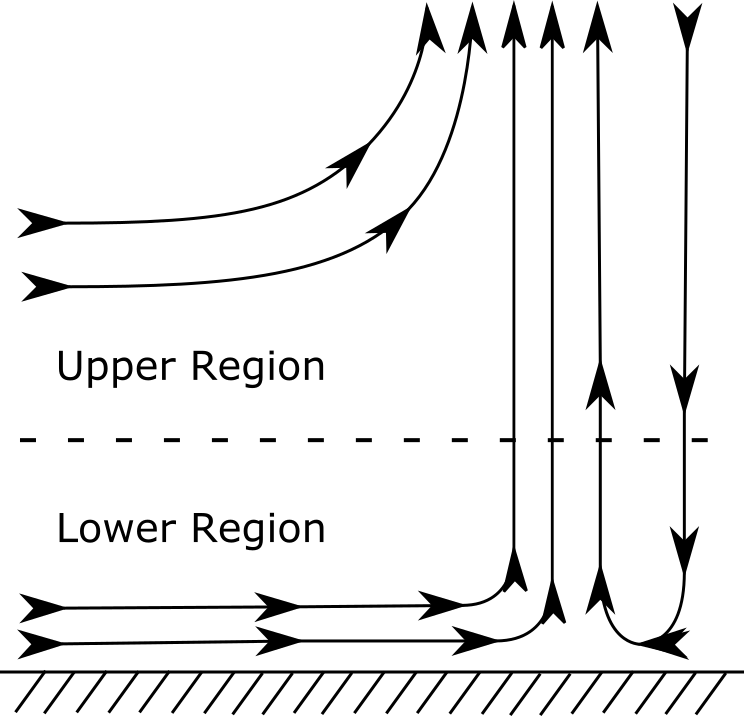
\includegraphics[width = 10 cm]{figs/ground}
     \caption{Cartoon of the structure of a dust devil. The lower region
     is the principle location of radial inflow, with the higher second
     layer flow becoming entrained by the upwardly circulating
     vortex. Notice also the downward flow in the center of the vortex.}
     \label{fig:cartoon}
    \end{center}
  \end{figure}


Renewed interest in naturally occurring dust devils has resulted from
the observation of them on Mars, first photographed by the NASA's Mars
Reconnaissance Orbiter\cite{}, and more recently by the Mars rover,
Opportunity. Their presence on Mars, with 1/100 of the atmospheric
density of the Earth, speaks to the universal character of the
phenomenon. Due to the greatly decreased atmospheric density, the
Martian dust devils are substantially larger, ranging several kilometers
across at their base and over ten km tall. 

interest in mixing and

There is lots of activity on dust devils and dust electrification now.  
The reason for this is that the ExoMars Lander will measure electric fields on Mars.

Numerical simulations of dust devils have been previously
reported.\todo{expand this greatly} However, they are typically large
eddy simulations (LES) that point towards the spontaneous occurance of
similar phenomena within existing 
climate and atmospheric
models\cite{QJ:QJ200513160722,doi:10.3137/ao.420105}. 


It is not clear what generates the azimuthal velocities. Two major
hypotheses as to the behavior exist. The first is that that ambient
vorticity in the atmosphere is drawn into the vortex from the far field,
and intensifies due to vortex stretching.\cite{} 

The other is that vortex tilting\cite{}

\section{Estimate of Energy Scaling}

Here we provide a rough estimate of the energy
available to a dust devil. There are two objectives of this
analysis. The first is to provide justification for the concept of
extracting energy from them, with the reasoning that should
sufficient energy be available, then attempting to extract it might be
worthwhile. The second objective is to provide a simple analysis that
can serve as a measure of the efficiency of the generation process,
e.g. ``What fraction of the available energy are we extracting?''.  

Steady state conditions requires that the dust devil not
extract more energy than is provided by the thermal resource, the Sun.   
The peak direct solar insolation in Arizona on a hot summer day is
greater than 1000 $W/m^2$. However, this estimate is problematic. 
It is in some sense an optimistic upper bound, as dust devils are only
converting a fraction of this solar resource into kinetic
energy. Renno and Ingersoll\cite{renno_inger} used an idealized heat
engine frame-work to study natural convection and to propose a theory
for convective available potential energy (CAPE), however, the
predictions from this underestimate the observed velocities in the real
objects. Furthermore, It is not clear how large of a region that dust
devils draw their energy from. Finally, dust devils are highly
intermittent creatures, typically existing only for a short time. It is
not certain that they are able to be accurately represented in a steady
state context. Lending some credence to this are the measurements of
\cite{} which found that surface heat fluxes could rise to . 

Sinclair's measurements of the velocity profiles inside a dust 
devil provides a more direct estimate. A velocity profile taken 
at approximately 9 meter height is shown in Figure \ref{fig:sinclair_profile}. 

  \begin{figure}[!htb]
    \begin{center}
     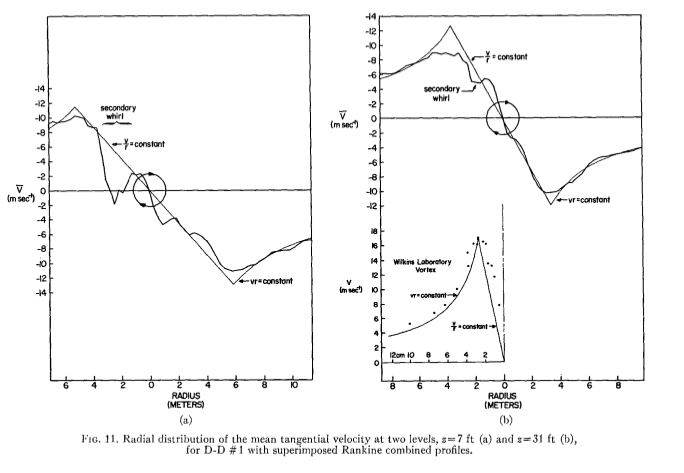
\includegraphics[width = 20 cm]{figs/sinclair_cut}
     \caption{Sinclair Profile}
     \label{fig:sinclair_profile}
    \end{center}
  \end{figure}

This is a dust devil with an inner core radius of approximately 
6 meters, and tangential and axial velocities of 11 and 10 m/s, respecively. 
This profile can be integrated to provide an estimate of the power though this plane, 
\begin{equation}
 P = -\frac{\rho }{2} \int V_z (V_{\theta}^2 + V_z^2 ) dA, 
\end{equation}
which results in an estimate of 24 kW. This is a substantial amount of
energy. 

%
% show what sinclair measured, then show how we think these energies
% break down into kinetic vs wind
%

As alluded to above, the energy composition of these flows is of
interest. For instance, Carroll and Ryan\cite{JGR:JGR14185} %1970
found that the kinetic energy contained within a dust devil exceeds that
which is attributable to buoyancy. Furthermore, Kaimal and Busigner
observed that dust devils possessed an order of magnitude greater
vertical flux in kinetic and than similarly sized convective
plumes~\cite{doi:10.1175/1520-0450(1970)009<0612:CSOACP>2.0.CO;2}. The
interplay between rotation, ambient winds and thermal potential energy
are critical to velocity intensities observed in these phenomena. 

As an example of this, consider only the energy flowing into the
entrainment region due to the ambient conditions, in particular, the
incoming wind and heat flowing through a cylindrical region. A
medium-sized (3m radius) dust devil with an incoming 
freestream velocity of 5 m/s. The surface temperature is 343 Kelvin,
with a specified inflow boundary layer bridging the ground temperature
to the ambient air conditions of 313 Kelvin.\todo{convert to same as
estimate above?}
% cite this?
\footnote{\normalsize These numbers were selected based on information
provided by the Georgia Tech field team from measurements performed in
Arizona during the summer of 2014.} 

There are two forms of energy to consider: kinetic and gravitational
potential. First, we examine the kinetic energy flux through the front
of the apparatus. 
%From the first law of thermodynamics we can express
The kinetic energy flux is a surface integral over the upstream face of
the device,  
\begin{equation*}
\text{KE} = \int \frac{\vec V^2}{2} \rho \vec V \cdot \hat n \, dA.
\end{equation*}
%
% could cite fluid dynamics book here
% pg. 239
%
Several simplifying assumptions are made. The freestream 
velocity is assumed to have no components in the span and height and
the variation in height of the streamwise
velocity is only due to the thin boundary layer near the
ground. The boundary layer profile is modeled using the common 7th
power function for a turbulent boundary layer,  
\begin{equation*}
  u(z) = U \text{ min }\left(\left(\frac{z}{\delta}\right)^7,1\right)
\end{equation*}
where U is the constant freestream velocity and $\delta$ the assumed
boundary layer thickness. 
The result for the kinetic energy is then, 
\begin{align*}
\text{KE} & = R \rho U^3 \left[ z_{\text{max}} - \frac{10}{11}\delta
\right].
\end{align*}
Where R is the radius of the vortex. Typical values of these quantities
are, $U = 5$ m/s, $\rho = 1.225$ Kg/$\text{m}^3$, $R = 3$ m,
$z_{\text{max}} = 2.5$ m and $\delta \approx 10$ cm. This provides an
estimate of 1144 Watts as the incoming kinetic energy flux. 

The gravitational potential energy flux is estimated by integrating the
boussinesq potential energy flux over the upstream flow. 
This is the maximum energy that could be extracted from the flow by an 
adiabatic redistribution of the density variation from the ambient 
density of the freestream flow, $\rho_\infty$. 
This potential energy ($E_p$) has the form of a surface integral over 
the front half of the vanes, 
\begin{align*}
  E_p & = \int u(z) (\rho(z)-\rho_\infty) g z dA. 
\end{align*}
As the density only varies with height, the integral is simplified to only vary in 
this direction
\begin{align*}
  E_p  & = g \int^{z_\text{max}}_0 u(z) (\rho(z)-\rho_\infty) \, z  \pi
 R \, dz.
\end{align*}
Using the bousinesq approximation, $(\rho(z)-\rho_\infty)  = \rho_0 \beta \Delta T$,
%\begin{align*}
%   (\rho(z)-\rho_\infty) & = - \rho_0 \beta \Delta T 
%   (\rho(z)-\rho_\infty) & = - \rho_0 \beta (T(z) - T_\infty),
%\end{align*}
the integral becomes, 
\begin{align*}
  E_p & = g  \pi R \beta \rho_0 \Delta T \int^{z_\text{max}}_0 u(z) \, z dz.
\end{align*}
This is solved to show
\begin{align*}
  E_p & = g  \pi R \beta \rho_0 U \Delta T \left[ \frac{z_\text{max}^2}{2} - \frac{7 \delta^2}{18} \right].
\end{align*}

%
% \todo{check units}
% 
% lets check the units here--
%
% m/s m^3 1/T kg/m^3 m/s T
%
% = Kg M^2 / s^3
%

%Once again assuming the 7th order power function for a turbulent boundary layer, 
% old text:::
%% \begin{align*}
%%   \text{Potential Energy Flux} & = \int_{-z_\text{max}}^0 u(z) \Delta \rho g z dz. \\
%%   & = \int_{-z_\text{max}}^0 u(z) \rho' g z^2 dz. 
%% \end{align*}
%% Where the substitution, $\Delta \rho = \rho' z$ was made. We again
%% assume the boundary layer follows the 7th order profile, and 
%% that $\rho' = -\beta \rho_0 \Delta T$, resulting in, 
%% %
%% % cite monin-yaglom page 59
%% %
%% \begin{equation}
%%  \text{Power } = U \beta \rho_0 \Delta T g \left[ \frac{z_\text{max}^3}{3} -
%% 					    \frac{7}{30} \delta^3
%% 					   \right]. 
%% \end{equation}

Characteristic values for a dust devil are $\rho_0 = 1.225$ Kg/$\text{m}^3$, 
$\Delta T= 30$ Kelvin, $\beta = 0.003194$ (This is 1/$T_{\text{ground}}$), 
$R = 3 $ m, $z_\text{max} = 2.5$ m, $\delta \approx 10$ cm, $g=9.81$ m/$s^2$, and a
freestream velocity of five meters per second results in an estimate of 34 Watts %33.82 Watts 
for the gravitational potential energy. 

The majority of the available energy is thus in the kinetic energy of
the wind, not the gravitational potential energy of the actual air. 
% todo: think about renno
%This is inconsistent with the results of
%Renno\cite{}\todo{missing cite here}, who demonstrated
%that the available thermal energy present was not sufficient to account
%for the velocities measured in dust devils. 
However, while the gravitational potential energy is a small fraction of
the energy available, that does not imply it is without significant
impact. 
%The extent to which the thermal energy acts as an assisting mechanism for 
%``lifting-up'' the flow is unclear, but 
Given the observed increase in dust devil formation during peak thermal
gradients, it is expected to play an important role. 

\section{Previous Concepts for Extracting Gravitational Potential
 Energy}

cite\todo{des it even make sense to write much here?}

cite\todo{cite mark thesis}

%
% https://en.wikipedia.org/wiki/Vortex_engine
%
% https://en.wikipedia.org/wiki/Solar_updraft_tower
%
% https://upload.wikimedia.org/wikipedia/commons/8/8b/Smoke-jack.jpg
%
% http://vortexengine.ca/AVE_FAQ.shtml
%
% http://ir.lib.uwo.ca/etd/89/
%
% http://www.popsci.com/technology/article/2012-12/paypal-cofounder-funds-tornado-harnessing-power-generator-produce-cheap-clean-energy
%
% Philosophies and fallacies in turbulence modeling --citation
%
% http://www.numerik.uni-hd.de/Oberwolfach-Seminar/CFD-Course.pdf
%

\section{Dust Devil Generation Concept}

The preceding discussion suggests that dust devils are carriers of
significant levels of ambient kinetic and gravitational potential energy
from the environment. This subsection provides a brief discussion of how
the physics of dust devils informs the generation of a synthetic
variety, that might be used as a means of extracting usable work.  

In contrast to the naturally occuring dust devils,
our synthetic solar driven vortex (SoV) design makes use of
control surfaces. These turning vanes also serve as an anchor for the
synthetic vortex, locking it into a small region. An abstract concept of
the turning vane geometry is shown in Figure \ref{fig:cartoon_vanes}.

  \begin{figure}[!htb]
    \begin{center}
     \includegraphics[width = 8 cm]{figs/ground_vanes}
     \caption{Image of a possible two tier turning vane 
       configuration for generating synthetic dust devils. This image depicts a 
       vertical slice through the proposed configuration, and does not show the reflection 
       of the two tier turning vanes, which would be expected to encircle the dust devil core.}
     \label{fig:cartoon_vanes}
    \end{center}
  \end{figure}

% Our observations of the naturally occuring dust devils informs some of
% our \textit{a priori} expectations for the design of the turning
% vanes. The bottom tier are designed to reside in the lower region, where
% the principle inflow will occur. We therefore expect a radial or nearly
% radial start to the vanes, which becomes increasingly tangential as the
% flow moves towards the center. The inner radius of the bottom tier will
% correspond to the outer radius of the generated vortex. 

% The top tier serves a different purpose. We expect a non-zero initial
% angle, as this tier is also designed to protect the rising vortex from
% being blow away by ambient winds. The vanes radius will be shorter, as
% the flow from this tier becomes entrained and the vortex grows in
% size. 

% For both the upper and lower tiers, our objective is to strike a balance
% between effectively turning the incoming flow to impart azimuthal
% velocity, while simultaneously not introducing such a high angle that
% the vanes act as a blocking surface which the incoming flow will move
% around. For instance, when the inlet angles are too severe, the vanes
% block the incoming flow, which results in an adverse pressure gradient
% existing near the outside edge of the 
% vanes. This serves to force fluid around and over the system, instead
% of inside the turning vanes. This reduces the velocity of flow inside
% the system, resulting in a weaker thermal vortex.  To reduce
% the flow blockage, we use gently curving vanes. A gentler angle permits
% more flow to enter the vane region, after which the curvature increases
% toward the center of the vanes. In this way, the angle smoothly varies
% between a nearly zero angle at the outside edge of the vanes to a
% maximum angle at a specified inner radius.

The characteristics of natural dust devils shown in Figure
\ref{fig:cartoon} suggest that the turning vanes be structured with two
tiers (see Figure \ref{fig:cartoon_vanes}). The lower tier would be
designed to manipulate the surface layer 
that lifts up into the core of the vortex, while the upper tier would
control entrainment into the vortex. In both tiers, the design of the
turning vanes must balance between the need to turn the flow from the
radial direction to the azimuthal direction to create vortical motion
and the requirement to not block flow into the vortex. Furthermore, in
the presence of a cross wind, the vanes need to prevent flow that
would pass right through the device, which would disrupt the vortex.
Finally, in field tests of design concepts for a solar vortex device
conducted by our colleagues at the Georgia Tech, it was found that cross
winds over the facility will also disrupt the vortical flow, and that
this could be controlled by introducing a conical wind-block on top of
the upper tier of vanes. One such field test configuration is shown in
Figure \ref{fig:field_test}. Within this broad conceptual design, there
remains a large design space to explore, including design parameters for
both tiers of vanes and the wind-block cone.

  \begin{figure}[!htb]
    \begin{center}
     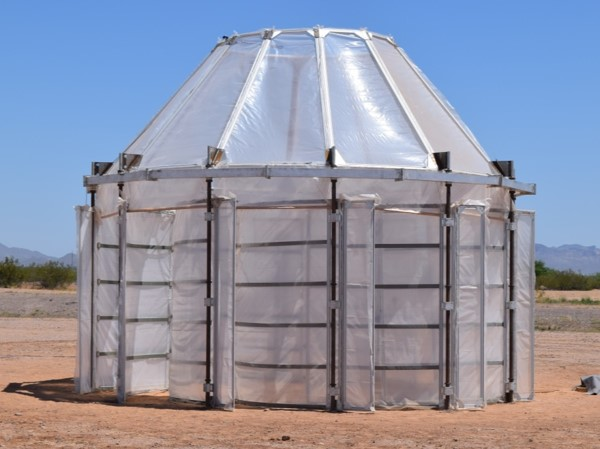
\includegraphics[width = 8 cm]{figs/sov_field}
     \caption{An image of the field configuration from the June, 2015
     tests in Arizona. The second (upper) tier of vanes and the cone are
     clearly visible. This apparatus has an outer diameter of
     approximately three meters.}
     \label{fig:field_test}
    \end{center}
  \end{figure}

To extract energy from the synthetic dust devil formed by the vane
system described briefly above, a turbine would be placed near the top
of the upper vanes. The turbine would extract energy from both the
vertical and azimuthal flow in the vortex, and so the design
considerations are different from those for a classical wind turbine.
Furthermore, there is presumably an analog to the Betz limit on how
much of the energy can be extracted, without disrupting the flow so
much that the vortex cannot be maintained. This will need to be
explored as part of the turbine design process.

In the research proposed here, the design and performance of a dust
devil energy harvesting system will be explored using computational
models. Computer models will enable a more extensive exploration of
the design space than would be possible experimentally. The design
concept described above will be analyzed to maximize the the
power that can be generated by the system and to develop scaling
describing how power depends on device size, wind speed and thermal
conditions. Further new design concepts that may be formulated will
also be evaluated. The subsequent section will provide the mathematical
representation used to model the system.  

%
%
%

% Our principle objective is to use a synthetic dust devil to produce 
% usable work. To extract the energy from the synthetic dust
% devil, a turbine is placed 
% at or near the top of the second tier of turning vanes. 
% The blades of the turbine will be driven by the dust devil's azimuthal
% and vertical velocities. While the Betz limit\cite{betz} gives a reasonable
% expectation of the efficiency with which energy can be expected to be
% extracted from the ambient dust devil velocity field, there are other
% non-trivial design considerations. In particular, the impact of the
% turbine on the dust devil's vortex, and any potential disruption of the
% flow on account of the turbine must be investigated. Optimizing the
% turbine to maximize the energy extraction while simultaneously
% minimizing it's impact on the character of the dust devil's solution
% will be an important issue.

% While the turning vanes and turbine  
% paradigm represents a reasonable starting point for design, the
% parameter space of possible system configurations is large. It is
% unclear how to engineer an effective SoV system. Important design
% consideration include: 
% \begin{itemize}
%   \item How should the turning vanes be configured?
%   \item How does the energy produced scale with system diameter?
%   \item Are additional surfaces, such as a cone, capable of increasing energy output?
% \end{itemize}

% Questions such as these provide the principle impetus of using
% computational fluid dynamics (CFD) to inform system design. The
% parameter space of conceivable system designs is far larger than can be
% probed experimentally, and even if such a campaign were to be embarked
% upon, it would be at significantly greater temporal and monetary
% cost. The subsequent chapter will provide the mathematical basis by which
% we model the system, so that we can then begin to discuss how we might
% optimize it computationally.  




\chapter{Mathematical Models}
%\section{Mathematical Modeling}
\label{sec:mathmodel}

% \begin{itemize}
% \item \st{unstable stratified boundary layers (raleigh number estimate)}
% \item \st{justify incompressible N-S}
% \item \st{justification of far-field eddy-viscosity model (M-O)}
% \item modeling eddy-viscosity in device 
% \item vane and turbine representation via penalty function // immersed boundary method
% \item cone representation
% \end{itemize}

%remember that \st{} is strikethrough
%
% should this all be math modeling?
%

The aim of this work is to simulate synthetic
dust devils in the field. This requires a model of the ambient
conditions for a representative case, such as Arizona, where
experimental data is available from tests that have been
performed. Furthermore, for this to be generally useful in the
prediction of flows in a variety of conditions, we need a model
applicable to any flow near the surface of the earth.  

This chapter details an analysis of surface fluid mechanics, and
develops a mathematical model for turbulence in a thermally stratified
medium. We seek to emulate the operation of the apparatus during the
day, when dust devils are observed to form readily. 
At these times, the atmospheric surface layer has the following
character. Incident radiation from the Sun does not significantly
interact with the air, which is nearly
transparent\cite{haltiner1957dynamical}. Instead, this radiation is
absorbed by the ground, which causes its temperature to rise. This
results in a temperature difference between the hot ground and the cooler
air. The sensible heat causes expansion and lowers the density
of the air. This reduced density air near the surface is then driven
upwards by buoyancy.    

For sufficiently large temperature differences, the hot surface layer is
unstable, and as the warm air is driven upwards the flow will transition
to turbulence. For the typical use case we consider, namely Arizona in
summer, the temperature difference can be in excess of 30 Kelvin. 
Rayleigh numbers associated with temperature differences of this
magnitude are between $10^{9} - 10^{11}$ and therefore meets the
criterion\cite{incropera1996fundamentals}  
for transition to a turbulent regime. The flow is that of an unstably
stratified fluid.  

This chapter begins by describing the governing equations of the system
of interest. It then proceeds to the development of a viscosity model
used to resolve the large scale features of the solution. Next, models
used to represent the vanes and turbine, are introduced.  Finally, the
models for the computational domain extent and the boundary conditions
are discussed. 

%Note that a complete numerical specification of all the model
%parameters introduced in this chapter are provided in a table in
%appendix \ref{app:model_param}.

\section{The Governing Equations of Fluid Motion}
\label{sub_sec:ns_en}

The equations describing fluid flow with natural convection are,
\begin{align}
  \frac{\partial {\bf u}}{\partial t} + {\bf u} \cdot \nabla {\bf u} =& \,
  -\frac{1}{\rho}\nabla P + \nu \nabla^2 {\bf u} - {\bf g} \frac{T'}{T_0}
 \label{eq:ns} \\
  \nabla \cdot {\bf u} =& \, 0 \label{eq:cont} \\
  \rho c_p \frac{\partial T}{\partial t} + {\bf u} \cdot \nabla T =& \, \nabla
 \cdot ( k \nabla T) \label{eq:ht}
\end{align} 
under the assumption that the temperature variation is small in
comparison to the mean temperature of the region. These are the
incompressible Navier-Stokes equations with the Boussinesq
approximation\cite{boussinesq2010théorie}, a representation of buoyancy
coupled with the heat equation. Note that in
Equations~\ref{eq:ns}-\ref{eq:ht}, and throughout this document,
boldface denotes a vector quantity, for example, ${\bf u} = \{u,v,w\}$.  
Further these equations ignore the action of the Coriolis force. 
Monin and Obukhov~\cite{monin1954basic} demonstrated that the Coriolis
force is negligible for the surface layer below fifty meters (a distance
well below our region of interest), and this argument is detailed in
Appendix~\ref{appendix:coriolis}.  

As discussed above, we anticipate that the flow will be sufficiently
high Reynolds number as to be
turbulent~\cite{Reynolds01011883}. Turbulence significantly alters the
character of the flow,  
and necessitates either resolving the resulting small scales or
providing a model that represents their impact. In this case, a
Reynolds Averaged Navier-Stokes (RANS) formulation is used, where the 
turbulent viscosity and thermal conductivities are permitted to vary in
space, and the flow is decomposed into constant laminar and varying
turbulent and vane components,\todo{not always rans}  

\begin{eqnarray*}
 \nu =& \nu_{l} + \nu_{T}(z) + \nu_{V}(r,z) \\
 K =& K_{l} + K_{T}(z) + K_{V}(r,z).
\end{eqnarray*}

This is an effective eddy viscosity model\cite{boussinesq1887}, and the
subsequent two sections will elaborate on the spatial dependence and
character of $\nu_T$, $K_T$, $\nu_C$ and $K_C$. The laminar, base
diffusivities are $\nu_l$ and $K_l$, which do not vary in space.  

\section{Viscosity Model}

We use the well-known similarity model of Monin and
Obukhov\cite{monin2007statistical,1990JFM...212..637K} as
a guide to the specification of an eddy viscosity model to describe the
vertical mixing in the atmosphere. This formulation is an extension of
the mixing-length model of Prandtl, where the concepts of gradient
diffusion and mixing length were generalized to thermally stratified
flow.    

%ADD DIMENSIONS TO MAKE SCALING MORE CLEAR\todo{add dimensions}
%
% justify prandtl assumption here
%

Monin and Obukhov argued that under statistically stationary, horizontally
homogeneous conditions, the dynamics of any mean turbulent quantity
($\bar f$) in a thermally stratified medium depend only on,  

\begin{equation}
\bar f = f(z,\frac{g}{T_0},\rho_0,\nu_l,K_l,u^*,q).
\end{equation}
Aside from near the surface, the laminar diffusivities $\nu_l$ 
and $K_l$ will be  
small compared to their turbulent counterparts, $\nu_T$ and $K_T$, and 
are therefore negligible. 
The remaining five parameters are: the distance from the ground, z; the
buoyancy coefficient, $\frac{g}{T_0}$; the density of the fluid,
$\rho_0$; a velocity scale, $u^*$ (in particular, the freestream
velocity); and the heat flux to the ground, $q$. %\todo{is this right?}
% Likewise, if we define $z-z_0$ as an ``effective roughness
% height'' or displacement distance, we can reasonably neglect $z_0$ from these
% considerations. While the roughness height can be large (for instance in
% a cornfield, where the roughness height could reasonably be several
% meters), for the present study the expectation is that this roughness
% height will be on the order of centimeters\cite{oke1987boundary}, and
% therefore negligible.  
%
% add refence to dynamical and physical meteorology 
% 
These primary quantities have the following dimensions,

\begin{eqnarray}
 \textbf{Height:}& z\enskip \dot = \enskip [m]  \\
 \textbf{Buoyancy:}& \qquad \frac{g}{T_0}\enskip \dot = \enskip [kg] [m] [s]^{-2}
  [K]^{-1} \\ 
 \textbf{Density:}&  \enskip \rho \enskip \dot = \enskip [kg] [m]^{-3}  \\
 \textbf{Velocity:}& \enskip u^* \enskip \dot = \enskip [m] [s]^{-1} \\
 \textbf{Heat Flux:}& \enskip q \enskip \dot = \enskip [kg] [s]^{-3} 
 %\textbf{Height:}& z \rightarrow \text{Units}: Meters \rightarrow [m]  \\
 %\textbf{Buoyancy:}& \frac{g}{T_0} \rightarrow Units: Meters \rightarrow
 % [m]  \\ 
 %\textbf{Density:}& \rho \rightarrow Units:  \rightarrow
 % [m]  \\ 
 %b & b
\end{eqnarray}

Our unknown mean turbulent quantity ($\bar f$) depends on four
dimensions: length, time, temperature and mass. Dimensional analysis
implies that this should then only be a function of a single dimensionless
group\cite{munson2012fundamentals}. This is chosen to be,
\begin{equation}
 \xi = -\frac{\kappa \frac{g}{T_0} \frac{q}{c_p \rho_0} z}{ {u^*}^3}.
\end{equation}
where $\kappa$ is the (dimensionless) Von-Karman constant. 
The physical meaning of this quantity bears some discussion.  
The numerator, $\kappa \frac{g}{T_0} \frac{q}{c_p \rho_0} $, is
proportional to the buoyant production of kinetic energy.  The
denominator, $\frac{{u^*}^3}{z}$, is a shear production rate. 

The non-dimensional group $\xi$ is typically cast into the following 
form, 
\begin{equation}
 \xi = \frac{z}{L_{M-O}}
\end{equation}
where $L_{M-O}$ is the famous, ``Monin-Obukhov'' length,
\begin{equation}
 L_{M-O} = -\frac{{u^*}^3}{\kappa \frac{g}{T_0} \frac{q}{c_p \rho_0}}. 
  \label{eqn_mo_length}
\end{equation}

This length can be interpreted as the vertical location
where the production of buoyantly generated kinetic energy is
approximately equal to the energy generated by wind shear. When the
magnitude of $L_{M-O}$ is large, the flow is dominated by shear effects,
and the impact of buoyancy is small. Conversely, a small magnitude of
$L_{M-O}$ implies that buoyant effects largely dominate the kinetic
energy production. Notice also that the sign convention in Equation
\ref{eqn_mo_length} is such that for the systems we consider ($q > 0$, heat
flux from the surface to the air), $L_{M-O}$ will always be
negative. This is as expected, as the convection from the high
temperature surface to cooler air is unstable. 

%The mean quantity $\bar f$ has a
%functional representation to the effect,
In this case, appropriately normalized mean turbulent quantities should
be functions of only the non-dimensional group 
\begin{equation}
 \frac{\bar f}{f_{MO}} = \phi(\frac{z}{L_{M-O}})
\end{equation}
with $f_{MO}$ a normalizing constant with units of $\bar f$, and $\phi$
is a function only of $\xi$. Monin-Obuhkov similarity theory has been
shown to apply to a wide variety of
quantities\cite{wyngaard2010turbulence}, but we consider the velocity
and temperature fields here.  
Furthermore, we are interested in the case where
$\xi<0$, which corresponds to heat flux from the ground into the
air. For instance, the mean velocity field would have scaling,
$\frac{u^*}{\kappa}$ and the temperature fields would be scaled as $T^*
= \frac{1}{\kappa u^*} \frac{q}{c_p \rho_0}$. In this way, the mean
velocity and temperature fields would have the form,  
\begin{eqnarray}
\bar u(z) = \frac{u^*}{\kappa} \phi_u(\frac{z}{L_{M-O}}) \\
\bar T(z) = T^* \phi_T(\frac{z}{L_{M-O}}).
\end{eqnarray}
As a result, the mean vertical gradients of the velocity and temperature are
necessarily, 
\begin{eqnarray}
\frac{\partial \bar u(z)}{\partial z} = \frac{u^*}{\kappa L_{M-O}}
 \varphi_u(\frac{z}{L_{M-O}}) \label{eq:uz} \\ 
\frac{\partial \bar T(z)}{\partial z} = \frac{T^*}{L_{M-O}}
 \varphi_T(\frac{z}{L_{M-O}}) \label{eq:tz}.
\end{eqnarray}
Notice that $\phi$ and $\varphi$ are different (unknown) universal functions. Eddy
viscosity is defined as, $u'v' = \nu_T \frac{\partial
u}{\partial z}$\cite{durbin2001statistical}, in which case, using
equation \ref{eq:uz}, it must scale as
\begin{equation}
 \nu_T = \frac{{u^*}^2}{\frac{\partial \bar u}{\partial z}} = \frac{u^*
  \kappa L_{M-O}}{\varphi_u(\xi)}.
\end{equation}
While eddy thermal diffusivity (defined as, $q = c_p \rho_0 K_T
\frac{\partial T}{\partial z}$) is 
\begin{equation}
 K_T = \frac{q/c_p \rho_0}{\frac{\partial \bar T}{\partial z}} = \frac{u^*
  \kappa L_{M-O}}{\varphi_T(\xi)}.
\label{eqn:eddy_kt}
\end{equation}
Note the difference between $\varphi_u$ and
$\varphi_T$, which for turbulent Prandtl numbers near unity (e.g. $Pr_T
\approx 1$) the functions will be identical. The asymptotic behavior of
the $\varphi_T$ and $\varphi_u$ at large and small values of $\xi$
provides guidance to the more general character of the functions. 
Our interest lies in the case where $L_{M-O} \leq 0$, which corresponds
to heat flux from the ground into the air.  
%

\subsection*{Case One: $\xi \to 0$}
The first case, $\xi \to 0$, is equivalent to the scenario where
$\frac{z}{L_{M-O}} \to 0$, or $L_{M-O}>>z$. This occurs as the heat flux
at the wall approaches zero ($q \to 0$) , which is simply ``free
convection''. This would correspond to a purely wind driven flow with no
thermal gradient. In this limit, the solution is expected to regain the
thermally-independent result, the pre-eminent ``log-law''. Start by
considering Equation~\ref{eq:uz} rearranged into a slightly different form, 
\begin{equation}
 \frac{\partial \bar u(z)}{\partial z} = \frac{u^*}{\kappa L_{M-O}} \varphi_u(\frac{z}{L_{M-O}}).
\end{equation}
After substituting $L_{M-O}=\frac{z}{\xi}$, 
\begin{equation}
 \frac{\partial \bar u(z)}{\partial z} = \frac{u^*}{\kappa z} \xi \varphi_u(\xi).
\end{equation}
This is clearer if the substitution, $\Phi(\xi) = \xi \, \varphi(\xi)$, is made,
\begin{equation}
 \frac{\partial \bar u(z)}{\partial z} = \frac{u^*}{\kappa z} \Phi(\xi).
\end{equation}
One can now more easily see that this function results in a logarithmic
profile when $\Phi(\xi) = 1$, which in turn implies that for neutral
stratification $(\xi = 0)$, 
\begin{equation}
 \Phi(0) = \lim_{\xi \to 0} \, \xi \, \varphi(\xi)= 1. 
\end{equation}
We expect this to be approximately true for all small values of
$\xi$, e.g. 
\begin{equation}
 \Phi(\xi) \approx \text{ln } \rvert \frac{z}{L_{M-O}} \rvert + C 
\end{equation}
 when $ |\frac{z}{L_{M-O}}| << 1$. Identical arguments can be made for the
 asymptotic behaviour of the temperature function.

\subsection*{Case Two: $\xi \to -\infty$}

The case where $\xi \to -\infty $ implies $\frac{z}{L_{M-O}} \to
-\infty $ and $z>>L_{M-O}$. This is most readily interpreted as the instance
where $u^* \to 0$, e.g. the buoyancy-dominated case with no wind
(free-convection). This condition is typically referred to as,
``Thermal-only'' in this text. 
For this case, the function $\varphi_T$ must have no
dependence on $u^*$, and will approach a constant. Scaling
analysis implies that the overall function will not depend on $u^*$ only
when the function $\varphi$ scales to the $-\frac{4}{3}$ power. The
function must then be

\begin{equation}
 K_T = \frac{1}{C_T} \left( \frac{q}{c_p \rho_0} \frac{g}{T_0}
		     \right)^\frac{1}{3} z^{\frac{4}{3}}  \text{ 
for } z \gg L_{M-O}. 
\end{equation}

So long as the turbulent Prandtl number remains constant in space, a
realistic assumption~\cite{chuang1969turbulent}, then 
identical arguments regarding the asymptotic behaviour at large $\xi$
provide the analogous result for the eddy viscosity's variation with
respect to distance from the ground,   
\begin{equation}
 \nu_T = \frac{1}{C_{\nu_T}} \left( \frac{q}{c_p \rho_0} \frac{g}{T_0}
			     \right)^\frac{1}{3} z^{\frac{4}{3}}  \text{ 
for } z \gg L_{M-O}. 
\end{equation}


\subsection*{Approximations of the Universal Function}

We have now derived two criterion that our desired function of $\xi$ 
must capture. Namely, that for small values of negative $\xi$, the
function should be nearly identical to the logarithmic profiles
associated with neutral stratification. Secondly, at large negative
values of $\xi$, the function should approach a constant value. Finally,
we desire that the function smoothly vary between these conditions. 

Again following the lead from Monin-Obukhov, most functions are
formulated in terms of $\Phi(\xi)$, not $\varphi(\xi)$. Note that as
$\varphi(\xi) \thicksim \xi^{-\frac{4}{3}}$, and recalling that
$\Phi(\xi) = \xi \, \varphi(\xi)$, we expect 
$\Phi(\xi) \thicksim \xi^{-\frac{1}{3}}$.

There are several different functions, which are essentially different
calibrations of the same underlying function for different regimes with 
varying relative merits. %\cite{?}.\todo{missing cites} 
However, the functions are generally in close agreement under neutral
and unstable conditions, with the disagreement primarily occuring for
$z/L>0$. As we expect to only simulate conditions of unstable or
neutrally stratified flow, our choice of interpolation function does not
have a significant impact on the predicted value.  

\begin{figure}[!htb]
 \centering
  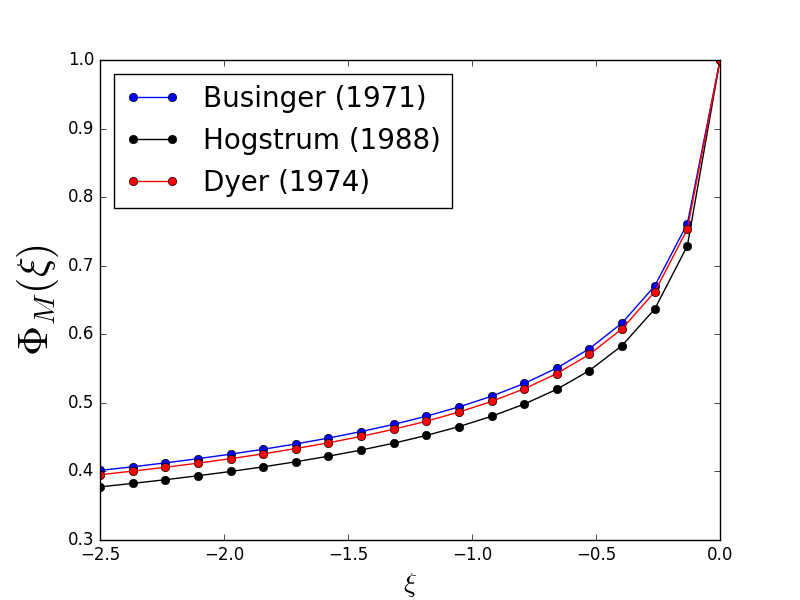
\includegraphics[width=.7\linewidth]{figs/mo-compare}\\
 \caption{Comparison between three common interpolation functions for
 the Monin-Obukhov universal function of momentum. The plots closely
 coincide, as the functions are generally in close agreement under
 neutral and unstable conditions, with the disagreement primarily
 occuring for $z/L>0$, which is unimportant for this work.} 
 \label{fig:interp-mo}
\end{figure}

Figure~\ref{fig:interp-mo} shows three common interpolation  
functions, the Businger~\cite{businger1971flux},
H{\"o}gstr{\"o}m~\cite{hogstrom1988non} and Dyer~\cite{dyer1974review}
functions. All have similar qualitative form,   
and yield nearly identical predictions. As a result, we use functions
that are simple to compute. The original functions 
proposed by Monin and Obukhov were avoided, they had a discontinuity in
the derivative, and are more inaccurate than modern functions due due to
the fact that they were calibrated on less accurate experimental
data. The H{\"o}gstr{\"o}m functions for momentum and temperature are, 
\begin{eqnarray}
  \Phi_M(\xi) =& (1-19.3 \, \xi)^{-1/4}, \\
  \Phi_T(\xi) =& 0.95 \, (1-11.6 \,\xi)^{-1/2}.
\end{eqnarray}
These functions have been found to be broadly applicable, accurate and 
are easily instantiated in software. For this reason the
H{\"o}gstr{\"o}m functions are used in this work. 

\subsection{Shortcomings of Monin-Obukhov Theory}

There are several well-known conditions for which the Monin
Obukhov similarity theory breaks down. These include:
 
\begin{itemize}
 \item Surfaces with large spatial variations in roughness
 \item Outside of the surface layer (several hundred meters) where the 
       coriolis effect is no longer negligible
%\item the theory's predictions are well known to be sensitive to choice
%      of universal function for $L>0$.
\end{itemize}

But neither of these are relevant here. 
In ``ideal'' situations, the theory has been found to be
accurate to better than 10\%\cite{QJ:QJ49709741204,kaimal}. 
For our case, with minimal surface roughness and our interest
constrained to the near surface layer, these functions are applicable
and reasonably accurate\cite{Foken2006}, and are easily implemented in
software.  

\section{Eddy Viscosity in the Device}

%However, this is also a more
%difficult regime to model.\todo{poor justification} 
The validation process identified a refinement to the virtual vane
formulation that results in a better representation of the vane
effects in a broader range of flows. The model uses an
enhanced turbulent diffusivity in the vortical plume region to account
for the effects of vortex shedding from the trailing edge of the vanes,
which is not represented in the virtual vane representation (discussed in
\ref{subsec:vane}). 

% To successfully accomplish this, source terms
% for production of diffusivity were formulated to properly
% account for the generation of turbulence in the region of the
% vanes. This diffusivity would then convect and diffuse through space. 
% To avoid modeling a temporal and three-dimensionally spatially
% varying field of diffusivities, we have instead calibrated the field
% based on data provided by our partners at Georgia Tech. 

%This calibration
%is detailed in Section~\ref{sec:validation}. 
The eddy-viscosity in the region of the vanes and interior is set based
on scaling relations for a turbulent self-similar circular jet, as
described in Pope\cite{pope2000turbulent},
 
\begin{equation}
  \nu_C = U_0 y_{1/2} \bar \nu_C.
  %\nu_C(r) = U_0(r) y_{1/2}(r) \bar \nu_C
\end{equation}

In this equation, $U_0$ is the peak velocity, and $y_{1/2}$ the jet
half-width (taken to be the dust devil half-width).  
% In words, we are scaling the
% calibrated viscosity by the velocity and length scale of the
% apparatus. $\bar \nu_C $ is input, measured from the experimental
% laboratory.  The diffusivity here is essentially a top hat filter, which
% radial values interior to the vanes the nominal calibrated value, and
% those outside the vanes zero, e.g. $\nu_C(r>r_{\text{vane}})=0$. 
The dimensionless constant $\bar \nu_C $ is calibrated based on
experimental data, and is set to zero outside the device. 
The thermal diffusivity inside the device, $K_C$, is then fixed with the 
assumption that the Prandtl number is unity.  

%The thermal and momentum diffusivities are expected to be even larger in the
%device where the flow across the vanes produces shear and generates
%turbulence. Our model for the diffusivities inside the vanes should
%therefore be higher than the ambient regions outside the vanes. 


\section{Vane Representation}
\label{subsec:vane}
To rapidly prototype general system configurations, the
computations must be able to explore a large space of possible
geometries and settings. This presents a significant meshing and 
computational challenge if the detailed flow around the vanes is to be
computed. In the region near the vanes, where a no-slip boundary
condition is imposed, the flow will necessarily form a thin momentum
boundary layer. Resolving this boundary layer requires high resolutions
immediately adjacent to the walls. Changing the vane location requires
that a new mesh be generated. This is a significant
challenge, as the development of a new mesh often requires significant
human effort and time. Furthermore, the process is error-prone, 
and would require that each simulation using a new mesh undergo 
detailed solution verification. 


% Your text on the virtual vanes does not provide enough information to
% know exactly what we did. It is needlessly vague, and does not
% adequately connect to the real vane geometry. I propose the following
% more direct and more precise text. Further, the penalty nomenclature
% is inappropriate.

Instead, we have developed a modeling formulation that does not require
explicitly meshing the turning vanes, or any surface. These so-called
``virtual vanes'' are implemented as a body force that 
is applied in the annular region that contains the vanes. 

   \begin{figure}[!htb]
    \centering
    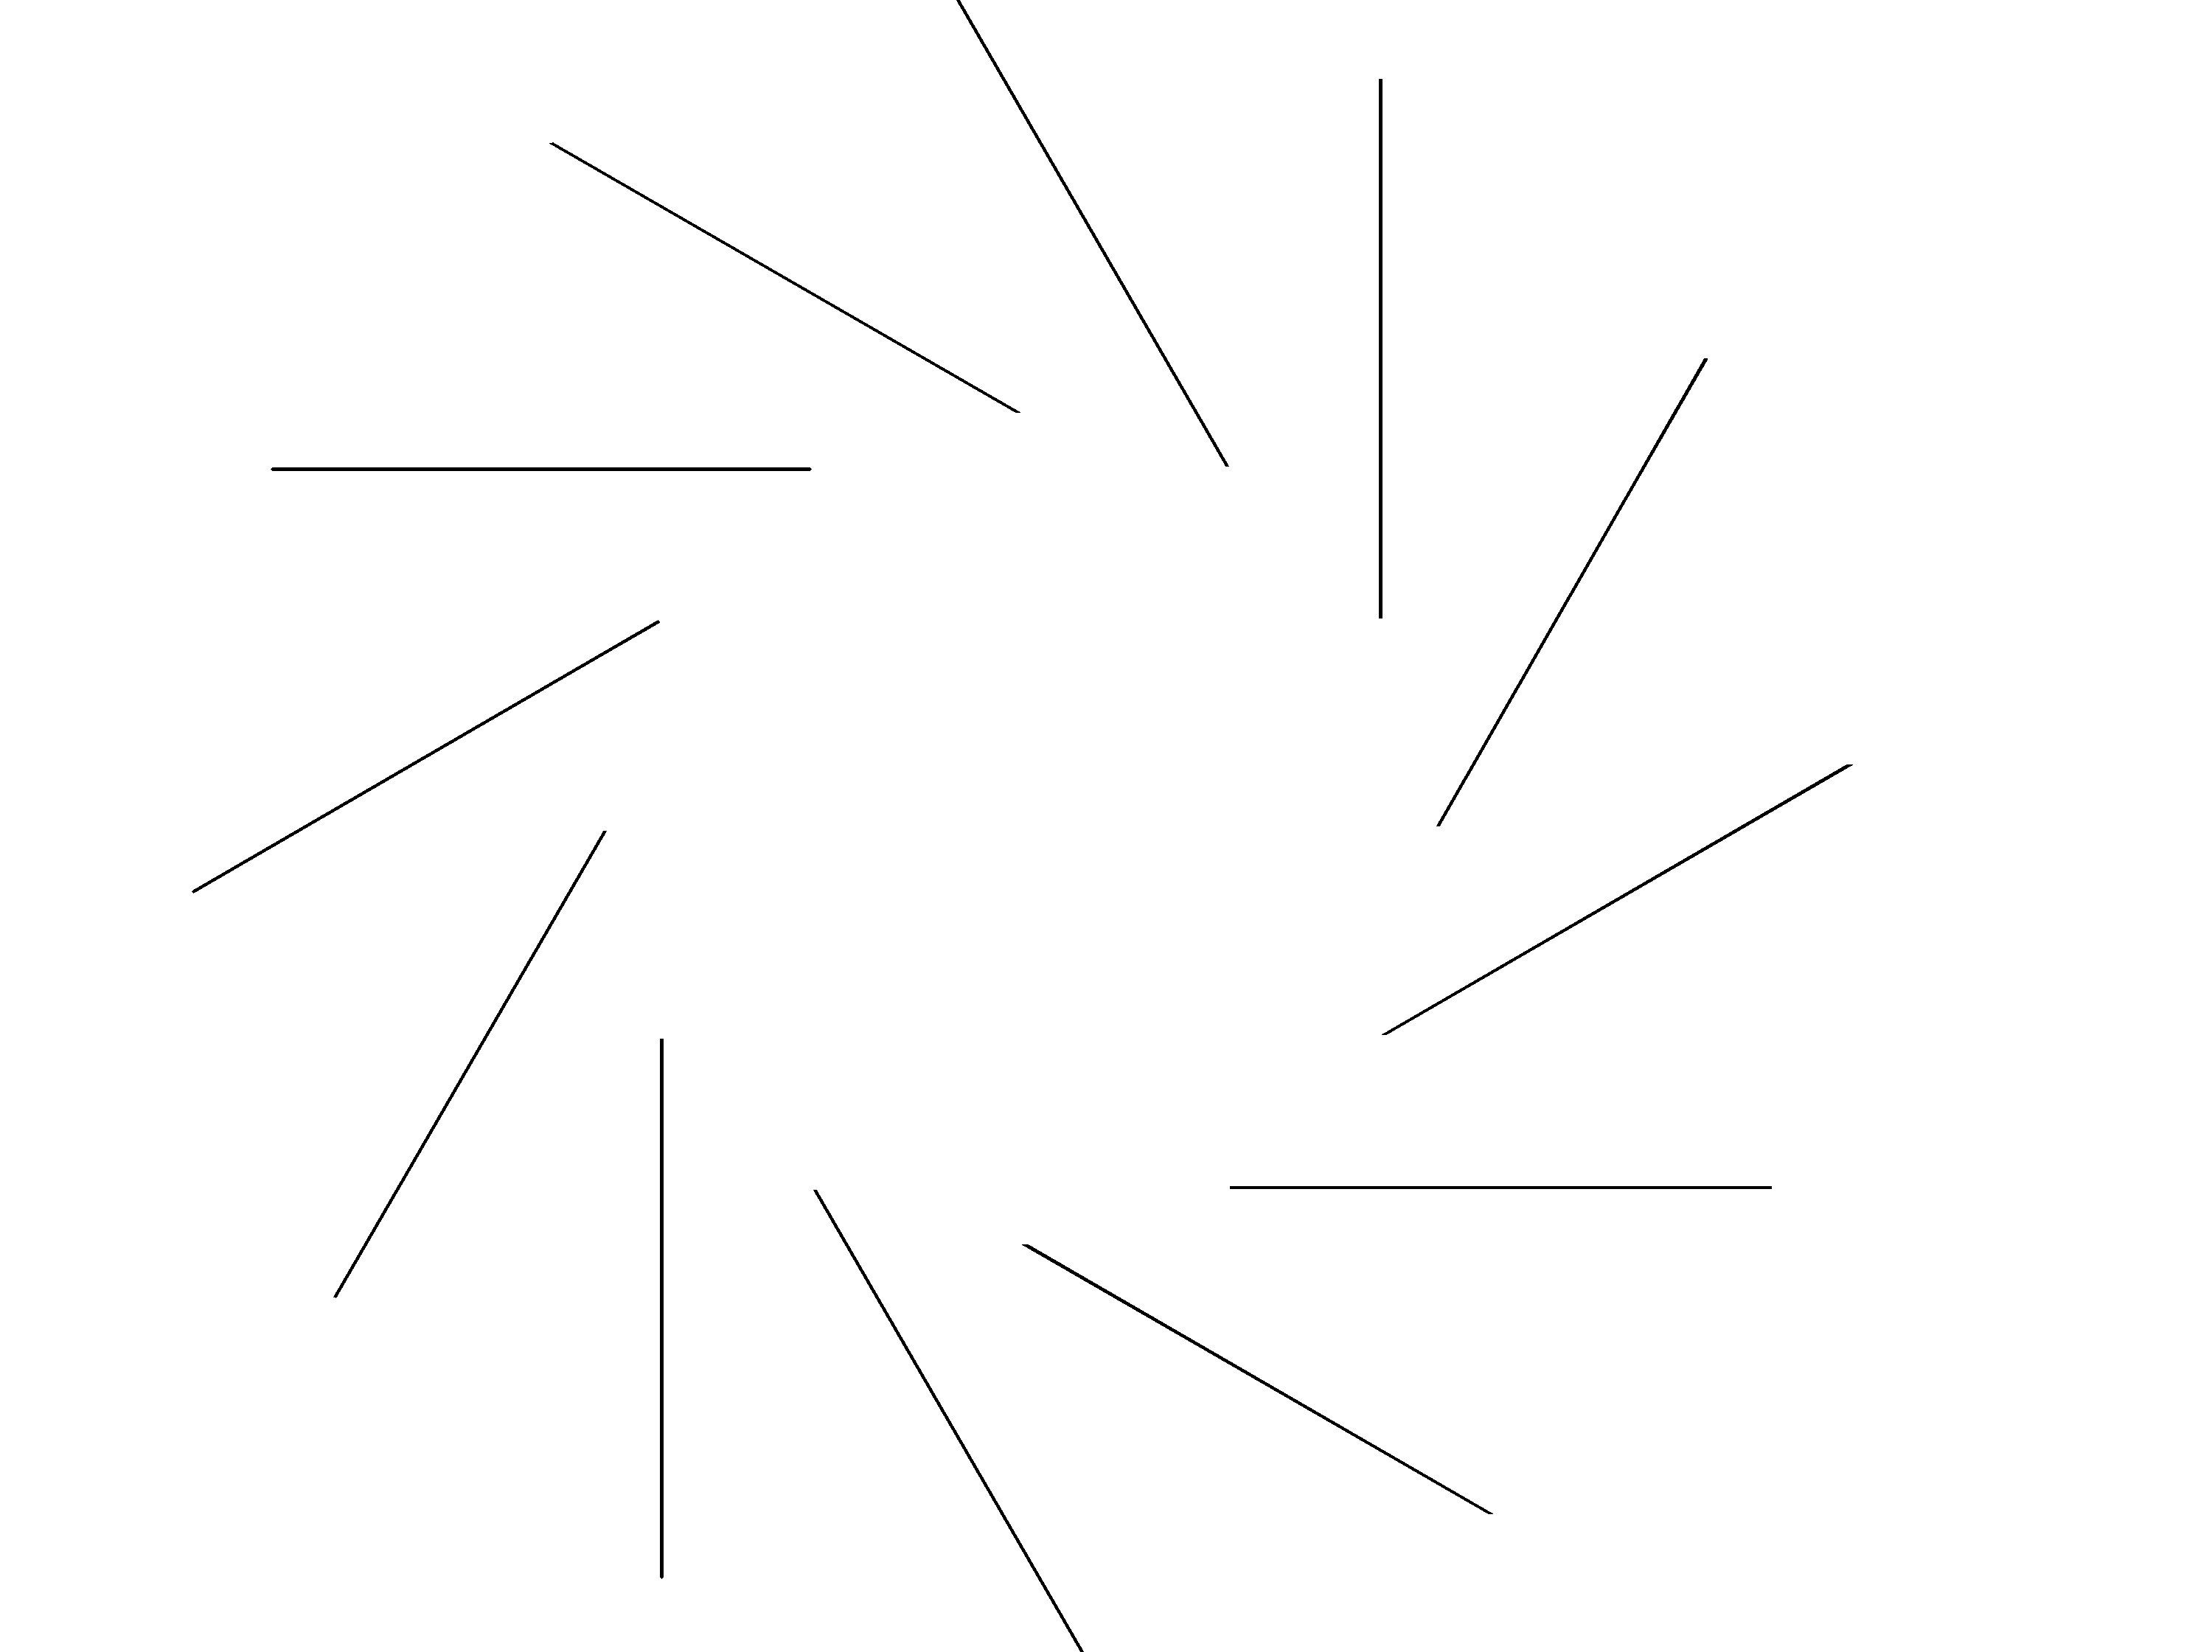
\includegraphics[width =0.47\textwidth]{figs/gridded_region}
    \hfill
    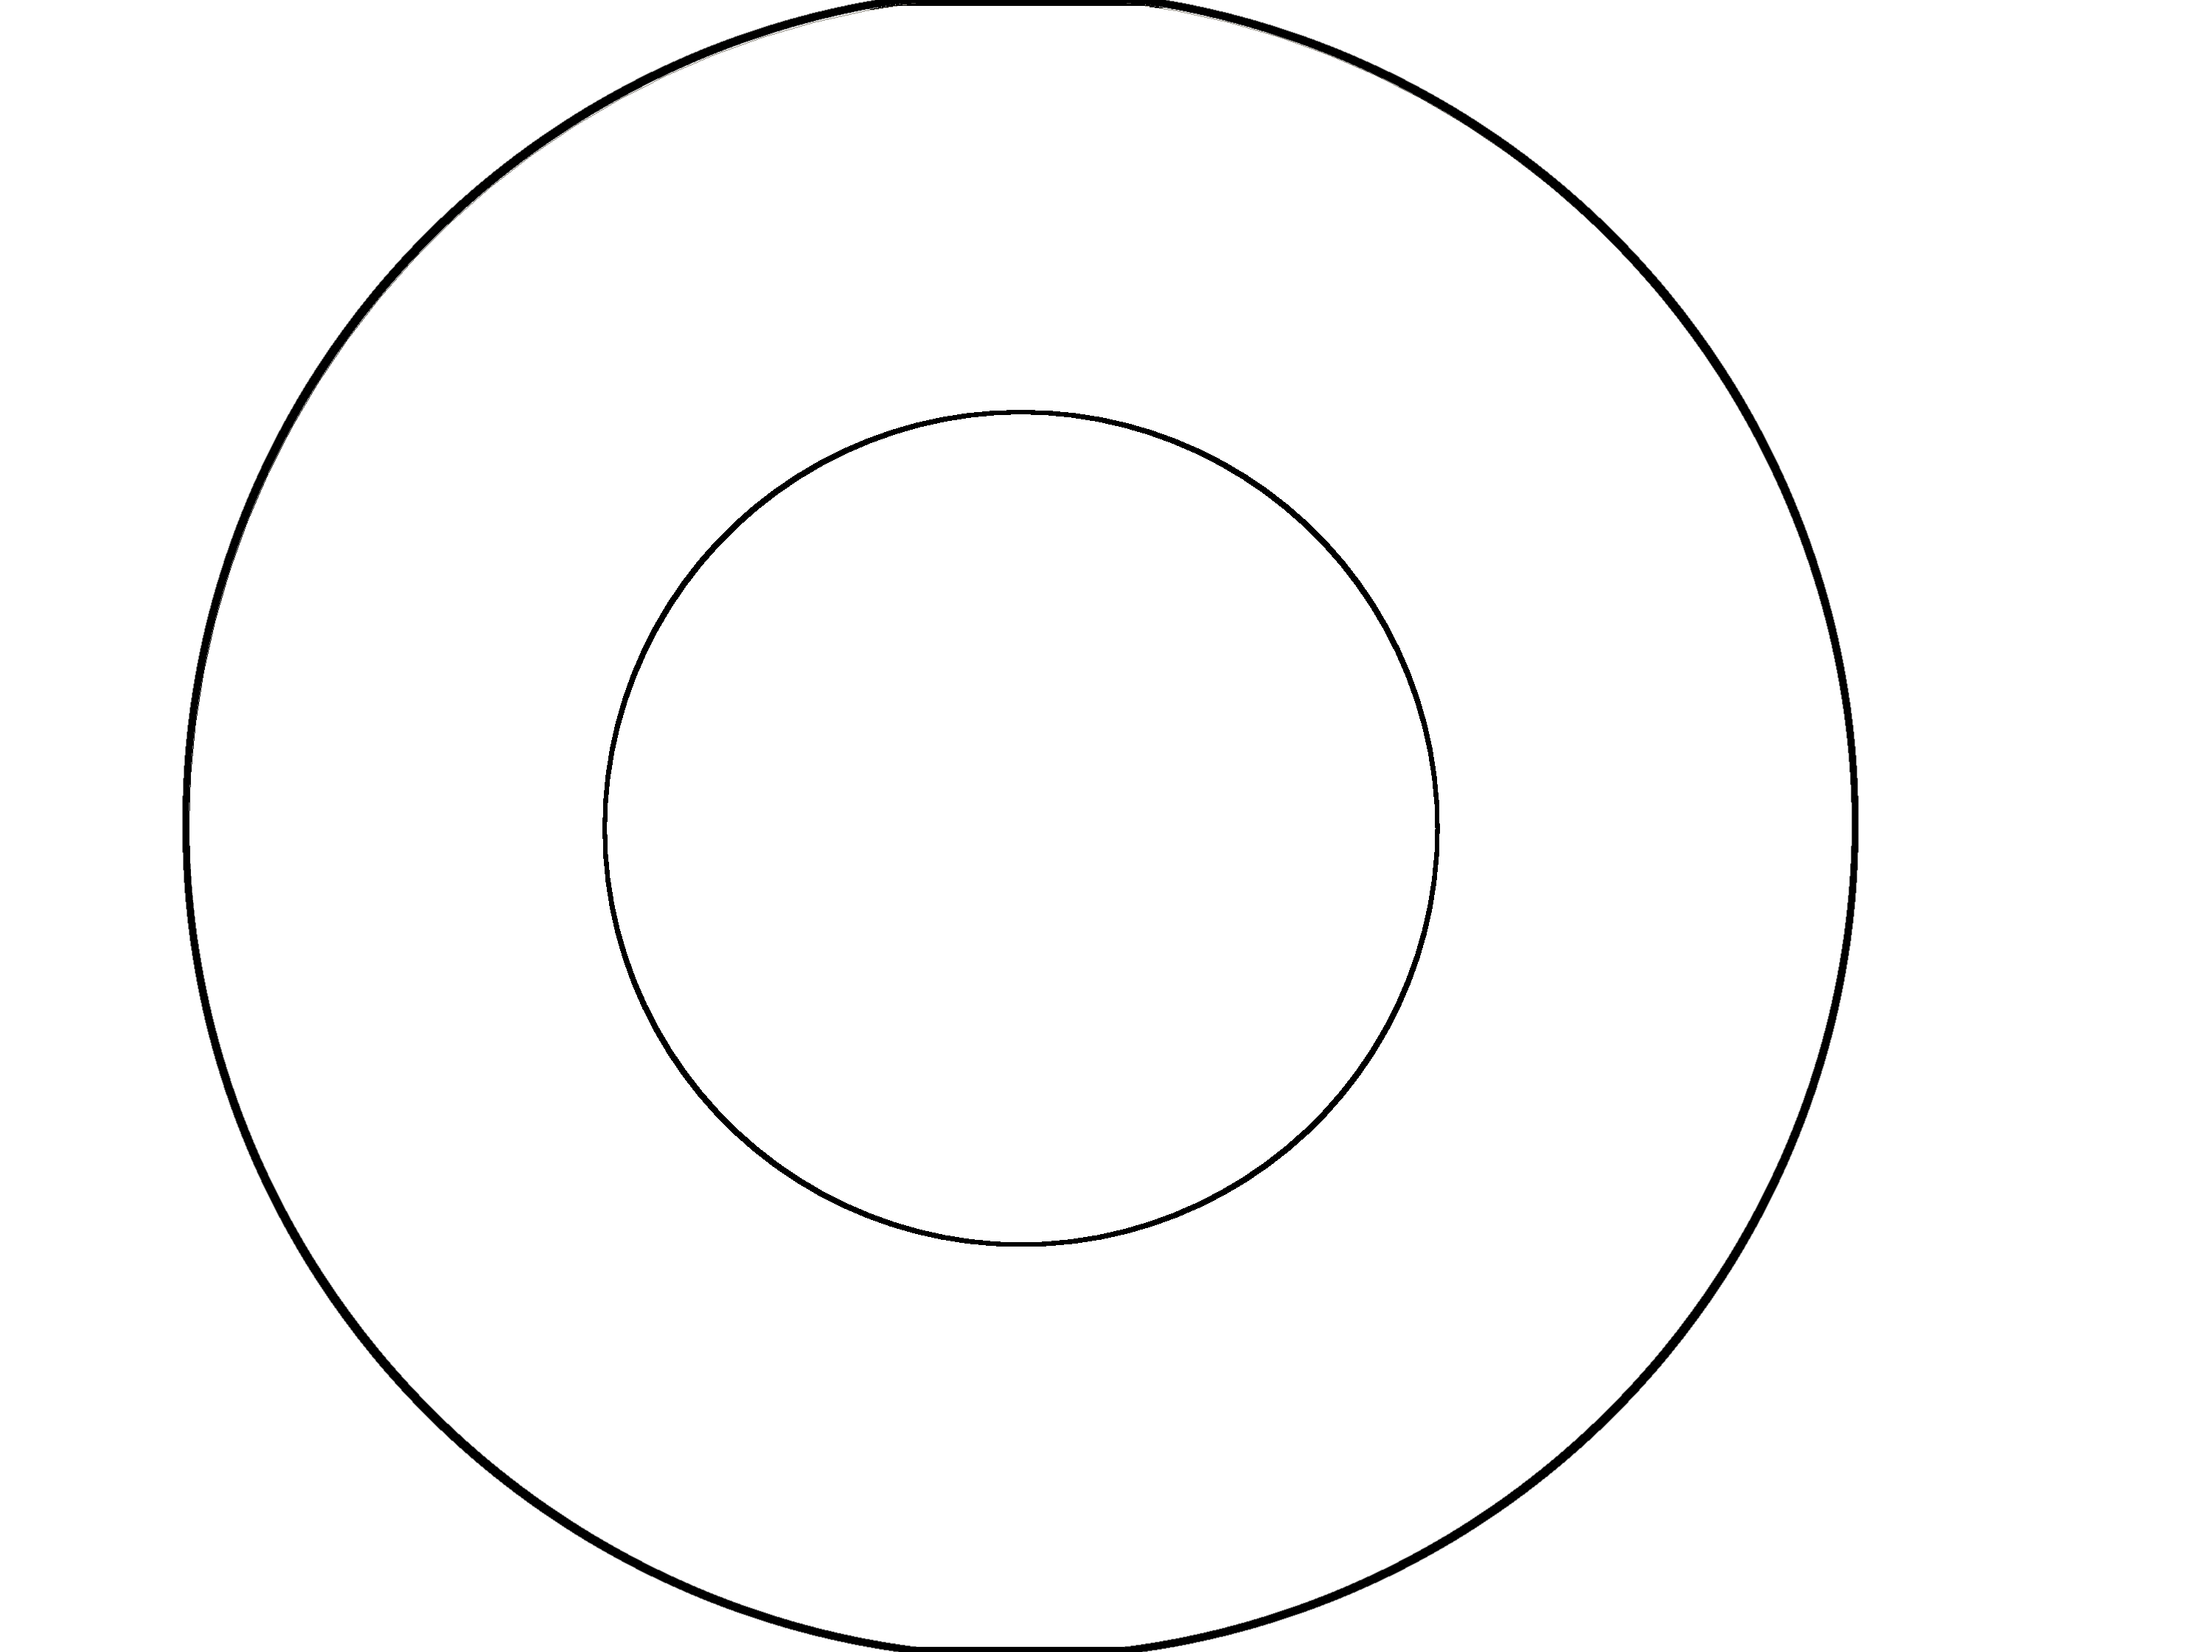
\includegraphics[width =0.35\textwidth]{figs/forcing_region}
     \caption{An example of explicitly represented turning vanes (left)
    versus an annular forcing region (right).}
     \label{fig:penalty_model}
   \end{figure}

Vane geometry is specified by the angle $\phi$ a vane makes with a
radial line as a function of the radial coordinate, $r$, and the polar
angle, $\theta$. A unit normal to the vane surface ${\bf n_v}$ is defined
as 
%
\begin{equation}
 {\bf n_v}({\bf x}) = \sin \left(\phi(r,\theta) \right) \hat{{\bf r}}+ \cos
  \left(\phi(r,\theta) \right) \hat{{\bf \theta}} 
\end{equation}
%
where $\hat{{\bf r}}$ and $\hat{{\bf \theta}}$ are unit
vectors in the radial and azimuthal directions, respectively.
With this vane-normal vector field specified, a body force ${\bf f_v}$
is defined that will drive the velocity in the ${\bf n}$ direction
toward zero, effectively turning the flow to be parallel to the
vanes. The body force is defined by,
\begin{equation}
 {\bf f}_v= -\frac{1}{\ell_v}|{\bf u}|({\bf u}\cdot{\bf n_v}){\bf n_v}
 \label{eqn:body_force}
\end{equation}
with ${\bf u}$ the velocity and $\ell_v$ is a specified length
scale. $\ell_v$ represents the distance over which the
flow evolves under the influence of the body force before the
velocity in the normal direction is reduced by a factor of $1/{\bf 
e}$.
That is, this is the length over which the normal component of the
velocity decays exponentially. 
%It is the distance analog to the more
%familiar time constant of exponential decay. 

Therefore, $\ell_v$ is a modeling constant and must be specified. Our
expectation is that it will be the same order as the separation distance
between neighboring vanes in the physical vane configuration, since
entry  lengths in internal flows scale with the width of the
channel. This study\todo{what study, describe what i did} is depicted in
Figure~\ref{fig:annealing}, where the average misfit between the turning
vane angle in an explicitly represented vane configuration and the flow is plotted.   

The trend is clear that as the flow moves through the turning vanes
towards the center of the apparatus it is brought into alignment with
the turning vane direction. 
Notice that the misfit actually grows near the minimum, likely due to
unmodeled transient effects such as vortex shedding off the vane
trailing edges. 

   \begin{figure}[!htb]
    \centering
    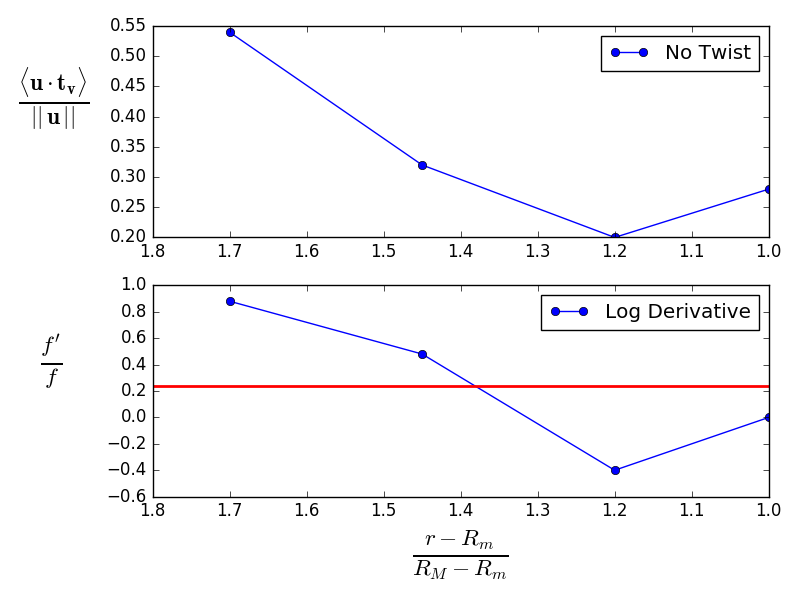
\includegraphics[width =0.8\textwidth]{figs/annealing}
     \caption{The average misfit between the gridded vanes and the
    flow. The averaging is accomplished through azimuthal
    averaging. This was taken at half the height of the turning vanes,
    although the results do not differ at greater or lower height. 
    The subfigure shows the logarithmic derivative, as well as the
    average of the logarithmic derivative in red. 
$R_{M}$ is the furthest radial extent of the gridded vanes,
    and $R_{m}$ the smallest radial extent. The subfigure shows the
    logarithmic derivative of this quantity.}
     \label{fig:annealing}
   \end{figure}


Now, $\ell_v$ can be calibrated to explicitly match the results of the
gridded vanes by assuming that the vane mismatch obeys a radial
exponential decay of the form $f(r) = A e^{-\ell_v r}$, and taking the
logarithmic derivative of this quantity, 
\begin{eqnarray}
 \frac{f'}{f} = \frac{A e^{-\ell_v r} * -\ell_v}{A e^{-\ell_v r}} =
  -\ell_v. 
\end{eqnarray}

This is shown in subfigure of Figure~\ref{fig:annealing}, where we would
expect a flat line if the misfit between vanes was perfectly described
by an exponential decay. While the curve does not perfectly coincide
with this, the curve does not have severe convexity and the average is
sufficient for this work. Based on this, the lengthscale $\ell_v$ was
set to three\todo{what? it has dimension}. 

%\todo{show
%calibration of this} 

This virtual vane formulation is similar to the ``actuator disk'' model
commonly used to represent the rotor of a wind turbine and
described in the subsequent section. 

\section{Turbine Representation}
\label{sec:actuator_disk}
%
% https://en.wikipedia.org/wiki/Blade_solidity
%

The turbine is modeled similarly to the virtual vanes. As with the
vanes, it is desirable to avoid explicitly representing the turbine
blade control surfaces. Instead, the turbine is modeled using the
actuator disc simplification. 
This model (also often referred to as a ``Blade Element Momentum''
theory) is commonly used in wind
turbine design\cite{shevell1983fundamentals,betz,leclerc}. The essence
of this model is to approximate the individual spinning turbine blades
as a ``disk'' in which the effects of the turbine are represented by
body forces on the fluid, as shown in Figure~\ref{fig:actuator_disk}.
This method assumes an axisymmetric representation of the turbine
geometry, and in doing so completely neglects unsteady effects due to
the rotation of turbine blades in a plane. 

As the flow moves through the actuator disk, it experiences a force
normal to the represented turbine blade surface. This force will
generally be in opposition to the flow direction, and will therefore
impart a loss of momentum on the fluid. 
Associated with the loss of axial and azimuthal momentum is a loss of
energy which can be collected by an electrical generator attached
to the rotor shaft if the rotor experiences a torque
in the direction of rotation. 

All the turbine cases shown in this study make the further
simplification that the rotation speed of the disk is constant. 
In this way it is assumed that the turbine exerts a torque equal and
opposite to that of the airflow which keeps the rotational speed
constant. The work done by the aerodynamic torque on the
turbine is assumed to feed into a generator, where it is converted into
electrical energy. 


   \begin{figure}[!htb]
    \centering
    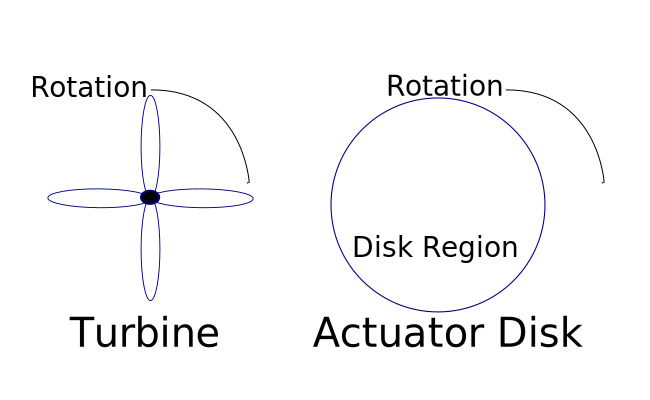
\includegraphics[width =0.95\textwidth]{figs/actuator_disk}
     \caption{The actuator disk model represents a turbine blade
    geometry (shown on the left) as a spinning ``disk'' region (shown
    on the right).}
     \label{fig:actuator_disk}
   \end{figure}

We now detail the mathematical machinery necessary to specify the
direction and magnitude of force between the turbine and flow. The
normal in the blade's velocity direction is, 
\begin{equation*}
n_B = \frac{{\bf u_B}}{||{\bf u_B}||}. 
\end{equation*}
Where ${\bf u_B}$ is the blade velocity vector and is specified. The
normal in the fan vertical direction is typically ${\bf n_f} =
\left(0,0,1\right)$, e.g. pointing ``up''. Then the normal in the radial
direction must be,  
\begin{equation*}
{\bf n_r} = {\bf n_B} \times {\bf n_f}
\end{equation*}

% The fan-wing-plane bit means that we're only looking at the projection
% of velocity into the plane that's defined by the base velocity and
% vertical direction. 

% (01:03:44 PM) Roy Stogner: The "local relative velocity" means that
% we're taking the velocity not in the reference frame of the domain, but
% in the reference frame of the wing.  So if the base velocity is U_B and
% the air velocity is U, then the local relative velocity is U - U_B. 
% (01:04:25 PM) Roy Stogner: Note that we simplify that equation a tiny
% bit by using the fact that U_B and N_R are perpendicular. 

and the fan-wing-plane component (e.g. the plane perpendicular to the 
radius) of local relative velocity is
\begin{equation}
{\bf u_p} = {\bf u} - ({\bf u}\cdot {\bf n_r})\cdot {\bf n_r} - {\bf u_B}. 
\end{equation}
This is the projection of velocity into the plane defined by the base
velocity and vertical direction. Now the ``forward velocity'' in the
reference frame of the turbine is,  
\begin{equation}
{\bf u_{\text{fwd}}}= -{\bf u_p} \cdot {\bf n_B}
\end{equation}
and the ``upward'' velocity in this frame is, 
\begin{equation}
{\bf u_{\text{up}}} = {\bf u_p} \cdot {\bf n_f}. 
\end{equation}
The angle with respect to the fan velocity direction is then, 
\begin{equation}
 \theta_f = \text{atan2}\left(\frac{{\bf u_{\text{up}}}}{{\bf u_{\text{fwd}}}}\right)
 %\theta_f =
  %\text{tan}^{-1}\left(\frac{u_{\text{up}}}{u_{\text{fwd}}}\right)
  \label{eq:fan_direction}
\end{equation}
while the angle with respect to the chord is this with the addition of
the blade angle relative to the fan vertical direction, 
\begin{equation}
 \phi = \theta_f + \beta(r).
\end{equation}

In words, the blade angle (or local pitch) is measured from the plane of
rotation to the chord line (i.e., the straight line connecting leading
to trailing edge). These parameters, $\beta$, C, etc. are visually
depicted in Figure \ref{fig:turbine_image}.  

The actuator disk model assumes that the forces on a blade
element can be calculated by means of two-dimensional aerofoil
characteristics using an angle of attack determined from the incident
resultant velocity in the cross-sectional plane of the element. The
velocity component in the span-wise direction is
ignored. Three-dimensional effects are also
ignored\cite{burton2001wind}.  

  \begin{figure}[!htb]
    \begin{center}
     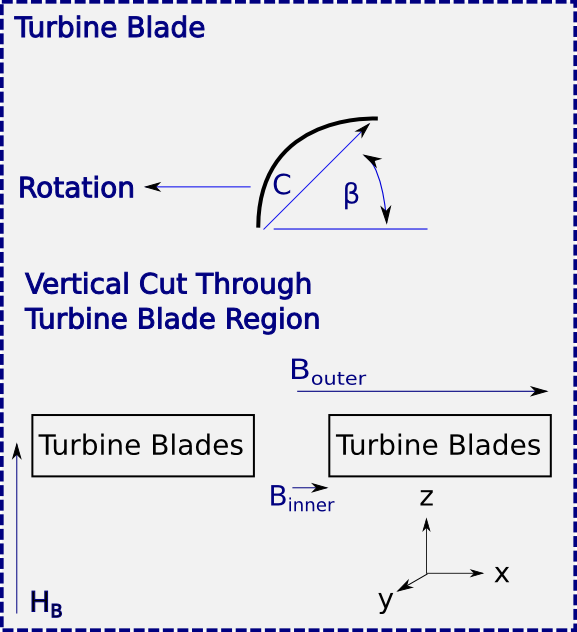
\includegraphics[width = 10 cm]{figs/turbine_image}
     \caption{The represented turbine blade
     geometry. $\beta$, the blade angle, is measured relative to the
     horizontal plane. c, the chord length of the turbine, is defined as
     the straight line distance from leading to trailing edge. } 
     \label{fig:turbine_image}
    \end{center}
  \end{figure}

\subsection{Drag Polar Specification}

We now define the lift and drag normals, where the direction opposing
drag is, by definition,  
\begin{equation}
{\bf n_{\text{drag}}} = \frac{{\bf u_p}}{||{\bf u_p}||} 
\end{equation}
and the direction opposing lift orthogonal to the drag and the radial 
direction,  
\begin{equation}
{\bf n_{\text{lift}}}= {\bf n_{\text{drag}}} \times {\bf n_r}. 
\end{equation}

Then, the force on the turbine is, 
% \begin{equation}
%  \boxed{F = \frac{1}{2}\frac{\rho u_p^2 c}{A}\left(C_l \cdot
% 					      n_\text{lift} + C_d \cdot
% 					      n_\text{drag}  \right)}
% \label{eq:force_turb}
  % \end{equation}
\begin{equation}
 F = \frac{1}{2} \rho A_B {\bf u_p}^2 \left(C_l 
					      {\bf n_\text{lift}} + C_d 
					      {\bf n_\text{drag}}  \right).
\label{eq:force_turb}
\end{equation}
$A_B$ is the total area of the turbine blades, so $A_B = B\, c\, r$, where B
is the number of turbine blades and c is the chord length of the
turbine. 
The actuator disk is an approximation of the blades as a volumetric
forcing ``disk'', and so our interest is in this quantity,
\begin{equation}
\frac{F}{\text{volume}} = \frac{F}{\pi r^2 t} = \frac{1}{2}\frac{\rho\, B\, c\,
 {\bf u_p}^2}{\pi r t}\left(C_l {\bf n_\text{lift}} + C_d {\bf
		   n_\text{drag}} \right).  
\label{eq:vol_turb}
\end{equation}
Where t is the blade thickness of the actuator disk.
Note that the volume is over a different extent than the area. The
volume is for the entire actuator disk, while the force on the blades
was only calculated with total surface area of the turbine. 
To better understand this, note that the product, $B c$ appears in
Equation~\ref{eq:vol_turb}, above. This quantity is a solidity (or
blockage) factor, and as the chord length or number of blades increases,
the total blocked area inside the actuator disk also increases. It is
interesting to note that in the actuator disk model, only this product
has impact, and one cannot directly separate the impact of more turbine
blades versus larger blade chord lengths. 
The impact of solidity will be discussed in greater detail in
Section~\ref{sec:solidity}.

Now, only the drag polars ($C_l,C_d$) must be specified to fully
determine the force on the blades. These drag polars are functions of
the angle of attack, $\alpha$. Plots of these drag polars were provided
by Duane McCormick at UTRC and were generated from a 2-D model in
COMSOL. As the data was discrete, high order polynomials were used
to obtain smooth functions fit to the COMSOL data. Typically,
16\textsuperscript{th} order polynomials were used to 
ensure that the fitted function closely matched the provided
data. The drag and lift functions for the three cases considered (flat
plates, $180^{\circ}$, $90^{\circ}$ circles) are shown in 
Figures~\ref{fig:flat_plate_drag}, \ref{fig:semi_drag} and
\ref{fig:90_drag}. The flat plate drag polars are smoothly
varying and so the interpolated function is close to the provided
data. The semi-circles ($180^{\circ}$) are largely accurate, but near
zero degrees the COMSOL data for the lift function shows a sharp feature
that is not well resolved by the interpolating polynomial. This is also
the case for the quarter-circles, where near a zero angle of attack the
lift function has a near discontinuity that is not well resolved by the
interpolated function. 

%The semi-circular plots are more complicated. Here, we use a high order
%polynomial fit to continuously interpolate between drag polars. 

\begin{figure}[!htb]
  \begin{center}
    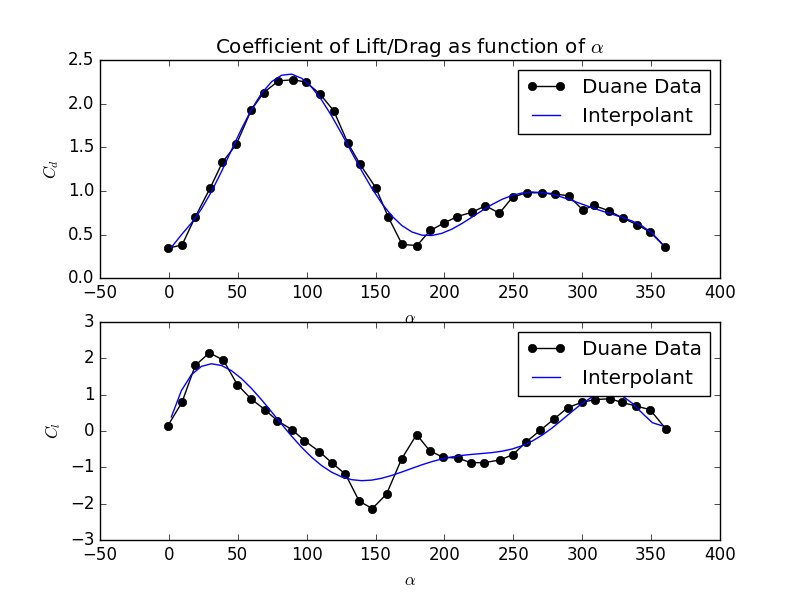
\includegraphics[width = 12 cm]{figs/flat}
    \caption{The flat plate drag polars.} 
    \label{fig:flat_plate_drag}
  \end{center}
\end{figure}

\begin{figure}[!htb]
  \begin{center}
    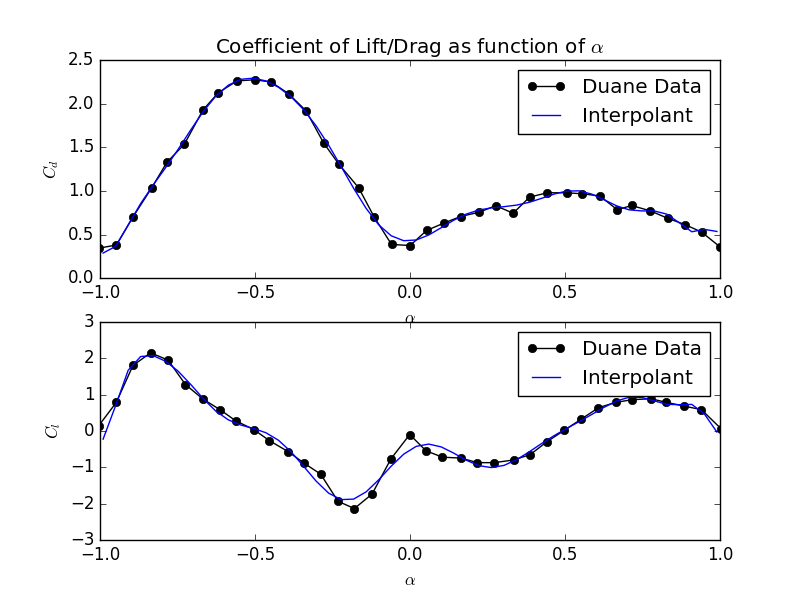
\includegraphics[width = 12 cm]{figs/semi}
    \caption{The semicircle (180 degree) drag polars.} 
    \label{fig:semi_drag}
  \end{center}
\end{figure}

\begin{figure}[!htb]
  \begin{center}
    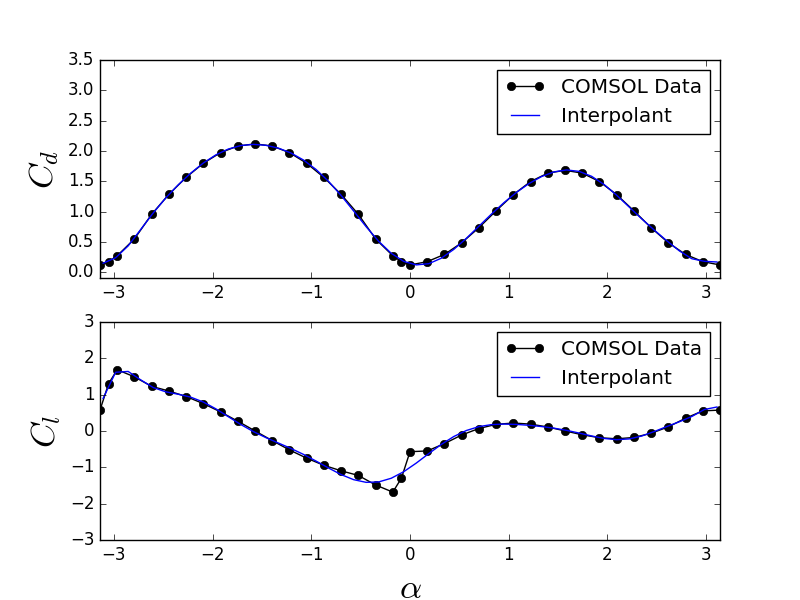
\includegraphics[width = 12 cm]{figs/90}
    \caption{The 90 degree drag polars.} 
    \label{fig:90_drag}
  \end{center}
\end{figure}

% what about loads on turbine?\todo{loads?}
% Blade torque loads modest, only ~20 ft-lbs
%% load was predicted at 20 ft*lbs

\subsection{Shortcomings of the Actuator Disk Model}
\label{subsec:wake_loss_model}

The actuator disk model is valuable because of its simplicity, not on
account of its accuracy. Despite its pervasive use, there are numerous
known inadequacies to the model. 

In particular, the actuator disk does not account for the separation of
flow between blades, and implicitly assumes the flow remains attached. 
This model deficiency results due to the actuator disk
method's dependence on the precision of the lift and drag
coefficients. During the operation of a wind turbine, should the angle
of attack reach high values (post-stall region), then aerodynamic
data is not available or inaccurate.  
This model inadequacy is commonly fixed with the Glauert Correction. 
Developed in 1926 by Glauert from helicopters rotor blades, this
correction originally was purely based on experimental data. The model
was designed to correct the overall thrust coefficient for high angles
of attack\cite{glauert1926general,glauert1935airplane}. 
While the Glauert correction is a tip loss model, the correction was
developed as a correction to an entire rotor disk; the original
researcher did not intend it to be applied to a rotor annulus. 
%Given that 
%a duct eliminates tip losses\todo{write me}
%However, because of a limited amount of experimental data, an alternative model does not exist.  

Nor do the model's described above account for the turbulent wake
state, which in some cases have been shown to be significant for a wind
turbine\cite{churchfield2012numerical} and may have substantial impact
on the SoV. 

Various researchers\cite{Moriarty_aerodyntheory,wilson1978design} have
suggested various other corrections to actuator-disk theory. These
corrections include (among others) accounting for blade thickness on
local angle of attack, cascade width for high solidity turbines, and
spanwise gaps for partial span pitch control. The impact of these
missing physics can be significant, for instance, blade thickness and
effects can be aerodynamically significant near the rotor hub and may 
affect the in-plane forces on the rotor. Nevertheless,
these corrections are not treated in the simulations presented in this
document. 

In summary, the actuator disk is a useful modeling tool for this study
but does not represent a high-fidelity representation of the turbine
blade dynamics, and should not be considered highly accurate. Attempts
to evaluate and characterize these shortcomings are detailed in
Chapter~\ref{sec:field}.  Additionally, a new modification to the
actuator disk that modifies the model to further account for blade
solidity is demonstrated in this work in Section~\ref{sec:solidity}. 

\section{Solid Surface Representation}
\label{subsec:solid_surface}

In addition to vanes, the SoV device includes impermeable surfaces
such as the wind break (``cone'') on the top of the facility. As with
the turning vanes, this is represented without explicitly meshing the
surface nor imposing  a boundary condition at the surface. This allows
rapid exploration of configurations  with different solid surfaces to
control and manipulate the fluid flow. These solid surfaces are
represented by a body force acting in a region surrounding the wall. 
A body force normal to the surface is defined in this region so
that it will drive the normal velocity to zero, resulting in the flow
moving only parallel to the virtual surface. 
The body force is defined as in Equation
\ref{eqn:body_force}; however, the length scale $\ell_v$ is specified to
be identical to the width of the surface being represented. This is
typically the width of two or three grid cells. While the actual surface we are
emulating is thinner than this, the numerical method has difficulty
converging for surfaces smaller than the grid size.  

Forcing models designed to mimic a surface
are not unique to this project, and the current formulation is
 closely related to (among others)
``immersed boundary methods'' as used by various other
researchers~\cite{doi:10.1146/annurev.fluid.37.061903.175743,verzicco1998complex}. This
approach is unique in its use of Babuska's penalty treatment of
constraints\cite{1973fempen,ZAMM:ZAMM19880680925} to enforce the
behavior at the boundary. This method was selected because it is easily
imposed in the FEM context, and the penalty method proper has been
explored in detail in the literature.
%\todo{add more discussion of
%healing length implications here} 

Note that despite the similarity in name, this is a distinct technique
from the ``penalty immersed boundary method'' of Kim and
Peskin\cite{:/content/aip/journal/pof2/19/5/10.1063/1.2734674}.  

%show image of cylinder in 2d flow?\todo{add cylinder image? what does
%zthis show?} 

%Typically, the enforcement occurs along a domain
%boundary, but in this work it is used in the interior, 
%and is not imposed as a mathematical constraint but rather as a modeling 
%approach. 

% We add a penalty term to the weak
% form of the Navier-Stokes momentum equation described in the subsequent
% section %\ref{eq:ns_weak} 
% that has the form, 
% \begin{equation}
% P_\epsilon = \int_\Omega ({\bf f_v} \cdot v) \, dx
% \end{equation}
% where ${\bf f_v}$ is as described in equation \ref{eqn:body_force}. 
%% As the system is formulated as a variational problem that seeks to
%% minimize the test function $v$, any velocity that is not aligned with
%% the vane normal will incur a penalty versus one that does. Note that unlike
%% some penalty methods, this does not automatically satisfy
%% continuity. Rather, the velocity field remains divergence free through a
%% separately enforced constraint.  

\section{Separation Model}
\label{sec:separation}

In the presence of wind, it was found that there was a significant flow
out through the vanes in the back of the device. This was obviously
inconsistent with the findings of our colleagues in the field, who
observed no outflows out of the back of the device. Moreover, this resulted
in large inconsistencies between our predictions and the field results,
almost certainly because of the kinetic and thermal energy that our vane
representation was permitting to leave out the back of the device.  

This exposed a weakness of the turning vane representation outlined
previously. When the flow entered the virtual vane forcing region it was
always turned to align with the vane angle, even when the forcing was in
the opposite direction of the present velocity.
This is in contrast to the physical situation, in which we
expect the flow to continue along an averaged streamline separating from the 
trailing edges of the vanes, instead of turning around it. 
The averaged streamline will continue past the trailing edge of the vane
due to the separation of the boundary layer off the edge surface. An
image depicting these two cases in shown in Figure \ref{fig:sep_model}.  

\begin{figure}[!htb]
  \begin{center}
    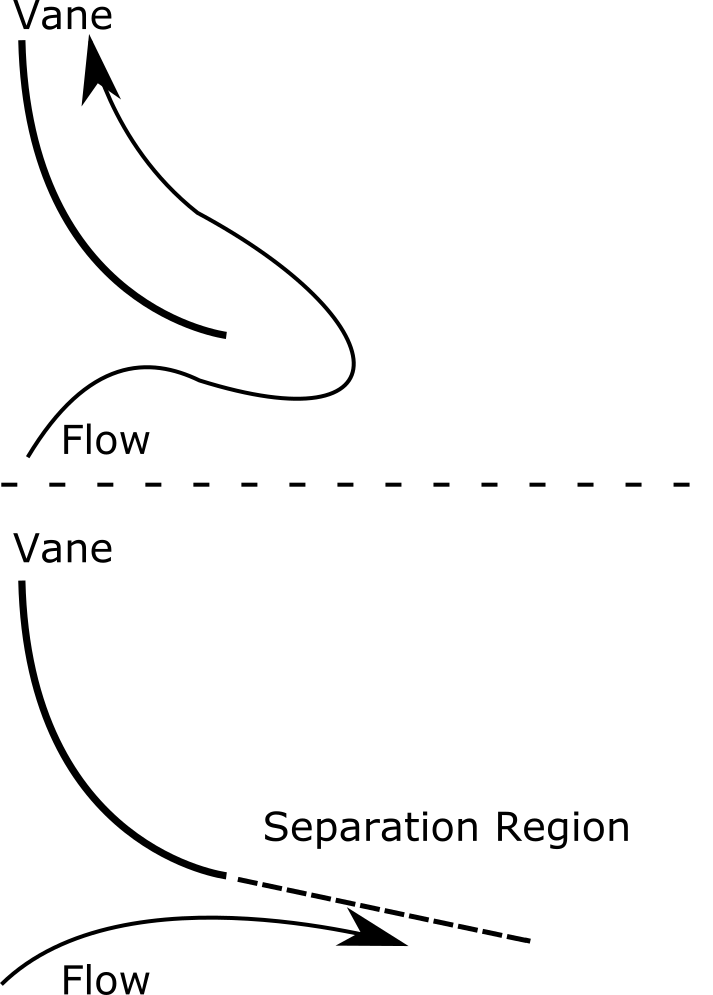
\includegraphics[width = 6 cm]{figs/sep_model}
    \caption{Schematic depicting the separation model that extends past
   the trailing edge of the vanes. In the top case, the flow entering
   the virtual vane region is forced to align with the vane angle despite
   this resulting in a reversal of the flow direction. This is a
   consequence of the forcing function acting on the fluid to ensure the
   velocity vector aligns with the vane. 
   The second case depicts the separation
   model, where the flow under certain conditions is not forced and
   continues to move tangent to the vanes due to 
   the separation of the boundary layer off the trailing edge.} 
    \label{fig:sep_model}
  \end{center}
\end{figure}

Let $\bf n_v$ be the normal vector to the vanes,
and $\bf n_r$ the normal vector pointing out of the vane
region\footnote{\normalsize The subscripts ``v'' and ``r'' stand for
vane and radial, respectively.}.  
Then, $\bf t_v$ is the tangential vector to the vanes pointing out of
the vane region and is defined as,

%\begin{equation}
% \bf t^v = \left( {\bf n^v_y},{\bf -n_x^v} \right) \text{sign}\left[
%	    \left( {\bf n^v_y},{\bf -n_x^v} \right) \cdot {\bf n^r} \right].
%\end{equation}
\begin{equation}
 \bf t_v = \left( {\bf n_v^{\perp}} \right) \text{sign}\left(
	    {\bf n_v^{\perp}} \cdot {\bf n_r} \right).
\end{equation}
Here, ${\bf n_v^{\perp}}$ is the vector perpendicular to the normal
vector of the vanes, which is simply, 
\begin{equation*}
 {\bf n_v^{\perp}} = \left[ \begin{array}{c}
n_x\\
n_y\\
\end{array}\right]^{\perp} = 
 \left[ \begin{array}{c}
  -n_y\\
  n_x\\
	\end{array}\right].
\end{equation*}

%
% example of an algorithm
%

\begin{center}
 \begin{algorithm}
  \caption{The crude separation model. This model identifies if the flow
  is coming into or out of the vane region, and if the velocity vector
  is in the same direction as the tangent line of the vanes. In the case
  of the ``special forcing'' the flow is forced as if it was
  impacting a solid surface. In the
  algorithm below, $r_0$ is the max radius of vanes, $r_i$ the minimum
  radius of vanes, and $\delta$ is the width of the separation region.}
  \label{alg:sep}
  \begin{algorithmic}
   \IF{($r_0 > r > r_i$)} 
   \IF{$(r_0 - r) < \delta$ \textbf{or} $((r - r_i) < \delta)$}
   \STATE ${\bf n_r} = {\bf r}/|r|$
   \IF{$(r - r_i) < \delta$} 
   \STATE ${\bf n_r} = -{\bf n_r}$
   \ENDIF
   \STATE  $\bf t_v = \left( {\bf n_v^{\perp}} \right) \text{sign}\left(
  	    {\bf n_v^{\perp}} \cdot {\bf n_r} \right)$
   \IF{$v \cdot t_v > 0$ \textbf{and} $v \cdot n_r < 0 $}
   \STATE ${\bf n}({\bf x}) = \hat r$ \quad (Special Forcing)
   \ELSE
   \STATE  ${\bf n}({\bf x}) = \sin \left(\phi(r) \right) \hat{{\bf r}}+ \cos
  \left(\phi(r) \right) \hat{{\bf \theta}} $
  \quad (Normal Forcing)
   \ENDIF
   \ELSE
   \STATE ${\bf n}({\bf x}) = \sin \left(\phi(r) \right) \hat{{\bf r}}+ \cos
  \left(\phi(r) \right) \hat{{\bf \theta}} $
  \quad (Normal Forcing)
   \ENDIF
   \ENDIF
  \end{algorithmic}
 \end{algorithm}
\end{center}


The forcing is modified when the velocity vector of the local flow, $\bf
u$ is pointing in to the forcing region: ${\bf u} \cdot {\bf n_r} < 0$, and
when the velocity vector is in the same direction as the tangent line to
the vanes: ${\bf u} \cdot {\bf t_v} > 0 $. In these instances, the
forcing acts as if there was a rigid surface past the vane edge, and
gives the appearance of a special ``no-penetration'' condition for the
velocity for these cases. The pseudo-code for this procedure is shown in
Algorithm~\ref{alg:sep}.

The addition of this simple separation model significantly reduced the
flow that penetrated the back of the vanes, and produces results
consistent with the observations provided by our experimental
colleagues.  

\section{Effect of Surface Roughness}

%%
%% this does not describe the phenomena being modeled or the precise
%% model -- rewrite
%%
%%
%% this does not say enough about the surface roughness
%% motivate that and explain how it is used, than show your estimate 
%% to argue it is small
%%

Surface roughness effects have been shown to play a role in the
formation of dust devils and related atmospheric
phenomena\cite{oke1987boundary}. For the flat and sandy
regions we are simulating, the impact is expected to be a small
``kick-up'' forcing velocity perturbation in the vertical
direction. Assuming azimuthal symmetry and forcing only inside the
region of the vanes ($r<R$), this is modeled as a volumetric forcing in
a narrow region above the surface,  
\begin{equation}
 F^{'''}_{z_0} = \frac{1}{2}\rho V_f^2/z_{0}, 
\end{equation}
where $z_{0}$ is the roughness height. We further assume that this
forcing is independent of ${\bf u}$. To estimate the magnitude of
$V_f$, we use a simple result from Newton's laws of motion,
\begin{eqnarray}
z_0 = \frac{1}{2} a t^2, \\
t = \sqrt{\frac{2 a}{z_0}}. \\
\end{eqnarray}
Combining this with, $V_f = a t$, our estimate is, 
\begin{equation}
V_f = \sqrt{2 a z_0}.
\end{equation}
The roughness height zero is set to the boundary layer thickness of 10
centimeters. The acceleration was estimated at 0.05
$\text{m}/\text{s}^2$, based on the observed surface roughness impact on
tornado-like vorticies of Natarajan and Hangan\cite{Natarajan2012577}.  

We ensure that the energy
introduced into the flow is a small fraction of total flow energy by comparing
this with the energy flux through the top of the vanes. The total energy
added is measured as,  
\begin{equation}
 E_{\text{injected}} = \int_0^{2\pi} \int_0^R \int_0^{z_0} F^{'''}_{z_0}
  dz dr d\theta.  
\end{equation}
R is the outer diameter of the vanes. 
The value of $E_{\text{injected}}$ is typically a few percent of the
total kinetic energy flux measured through the top of the
vanes.

Leslie~\cite{leslie1977surface} and Dessens~\cite{dessens1972influence}
found that the introduction of surface roughness effects caused a slight
decrease in tangential velocity for simulated vortices, but an increase
in radial and axial velocities. 
On a related note, hurricane studies have
consistently found enhanced heat transport near the surface lead
to storm intensification, indicating an important role due to roughness
effects~\cite{Zeng2010,GRL:GRL50047,hurricane_drag}. The interaction
with the surface and therefore, the impact of roughness, is likely
complicated and is not considered in detail in this work. It should be 
noted that in the simulations performed in the course of this study, the
surface roughness model was observed to modestly intensify the thermal
vortex, typically by several percent. While this formulation was
undoubtedly {\it ad hoc}, studies performed on representative test 
cases found that results were not sensitive to small
changes in the forcing region height, radial distance, or
forcing magnitude. 

%This general forcing provides additional capabilities including the
%ability to investigate engineering greater surface roughness or
%structures that could provide greater ``kick-up'' of the thin thermal
%layer near the surface into the flowing regime. It can also support more
%general turning configurations than the virtual vanes outlined above. 

\section{Simulation Geometry and Boundary Conditions}
\label{sec:bc}

In this project, two principle modeling regimes are considered.  
One is the ``thermal-only'' scenario, in which there are no ambient
velocities and there is an imposed elevated temperature on the ground.  
In the other, there are also ambient winds that contribute to the SoV energy
(``wind'' cases). 
The computational domain and boundary conditions for these 
two scenarios are described below.

%\subsection{Computational Domain} 
\textbf{Computational Domain} 

All simulations are performed in a cuboid domain, with six
faces.  The domain is denoted $\Omega \subset \mathbb{R}^3$. 
The domain extents are scaled by the system diameter, D, created by the
outer vane radius. The extents are defined in terms of $\{L_x,L_y,L_z\}$ indicating the 
streamwise, spanwise and vertical directions, respectively. 
For both simulation regimes, sensitivity analyses 
were performed to ensure that the results were not sensitive 
to the domain extents. For the thermal-only case, for which $L_x = L_y$,
the system 
extents $L_x/D$ and $L_y/D$ are chosen to be 3. The height ($L_z/D$) is
three times the system diameter, which is typically nearly equal to the
height of the vanes. This defines the thermal-only domain $\Omega_T$, 
as $\Omega_T = \left[-L_x,L_x \right] \times \left[-L_y,L_y \right]
\times \left[0,L_z \right]$.   

For the wind cases, the streamwise extent is no longer equal to
the spanwise length, $L_y$. In these cases, the domain length extends
two diameters in front of the vanes and three behind. The
spanwise direction is symmetric and extends two diameters in each direction 
from the center ($L_y/D = 2$). The height is identical to the
thermal-only case, at three system diameters ($L_z/D = 3$). Thus, the
wind domain is defined as $\Omega_W = \left[-2D,3D \right] \times
\left[-L_y,L_y \right] \times \left[0,L_z \right]$.   

The boundary for the thermal only case is decomposed as,
$\partial \Omega_T = \Gamma_G \, \bigcup \, \Gamma_T \, \bigcup \, \Gamma_P $. 
$\Gamma_G$ is the boundary along the ``Ground'', $\Gamma_T$
the ``Top'' boundary, and $\Gamma_P$ the four periodic ``Sides''. A 3d
diagram labeling these boundaries is shown in
Figure~\ref{fig:thermal3d}. For this case study (no mean wind),
periodic boundary conditions are used on the four sides , with a modified 
``inflow-outflow'' Neumann condition\cite{gunzburger1989finite} on the
top boundary. On the ground, a ``no-slip'' velocity boundary condition is
imposed, and a Dirichlet condition uniformly fixes
the temperature of the surface. 
Each of the $\Gamma$ boundary terms are defined in the paragraphs below. 
Note that a finite thickness ``Sponge Layer'' is
indicated on the figure along the top boundary and is defined below. 

\begin{figure}[!htb]
  \begin{center}
    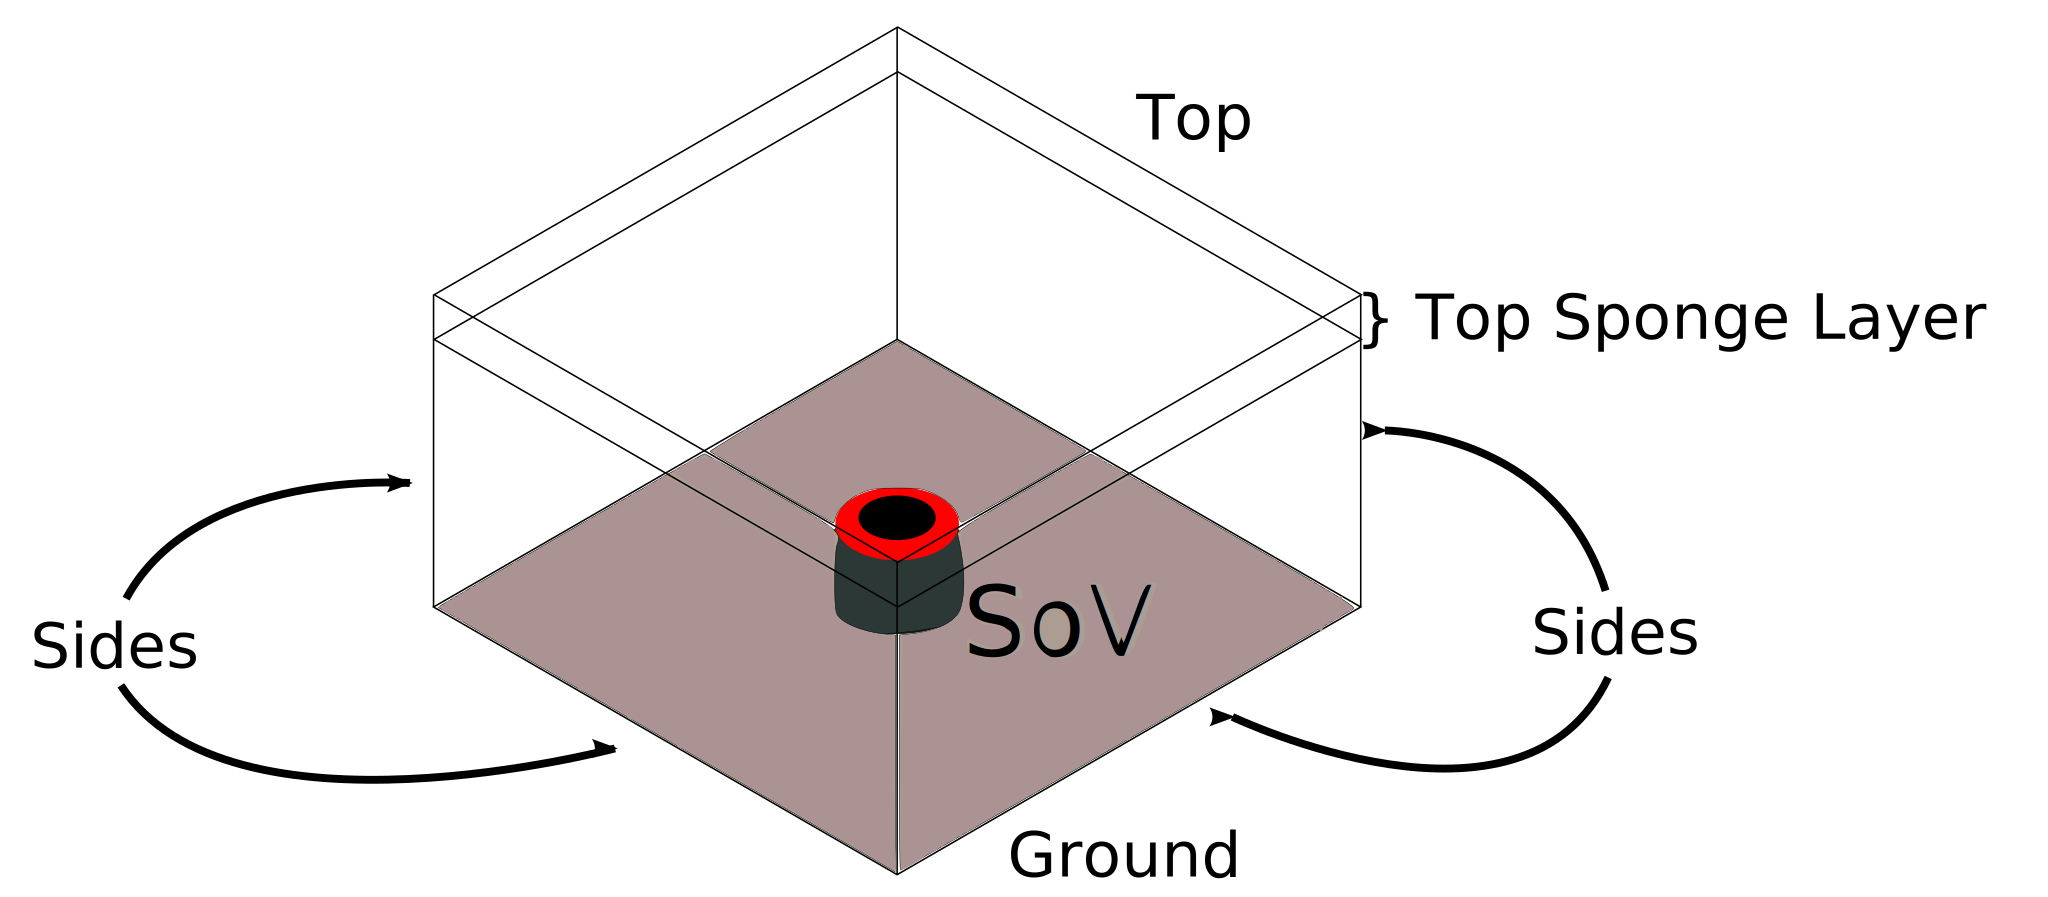
\includegraphics[width=14cm]{figs/thermal_only_3d}
    \caption{Domain for the thermal-only
   scenario. The diagram scale is representative of typical cases. Note
   the SoV apparatus in the center, which provides perspective on the
   extent of the domain with respect to the turning vane diameter. The
   ground, sides and top boundaries are labeled with the discussion the
   precise boundary conditions on each provided in
   Section~\ref{sec:bc}. Notice also the finite thickness, high
   viscosity ``sponge layer'' at the top of the domain.} 
    \label{fig:thermal3d}
  \end{center}
\end{figure}

The boundary for the wind cases is decomposed as,
$\partial \Omega_W = \Gamma_G \, \bigcup \, \Gamma_T \, \bigcup \,
\Gamma_O \, \bigcup \, \Gamma_I \, \bigcup \, \Gamma_S $.  
Where $\Gamma_G$ is the boundary along the ``Ground'',
$\Gamma_T$ the ``Top'' boundary, $\Gamma_S$ the two ``Sides'',
$\Gamma_I$ the inflow boundary, and $\Gamma_O$ the ``Outflow''  
boundary.
The ``wind'' simulation domain is diagrammed in
Figure~\ref{fig:wind3d}, with the boundaries labeled. 
For this particular study (a heated ground with 
an ambient wind), the wind case has a proscribed inlet boundary layer
along the upstream streamwise face ($\Gamma_I$) for both the temperature
and the velocity. The ``Ground'' boundary is identical to
the thermal-only case. The ``Sides'', ``Outflow'' and ``Top'' are all
set to modified Neumann boundary conditions. Note that ``Sponge Layers''
are used on both the back boundary and the top. 

\begin{figure}[!htb]
  \begin{center}
   \includegraphics[width=14 cm]{figs/wind_3d}
    \caption{Domain for the wind and thermal scenario. The diagram scale
   is representative of typical cases. Note the SoV apparatus which
   provides perspective on the extent of the domain with respect to the
   turning vane diameter. The ground, sides, inflow, back and top
   boundaries are labeled with the discussion the precise boundary
   conditions on each provided in Section~\ref{sec:bc}. Notice also the
   finite thickness, high viscosity ``sponge layer'' at the top and back
   of the domain.}   
    \label{fig:wind3d}
  \end{center}
\end{figure}

\textbf{Ground Boundary Conditions, $\Gamma_G$} 

For both the wind and thermal-only cases the ground has a fixed
temperature and no-slip velocity boundary conditions. This boundary 
($\Gamma_G$) is modeled with a Dirichlet boundary condition, 
\begin{align}
 {\bf u} &= 0 \quad \text{ on } \Gamma_G \\
 T &= T_g.
\end{align}
Where $\Gamma_G = \{(x,y,0) \subset \partial \Omega \} $. 

%
% http://fenicsproject.org/documentation/dolfin/dev/python/demo/documented/periodic/python/documentation.html 
%
%
\textbf{Periodic Boundary Condition, $\Gamma_P$} 

A periodic boundary condition is used in the thermal only cases, 
along the streamwise and spanwise boundary faces 
(denoted $\Gamma_{P,x}$ and $\Gamma_{P,y}$, respectively). In these
cases the state variables  
are contrained to have the same value on the opposite faces of the domain, 
for instance in the streamwise direction the boundary conditions are, 
\begin{align}
 {\bf u}(-L_x,y,z) &= {\bf u}(L_x,y,z) \quad \text{ on } \Gamma_{P,x} \\
 T(-L_x,y,z) &= T(L_x,y,z)
\end{align}
and in the spanwise direction,
\begin{align}
 {\bf u}(x,-L_y,z) &= {\bf u}(x,L_y,z) \quad \text{ on } \Gamma_{P,y} \\
 T(x,-L_y,z) &= T(x,L_y,z). 
\end{align}
Where $\Gamma_{P,x} = \{(-L_x,y,z) \, \bigcup \, (L_x,y,z) \subset \partial
\Omega \}$  
and $\Gamma_{P,y} = \{(x,-L_y,z) \, \bigcup \, (x,L_y,z) \subset \partial
\Omega \}$. 

\textbf{Inflow Boundary Condition, $\Gamma_I$} 

On the inflow boundary $(\Gamma_I$), dirichlet conditions are used for both
velocity and temperature. The boundary-normal, or streamwise component 
is a function of the surface normal coordinate (z), representing a boundary 
layer below a uniform velocity, U.
The common 7th power model of a turbulent boundary layer is used,   
\begin{equation*}
  u_{\text{in}}(z) = U \text{ min }\left(\left(\frac{z}{\delta}\right)^7,1\right)
  \label{eq:bl_u}
\end{equation*}
where $\delta$, the boundary layer thickness, is set based on data
measured by our experimental partners in the field. 
The thermal boundary layer is assumed to have a similar boundary layer,
but, as observed in real atmospheric flows, there remains a vertical
temperature gradient outside the thin boundary layer. Based on
results in the literature a $2/3$ Kelvin per meter gradient is 
imposed\cite{Blocken2007238}. The thermal inflow is then  
\begin{equation*}
  T_{\text{in}}(z) = \Delta T \left(1- \text{ min
			}\left(\left(\frac{z}{\delta}\right)^7,1\right)\right)
  + T_0 - 2z/3.  
  \label{eq:bl_t}
\end{equation*}
% 335+18*tanh(-z/0.1)-z*2/3
The inflow boundary is at the surface $x=-L_x$.

\textbf{Mixed inflow/outflow Boundary Conditions on $\Gamma_T$,
$\Gamma_S$ and $\Gamma_B$}  

At outflow boundaries, a homogeneous ``do nothing'' Neumann condition is
appropriate\cite{Rannacher2000}, 
\begin{align}
  \frac{\partial u}{\partial n}\bigg|_{\Gamma_T} = 0 \\
  \frac{\partial T}{\partial n}\bigg|_{\Gamma_T} = 0
\end{align}
However, for the cases in this study, a modified Neumann condition is
necessary due to the possibility that there will be an inflow on these
boundaries. 
For example, in the region above the vanes, the concentrated hot plume is
lifted by buoyancy upward and out of the simulation domain. However, the
radial inflow towards the apparatus is drawn in by large scale
convection cells larger than the system diameter. Thus, our boundary
conditions must permit inflow along the areas above and external to the
vanes, while simultaneously permitting outflow in the area above the vanes. 

% Roy Stogner: Okay, so this DDN is basically no-traction when there's 
% outflow and Tn=v when there's inflow?  We have no-traction for v*n, 
% no-traction for anything else when there's outflow, and Dirichlet
% v.cross.n = 0 when there's inflow. 

To accomplish this, the boundary condition is,
\begin{align}
  \frac{\partial u_n}{\partial n}\bigg|_{\Gamma_T} = 0 \\
  \text{if } (w<0) \text{ then}& \begin{cases}
    u_t = 0,\\
    T = T_{\text{in}}
  \end{cases} \\
  \text{ else}& \begin{cases}
    \frac{\partial u_t}{\partial n}\bigg|_{\Gamma_T} = 0, \\  
    \frac{\partial T}{\partial n}\bigg|_{\Gamma_T} = 0
  \end{cases}
\end{align}

where $u_n$ and $u_t$ are normal and tangential components of the velocity, 
respectively. This boundary condition is applied on the top boundary
$\Gamma_T$ ($z=L_z$) and downstream side boundary  $\Gamma_B$ in the
wind case. This mixed boundary condition appears to be a unique
implementation of a ``directional do-nothing'' condition, which has been
demonstrated previously in other
instances~\cite{braack2014directional,feistauer2006non}. In particular,
the well-posedness of this general class of boundary condition is
treated in \cite{bruneau1996new}.  

\textbf{Sponge Layer} 

Finally, a finite thickness ``sponge layer'' is used in the region adjacent 
to the mixed inflow/outflow boundaries $\Gamma_T$ and $\Gamma_B$.
These regions are referred to by many names in the
literature\cite{doi:10.1146/annurev.fluid.36.050802.121930}, such as
absorbing layers, fringe regions, buffer zones, sponges,
etc. 
This layer artificially increases the momentum diffusivity by
a factor of ten times the nominal value. This was designed to stabilize
the modified Neumann boundary conditions which can exhibit an instability
when there is a compact jet of fluid leaving the domain. 
These small outflows would create small high velocity inflows, and the
feedback loop would result in instabilities and numerical
blow-up. Mindful of the fact that the character of solution not
important in this region, and that our physical interest remains focused
on the region inside and in immediate proximity to the vanes, we
introduced a higher diffusivity ``sponge'' region that would diffuse the
high velocity exiting jets sufficiently to prevent numerically
un-physical behavior. No results are quoted from this ``sacrificial''
region, as it is not considered physically meaningful. The top sponge
layer in both the wind and thermal-only cases are set to be half a
system diameter $(L_z/D = 1/2)$. For the wind cases, the back sponge
layer is also set to be half a system diameter $(L_x/D = 1/2)$. 

%\todo{expand this? how thick did it need to be?}


\chapter{Computational Techniques}
\label{sec:techniques}

This chapter reviews the computational techniques used to solve the governing
equations presented in the previous chapter for the geometries of interest.

\section{Numerical Discretization}
\label{sec:discretization}

The target geometries are channels and flat plates with coordinates as depicted
in \autoref{fig:geometry}.  The former geometry requires nearly a proper subset
of the capabilities necessary to solve the latter and is used for validation
purposes in \autoref{sec:software}.  The flat plate geometry is the subject
of Chapters~\ref{sec:bldata} and~\ref{sec:relam}.
The streamwise and spanwise directions are formally infinite which is emulated
using periodicity in these directions in conjunction with a sufficiently large
domain.

\begin{figure}
\centering
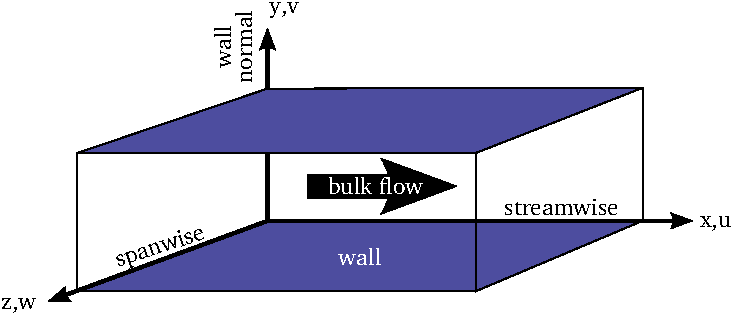
\includegraphics[width=0.495\textwidth]{ChannelSchematic}
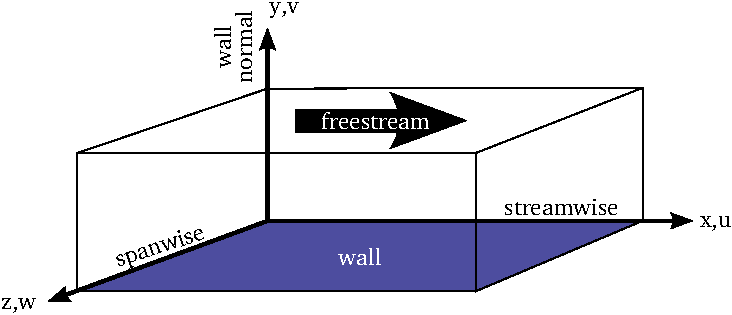
\includegraphics[width=0.495\textwidth]{FlatPlateSchematic}
\\
\caption[The channel and flat plate geometries]{%
  The channel (left) and flat plate (right) geometries. \label{fig:geometry}
}
\end{figure}

A mixed Fourier--Galerkin/B-spline collocation spatial
discretization is combined with a low-storage, semi-implicit third-order
Runge--Kutta scheme.  The spatial discretization yields excellent spectral
resolution~\citep{Kwok2001}, has long been proven for supersonic,
spatially homogenized boundary layer simulations~\citep{Guarini2000Direct}, and
provides a natural, scalable parallel domain decomposition on high-performance computing
environments.  The temporal discretization, used repeatedly at large
scale~\citep[e.g.][]{Hoyas2006Scaling} since its
introduction~\citep{spalart_lowstoragerk}, mitigates the potentially severe
acoustic and diffusive stability limits present in our problems of interest.
Nondimensional density $\rho$, momentum $m=\rho{}u$, and total energy
$e=\rho{}E$ were used as state variables.

%While many of the choices documented below have practical ramifications for
%the proposed simulation campaign and represent a large part of the work
%completed to date, the numerics are not genuinely new.  Accordingly, \emph{the
%remainder of this subsection may be skipped without loss of continuity.}

\subsection{Fourier/B-Spline Spatial Discretization}
\label{sec:spatialdiscretization}

Mimicking the governing equations in \autoref{sec:goveqn}, consider the abstract
continuous system
\begin{align}
  \frac{\partial\!u}{\partial\!t} &= \mathscr{L}u + \mathscr{N}\!\left(u\right)
\end{align}
on the spatial domain $\left[-\frac{L_x}{2},\frac{L_x}{2}\right] \times{}
[0,L_y] \times{} \left[-\frac{L_z}{2},\frac{L_z}{2}\right]$.  The operators
$\mathscr{L}$ and $\mathscr{N}$ are linear and nonlinear, respectively.
%For
%brevity, this section suppresses any time dependence in the operators.
To discretize this system, introduce its finite dimensional analog
\begin{align}
  \frac{\partial\!u^h}{\partial\!t}
  &=
  \mathscr{L}u^h + \mathscr{N}\!\left(u^h\right) + R^h
  \label{eq:discrete_system_with_residual}
\end{align}
where the continuous field $u = u\!\left(x,y,z,t\right)$ has been replaced by the discrete
field $u^h = u^h\!\left(x,y,z,t\right)$ with $N_x\times{}N_y\times{}N_z$ degrees of
freedom, and $R^h$ is the discretization error.
Fourier expansions are selected for the periodic $x$ and $z$ directions while a
B-spline expansion is adopted for the aperiodic $y$ direction.  That is,
\begin{align}
u^h(x,y,z,t)
&=
  \sum_{l=0}^{N_y - 1}
  \sum_{m=-\frac{N_x}{2}}^{\frac{N_x}{2}-1}
  \sum_{n=-\frac{N_z}{2}}^{\frac{N_z}{2}-1}
  \hat{u}_{l m n}(t)
  B_l\!\left(y\right)
  e^{\ii\frac{2\pi{}m}{L_x}x}
  e^{\ii\frac{2\pi{}n}{L_z}z}
  \notag\\
&=
  \sum_{l}\sum_{m}\sum_{n}
  \hat{u}_{l m n}(t)B_l\!\left(y\right)e^{\ii k_m x}e^{\ii k_n z}
  \label{eq:u_h_expansion}
\end{align}
where $k_m = 2\pi{}m/L_x$, $k_n = 2\pi{}n/L_z$, and $B_l\!\left(y\right)$ are a
B-spline basis for some order and knot selection.

Applying the method of weighted residuals, a mixed Galerkin/collocation
approach (often called a ``pseudospectral'' technique) is chosen that employs
the $L_{2}$ inner product and test ``functions'' like $\delta(y-y_{l'}) e^{\ii
k_{m'} x}e^{\ii k_{n'} z}$ where $l'$, $m'$, and $n'$ range over the same
values as $l$, $m$, and $n$, respectively.  The fixed collocation points
$y_{l'}$ depend on the B-spline basis details.  Three orthogonality
results are
\begin{subequations}
\begin{align}
   \int_0^{L_y} \varphi(y) \, \delta(y-y_{l'}) \,d\!y
&= \varphi(y_{l'})
\\
   \int_{-\frac{L_x}{2}}^{\frac{L_x}{2}} e^{\ii k_m x} e^{-\ii k_{m'} x} \,d\!x
&= L_x \delta_{m m'}
\\
   \int_{-\frac{L_z}{2}}^{\frac{L_z}{2}} e^{\ii k_n z} e^{-\ii k_{n'} z} \,d\!z
&= L_z \delta_{n n'}
\end{align}
\end{subequations}
where the inner product's conjugate operation is accounted for by introducing a
negative sign into the latter two exponentials.  The weighted residual is
forced to be zero in the sense that
\begin{align}
  \int_0^{L_y}
  \int_{-\frac{L_x}{2}}^{\frac{L_x}{2}}
  \int_{-\frac{L_z}{2}}^{\frac{L_z}{2}}
  R^h\!\left(x,y,z\right) \delta(y-y_{l'}) e^{-\ii k_{m'} x}e^{-\ii k_{n'} z}
  \,d\!z \,d\!x \,d\!y
  &=
  0
  \label{eq:R_h_weighted_residual_zero}
\end{align}
holds for all $l'$, $m'$, and $n'$.  Inserting \eqref{eq:u_h_expansion} into
\eqref{eq:discrete_system_with_residual}, testing with the test functions,
applying \eqref{eq:R_h_weighted_residual_zero}, and simplifying
\begin{align}
  L_x L_z
  \sum_{l} &B_l\!\left(y_{l'}\right)
  \frac{\partial\!}{\partial\!t} \hat{u}_{l m n}(t)
\notag\\
  &=
  L_x L_z
  \mathscr{L}\left(
    \sum_{l}
     B_l\!\left(y_{l'}\right)
    \hat{u}_{l m n}(t)
  \right)
\notag\\
  &{}+
  \int_{-\frac{L_x}{2}}^{\frac{L_x}{2}}
  \int_{-\frac{L_z}{2}}^{\frac{L_z}{2}}
  \mathscr{N}\left(
    \sum_{m}\sum_{n}
    \left(
      \sum_{l} B_l\!\left(y_{l'}\right)
      \hat{u}_{l m n}(t)
    \right)
    e^{\ii k_m x}e^{\ii k_n z}
  \right)
  \left(
    e^{-\ii k_{m'} x}e^{-\ii k_{n'} z}
  \right)
  \, dz \, dx.
\end{align}
Approximating the two integrals by discrete sums and dividing
by $L_x$ and $L_z$,
\begin{align}
  \sum_{l} &B_l\!\left(y_{l'}\right)
  \frac{\partial\!}{\partial\!t} \hat{u}_{l m n}(t)
\notag\\
  &\approx
  \mathscr{L}\left(
    \sum_{l}
     B_l\!\left(y_{l'}\right)
    \hat{u}_{l m n}(t)
  \right)
\notag\\
  &{}+
  \frac{1}{N_x N_z}
  \sum_{m'} \sum_{n'}
  \mathscr{N}\left(
    \sum_{m}
    \sum_{n}
    \left(
      \sum_{l} B_l\!\left(y_{l'}\right)
      \hat{u}_{l m n}(t)
    \right)
    e^{\ii k_m x_{m'}}e^{\ii k_n z_{n'}}
  \right)
  \!\!
  \left(
    e^{-\ii k_{m'} x_m}e^{-\ii k_{n'} z_n}
  \right)
  \label{eq:spatial_discretization}
\end{align}
where $x_{m'}=L_x m' / N_x$ and $z_{n'}=L_z n' / N_z$.
%
%%This approximation is
%%nothing but a quadrature error \citep[see][theorem~19]{Boyd2001}.  With
%%knowledge of the nonlinear operator $\mathscr{N}$, such quadrature error can be
%%mitigated via an appropriate dealiasing technique~\citep{Canuto2006}.
%%Three-halves dealiasing is selected.
The quadrature error in this approximation can be controlled by increasing the
number of quadrature points~\citep{Boyd2001}.  Here $3 N_x/2$ and $3 N_z/2$
quadrature points were used in $x$ and $z$, which eliminates quadrature error
when $\mathscr{N}$ is quadratic~\citep{Canuto2006}.  This approach has been
found to reduce quadrature error to acceptable levels for the compressible
Navier--Stokes equations~\citep{Buell1990Direct}.

Result~\eqref{eq:spatial_discretization} represents $N_x\times{}N_z$
time-dependent systems containing $N_y$ equations coupled in the $x$ and $z$
directions only through discrete Fourier transforms and the requirements of the
$\mathscr{L}$ and $\mathscr{N}$ operators.  Its left hand side has a
time-independent mass matrix arising from the B-spline basis and collocation
point choices.  The mass matrix is retained on the same side as the time
derivative in anticipation of the time discretization scheme.  The constant
factor $\left(N_x N_z\right)^{-1}$ also will be accommodated during time
advance.

\subsection{Semi-Implicit, Low-Storage Temporal Discretization}
\label{sec:timediscretization}

Time is advanced via the low-storage, semi-implicit scheme from
\citet*[Appendix A]{spalart_lowstoragerk} extended following
\citet{ShanYang2011}.  The ``SMR91'' scheme advances the system
\begin{align}
\label{eq:timediscretization}
 M u_t &= Lu + \chi{} N(u,t)
\end{align}
from $u\left(t\right)$ to $u\left( t+\Delta{}t \right)$.  Here $L$ and $N$ are a linear
and nonlinear operator, respectively, distinct from but related to the
preceding section's $\mathscr{L}$ and $\mathscr{N}$.  Both operators take the state
to an isomorphic, non-state representation from which the state can be recovered by
the action of the linear ``mass matrix'' $M$.
%
The constant $\chi$ permits scaling $\mathscr{N}$ during time advance; it will later
be used to apply the factor $\left(N_x N_z\right)^{-1}$ from
\eqref{eq:spatial_discretization}.
%
The scheme treats
$\chi{}M^{-1}N$ with third-order accuracy and $M^{-1}L$ with second-order
accuracy.

Each substep $i\in\left\{ 1,2,3 \right\}$ possesses the form
\begin{align}
  \left(M - \Delta{}t\beta_{i}{L}\right) u^{i+1}
  &=
  \left(M + \Delta{}t\alpha_{i}{L}\right) u^{i}
\notag\\
 &+ \Delta{}t\gamma_{i}\chi{}
    {N}\left(u^{i}, t_{n}+\eta_{i}\Delta{}t\right)
\notag\\
 &+ \Delta{}t\zeta_{i-1}\chi{}
    {N}\left(u^{i-1}, t_{n}+\eta_{i-1}\Delta{}t\right)
  \label{eq:generaloperatormasssubstep}
\end{align}
and uses the following substep-specific coefficients:
\begin{align*}
  \alpha_1, \alpha_2, \alpha_3 &= \left\{
    \frac{29}{96}, -\frac{3}{40},  \frac{1}{6}
  \right\}
  &
  \beta_1, \beta_2, \beta_3 &= \left\{
    \frac{37}{160}, \frac{5}{24}, \frac{1}{6}
  \right\}
  &
  \gamma_1, \gamma_2, \gamma_3 &= \left\{
    \frac{8}{15}, \frac{5}{12}, \frac{3}{4}
  \right\}
\end{align*}
\begin{align*}
  \zeta_0, \zeta_1, \zeta_2 &= \left\{
    0, -\frac{17}{60}, -\frac{5}{12}
  \right\}
  &
  \eta_0, \eta_1, \eta_2, \eta_3 &= \Biggl\{
    0, 0, \frac{8}{15}, \frac{2}{3}
  \Biggr\}.
\end{align*}
As shown, $L$ is time-independent throughout each interval $\left[t,
t+\Delta{}t\right)$ but $N$~is permitted to vary in time.

The scheme~\eqref{eq:generaloperatormasssubstep} requires implementations
of $u\mapsto{}{N}\left(u\right)$, $u\mapsto{}\left(M+\varphi{}L\right)u$, and
$u\mapsto{}\left(M+\varphi{}L\right)^{-1}u$ for a given $M$ and some arbitrary
scalar $\varphi$.  To require only two storage locations $a$ and $b$, the
$N\left(u\right)$ and $\left(M+\varphi{}L\right)^{-1}$ implementations must
operate in-place while $\left(M+\varphi{}L\right)$ must operate out-of-place.
Two issues bear attention.  First, the step size $\Delta{}t$ needs to be
dynamically computable based on a stability criterion accessible only during
the first nonlinear operator application.  Second, memory usage can be reduced
by applying $N$ against only one storage location, say $b$, so that only one
location requires auxiliary padding for quadrature.  Taken together,
$\left(M+\varphi{}L\right)$ also must support in-place application and
therefore storage
$a$ and $b$ should support a swap operation, $a\leftrightarrow{}b$.

\begin{algorithm}
\caption{Perform the three-step, low-storage time advance
         described in \textsection\ref{sec:timediscretization}}
\label{alg:step}
\begin{algorithmic}
  \renewcommand{\algorithmiccomment}[1]{\hfill{}// #1}
  \REQUIRE Storage $a = u\left(t_{n}\right) = u^{0} $;
           storage $b$ content undefined
  \STATE $b\leftarrow{}a$
  \STATE $b\leftarrow{}N\left(b,t_{n}\right)$
  \STATE Compute $\Delta{}t$ from $a=u^0$ and $b=N\left(u^0,t_{n}\right)$
  \STATE $a\leftarrow{}\left(M+\Delta{}t\alpha_{1}L\right)a$
  \STATE $a\leftarrow{}\Delta{}t \gamma_{1} \chi{} b + a$
  \STATE $a\leftarrow{}\left(M-\Delta{}t\beta_{1}L\right)^{-1}a$
  \ENSURE Storage $a = u^1$;
          storage $b = N\left(u^{0},t_{n}\right)$
  \STATE $b\leftarrow{}   \left(M+\Delta{}t\alpha_{2}L\right)a
                        + \Delta{}t\zeta_{1}\chi{}b$
  \STATE $a\leftrightarrow{}b$
  \STATE $b\leftarrow{}N\left(b,t_{n}+\eta_{2}\Delta{}t\right)$
  \STATE $a\leftarrow{}\Delta{}t \gamma_{2} \chi{} b + a$
  \STATE $a\leftarrow{}\left(M-\Delta{}t\beta_{2}L\right)^{-1}a$
  \ENSURE Storage $a = u^{2}$;
          storage $b = N\left(u^{1},t_{n}+\eta_{2}\Delta{}t\right)$
  \STATE $b\leftarrow{}   \left(M+\Delta{}t\alpha_{3}L\right)a
                        + \Delta{}t\zeta_{2}\chi{}b$
  \STATE $a\leftrightarrow{}b$
  \STATE $b\leftarrow{}N\left(b,t_{n}+\eta_{3}\Delta{}t\right)$
  \STATE $a\leftarrow{}\Delta{}t \gamma_{3} \chi{}b + a$
  \STATE $a\leftarrow{}\left(M-\Delta{}t\beta_{3}L\right)^{-1}a$
  \ENSURE Storage $a = u\left(t+\Delta{}t\right)= u^{3}$;
          storage $b = N\left(u^{2},t_{n}+\eta_{3}\Delta{}t\right)$
\end{algorithmic}
\end{algorithm}

In conclusion, time is advanced by one full step per Algorithm~\ref{alg:step}.
Using~\eqref{eq:generaloperatormasssubstep} to advance state $\hat{u}_{l m
n}(t)$ per~\eqref{eq:spatial_discretization} finally unites the spatial and
temporal operator notion used in this and the preceding subsection:
\begin{subequations}
\label{eq:uniteddiscretization}
\begin{align}
   M u\bigr|_{m n}
&= \sum_{l} B_l\!\left(y_{l'}\right)
   \hat{u}_{l m n}
\\
   \left.{L} u\right|_{m n}
&= \mathscr{L}\left(
     \sum_{l}
     B_l\!\left(y_{l'}\right)
     \hat{u}_{l m n}
   \right)
\\
   \left.{N}\!\left(u\right)\right|_{m n}
&= \underbrace{\frac{1}{N_x N_z}}_{\chi}
   \sum_{m'} \sum_{n'}
   \mathscr{N}\left(
     \sum_{m}
     \sum_{n}
     \left(
       \sum_{l} B_l\!\left(y_{l'}\right)
       \hat{u}_{l m n}
     \right)
     e^{\ii k_m x_{m'}}e^{\ii k_n z_{n'}}
   \right)
   \left(
     e^{-\ii k_{m'} x_m}e^{-\ii k_{n'} z_n}
   \right).
\end{align}
\end{subequations}

Time advancement occurs in ``coefficient'' or ``wave'' space but nonlinear terms
must be computed at ``collocation points'' or in ``physical'' space.  The parallel
communication and on-node computation cost required to convert state data from
wave space to physical space or vice versa can be high.  Consequently, many of
the following numerical choices were made to maximize both the amount of
simulation time advanced per Runge--Kutta step and to maintain as much numerical
resolution as possible.

\subsection{Discrete B-Spline Operators}
\label{sec:bsplineoperators}

Discrete operators for differentiation in the wall-normal direction map
B-spline coefficients to derivatives at wall-normal collocation points.  That
is,
\begin{align}
  D^{(j)} u\bigr|_{m n}
&= \sum_{l} B^{(j)}_l\!\left(y_{l'}\right)
   \hat{u}_{l m n}
\end{align}
where the banded matrix $D^{(j)}$ is wavenumber independent.  $D^{(0)}$ is
the ``mass matrix''
\begin{align}
  M &= D^{(0)}.
\end{align}
Similar to, but different from, the approaches discussed by
\citet[\textsection{}2.1.3]{Kwok2001}, the present work uses the Greville
abscissae, also called the Marsden--Schoenberg points, as its collocation points
\citep{Johnson2005Higher,Botella2003Bspline}.  Selecting these abscissae
automatically avoids the near-wall stability problems empirically circumvented
by \citet[\textsection{}4.4]{Kwok2001}.  Boundary treatments for B-spline
collocation operators use the property that the $j^\mathrm{th}$ derivative of the function
at the first (last) collocation point depends only on the first (last) $j+1$
B-spline coefficients.

For some uniform B-spline order $k$ and wall-normal number of degrees of
freedom $N_y$, $N_y - k + 2$ breakpoint locations must be specified.  Here
$k=4$ denotes a piecewise cubic basis.  For the channel geometry,
a two-sided hyperbolic tangent function~\citep{Vinokur1983Onedimensional}
stretches these breakpoints via
$f_2:\left[0,1\right]\to\left[0,1\right]$:
\begin{align}\label{eq:htstretch2}
  f_2\!\left(y\right) &= \frac{1}{2}\left(1 + \frac{%
      \tanh\left(\left(y-1/2\right)\delta\right)
  }{%
      \tanh\left(\delta/2\right)
  }\right).
\end{align}
For the flat plate, a one-sided hyperbolic tangent stretching
function~\citep{Vinokur1983Onedimensional} is applied per
$f_1:\left[0,1\right]\to\left[0,1\right]$:
\begin{align}\label{eq:htstretch1}
  f_1\!\left(y\right) &= 1 + \frac{%
      \tanh\left(\left(y-1\right)\delta\right)
  }{%
      \tanh\left(\delta\right)
  }.
\end{align}
Here $\delta\geq{}0$ is an adjustable stretching parameter where setting
$\delta=0$ recovers uniform spacing.  Values like $1\leq{}\delta\leq{}3$ are
used in practice.  After mapping uniform points on $\left[0,1\right]$ to
stretched points on $\left[0,1\right]$ using $f_2$ or $f_1$, a further affine
transformation is then used to map the breakpoints onto $\left[0, L_y\right]$.
These breakpoint locations on $\left[0, L_y\right]$ fix the collocation points
and consequently the collocation-based discrete operators $D^{(j)}$ through the
definition of the Greville abscissae applied for order $k$.

Unlike Fourier-based derivatives, with B-splines applying $D^{(1)}D^{(1)}$ gives
a result that differs significantly from applying $D^{(2)}$ because repeated first
differentiation severely abates high frequency
modes~\citep[Figures~2--3]{Kwok2001}.  Second derivatives enter
\eqref{eq:nondim_model} only through terms $\nabla\cdot\tau$, $\nabla\cdot\tau{}u$,
and $\nabla\cdot\mu\nabla{}T$.  These first and second derivative applications
are computed wholly separately to discretely obtain the most physically consistent
dissipation of high-frequency content at a given spatial resolution.  This
decision comes with additional implementation complexity, see
\autoref{tab:nofirstderivnonlinearcost}, but this choice
eliminated any need to add aphysical discrete filtering which is often used to
prevent the catastrophic buildup of spurious numerical noise.

%%%%%%%%%%%%%%%%%%%%%%%%%%%%%%%%%%%%%%%%%%%%%%%%%%%%%%%%%%%%%%%%%%%%%%%%%%%%%%
%%%%%%%%%%%%%%%%%%%%%%%%%%%%%%%%%%%%%%%%%%%%%%%%%%%%%%%%%%%%%%%%%%%%%%%%%%%%%%
\begin{table}[p]{% Extra braces for temporary scope
\centering
\caption[%
    Communications overhead inherent to computing quantities without repeated
    first differentiation.
]{%
    Communications overhead inherent to computing quantities without repeated
    first differentiation.  Overhead measured relative to transforming a single
    scalar field from wave space to physical space.  A check (\checkmark)
    indicates that a quantity is required to compute terms in the leftmost
    column.  A bullet ($\bullet$) indicates the quantity is required but it can
    be computed from other required quantities.  Total costs for each term are
    summarized in the rightmost column.
}
\label{tab:nofirstderivnonlinearcost}
\renewcommand{\arraystretch}{1.30}      % Adds whitespace between rows
\makecommand{\cm}{\checkmark}           % For brevity in the table details
\makecommand{\cd}{\ensuremath{\bullet}} % For brevity in the table details
\vspace{1em}
\makebox[\textwidth][c]{\resizebox{6.4in}{!}{%
\begin{tabular}{r|cccc|cccccc|ccc|r}
% 001 & 002 & 003 & 004 & 005 & 006 & 007 & 008 & 009 & 011 & 012 & 013 & 014
&   1 &   3 &   1 &   6 &   3 &   1 &   6 &   9 &   3 &   3 &   1 &   3 &   1
\\
& $\rho$                                              % 01
& $\nabla\rho$                                        % 02
& $\Delta\rho$                                        % 03
& $\nabla\nabla\rho$                                  % 04
& $m$                                                 % 05
& $\nabla\cdot{}m$                                    % 06
& $\symmetricpart{\nabla{}m}$                         % 07
& $\nabla{}m$                                         % 08
& $\Delta{}m$                                         % 09
& $\nabla\nabla\cdot{}m$                              % 11
& $e$                                                 % 12
& $\nabla{}e$                                         % 13
& $\Delta{}e$                                         % 14
\\ \hline
$\nabla\cdot\frac{m}{\rho}$
% 001 & 002 & 003 & 004 & 005 & 006 & 007 & 008 & 009 & 011 & 012 & 013 & 014
& \cm & \cm &     &     & \cm & \cm &     &     &     &     &     &     &
& 8 \\
$\nabla\frac{m}{\rho}$
% 001 & 002 & 003 & 004 & 005 & 006 & 007 & 008 & 009 & 011 & 012 & 013 & 014
& \cm & \cm &     &     & \cm &     &     & \cm &     &     &     &     &
& 16 \\
$\symmetricpart{\nabla\frac{m}{\rho}}$
% 001 & 002 & 003 & 004 & 005 & 006 & 007 & 008 & 009 & 011 & 012 & 013 & 014
& \cm & \cm &     &     & \cm &     & \cm &     &     &     &     &     &
& 13 \\
$\Delta\frac{m}{\rho}$
% 001 & 002 & 003 & 004 & 005 & 006 & 007 & 008 & 009 & 011 & 012 & 013 & 014
& \cm & \cm & \cm &     & \cm &     &     & \cm & \cm &     &     &     &
& 20 \\
$\nabla\nabla\cdot\frac{m}{\rho}$
% 001 & 002 & 003 & 004 & 005 & 006 & 007 & 008 & 009 & 011 & 012 & 013 & 014
& \cm & \cm &     & \cm & \cm & \cd &     & \cm &     & \cm &     &     &
& 25 \\[1.5em]
$p$, $T$, $\mu$, $\lambda$
% 001 & 002 & 003 & 004 & 005 & 006 & 007 & 008 & 009 & 011 & 012 & 013 & 014
& \cm &     &     &     & \cm &     &     &     &     &     & \cm &     &
& 5 \\
$\nabla{}p$, $\nabla{}T$, $\nabla\mu$, $\nabla\lambda$
% 001 & 002 & 003 & 004 & 005 & 006 & 007 & 008 & 009 & 011 & 012 & 013 & 014
& \cm & \cm &     &     & \cm &     &     & \cm &     &     & \cm & \cm &
& 20 \\
$\Delta{}p$
% 001 & 002 & 003 & 004 & 005 & 006 & 007 & 008 & 009 & 011 & 012 & 013 & 014
& \cm & \cm & \cm &     & \cm &     &     & \cm & \cm &     &     &     & \cm
& 21 \\
$\Delta{}T$
% 001 & 002 & 003 & 004 & 005 & 006 & 007 & 008 & 009 & 011 & 012 & 013 & 014
& \cm & \cm & \cm &     & \cm &     &     & \cm & \cm &     & \cm & \cm & \cm
& 25 \\[1.5em]
$\tau$
% 001 & 002 & 003 & 004 & 005 & 006 & 007 & 008 & 009 & 011 & 012 & 013 & 014
& \cm & \cm &     &     & \cm & \cd & \cm &     &     &     & \cm &     &
& 14 \\[1.5em]
$\symmetricpart{\nabla\frac{m}{\rho}} \nabla\mu$
% 001 & 002 & 003 & 004 & 005 & 006 & 007 & 008 & 009 & 011 & 012 & 013 & 014
& \cm & \cm &     &     & \cm &     & \cd & \cm &     &     & \cm & \cm &
& 20 \\
$\mu\Delta\frac{m}{\rho}$
% 001 & 002 & 003 & 004 & 005 & 006 & 007 & 008 & 009 & 011 & 012 & 013 & 014
& \cm & \cm & \cm &     & \cm &     &     & \cm & \cm &     & \cm &     &
& 21 \\
$\left(\mu+\lambda\right)\nabla\nabla\cdot\frac{m}{\rho}$
% 001 & 002 & 003 & 004 & 005 & 006 & 007 & 008 & 009 & 011 & 012 & 013 & 014
& \cm & \cm &     & \cm & \cm & \cd &     & \cm &     & \cm & \cm &     &
& 26 \\
$\left(\nabla\cdot\frac{m}{\rho}\right)\nabla\lambda$
% 001 & 002 & 003 & 004 & 005 & 006 & 007 & 008 & 009 & 011 & 012 & 013 & 014
& \cm & \cm &     &     & \cm & \cd &     & \cm &     &     & \cm & \cm &
& 20 \\
$\nabla\cdot\tau$
% 001 & 002 & 003 & 004 & 005 & 006 & 007 & 008 & 009 & 011 & 012 & 013 & 014
& \cm & \cm & \cd & \cm & \cm & \cd & \cd & \cm & \cm & \cm & \cm & \cm &
& 32 \\[1.5em]
$\frac{m}{\rho}\cdot\left(\nabla\cdot\tau\right)$
% 001 & 002 & 003 & 004 & 005 & 006 & 007 & 008 & 009 & 011 & 012 & 013 & 014
& \cm & \cm & \cd & \cm & \cm & \cd & \cd & \cm & \cm & \cm & \cm & \cm &
& 32 \\
$\trace\left(\trans{\tau}\nabla\frac{m}{\rho}\right)$
% 001 & 002 & 003 & 004 & 005 & 006 & 007 & 008 & 009 & 011 & 012 & 013 & 014
& \cm & \cm &     &     & \cm & \cd & \cd & \cm &     &     & \cm &     &
& 20 \\
$\nabla\cdot\tau\frac{m}{\rho}$
% 001 & 002 & 003 & 004 & 005 & 006 & 007 & 008 & 009 & 011 & 012 & 013 & 014
& \cm & \cm & \cd & \cm & \cm & \cd & \cd & \cm & \cm & \cm & \cm & \cm &
& 32 \\[1.5em]
$\nabla\mu\cdot\nabla{}T$
% 001 & 002 & 003 & 004 & 005 & 006 & 007 & 008 & 009 & 011 & 012 & 013 & 014
& \cm & \cm &     &     & \cm &     &     & \cm &     &     & \cm & \cm &
& 20 \\
$\mu\Delta{}T$
% 001 & 002 & 003 & 004 & 005 & 006 & 007 & 008 & 009 & 011 & 012 & 013 & 014
& \cm & \cm & \cm &     & \cm &     &     & \cm & \cm &     & \cm & \cm & \cm
& 25 \\
$\nabla\cdot\mu\nabla{}T$
% 001 & 002 & 003 & 004 & 005 & 006 & 007 & 008 & 009 & 011 & 012 & 013 & 014
& \cm & \cm & \cm &     & \cm &     &     & \cm & \cm &     & \cm & \cm & \cm
& 25
\end{tabular}
}}%resizebox
}\end{table}
%%%%%%%%%%%%%%%%%%%%%%%%%%%%%%%%%%%%%%%%%%%%%%%%%%%%%%%%%%%%%%%%%%%%%%%%%%%%%%
%%%%%%%%%%%%%%%%%%%%%%%%%%%%%%%%%%%%%%%%%%%%%%%%%%%%%%%%%%%%%%%%%%%%%%%%%%%%%%

\subsection{Time Step Stability Criteria}
\label{sec:stabilitycriteria}

The step size $\Delta{}t$ used in the SMR91 scheme is limited by both a
convective and a diffusive stability criterion.  The time step is taken to
be the largest stable time step possible according to both restrictions.  As
both criteria are approximate, the resulting $\Delta{}t$ is further multiplied
by a safety factor less than one.  Safety factors 0.70--0.77 are often
used~\citep{Venugopal2003,spalart_lowstoragerk}.  Efforts to improve stability
estimates for a given discretization are worthwhile because even small increases
in time step size can translate into appreciable compute savings over the course
of a long simulation.

\subsubsection{Convective Stability Limit from Scalar Analysis}
\label{sec:convectivestability}

The convective criterion uses the maximum imaginary eigenvalue magnitude from
the Euler equations as a surrogate for the more complicated Navier--Stokes
system.  Both \citet[Equation~2.39]{Kwok2002} and
\citet[Equations~4.20--21]{Guarini1998} derived the stability result
\begin{align}\label{eq:convectivestability}
  \Delta{}t &\leq
  \frac{%
    \left|\lambda_{I}\Delta{}t\right|_{\max}
  }{%
      \left(\left|u_{x}\right| + a\right) \lambda^{(1)}_x
    + \left(\left|u_{y}\right| + a\right) \lambda^{(1)}_y
    + \left(\left|u_{z}\right| + a\right) \lambda^{(1)}_z
  }
\end{align}
where $a$ is the local acoustic velocity, $u_{x}$ denotes the velocity in the
$x$ direction, $\lambda^{(1)}_x$ represents the maximum imaginary eigenvalue
magnitude of the first derivative operator in the $x$ direction, etc.  In the
two Fourier directions these eigenvalues are exactly known:
\begin{align}
    \lambda^{(1)}_x &= \frac{\pi N_x}{L_x} = \frac{\pi}{\Delta{}x},
    &
    \lambda^{(1)}_z &= \frac{\pi N_z}{L_z} = \frac{\pi}{\Delta{}z}.
\end{align}
For the B-spline operator $M^{-1} D^{(1)}$ which maps function coefficients to
first derivative coefficients, one may similarly estimate
\begin{align}\label{eq:lambda1deltay}
    \lambda^{(1)}_y &= \frac{\pi}{C^{(1)}\Delta{}y}
\end{align}
where the definition of $\Delta{}y$ and $C^{(1)}$ are for now deferred.
Analogously to the Fourier case, for a periodic, uniform B-spline basis,
$C^{(1)}$ would be one.  The maximum pure imaginary eigenvalue magnitude,
$\left|\lambda_{I}\Delta{}t\right|_{\max}$, is a feature of the chosen
time-stepping method.  For the SMR91 scheme,
\begin{align}
  \left|\lambda_{I}\Delta{}t\right|_{\max} &= \sqrt{3}.
\end{align}

For nondimensional formulations in which an explicit Mach number,
$\mbox{Ma}=u_0/a_0$ appears, one must provide the velocities and the
sound speed both nondimensionalized using $u_0$.  Expressions like
$\left|u\right| + a/\mbox{Ma}$ are appropriate for this context, as can be
seen by finding the eigenvalues of the Euler equations in such a
nondimensionalization.  Using an A-stable scheme, like the implicit portion of
SMR91, to compute acoustic terms effectively sets the sound speed to zero when
computing this convective criterion.

Returning to Equation~\eqref{eq:lambda1deltay}, both
\citeauthor{Guarini1998} and \citeauthor{Kwok2002} used the breakpoint
separation for $\Delta{}y$ and set $C^{(1)} = 1$.  When
\citeauthor{Venugopal2003} used a nearly identical convective criterion
to~\eqref{eq:convectivestability}, he found using $C^{(1)} = 1$ to be overly
conservative for aperiodic $D^{(1)}$ built from nonuniform breakpoints.
\citet[\textsection{}3.2]{Venugopal2003} presented a linearized analysis taking
into account the inhomogeneous nature of his wall-normal direction.  He
determined that the wall-normal imaginary eigenvalue magnitude dropped by nearly
an order of magnitude after taking into account the inhomogeneity.  He concluded
that, taking $\Delta{}y$ to be the breakpoint separation, $C^{(1)} = 4$ was
feasible \citep[Equation~3.29]{Venugopal2003}.  The present choice of
$\Delta{}y$ and $C^{(1)}$ is discussed after the diffusive stability limit.

\subsubsection{Diffusive Stability Limit from Scalar Analysis}
\label{sec:diffusivestability}

The diffusive criterion uses the maximum real eigenvalue magnitude from a model
diffusion equation as a surrogate for the more complicated Navier--Stokes
system.
Both \citet[Equation~2.40]{Kwok2002} and
\citet[Equations~4.29--30]{Guarini1998} derived the stability
result
\begin{align}\label{eq:diffusivestability}
    \Delta{}t &\leq
    \frac{%
        \left|\lambda_{R}\Delta_{}t\right|_{\max}
    }{%
      \max\left(
        \left|\frac{\gamma\left(\nu-\nu_{0}\right)}{\mbox{Re}\mbox{Pr}}\right|,
        \left|\frac{\nu-\nu_{0}}{\mbox{Re}}\right|,
        \left|\frac{\nu_{B}-\nu_{B0}}{\mbox{Re}}\right|
      \right)
      \left(
          \lambda^{(2)}_x
        + \lambda^{(2)}_y
        + \lambda^{(2)}_z
      \right)
    }
\end{align}
where a bulk kinematic viscosity has been added to their results.  As in the
convective criterion, in the Fourier direction these eigenvalues are exactly
known and we introduce $C^{(2)}$ in the wall-normal B-spline direction:
\begin{align}\label{eq:lambda2deltay}
    \lambda^{(2)}_x &= \left(\frac{\pi N_x}{L_x}\right)^2
                     = \frac{\pi^2}{\Delta{}x^2},
    &
    \lambda^{(2)}_y &= \left(\frac{\pi}{C^{(2)} \Delta{}y}\right)^2,
    &
    \lambda^{(2)}_z &= \left(\frac{\pi N_z}{L_z}\right)^2
                     = \frac{\pi^2}{\Delta{}z^2}.
\end{align}
Here $M^{-1}D^{(2)}$ is the B-spline operator of interest, which maps function
coefficients to second derivative coefficients.  Again, the definition of
$\Delta{}y$ and $C^{(2)}$ are for now deferred.  The maximum pure real
eigenvalue magnitude, $\left|\lambda_{R}\Delta{}t\right|_{\max}$, is a feature
of the chosen time-stepping method.  For the SMR91 scheme,
\begin{align}
\left|\lambda_{R}\Delta{}t\right|_{\max} &\approx 2.512.
\end{align}
Using an A-stable scheme, like the implicit portion of SMR91, to compute
linearized viscous terms allows subtracting the linearization reference
kinematic viscosities $\nu_0$ and $\nu_{B0}$ when computing this diffusive
criterion.  The absolute values within the maximum operations account for the
possibility that $\nu<\nu_{0}$.

Returning to Equation~\eqref{eq:lambda2deltay}, both
\citeauthor{Guarini1998} and \citeauthor{Kwok2002} used the breakpoint
separation for $\Delta{}y$ and set $C^{(2)} = 1$.  \citeauthor{Venugopal2003}
used a nearly identical diffusive criterion
\citep[Equation~3.15]{Venugopal2003}.  His analysis determined that the
diffusive stability criterion was not overly conservative for an aperiodic
B-spline discretization.  The present choices for $\Delta{}y$ and $C^{(2)}$
are discussed next.

\subsubsection{Empirical Limits for Inhomogeneous B-Spline Operators}
\label{sec:wallnormaleigval}

Employing stability estimates \eqref{eq:convectivestability}
and~\eqref{eq:diffusivestability} requires information about the wall-normal
discrete operator eigenvalue magnitudes.  By Equations~\eqref{eq:lambda1deltay}
and~\eqref{eq:lambda2deltay} this is equivalent to estimating both $C^{(1)}$
and $C^{(2)}$.  Per \autoref{sec:bsplineoperators}, our operators are a
function of three parameters: the piecewise polynomial order $k$ where $k=4$
indicates piecewise cubic B-splines, the hyperbolic tangent stretching
parameter $\delta\geq{}0$, and the wall-normal number of degrees of freedom
$N_y\geq{}k$.

\begin{figure}
  \centering
  \vspace{-1em}
  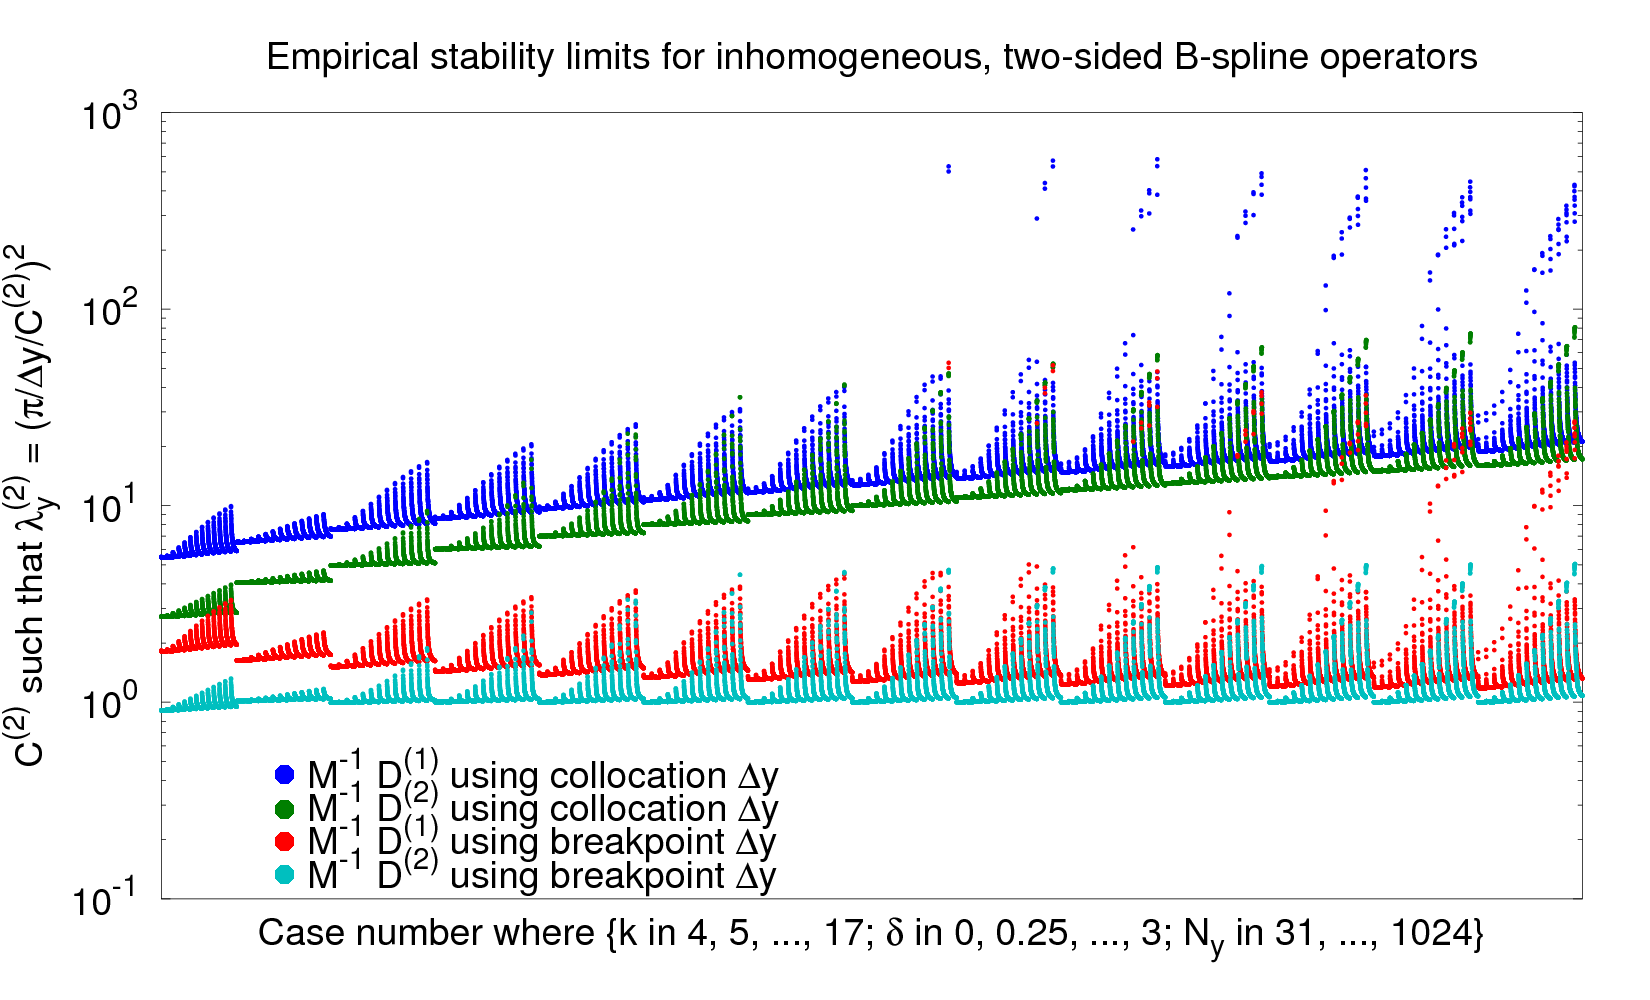
\includegraphics[width=5.5in]{inhomogeneity2}
  \\
  \vspace{0.5em}
  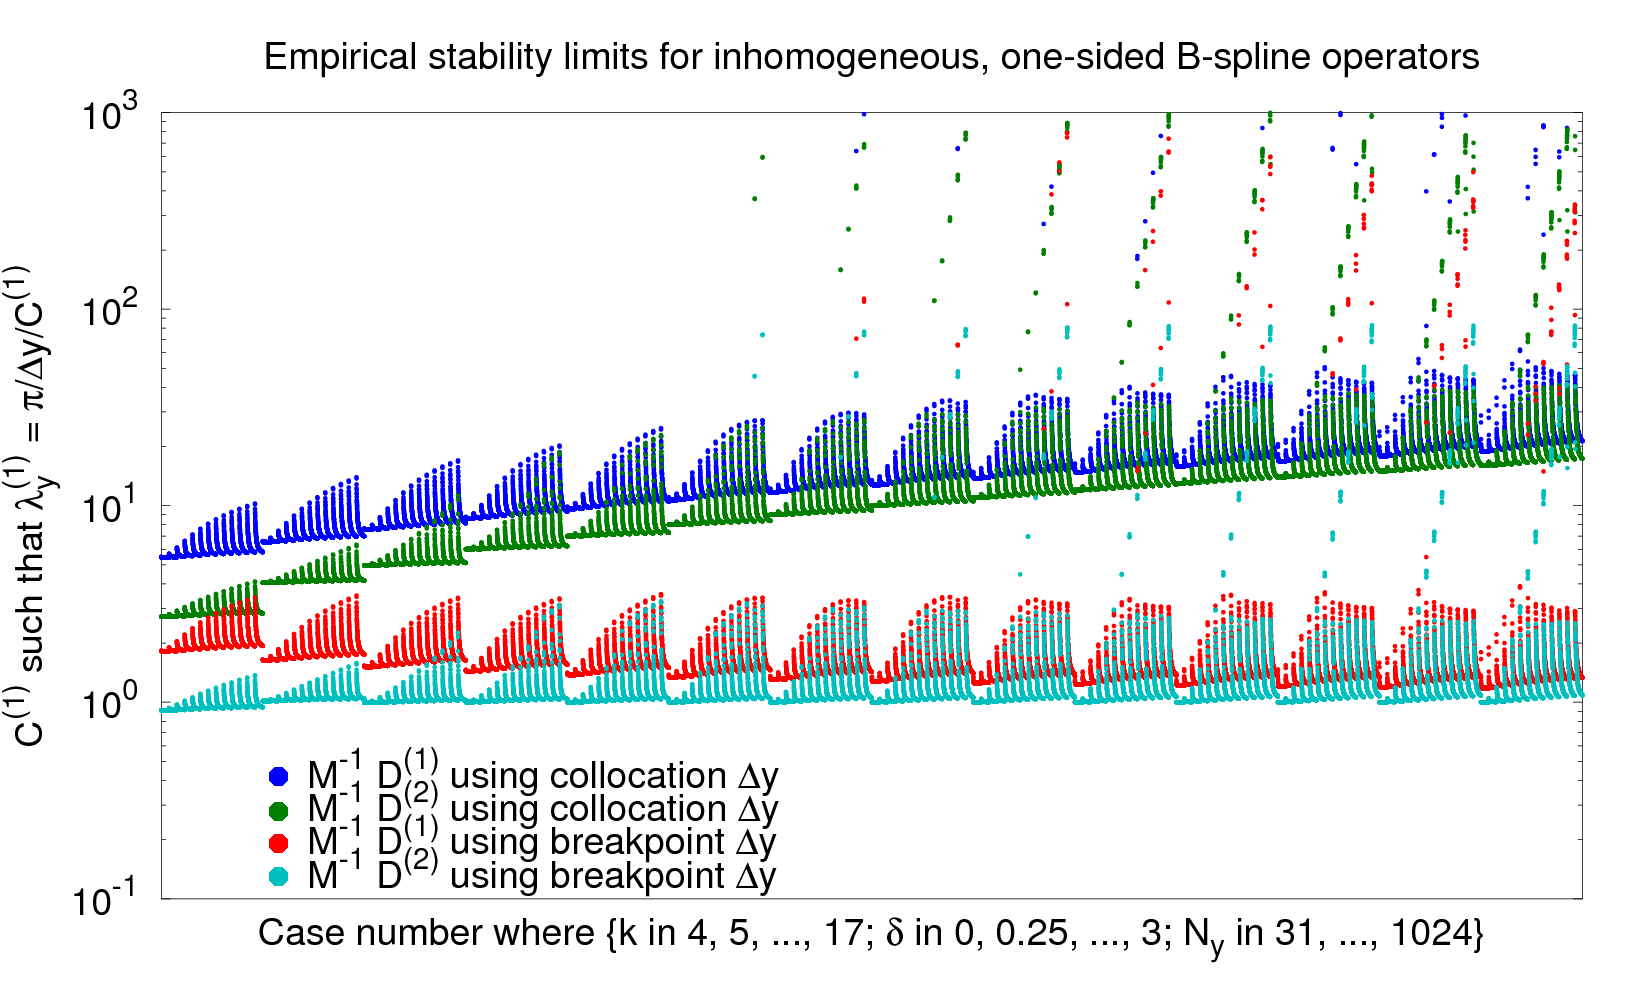
\includegraphics[width=5.5in]{inhomogeneity1}
  \\
  \caption[Exact maximum eigenvalues for inhomogeneous B-spline operators]{%
  Exact values of $C^{(1)}$ and $C^{(2)}$ computed per
  Equations~\eqref{eq:lambda1deltay} and~\eqref{eq:lambda2deltay} for roughly
  32,500 combinations of $k$, $\delta$, and $N_y$.  Above, two-sided stretching
  was performed on breakpoints per~\eqref{eq:htstretch2}.  Below, one-sided
  stretching was performed per~\eqref{eq:htstretch1}.  In both figures, the
  leftmost four ``triangles'' correspond to $k=4$ while $\delta$ was varied
  slowly and $N_y$ varied quickly.  Moving rightward, the next ``triangles''
  are for $k=5$, then $k=6$, etc.
  \label{fig:inhomogeneity}
  }
\end{figure}

Using numerically obtained eigenvalue magnitudes
$\lambda^{(1)}=\lambda^{(1)}_y\!\left(k,\delta,N_y\right)$ and
$\lambda^{(2)}=\lambda^{(2)}_y\!\left(k,\delta,N_y\right)$ from a large
collection of discrete operators, exact $C^{(1)}$ and $C^{(2)}$ values were
computed.  The results are shown in \autoref{fig:inhomogeneity}.  The minimum
grid spacing $\Delta{}y$ was measured using either adjacent breakpoints or
adjacent collocation points to permit a comparison.  Considering only
breakpoint-based results for $k=8$, one can see how \citet{Venugopal2003}
probably chose $C^{(1)}=4$ and $C^{(2)}=1$ as discussed in
\autoref{sec:convectivestability} and \autoref{sec:diffusivestability}.
However, it is striking just how nonuniversal those choices are.
Evidently, neither a breakpoint-based nor a collocation point-based $\Delta{}y$
inherently captures the maximum eigenvalue magnitudes as $k$, $\delta$, and
$N_y$ vary--- some nonlinear combination of the complete set of grid parameters
is necessary.

Hereafter, unlike \citeauthor{Guarini1998}, \citeauthor{Kwok2002}, and
\citeauthor{Venugopal2003}, we take $\Delta{}y$ to be the spacing between
adjacent collocation points.  Performing Levenberg--Marquardt nonlinear
regression against the vast majority of the empirical data in
\autoref{fig:inhomogeneity} shows good agreement with curve fits like the
following
\begin{subequations}
\begin{align}
  \label{eq:Cfit}
  C_\text{approx}^{(i)}\!\left(k,\delta,N_y\right)
  &\approx
    a k
  + b \hat\delta
  + \frac{c}{\sqrt{k}}
  + k^{d + e \hat\delta} \left(
        1 + \left(\frac{f k}{N_y - k + 1}\right)^{g k + h \hat\delta}
    \right)
  ,
  \\
  \hat\delta &= \left(1+\delta\right)^i \tanh \delta.
\end{align}
\end{subequations}
The data from ``nearly spectral'' discrete operators, defined as when $N_y \leq
5 k$, proved difficult to fit and was omitted.  Such cases look like outliers
in \autoref{fig:inhomogeneity} and are not operationally important as
the present work does not use a spectral wall-normal basis.  When
using two-sided stretching per~\eqref{eq:htstretch2}, one collection of
constants $a$--$i$ permits fitting the retained $C^{(1)}$ observations for
$k=5$ through $11$ to within relative errors of [-2.55\%, 1.76\%].  Another
collection permits fitting retained $C^{(2)}$ observations to within [-11.3\%,
17.1\%].  While those results are encouraging for the generality of the chosen
functional forms, they are less than satisfactory for production use.  More
precise, $k$-specific, coefficients for two-sided stretching appear in
\autoref{tab:C1fit2} and \autoref{tab:C2fit2} while coefficients for one-sided
stretching appear in \autoref{tab:C1fit1} and \autoref{tab:C2fit1}.

Unfortunately, using either $C_\text{approx}^{(1)}$ or $C_\text{approx}^{(2)}$
directly proved to be overly aggressive as measured using a collection of
contrived test problems known \emph{a priori} to be either convectively or
diffusively limited.  Scaling these by a single safety factor was problematic as no
unique value allowed pushing up against both criteria simultaneously.  Against
the same test problems, however, using approximations like the square root of
$C_\text{approx}^{(i)}$ did permit using a uniform safety factor across a
variety of test conditions.

In summary, the present work takes nearly the square root of a conservative
estimate of $C_\text{approx}^{(i)}$.  That is,
\begin{align}
  C^{(1)} &= \left(
      \frac{C_\text{approx}^{(1)}}
           {1 - \text{(negative relative error percentage)}/100}
  \right)^{33/64}
\\
  C^{(2)} &= \left(
      \frac{C_\text{approx}^{(2)}}
           {1 - \text{(negative relative error percentage)}/100}
  \right)^{27/64}
\end{align}
where the fit-specific, negative-valued lower error bounds appear in the
rightmost column of the coefficient tables.  Adjusting to the empirical fits'
lower bounds gives slightly more conservative $\lambda_y^{(i)}$ estimates.  These
values of $C^{(i)}$ are plugged into Equations~\eqref{eq:lambda1deltay}
and~\eqref{eq:lambda2deltay} with those results feeding into
Equations~\eqref{eq:convectivestability} and~\eqref{eq:diffusivestability}.
These estimates were designed for use with safety factors like 0.72 whenever
$N_y > 5k$,  which will be revisited in
\autoref{sec:channel_runs}.

\begin{sidewaystable}
\centering
\caption[
    B-spline order-specific curve fits for $C_\text{approx}^{(1)}$
    for stretching~\eqref{eq:htstretch2}.
]{%
    B-spline order-specific curve fits for estimating $C_\text{approx}^{(1)}$
    via Equation~\eqref{eq:Cfit} when $\Delta{}y$ is the minimum distance
    between \emph{collocation points} from breakpoints stretched according
    to $f_2$ defined in~\eqref{eq:htstretch2}.
}
\label{tab:C1fit2}
\vspace{1em}
\renewcommand{\arraystretch}{1.40}   % Adds whitespace between rows
\begin{tabular}{r|ccccccccc|c@{ -- }c@{\%}}
 $k$ & $a$ & $b$ & $c$ & $d$ & $e$ & $f$ & $g$ & $h$ & $i$
     & \multicolumn{2}{c}{relative error}
\\ \hline
%%%%%%%%%%
% TWOSIDED
%%%%%%%%%%
5--11
&  $\frac{            5054}{            4549}$
& -$\frac{            3953}{           12175}$
&  $\frac{            4321}{            5893}$
& -$\frac{            5839}{            8805}$
&  $\frac{            3121}{            7385}$
&  $\frac{          235081}{            5659}$
&  $\frac{             399}{           13421}$
&  $\frac{            2795}{            8687}$
&  $\frac{            3548}{            7037}$
&  -2.55 &  1.76
\\
4
&  $\frac{            8753}{            6138}$
&  $\frac{             184}{            3513}$
& -$\frac{            3868}{            6327}$
& -$\frac{           22756}{            5215}$
&  $\frac{           19435}{           28258}$
&  $\frac{       152882005}{            9731}$
&  $\frac{            1605}{           12298}$
&  $\frac{             814}{            5783}$
&  $\frac{            7755}{           19621}$
&  -1.52 &  0.46
\\
5
& -$\frac{          182723}{            7970}$
&  $\frac{             121}{            6080}$
& -$\frac{         7061095}{           23119}$
&  $\frac{          115483}{           33477}$
&  $\frac{               1}{            5560}$
&  $\frac{             197}{            3683}$
&  $\frac{             761}{            2741}$
& -$\frac{            2307}{            6251}$
&  $\frac{            1845}{            5548}$
&  -1.12 &  0.53
\\
6
&  $\frac{            8193}{            7183}$
&  $\frac{              74}{            7487}$
&  $\frac{           10787}{            6960}$
& -$\frac{           12529}{            6209}$
&  $\frac{            3196}{            4771}$
&  $\frac{         4441318}{           12819}$
&  $\frac{             932}{           12135}$
&  $\frac{            3915}{           17923}$
&  $\frac{             870}{            2123}$
&  -1.39 &  1.14
\\
7
&  $\frac{            9063}{            5683}$
&  $\frac{             291}{            6739}$
& -$\frac{           26786}{            3839}$
& -$\frac{            2757}{            1352}$
&  $\frac{            2959}{            4613}$
&  $\frac{         2666741}{            4919}$
&  $\frac{             507}{            6947}$
&  $\frac{             498}{            2627}$
&  $\frac{            3572}{            8791}$
&  -1.50 &  1.12
\\
8
&  $\frac{           20956}{           18111}$
&  $\frac{              73}{            3043}$
&  $\frac{            3316}{            4207}$
& -$\frac{           17945}{           10877}$
&  $\frac{            6659}{           11166}$
&  $\frac{         2564433}{            9169}$
&  $\frac{             658}{           10813}$
&  $\frac{            2725}{           12594}$
&  $\frac{            1181}{            2847}$
&  -1.48 &  1.18
\\
9
&  $\frac{            4351}{            3996}$
&  $\frac{             204}{            4093}$
&  $\frac{           13726}{            5957}$
& -$\frac{           19388}{           12047}$
&  $\frac{           10397}{           18003}$
&  $\frac{         1200048}{            3823}$
&  $\frac{             246}{            4289}$
&  $\frac{            1395}{            6839}$
&  $\frac{            4244}{           10183}$
&  -1.54 &  1.09
\\
10
&  $\frac{            3174}{            3221}$
&  $\frac{             340}{            4047}$
&  $\frac{          435835}{           78898}$
& -$\frac{           24457}{           14830}$
&  $\frac{            3057}{            5416}$
&  $\frac{         5464428}{           12505}$
&  $\frac{             166}{            3013}$
&  $\frac{             679}{            3691}$
&  $\frac{            2669}{            6422}$
&  -1.59 &  1.11
\\
11
&  $\frac{            6141}{            6356}$
&  $\frac{             513}{            5051}$
&  $\frac{           35557}{            5371}$
& -$\frac{            5359}{            3384}$
&  $\frac{            6824}{           12279}$
&  $\frac{         3628675}{            8504}$
&  $\frac{            1012}{           19681}$
&  $\frac{             363}{            2008}$
&  $\frac{            1873}{            4520}$
&  -1.56 &  0.94
\\
12
&  $\frac{            9953}{            8604}$
&  $\frac{             521}{            4751}$
& -$\frac{            2623}{            3140}$
& -$\frac{           12011}{            8190}$
&  $\frac{            9067}{           16522}$
&  $\frac{         1947584}{            5723}$
&  $\frac{             141}{            2959}$
&  $\frac{            1231}{            6652}$
&  $\frac{            8479}{           20445}$
&  -1.58 &  1.12
\\
13
&  $\frac{            6428}{            6247}$
&  $\frac{              28}{             239}$
&  $\frac{           28437}{            6178}$
& -$\frac{           13912}{           10071}$
&  $\frac{            2717}{            5125}$
&  $\frac{         3512083}{           11082}$
&  $\frac{             542}{           12275}$
&  $\frac{             701}{            3776}$
&  $\frac{            7291}{           17441}$
&  -1.58 &  1.08
\\
14
&  $\frac{           18221}{           17050}$
&  $\frac{             573}{            3767}$
&  $\frac{           37351}{           13944}$
& -$\frac{           12384}{            8881}$
&  $\frac{            2238}{            4193}$
&  $\frac{         3701821}{           10597}$
&  $\frac{             231}{            5389}$
&  $\frac{            2953}{           16836}$
&  $\frac{            3950}{            9507}$
&  -1.59 &  1.10
\\
15
&  $\frac{            9251}{            9369}$
&  $\frac{            1001}{            5400}$
&  $\frac{         1033331}{          141480}$
& -$\frac{           13367}{            9358}$
&  $\frac{            7583}{           14554}$
&  $\frac{         2662722}{            5819}$
&  $\frac{             392}{            9519}$
&  $\frac{             555}{            3394}$
&  $\frac{            2181}{            5234}$
&  -1.56 &  1.01
\\
16
&  $\frac{            8003}{            8200}$
&  $\frac{            2503}{           12108}$
&  $\frac{          263686}{           31457}$
& -$\frac{            5713}{            4107}$
&  $\frac{            4803}{            9290}$
&  $\frac{         8189082}{           18419}$
&  $\frac{              93}{            2371}$
&  $\frac{            1663}{           10299}$
&  $\frac{            2945}{            7073}$
&  -1.56 &  1.08
\\
17
&  $\frac{           10594}{            8835}$
&  $\frac{            2615}{           11361}$
& -$\frac{           38602}{            5641}$
& -$\frac{            3464}{            2537}$
&  $\frac{            3372}{            6575}$
&  $\frac{         4481119}{           10024}$
&  $\frac{             355}{            9469}$
&  $\frac{             811}{            5107}$
&  $\frac{            1129}{            2714}$
&  -1.53 &  0.97
\end{tabular}
\end{sidewaystable}

\begin{sidewaystable}
\centering
\caption[
    B-spline order-specific curve fits for $C_\text{approx}^{(1)}$
    for stretching~\eqref{eq:htstretch1}.
]{%
    B-spline order-specific curve fits for estimating $C_\text{approx}^{(1)}$
    via Equation~\eqref{eq:Cfit} when $\Delta{}y$ is the minimum distance
    between \emph{collocation points} from breakpoints stretched according
    to $f_1$ defined in~\eqref{eq:htstretch1}.
}
\label{tab:C1fit1}
\vspace{1em}
\renewcommand{\arraystretch}{1.40}   % Adds whitespace between rows
\begin{tabular}{r|ccccccccc|c@{ -- }c@{\%}}
 $k$ & $a$ & $b$ & $c$ & $d$ & $e$ & $f$ & $g$ & $h$ & $i$
     & \multicolumn{2}{c}{relative error}
\\ \hline
%%%%%%%%%%
% ONESIDED
%%%%%%%%%%
5--11
&  $\frac{           12101}{           11060}$
& -$\frac{           16426}{           49749}$
&  $\frac{            4524}{           12157}$
& -$\frac{            4083}{            8722}$
&  $\frac{            4648}{           11133}$
&  $\frac{          645696}{           14887}$
&  $\frac{             117}{            4057}$
&  $\frac{            3436}{            8883}$
&  $\frac{            2329}{            6500}$
&  -2.80 &  2.67
\\
4
&  $\frac{            4129}{            3316}$
&  $\frac{            1052}{           13345}$
&  $\frac{            5769}{            7262}$
& -$\frac{           29140}{            6539}$
&  $\frac{            3051}{            5753}$
&  $\frac{       271951060}{            6969}$
&  $\frac{            3691}{           26472}$
&  $\frac{             458}{            3255}$
&  $\frac{            3944}{           13269}$
&  -2.65 &  1.39
\\
5
&  $\frac{            3747}{            2863}$
&  $\frac{             722}{            6223}$
& -$\frac{            3064}{           13069}$
& -$\frac{           43215}{           13954}$
&  $\frac{            4867}{            8717}$
&  $\frac{        54938146}{           12669}$
&  $\frac{             607}{            5225}$
&  $\frac{             863}{            5306}$
&  $\frac{            1663}{            5196}$
&  -2.73 &  1.43
\\
6
&  $\frac{             793}{             577}$
&  $\frac{            2234}{           16675}$
& -$\frac{           12137}{            6441}$
& -$\frac{           19450}{            5421}$
&  $\frac{            8944}{           17333}$
&  $\frac{       201430625}{            6661}$
&  $\frac{             799}{            7654}$
&  $\frac{            1290}{            9821}$
&  $\frac{             974}{            3283}$
&  -3.00 &  1.48
\\
7
&  $\frac{           10401}{            9794}$
&  $\frac{            1356}{            8845}$
&  $\frac{           30469}{           10756}$
& -$\frac{           11151}{            3473}$
&  $\frac{            3321}{            7345}$
&  $\frac{      1029376385}{           36246}$
&  $\frac{             377}{            4242}$
&  $\frac{            1838}{           13631}$
&  $\frac{            2446}{            8123}$
&  -2.88 &  1.50
\\
8
&  $\frac{           13867}{           11300}$
&  $\frac{            1847}{           10004}$
& -$\frac{             899}{            1084}$
& -$\frac{           24247}{            8311}$
&  $\frac{            2025}{            4691}$
&  $\frac{       208465759}{            9898}$
&  $\frac{            1195}{           15107}$
&  $\frac{             131}{             957}$
&  $\frac{            3041}{            9933}$
&  -2.90 &  1.47
\\
9
&  $\frac{           11292}{           11417}$
&  $\frac{            2667}{           12475}$
&  $\frac{           71783}{           14593}$
& -$\frac{           23753}{            8884}$
&  $\frac{           15279}{           38327}$
&  $\frac{       170388497}{           10015}$
&  $\frac{             913}{           12919}$
&  $\frac{            2803}{           19841}$
&  $\frac{           16957}{           54130}$
&  -2.87 &  1.41
\\
10
&  $\frac{            4941}{            9610}$
&  $\frac{             830}{            3611}$
&  $\frac{          279834}{           13813}$
& -$\frac{            4892}{            2245}$
&  $\frac{            1823}{            4351}$
&  $\frac{        11323441}{            2063}$
&  $\frac{             366}{            5827}$
&  $\frac{            1918}{           12879}$
&  $\frac{            2981}{            9362}$
&  -2.83 &  1.42
\\
11
&  $\frac{           12725}{           12639}$
&  $\frac{            1233}{            4685}$
&  $\frac{           29103}{            5882}$
& -$\frac{           17641}{            7391}$
&  $\frac{             812}{            2251}$
&  $\frac{        93817310}{            6013}$
&  $\frac{             575}{            9852}$
&  $\frac{            1238}{            8665}$
&  $\frac{            2801}{            8822}$
&  -2.79 &  1.32
\\
12
&  $\frac{            5215}{            5156}$
&  $\frac{            1009}{            3470}$
&  $\frac{           77977}{           15613}$
& -$\frac{           29719}{           12774}$
&  $\frac{            3890}{           10879}$
&  $\frac{        75236231}{            4566}$
&  $\frac{             579}{           10655}$
&  $\frac{            3977}{           28471}$
&  $\frac{            2948}{            9301}$
&  -2.86 &  1.36
\\
13
&  $\frac{           16753}{           16972}$
&  $\frac{             794}{            2485}$
&  $\frac{          100717}{           15948}$
& -$\frac{           34434}{           15637}$
&  $\frac{            2493}{            7441}$
&  $\frac{        61372987}{            4090}$
&  $\frac{             479}{            9560}$
&  $\frac{             451}{            3156}$
&  $\frac{            1286}{            3991}$
&  -2.82 &  1.34
\\
14
&  $\frac{            9761}{            9871}$
&  $\frac{            1461}{            4217}$
&  $\frac{             281}{              43}$
& -$\frac{           33703}{           15770}$
&  $\frac{            6378}{           19271}$
&  $\frac{       170777218}{           11389}$
&  $\frac{             543}{           11569}$
&  $\frac{            1880}{           13293}$
&  $\frac{            4685}{           14541}$
&  -2.82 &  1.33
\\
15
&  $\frac{            7329}{            7286}$
&  $\frac{            2281}{            6042}$
&  $\frac{           48733}{            8398}$
& -$\frac{            8421}{            4222}$
&  $\frac{            1839}{            6014}$
&  $\frac{        87107021}{            7039}$
&  $\frac{            1578}{           36371}$
&  $\frac{            1153}{            7805}$
&  $\frac{            1189}{            3613}$
&  -2.72 &  1.29
\\
16
&  $\frac{            7733}{            8163}$
&  $\frac{            3533}{            8665}$
&  $\frac{          121822}{           12527}$
& -$\frac{            6932}{            3573}$
&  $\frac{            2407}{            8036}$
&  $\frac{        57224710}{            4651}$
&  $\frac{             286}{            6989}$
&  $\frac{             377}{            2558}$
&  $\frac{            4584}{           13895}$
&  -2.72 &  1.29
\\
17
&  $\frac{           10349}{            9079}$
&  $\frac{            4121}{            9390}$
& -$\frac{           49628}{           15233}$
& -$\frac{           16811}{            8933}$
&  $\frac{            1143}{            3880}$
&  $\frac{       103494425}{            8753}$
&  $\frac{            1589}{           41049}$
&  $\frac{             817}{            5544}$
&  $\frac{            2196}{            6637}$
&  -2.66 &  1.24
\end{tabular}
\end{sidewaystable}

\begin{sidewaystable}
\centering
\caption[
    B-spline order-specific curve fits for $C_\text{approx}^{(2)}$
    for stretching~\eqref{eq:htstretch2}.
]{%
    B-spline order-specific curve fits for estimating $C_\text{approx}^{(2)}$
    via Equation~\eqref{eq:Cfit} when $\Delta{}y$ is the minimum distance
    between \emph{collocation points} from breakpoints stretched according
    to $f_2$ defined in~\eqref{eq:htstretch2}.
}
\label{tab:C2fit2}
\vspace{1em}
\renewcommand{\arraystretch}{1.40}   % Adds whitespace between rows
\begin{tabular}{r|ccccccccc|c@{ -- }c@{\%}}
 $k$ & $a$ & $b$ & $c$ & $d$ & $e$ & $f$ & $g$ & $h$ & $i$
     & \multicolumn{2}{c}{relative error}
\\ \hline
%%%%%%%%%%
% TWOSIDED
%%%%%%%%%%
5--11
&  $\frac{            5958}{            6049}$
&  $\frac{             334}{            5909}$
& -$\frac{           14563}{            5926}$
& -$\frac{           35330}{           11929}$
&  $\frac{            1554}{            3265}$
&  $\frac{         4042664}{            8379}$
&  $\frac{             887}{            9011}$
&  $\frac{            2243}{           13757}$
&  $\frac{            1066}{            1585}$
&  -11.30 &  17.11
\\
4
& -$\frac{          132683}{            8121}$
& -$\frac{               8}{            7617}$
& -$\frac{         1156372}{            9759}$
&  $\frac{           78080}{           22333}$
&  $\frac{               2}{           10139}$
&  $\frac{              83}{            5144}$
&  $\frac{             911}{            2744}$
& -$\frac{            4791}{           13862}$
&  $\frac{            1479}{            4412}$
&  -1.86 &  1.81
\\
5
& -$\frac{           96752}{           19419}$
&  $\frac{              27}{           10108}$
& -$\frac{          360604}{            4723}$
&  $\frac{           24551}{            9533}$
&  $\frac{               1}{            5309}$
&  $\frac{             277}{            4330}$
&  $\frac{           13424}{           46671}$
& -$\frac{            3888}{           10265}$
&  $\frac{            1289}{            3770}$
&  -0.50 &  0.32
\\
6
&  $\frac{            2635}{            8541}$
& -$\frac{             299}{           15112}$
&  $\frac{          174058}{           24237}$
& -$\frac{           17342}{           13001}$
&  $\frac{            2894}{           10471}$
&  $\frac{          291982}{            9057}$
&  $\frac{              68}{           17203}$
&  $\frac{            5579}{           13080}$
&  $\frac{            6911}{            9355}$
&  -1.51 &  2.62
\\
7
&  $\frac{            7358}{           11623}$
& -$\frac{             120}{            6169}$
&  $\frac{           82091}{           23515}$
& -$\frac{           10147}{            9621}$
&  $\frac{            2735}{           11778}$
&  $\frac{          212175}{            7154}$
&  $\frac{              10}{            6231}$
&  $\frac{           10354}{           24479}$
&  $\frac{            2416}{            3043}$
&  -1.70 &  3.97
\\
8
&  $\frac{            4751}{            5346}$
&  $\frac{            2143}{           18802}$
& -$\frac{           46259}{           19493}$
& -$\frac{            4506}{            9193}$
&  $\frac{               4}{            6951}$
&  $\frac{           49249}{            1482}$
& -$\frac{              24}{            8359}$
&  $\frac{             959}{            3662}$
&  $\frac{            9327}{            7114}$
&  -4.50 &  6.86
\\
9
&  $\frac{           17841}{           19519}$
&  $\frac{             553}{            8538}$
& -$\frac{           20719}{            8083}$
& -$\frac{            3783}{            7057}$
&  $\frac{             856}{           10529}$
&  $\frac{          121124}{            5101}$
& -$\frac{             115}{           30303}$
&  $\frac{            2467}{            7116}$
&  $\frac{            4707}{            4139}$
&  -3.68 &  7.17
\\
10
&  $\frac{           20122}{            5145}$
& -$\frac{               5}{            6272}$
& -$\frac{         1003532}{           10415}$
& -$\frac{           11287}{           15030}$
&  $\frac{            3429}{           17696}$
&  $\frac{          258125}{            9817}$
&  $\frac{               7}{            7694}$
&  $\frac{            4286}{            9151}$
&  $\frac{            8126}{            9217}$
&  -5.97 &  8.01
\\
11
&  $\frac{           32624}{           11799}$
&  $\frac{              23}{            3905}$
& -$\frac{          466211}{            6855}$
& -$\frac{           14065}{           10992}$
&  $\frac{            4693}{           11010}$
&  $\frac{          335615}{            7641}$
&  $\frac{             187}{            7994}$
&  $\frac{            4512}{            8461}$
&  $\frac{            1469}{            2419}$
&  -6.09 &  6.61
\\
12
&  $\frac{           21510}{           19531}$
&  $\frac{             407}{            3029}$
& -$\frac{           40991}{            5317}$
& -$\frac{           34333}{           13993}$
&  $\frac{            7253}{            9181}$
&  $\frac{         1291629}{            5929}$
&  $\frac{             217}{            3456}$
&  $\frac{            2659}{            8092}$
&  $\frac{            4103}{            9334}$
&  -6.88 &  6.21
\\
13
&  $\frac{            3889}{            5285}$
&  $\frac{            2389}{           15117}$
&  $\frac{           52947}{            6029}$
& -$\frac{           17456}{            5339}$
&  $\frac{            4061}{            4625}$
&  $\frac{        11135709}{            8452}$
&  $\frac{             488}{            7087}$
&  $\frac{            1474}{            6209}$
&  $\frac{             383}{             987}$
&  -6.88 &  5.89
\\
14
&  $\frac{           13010}{           10487}$
&  $\frac{            1375}{           10628}$
& -$\frac{          201367}{           12385}$
& -$\frac{           24232}{            6743}$
&  $\frac{           11512}{           10801}$
&  $\frac{         6297203}{            2487}$
&  $\frac{             428}{            6171}$
&  $\frac{             648}{            3823}$
&  $\frac{            4064}{           11831}$
&  -6.54 &  5.79
\\
15
&  $\frac{           25912}{           21893}$
&  $\frac{            1831}{           16699}$
& -$\frac{           58570}{            4063}$
& -$\frac{           14377}{            4017}$
&  $\frac{           18889}{           18281}$
&  $\frac{        16561349}{            4390}$
&  $\frac{             272}{            4179}$
&  $\frac{             367}{            2451}$
&  $\frac{             919}{            2686}$
&  -6.57 &  5.36
\\
16
&  $\frac{            3826}{            5191}$
&  $\frac{             800}{           13057}$
&  $\frac{          213790}{           16397}$
& -$\frac{           16873}{            4447}$
&  $\frac{           10559}{            9248}$
&  $\frac{        84802177}{           11958}$
&  $\frac{             607}{            9491}$
&  $\frac{            1313}{           14052}$
&  $\frac{            2667}{            8263}$
&  -6.11 &  5.04
\\
17
&  $\frac{            6127}{            6960}$
& -$\frac{             163}{            9791}$
&  $\frac{           22545}{            4961}$
& -$\frac{          115738}{           31923}$
&  $\frac{           10232}{           10879}$
&  $\frac{       167869433}{           10467}$
&  $\frac{             439}{            8114}$
&  $\frac{           10720}{           81537}$
&  $\frac{            3302}{           10275}$
&  -5.35 &  4.96
\end{tabular}
\end{sidewaystable}

\begin{sidewaystable}
\centering
\caption[
    B-spline order-specific curve fits for $C_\text{approx}^{(2)}$
    for stretching~\eqref{eq:htstretch1}.
]{%
    B-spline order-specific curve fits for estimating $C_\text{approx}^{(2)}$
    via Equation~\eqref{eq:Cfit} when $\Delta{}y$ is the minimum distance
    between \emph{collocation points} from breakpoints stretched according to
    $f_1$ defined in~\eqref{eq:htstretch1}.
}
\label{tab:C2fit1}
\vspace{1em}
\renewcommand{\arraystretch}{1.40}   % Adds whitespace between rows
\begin{tabular}{r|ccccccccc|c@{ -- }c@{\%}}
 $k$ & $a$ & $b$ & $c$ & $d$ & $e$ & $f$ & $g$ & $h$ & $i$
     & \multicolumn{2}{c}{relative error}
\\ \hline
%%%%%%%%%%
% ONESIDED
%%%%%%%%%%
5--11
&  $\frac{           10951}{           10966}$
&  $\frac{             692}{           17487}$
& -$\frac{           58794}{           21577}$
& -$\frac{           12439}{            4860}$
&  $\frac{            1536}{            1951}$
&  $\frac{         1826729}{            9846}$
&  $\frac{             854}{            8115}$
&  $\frac{            1731}{            7739}$
&  $\frac{            2360}{            5791}$
&  -23.87 &  19.78
\\
4
& -$\frac{           37181}{            3006}$
& -$\frac{              35}{           19004}$
& -$\frac{         1709799}{           12403}$
&  $\frac{           11429}{            3303}$
&  $\frac{               1}{            4633}$
&  $\frac{             207}{            9529}$
&  $\frac{            8025}{           25267}$
& -$\frac{            1792}{            5289}$
&  $\frac{            1579}{            6332}$
&  -2.73 &  2.66
\\
5
&  $\frac{            6843}{            7364}$
& -$\frac{             113}{            5126}$
& -$\frac{           19508}{           11693}$
& -$\frac{           15410}{            9853}$
&  $\frac{            2215}{            5596}$
&  $\frac{          199827}{            5060}$
&  $\frac{             117}{            5482}$
&  $\frac{            3886}{            7977}$
&  $\frac{            3618}{            7763}$
&  -0.63 &  1.38
\\
6
&  $\frac{            1309}{            1894}$
&  $\frac{             472}{            6839}$
&  $\frac{           10796}{           10079}$
& -$\frac{           13268}{           14331}$
&  $\frac{            1942}{           14501}$
&  $\frac{          169657}{            5987}$
&  $\frac{               2}{            3287}$
&  $\frac{            1786}{            3447}$
&  $\frac{            9664}{           13071}$
&  -3.14 &  5.22
\\
7
&  $\frac{           62991}{           64619}$
&  $\frac{           10271}{           61625}$
& -$\frac{          146725}{           39021}$
& -$\frac{            6349}{           10362}$
&  $\frac{              23}{            3440}$
&  $\frac{           26371}{             794}$
& -$\frac{              17}{           10006}$
&  $\frac{             798}{            1681}$
&  $\frac{           13080}{           14621}$
&  -4.53 &  9.31
\\
8
&  $\frac{            5701}{            6404}$
&  $\frac{             543}{           10115}$
& -$\frac{           15926}{           10845}$
& -$\frac{            9214}{           11799}$
&  $\frac{            1960}{            8807}$
&  $\frac{          759503}{           31646}$
&  $\frac{               9}{            4685}$
&  $\frac{            3636}{            5393}$
&  $\frac{            5996}{            8919}$
&  -5.10 &  7.39
\\
9
&  $\frac{           57103}{           12153}$
&  $\frac{             349}{            6313}$
& -$\frac{          292899}{            2840}$
& -$\frac{           15197}{           10802}$
&  $\frac{            3317}{            6840}$
&  $\frac{         6115361}{          140104}$
&  $\frac{             431}{            8216}$
&  $\frac{            7073}{           12325}$
&  $\frac{           10286}{           21381}$
&  -6.57 &  7.12
\\
10
&  $\frac{            4753}{            6483}$
&  $\frac{             215}{            1719}$
&  $\frac{           32327}{            6251}$
& -$\frac{            8563}{            4452}$
&  $\frac{            1981}{            2831}$
&  $\frac{         1180287}{           14438}$
&  $\frac{             599}{            7682}$
&  $\frac{            1695}{            4003}$
&  $\frac{            3259}{            8267}$
&  -8.44 &  6.56
\\
11
&  $\frac{            3058}{            4871}$
&  $\frac{            2994}{           14713}$
&  $\frac{           34703}{            3382}$
& -$\frac{           15557}{            4053}$
&  $\frac{            6541}{            5144}$
&  $\frac{         5024384}{            5503}$
&  $\frac{            2720}{           22829}$
&  $\frac{             961}{           20910}$
&  $\frac{            2347}{            7629}$
&  -6.87 &  7.13
\\
12
&  $\frac{           12242}{           10351}$
&  $\frac{             785}{            5066}$
& -$\frac{          108847}{            9907}$
& -$\frac{           38407}{            8945}$
&  $\frac{            8189}{            5423}$
&  $\frac{        54739986}{           21557}$
&  $\frac{            1903}{           16894}$
& -$\frac{             381}{            7330}$
&  $\frac{            6661}{           24933}$
&  -7.21 &  7.11
\\
13
&  $\frac{           24826}{           20307}$
&  $\frac{            4749}{           40912}$
& -$\frac{          170233}{           12219}$
& -$\frac{            4785}{            1084}$
&  $\frac{           16494}{           11557}$
&  $\frac{       720241352}{          105099}$
&  $\frac{            2930}{           29579}$
& -$\frac{             807}{           19174}$
&  $\frac{            2725}{           10439}$
&  -7.16 &  6.65
\\
14
&  $\frac{           13245}{           12827}$
&  $\frac{             163}{            5022}$
& -$\frac{           25753}{            4855}$
& -$\frac{          176237}{           37876}$
&  $\frac{           21379}{           17208}$
&  $\frac{       315490949}{            7639}$
&  $\frac{            4100}{           49413}$
&  $\frac{               2}{            4983}$
&  $\frac{            1942}{            7671}$
&  -6.65 &  6.31
\\
15
&  $\frac{            5358}{            5287}$
& -$\frac{             142}{           11949}$
& -$\frac{           16365}{            3631}$
& -$\frac{          173358}{           39355}$
&  $\frac{           10908}{           10097}$
&  $\frac{       529204799}{            8657}$
&  $\frac{             119}{            1628}$
&  $\frac{             216}{            7747}$
&  $\frac{            1637}{            6397}$
&  -6.47 &  5.75
\\
16
&  $\frac{            8995}{            9151}$
& -$\frac{             367}{            3056}$
& -$\frac{           13906}{            5041}$
& -$\frac{           40441}{           10087}$
&  $\frac{            4335}{            4703}$
&  $\frac{       366898466}{            4633}$
&  $\frac{             324}{            5153}$
&  $\frac{             440}{            8139}$
&  $\frac{            1633}{            6441}$
&  -5.99 &  5.43
\\
17
&  $\frac{           19825}{           20211}$
& -$\frac{            3148}{           12971}$
& -$\frac{            7791}{            2918}$
& -$\frac{           27739}{            8000}$
&  $\frac{            4651}{            6107}$
&  $\frac{       516527143}{            8065}$
&  $\frac{             321}{            5962}$
&  $\frac{            1049}{           12527}$
&  $\frac{            1391}{            5436}$
&  -5.04 &  5.04
\end{tabular}
\end{sidewaystable}

%%%%%%%%%%
%%%%%%%%%%
\clearpage
%%%%%%%%%%
%%%%%%%%%%

\subsection{Implicitly Treated Linearized Terms}
\label{sec:implicitlytreatedterms}

Within the confines of~\eqref{eq:generaloperatormasssubstep}, any implicit terms
must be expressed as a linear operator acting only on conserved density $\rho$,
momentum $m=\rho{}u$, and total energy $e=\rho{}E$.  Precious little of the
spatial Navier--Stokes operator from \autoref{sec:goveqn} is linear in
this sense---  we must carve it up~\citep{Buell1990Direct}.

The goal is to separate relevant terms into an explicitly treated nonlinear
portion plus a linear contribution satisfying these implicit operator
restrictions.  A hypothetical example is
\begin{align}
\rho^{-1}\Delta{}m &= \lessreference{\rho^{-1}}\Delta{}m
\notag\\
                   &+ \reference{\rho^{-1}}\Delta{}m
\label{eq:linearization_example}
\end{align}
where $\reference{\rho^{-1}}$ denotes the term $\rho^{-1}$ evaluated at some
reference state.  The example sets a useful convention wherein the final line(s)
of each expansion contains the linearized, implicit-ready portion.  An
explicit-only operator is recovered whenever reference values are taken to be
zero.

The spatial discretization chosen in \autoref{sec:spatialdiscretization}
does not permit linearization reference quantities to vary in the $x$ or $z$
directions because doing so would spoil the orthogonality conditions permitting
decoupled, wavenumber-by-wavenumber implicit solves
in \eqref{eq:uniteddiscretization}.
Either a one-dimensional, $y$-varying
profile or a constant reference value is possible.  A constant reference value,
which should be chosen from the wall as grid spacing is smallest there, would
have smaller runtime overhead but would provide smaller time step gains.  The
present work employs the former, a one-dimensional reference state profile
across the wall-normal direction, as it was expected to permit larger stable
time steps when nontrivial thermodynamic property differences occur in the
inhomogeneous direction.

Implicit operator implementation details become more complicated when ``off
diagonal'' state derivatives are treated implicitly.  By ``off diagonal'' we
mean derivatives of conserved state appearing in equations other than their
own.  For example, the term $\nabla\cdot{}m$ in~\eqref{eq:nondim_continuity}
or derivatives of the wall-normal momentum appearing in the streamwise portion
of~\eqref{eq:nondim_momentum}.  In contrast, an ``on diagonal'' example is the
divergence of total energy appearing within~\eqref{eq:nondim_energy}.
Handling off-diagonal terms implicitly is better from the perspective of
taking the largest possible time step while maintaining stability at fixed
communication cost but it incurs both an associated programming and runtime
overhead.

The implicit treatment of the linearized viscous terms begins by expanding
three mixed-order, nonlinear contributions to~\eqref{eq:nondim_model} and
using the symmetry of $\tau$:
\begin{align}
\label{eq:nabla_cdot_tau_expansion}
  \nabla\cdot\tau
  &=
    2 \symmetricpart{\nabla\frac{m}{\rho}}\nabla\mu
  + \mu \Delta\frac{m}{\rho}
  + \left(\mu+\lambda\right)\nabla\nabla\cdot\frac{m}{\rho}
  + \left(\nabla\cdot\frac{m}{\rho}\right)\nabla\lambda
\\
\label{eq:nabla_cdot_tau_u_expansion}
  \nabla\cdot\tau{}\frac{m}{\rho}
  &=
    \frac{m}{\rho}\cdot\left(\nabla\cdot\tau\right)
  + \trace\left( \trans{\tau}\nabla\frac{m}{\rho} \right)
\\
  \nabla\cdot\mu\nabla{}T \label{eq:mu_delta_T}
  &=
    \nabla\mu\cdot\nabla{}T
  + \mu \Delta{}T.
\end{align}
Only the second-order terms where a linear operator acts on conserved state,
\begin{align*}
&\mu\Delta\frac{m}{\rho}
&
&\left(\mu+\lambda\right)\nabla\nabla\cdot\frac{m}{\rho}
&
&\frac{m}{\rho}\cdot\mu\Delta\frac{m}{\rho}
&
&\frac{m}{\rho}\cdot\left(\mu+\lambda\right)\nabla\nabla\cdot\frac{m}{\rho}
&
\mu\Delta{}T,
\end{align*}
are linearized.  That is, their derivatives are expanded using the chain rule until they can
be expressed as operations on $\rho$, $m$, or $e$.  Any nonlinear coefficient
scaling a second-order term is linearized about a reference quantity
like~\eqref{eq:linearization_example} to produce implicit-ready results.  To
provide two concrete examples, the leftmost candidate generates
\begin{align}
\label{eq:linearready_delta_u}
\mu\Delta\frac{m}{\rho} &=
    2\mu\rho^{-2}\left[
          \rho^{-1}m\left(\nabla\rho\right)^{2}
        - \left(\nabla{}m\right)\nabla\rho
    \right]
\notag\\
  &{}+ \lessreference{\mu\rho^{-1}} \Delta{}m
     - \lessreference{\mu\rho^{-2}m} \Delta\rho
\notag\\
  &{}+ \reference{\mu\rho^{-1}} \Delta{}m
     - \reference{\mu\rho^{-2}m} \Delta\rho
\end{align}
while the rightmost one produces a monstrosity due to the
nonlinear constitutive relations,
\begin{align}
\mu\Delta{}T =
  &{}- 2\gamma\mu\rho^{-2}\nabla{}\rho\cdot
       \left(\nabla{}p-\rho^{-1}p\nabla\rho\right)
\notag\\
  &{}- \gamma\left(\gamma-1\right)\Mach^{2}\mu\rho^{-2}\left[
             \trace\left(\trans{\nabla{}m}\nabla{}m\right)
           - \rho^{-1}\left[
               2\trans{\nabla{}m}m\cdot\nabla{}\rho
             - \rho^{-1} m^2 \left(\nabla\rho\right)^{2}
           \right]
       \right]
\notag\\
  &{}+ \gamma\left(\gamma-1\right)\lessreference{\mu\rho^{-1}}\Delta{}e
     - \gamma\left(\gamma-1\right)\Mach^{2}
       \lessreference{\mu\rho^{-2}m}\cdot\Delta{}m
\notag\\
  &{}+ \gamma\lessreference{%
           \mu\rho^{-2}\left(\left(\gamma-1\right)e-2p\right)
       } \Delta\rho
\notag\\
  &{}+ \gamma\left(\gamma-1\right)\reference{\mu\rho^{-1}}\Delta{}e
     - \gamma\left(\gamma-1\right)\Mach^{2}
       \reference{\mu\rho^{-2}m}\cdot\Delta{}m
\notag\\
  &{}+ \gamma\reference{%
           \mu\rho^{-2}\left(\left(\gamma-1\right)e-2p\right)
       } \Delta\rho%
.
\label{eq:Tmonstrosity}
\end{align}

The implicit treatment of acoustics focuses on first-order, pressure-like
terms in the momentum and energy equations.  These terms give rise to the
acoustic characteristics traveling at speeds $u\pm{}a$ in the inviscid
limit of the hyperbolic Euler equations.  They are fundamentally an
off-diagonal phenomenon requiring off-diagonal implicit treatment.  The
pressure gradient term in~\eqref{eq:nondim_momentum} yields
\begin{align}
  \nabla{}p &= \left(\gamma-1\right)\Mach^{2}\left(
      \frac{1}{2} \lessreference{m^{2}\rho^{-2}}\nabla\rho
    - \trans{\nabla{}m}\lessreference{\rho^{-1}m}
  \right)
\notag\\
&+ \left(\gamma-1\right) \nabla{}e
 + \frac{\gamma-1}{2}\Mach^{2} \reference{m^{2}\rho^{-2}}\nabla\rho
 - \left(\gamma-1\right)\Mach^{2} \trans{\nabla{}m}\reference{\rho^{-1}m}.
 \label{eq:linearized_pressure_gradient}
\end{align}
The total energy convection and pressure work contributions,
$\nabla\cdot\left(e+p\right)\frac{m}{\rho}$, in~\eqref{eq:nondim_energy} are
likewise manipulated.

Once the complete off-diagonal linearized acoustic terms are computed
implicitly, the incremental cost to similarly treat the convective term from
Equation~\eqref{eq:nondim_momentum} is small.  The linearization is
\begin{align}
  \nabla\cdot\left(\frac{m}{\rho}\otimes{}m\right)
&= \left(\nabla{}m + I \nabla\cdot{}m\right)\lessreference{\rho^{-1}m}
\notag\\
&{}- \lessreference{\rho^{-1}m\otimes\rho^{-1}m}\nabla\rho
\notag\\
 &+ \left(\nabla{}m + I \nabla\cdot{}m\right)\reference{\rho^{-1}m}
  - \reference{\rho^{-1}m\otimes\rho^{-1}m}\nabla\rho.
\end{align}
Implicitly treating mean convection in all equations replaces $u_x$, $u_y$, and
$u_z$ in criterion~\eqref{eq:convectivestability} with
$\left|u_x-u_{x0}\right|$, $\left|u_y-u_{y0}\right|$, and
$\left|u_z-u_{z0}\right|$, similar to the appearance of $\nu-\nu_0$
in~\eqref{eq:diffusivestability}.  While such large time steps should not
be taken in time-accurate simulations because the temporal discretization error
would adversely impact
turbulent dynamics, these time steps can greatly accelerate time-inaccurate
simulations advancing across uninteresting transients in flows with
sufficiently low $\Reynolds$.
%
\label{eq:bigtimesteps}
%
For example, changing $\Reynolds$, $\Prandtl$,
or $\Mach$ often causes a lengthy transient in the total energy in the
domain.  Time-inaccurate simulation may be used until this total energy is again
stationary.  Of course, time-accurate calculations must then be
performed until the turbulent dynamics become stationary prior to collecting
statistics.

In summary, this work treats implicitly all terms identified as candidates
in the preceding discussion.  In the full context of~\eqref{eq:nondim_model},
the complete implicit-ready linearized operator is
\begin{subequations}
\begin{align}
  \frac{\partial\!\rho}{\partial\!t} = \phantom{\dots} &-\nabla\cdot{}m
\\
  \frac{\partial\!m}{\partial\!t} = \dots
% \underbrace{
   &+ \overleftrightarrow{c^{u\otimes{}u}} \nabla\rho
    - \left(\nabla{}m+I\nabla\cdot{}m\right)\overrightarrow{c^u}
% }_{-\nabla\cdot\left(\frac{m}{\rho}\otimes{}m\right)}
% \underbrace{
    - \frac{\gamma-1}{2} c^{u^2} \nabla\rho
\notag\\
   &+ \left(\gamma-1\right)\trans{\nabla{}m} \overrightarrow{c^u}
    - \frac{\gamma-1}{\Mach^2}\nabla{}e
% }_{-\Mach^{-1}\nabla{}p}
\notag\\
% \underbrace{
   &- \Reynolds^{-1} \overrightarrow{c^{\nu{}u}} \Delta\rho
    - \Reynolds^{-1} \left(\alpha+\frac{1}{3}\right) \left(\nabla\nabla\rho\right) \overrightarrow{c^{\nu{}u}}
\notag\\
   &+ \Reynolds^{-1} c^{\nu} \Delta{}m
    + \Reynolds^{-1} \left(\alpha+\frac{1}{3}\right)c^{\nu} \nabla\nabla\cdot{}m
% }_{\Reynolds^{-1}\nabla\cdot\tau}
    + \dots
\\
  \frac{\partial\!e}{\partial\!t} = \dots
   &- \overrightarrow{c^{e}_{\nabla\rho}} \cdot\vec{\nabla}\rho
    - c^{e}_{\nabla\cdot{}m} \nabla\cdot{}m
    - \gamma \overrightarrow{c^u}\cdot\nabla{}e
    + \frac{\gamma}{\Reynolds\Prandtl\left(\gamma-1\right)}
      c^{e}_{\Delta\rho} \Delta\rho
\notag\\
   &- \frac{\gamma\Mach^{2}}{\Reynolds\Prandtl}
      \overrightarrow{c^{\nu{}u}}\cdot\Delta{}m
    + \frac{\gamma}{\Reynolds\Prandtl}c^{\nu}\Delta{}e
\notag\\
% \underbrace{
   &+ \frac{\Mach^2}{\Reynolds}\left(
       - c^{\nu{}u^2}\Delta\rho
       - \left(\alpha+\frac{1}{3}\right)
         \trace\left(\trans{\nabla\nabla\rho}
                     \overleftrightarrow{c^{\nu{}u\otimes{}u}}\right)
   \right)
\notag\\
   &+ \frac{\Mach^2}{\Reynolds}\left(
       + \overrightarrow{c^{\nu{}u}}\cdot\Delta{}m
       + \left(\alpha+\frac{1}{3}\right)
         \overrightarrow{c^{\nu{}u}}\cdot\nabla\nabla\cdot{}m
   \right)
% }_{\Mach^2\Reynolds^{-1}\nabla\cdot\tau\frac{m}{\rho}}
    + \dots
\end{align}
\end{subequations}
where some reference values have physically motivated superscripts
\begin{align*}
  \overrightarrow{c^{u}} &= \reference{\rho^{-1}m}
  = \begin{pmatrix} c^{u_x} \\ c^{u_y} \\ c^{u_z} \end{pmatrix}
&
  c^{u^2} &= \reference{m^{2}\rho^{-2}}
\end{align*}
\begin{align*}
  c^{\nu} &= \reference{\rho^{-1}\mu}
&
  \overrightarrow{c^{\nu{}u}} &= \reference{\rho^{-2}\mu{}m}
  = \begin{pmatrix} c^{\nu{}u_x} \\ c^{\nu{}u_y} \\ c^{\nu{}u_z} \end{pmatrix}
&
  c^{\nu{}u^2} &= \reference{\rho^{-3}\mu{}m^2}
\end{align*}
\begin{align*}
   \overleftrightarrow{c^{u\otimes{}u}}
 &= \reference{\rho^{-1}m\otimes\rho^{-1}m}
  = \begin{pmatrix}
   c^{u_x u_x} & c^{u_x u_y} & c^{u_x u_z} \\
   c^{u_x u_y} & c^{u_y u_y} & c^{u_y u_z} \\
   c^{u_x u_z} & c^{u_y u_z} & c^{u_z u_z}
  \end{pmatrix}
\\
   \overleftrightarrow{c^{\nu{}u\otimes{}u}}
 &= \reference{\rho^{-3}\mu{}m\otimes{}m}
  = \begin{pmatrix}
   c^{\nu{} u_x u_x} & c^{\nu{} u_x u_y} & c^{\nu{} u_x u_z} \\
   c^{\nu{} u_x u_y} & c^{\nu{} u_y u_y} & c^{\nu{} u_y u_z} \\
   c^{\nu{} u_x u_z} & c^{\nu{} u_y u_z} & c^{\nu{} u_z u_z}
  \end{pmatrix}
\end{align*}
while the remaining reference values
\begin{align*}
  \overrightarrow{c^{e}_{\nabla\rho}} &= \reference{%
        m\rho^{-2}\left(\left(\gamma-2\right)e-2p\right)
  }
  = \begin{pmatrix}
      c^{e_{x}}_{\nabla\rho} \\
      c^{e_{y}}_{\nabla\rho} \\
      c^{e_{z}}_{\nabla\rho}
  \end{pmatrix}
\end{align*}
\begin{align*}
  c^{e}_{\nabla\cdot{}m} &= \reference{%
        \rho^{-1}\left(e + p\right)
  }
&
  c^{e}_{\Delta\rho} &= \reference{%
        \mu\rho^{-2}\left(\left(\gamma-1\right)e-2p\right)
  }
\end{align*}
have superscripts indicating the relevant equation and
subscripts indicating the associated term.
%
An investigation of the effectiveness of this linearized operator at mitigating
convective and diffusive restrictions on stable time sizes is delayed until
\autoref{sec:performance}.


\subsection{Implementation of the Discrete Linear Operator}
\label{sec:solutionimplicitoperator}

Following Algorithm~\ref{alg:step} in light of
\eqref{eq:spatial_discretization}, operator $M+\varphi{}L$ must be implemented for
arbitrary $\varphi$, $k_m$, and $k_n$. $L$ is the discrete form of the linear
terms summarized in the previous section.  Notice for any reference value
$c^{\bullet}$ left-multiplying by the diagonal matrix
\begin{align}
  C^{\bullet} &= \begin{bmatrix}
   \left.c^{\bullet}\right|_{y=0} &        & 0 \\
                                  & \ddots &    \\
   0                              &        & \left.c^{\bullet}\right|_{y=L}
   \end{bmatrix}
\end{align}
scales linear operators in a way that accommodates wall-normal variations in
reference quantities.  For example, applying $C^{\nu}D^{(2)}$ rather than
$D^{(2)}$ scales the result at collocation point $y=y_l$ by
$\left.c^{\nu}\right|_{y=y_l}$.

Switching to a blocked matrix representation employing five scalar conserved
state fields, the complete, implicit-ready discrete operator $M+\varphi{}L$ is
shown in \autoref{fig:discreteimplicitop}.  The representation chosen
highlights how the full operator is built from discrete operators applied to
individual state fields.
%
%%Strong Dirichlet boundary conditions may be enforced in the usual way.
%%Neumann boundary condition implementations are less straightforward.
%
For simulations with no mean velocity in the spanwise
direction, the reference coefficient matrices $C^{u_z}$ and $C^{\nu{}u_z}$ may
be taken as zero to reduce the required linear algebra.
%
If desired, the density equation and density terms in the other equations may be
treated fully explicitly to reduce operator assembly and factorization overhead.
Previous work by \citet{Guarini1998} did not treat density implicitly.
Implicit density treatment reduces by one the number of scalar fields that
must be converted from physical space to wave space during each substep in
problems, like channel flows, with relatively simple forcing.
%
Finally, implicitly handling only the wall-normal directions may be accomplished
by setting $k_{m}$ and $k_{n}$ to zero.  Doing so results in a wavenumber
independent operator requiring factorization only once per Runge--Kutta substep.

\begin{sidewaysfigure}{%           % Extra braces for temporary scope
%\thisfloatpagestyle{empty}         % Suppress page number for oversize
\makecommand{\entry}[1]{}          % Provides comments for subblocks
\makecommand{\C}[2]{C^{#1}_{#2}}   % For brevity below
\makecommand{\D}[1]{D^{(#1)}}      % ditto
\makecommand{\M}{M}                % ditto
\makecommand{\g}{\gamma}           % ditto
\makecommand{\km}{k_{m}}           % ditto
\makecommand{\kn}{k_{n}}           % ditto
\makecommand{\mx}{m_{x}}           % ditto
\makecommand{\my}{m_{y}}           % ditto
\makecommand{\mz}{m_{z}}           % ditto
\makecommand{\vp}{\varphi}         % ditto
\makecommand{\subcoeff}[3]{{%      % ditto
   \renewcommand{\arraystretch}{2.0}
   \begin{Bmatrix}{#1}\\{#2}\\{#3}\end{Bmatrix}
}}
\newcommand{\Ma}{\ensuremath{\mbox{\small{}Ma}}}
\renewcommand{\Pr}{\ensuremath{\mbox{\small{}Pr}}}
\renewcommand{\Re}{\ensuremath{\mbox{\small{}Re}}}
\newcommand{\ind}[1]{\textcolor{BrickRed}{#1}}  % Wavenumber independent terms
%http://tex.stackexchange.com/questions/16582/center-figure-that-is-wider-than-textwidth
\makebox[\textheight][c]{\resizebox{1.0\textheight}{!}{\begin{minipage}[c]{\textwidth}  % SCALE-TO-FIT
\begin{align*}
\ind{\bm{\vp}}
\renewcommand{\arraystretch}{9.0} % Adds whitespace between rows
\addtolength{\arraycolsep}{-.1em}
\begin{bmatrix}
% Density row
  \entry{\rho\rho}
  \subcoeff{%
      \ind{\bm{\frac{1}{\vp}}} % M
  }{%
  }{%
  }
& \entry{\rho\mx }
  \subcoeff{%
    - \ii\km
  }{%
  }{%
  }
& \entry{\rho\my }
  \subcoeff{%
  }{%
    \ind{- 1}
  }{%
  }
& \entry{\rho\mz }
  \subcoeff{%
    - \ii\kn
  }{%
  }{%
  }
& \entry{\rho{}e }
  \ind{0}
% Streamwise momentum row
\\\entry{\mx\rho }
  \subcoeff{%
    \begin{pmatrix}
        \frac{1-\g}{2}\ii\km\C{u^2}{}
      + \frac{\left(\alpha+\frac{4}{3}\right)\km^2+\kn^2}{\Re}\C{\nu{}u_x}{}
      + \frac{\alpha+\frac{1}{3}}{\Re}\km\kn\C{\nu{}u_z}{}
      \\
      + \ii\km\C{u_x u_x}{}
      + \ii\kn\C{u_x u_z}{}
    \end{pmatrix}
  }{%
    - \frac{\alpha+\frac{1}{3}}{\Re}\ii\km\C{\nu{}u_y}{}
    + \ind{\C{u_x u_y}{}}
  }{%
    \ind{- \frac{1}{\Re}\C{\nu{}u_x}{}}
  }
& \entry{\mx\mx  }
  \subcoeff{%
      \ind{\bm{\frac{1}{\vp}}} % M
    + \left(\g-3\right)\ii\km\C{u_x}{}
    - \ii\kn\C{u_z}{}
    - \frac{\left(\alpha+\frac{4}{3}\right)\km^2+\kn^2}{\Re}\C{\nu}{}
  }{%
    \ind{- \C{u_y}{}}
  }{%
    \ind{\frac{1}{\Re}\C{\nu}{}}
  }
& \entry{\mx\my  }
  \subcoeff{%
      \left(\g-1\right)\ii\km\C{u_y}{}
  }{%
    \ind{- \C{u_x}{}}
    + \frac{\alpha+\frac{1}{3}}{\Re}\ii\km\C{\nu}{}
  }{%
  }
& \entry{\mx\mz  }
  \subcoeff{%
      \left(\g-1\right)\ii\km\C{u_z}{}
    - \ii\kn\C{u_x}{}
    - \frac{\alpha+\frac{1}{3}}{\Re}\km\kn\C{\nu}{}
  }{%
  }{%
  }
& \entry{\mx{}e  }
  \subcoeff{%
      \frac{1-\g}{\Ma^2}\ii\km
  }{%
  }{%
  }
% Wall-normal momentum row
\\\entry{\my\rho }
  \subcoeff{%
      \frac{\km^2+\kn^2}{\Re}\C{\nu{}u_y}{}
    + \ii\km\C{u_x u_y}{}
    + \ii\kn\C{u_y u_z}{}
  }{%
      \ind{\frac{1-\g}{2}\C{u^2}{}}
    - \frac{\alpha+\frac{1}{3}}{\Re}\ii\left(
         \km\C{\nu{}u_x}{} + \kn\C{\nu{}u_z}{}
      \right)
    + \ind{\C{u_y u_y}{}}
  }{%
    \ind{- \frac{\alpha+\frac{4}{3}}{\Re}\C{\nu{}u_y}{}}
  }
& \entry{\my\mx  }
  \subcoeff{%
    - \ii\km\C{u_y}{}
  }{%
      \ind{\left(\g-1\right)\C{u_x}{}}
    + \frac{\alpha+\frac{1}{3}}{\Re}\ii\km\C{\nu}{}
  }{%
  }
& \entry{\my\my  }
  \subcoeff{%
      \ind{\bm{\frac{1}{\vp}}} % M
    - \ii\km\C{u_x}{}
    - \ii\kn\C{u_z}{}
    - \frac{\km^2+\kn^2}{\Re}\C{\nu}{}
  }{%
      \ind{\left(\g-3\right)\C{u_y}{}}
  }{%
      \ind{\frac{\alpha+\frac{4}{3}}{\Re}\C{\nu}{}}
  }
& \entry{\my\mz  }
  \subcoeff{%
    - \ii\kn\C{u_y}{}
  }{%
      \ind{\left(\g-1\right)\C{u_z}{}}
    + \frac{\alpha+\frac{1}{3}}{\Re}\ii\kn\C{\nu}{}
  }{%
  }
& \entry{\my{}e  }
  \subcoeff{%
  }{%
      \ind{\frac{1-\g}{\Ma^2}}
  }{%
  }
% Spanwise momentum row
\\\entry{\mz\rho}
  \subcoeff{%
    \begin{pmatrix}
        \frac{1-\g}{2}\ii\kn\C{u^2}{}
      + \frac{\km^2+\left(\alpha+\frac{4}{3}\right)\kn^2}{\Re}\C{\nu{}u_z}{}
      + \frac{\alpha+\frac{1}{3}}{\Re}\km\kn\C{\nu{}u_x}{}
      \\
      + \ii\km\C{u_x u_z}{}
      + \ii\kn\C{u_z u_z}{}
    \end{pmatrix}
  }{%
    - \frac{\alpha+\frac{1}{3}}{\Re}\ii\kn\C{\nu{}u_y}{}
    + \ind{\C{u_y u_z}{}}
  }{%
    \ind{- \frac{1}{\Re}\C{\nu{}u_z}{}}
  }
& \entry{\mz\mx }
  \subcoeff{%
      \left(\g-1\right)\ii\kn\C{u_x}{}
    - \ii\km\C{u_z}{}
    - \frac{\alpha+\frac{1}{3}}{\Re}\km\kn\C{\nu}{}
  }{%
  }{%
  }
& \entry{\mz\my }
  \subcoeff{%
      \left(\g-1\right)\ii\kn\C{u_y}{}
  }{%
    \ind{- \C{u_z}{}}
    + \frac{\alpha+\frac{1}{3}}{\Re}\ii\kn\C{\nu}{}
  }{%
  }
& \entry{\mz\mz }
  \subcoeff{%
      \ind{\bm{\frac{1}{\vp}}} % M
    - \ii\km\C{u_x}{}
    + \left(\g-3\right)\ii\kn\C{u_z}{}
    - \frac{\km^2+\left(\alpha+\frac{4}{3}\right)\kn^2}{\Re}\C{\nu}{}
  }{%
    \ind{- \C{u_y}{}}
  }{%
    \ind{  \frac{1}{\Re}\C{\nu}{}}
  }
& \entry{\mz{}e }
  \subcoeff{%
      \frac{1-\g}{\Ma^2}\ii\kn
  }{%
  }{%
  }
% Total energy row
\\\entry{e\rho  }
  \subcoeff{%
    \begin{pmatrix}
      - \ii\left(\km\C{e_x}{\nabla\rho} + \kn\C{e_z}{\nabla\rho}\right)
      \\
      - \g\frac{\km^2+\kn^2}{\Re\Pr\left(\g-1\right)}\C{e}{\Delta\rho}
      + \frac{\Ma^2}{\Re}\left(\km^2+\kn^2\right)\C{\nu{}u^2}{}
      \\
      + \frac{\Ma^2}{\Re}\left(\alpha+\frac{1}{3}\right)\left(
              \km^2 \C{\nu{}u_x u_x}{}
          + 2 \km\kn\C{\nu{}u_x u_z}{}
          +   \kn^2 \C{\nu{}u_z u_z}{}
        \right)
    \end{pmatrix}
  }{%
    \ind{- \C{e_y}{\nabla\rho}}
    + \frac{\Ma^2}{\Re}\left(\alpha+\frac{1}{3}\right)\left(
       - 2\ii\km\C{\nu{}u_x u_y}{}
       - 2\ii\kn\C{\nu{}u_y u_z}{}
      \right)
  }{%
    \ind{%
      {\frac{\g}{\Re\Pr\left(\g-1\right)}\C{e}{\Delta\rho}}
    - \frac{\Ma^2}{\Re}\C{\nu{}u^2}{}
    - \frac{\Ma^2}{\Re}\left(\alpha+\frac{1}{3}\right)\C{\nu{}u_y u_y}{}
    }
  }
& \entry{e\mx   }
  \subcoeff{%
    \begin{pmatrix}
      \frac{\Ma^2}{\Re}\left[
          \left(\frac{\g}{\Pr}-\left(\alpha+\frac{4}{3}\right)\right)\km^2
        + \left(\frac{\g}{\Pr}-1                              \right)\kn^2
      \right] \C{\nu{}u_x}{}
      \\
      - \frac{\Ma^2}{\Re}\left(\alpha+\frac{1}{3}\right) \km\kn\C{\nu{}u_z}{}
      - \ii\km\C{e}{\nabla\cdot{}m}
    \end{pmatrix}
  }{%
    \frac{\Ma^2}{\Re}\left(\alpha+\frac{1}{3}\right)\ii\km\C{\nu{}u_y}{}
  }{%
    \ind{\frac{\Ma^2}{\Re}\left(1 - \frac{\g}{\Pr}\right)\C{\nu{}u_x}{}}
  }
& \entry{e\my   }
  \subcoeff{%
    \frac{\Ma^2}{\Re}\left(\frac{\g}{\Pr} - 1\right)
    \left(\km^2+\kn^2\right)\C{\nu{}u_y}{}
  }{%
    \ind{- \C{e}{\nabla\cdot{}m}}
    + \frac{\Ma^2}{\Re}\left(\alpha+\frac{1}{3}\right)\left(
          \ii\km\C{\nu{}u_x}{}
        + \ii\kn\C{\nu{}u_z}{}
      \right)
  }{%
    \ind{%
    \frac{\Ma^2}{\Re}\left[
      \left(\alpha+\frac{4}{3}\right) - \frac{\g}{\Pr}
    \right] \C{\nu{}u_y}{}
    }
  }
& \entry{e\mz   }
  \subcoeff{%
    \begin{pmatrix}
      \frac{\Ma^2}{\Re}\left[
          \left(\frac{\g}{\Pr}-1                              \right)\km^2
        + \left(\frac{\g}{\Pr}-\left(\alpha+\frac{4}{3}\right)\right)\kn^2
      \right] \C{\nu{}u_z}{}
      \\
      - \frac{\Ma^2}{\Re}\left(\alpha+\frac{1}{3}\right) \km\kn\C{\nu{}u_x}{}
      - \ii\kn\C{e}{\nabla\cdot{}m}
    \end{pmatrix}
  }{%
    \frac{\Ma^2}{\Re}\left(\alpha+\frac{1}{3}\right)\ii\kn\C{\nu{}u_y}{}
  }{%
    \ind{\frac{\Ma^2}{\Re}\left(1 - \frac{\g}{\Pr}\right) \C{\nu{}u_z}{}}
  }
& \entry{ee     }
  \subcoeff{%
      \ind{\bm{\frac{1}{\vp}}} % M
    - \g\ii\left(\km\C{u_x}{} + \kn\C{u_z}{}\right)
    - \frac{\g}{\Re\Pr}\left(\km^2+\kn^2\right)\C{\nu}{}
  }{%
    \ind{- \g\C{u_y}{}}
  }{%
    \ind{\frac{\g}{\Re\Pr}\C{\nu}{}}
  }
\end{bmatrix}
\renewcommand{\arraystretch}{1.0}
\begin{bmatrix}
  \hat{\rho}_{\left(0,\,m,\,n\right)} \\
  \vdots \\
  \hat{\rho}_{\left(N_y-1,\,m,\,n\right)} \\
\\%
\\%
\\%
\\%
  \hat{\mx}_{\left(0,\,m,\,n\right)} \\
  \vdots \\
  \hat{\mx}_{\left(N_y-1,\,m,\,n\right)} \\
\\%
\\%
\\%
\\%
  \hat{\my}_{\left(0,\,m,\,n\right)} \\
  \vdots \\
  \hat{\my}_{\left(N_y-1,\,m,\,n\right)} \\
\\%
\\%
\\%
\\%
  \hat{\mz}_{\left(0,\,m,\,n\right)} \\
  \vdots \\
  \hat{\mz}_{\left(N_y-1,\,m,\,n\right)} \\
\\%
\\%
\\%
\\%
  \hat{e}_{\left(0,\,m,\,n\right)} \\
  \vdots \\
  \hat{e}_{\left(N_y-1,\,m,\,n\right)} \\
%
\end{bmatrix}
\end{align*}
\end{minipage}}}  % END SCALE-TO-FIT!
%\vspace{1em}
\\
\caption[The discrete operator $M+\varphi{}L$ used for implicit time advance]
{%
    The complete discrete operator $M+\varphi{}L$ used for implicit time
    advance is depicted.  Notice the leftmost scalar factor $\bm{\vp}$.  The
    $3 N_y \times N_y$ blocked vectors surrounded by curly braces are to be
    ``dotted'' against the blocked vector $ \trans{\begin{bmatrix} \M & \D{1}
    & \D{2} \end{bmatrix}} $ to form $N_y \times N_y$ subblocks.  Each of
    $M$, $\D{1}$, and $\D{2}$ is a $N_y \times N_y$ banded matrix.  Reference
    quantities like $C^\nu$ are $N_y \times N_y$ diagonal matrices.  The
    complex-valued, wavenumber-dependent operator takes wall-normal B-spline
    coefficients to B-spline collocation point values.  A real-valued,
    wavenumber-independent operator is the degenerate case obtained by
    setting $\km=\kn=0$; the nonzero terms in this special circumstance are
    \ind{colored}.\label{fig:discreteimplicitop}
}
}\end{sidewaysfigure}

The discretized implicit operator $M+\varphi{}L$ depicted in
\autoref{fig:discreteimplicitop} is a blocked square matrix with banded
submatrices (BSMBSM).  Matrix $A$ is a ``BSMBSM'' when
\[A = \begin{pmatrix}
    B^{0,0}  & \cdots & B^{0,S-1}   \\
    \vdots    & \ddots & \vdots       \\
    B^{S-1,0} & \cdots & B^{S-1,S-1}
\end{pmatrix}\]
where every $B^{i,j}$ is an $\mathtt{n}$ by $\mathtt{n}$ banded submatrix
containing $\mathtt{kl}$ subdiagonals and $\mathtt{ku}$ superdiagonals.
The convention is henceforth adopted that that lowercase fixed-width identifiers
indicate submatrix details while uppercase ones indicate global details for~$A$.
The structure of a BSMBSM is defined completely by the parameters
$\mathtt{S}$, $\mathtt{n}$, $\mathtt{kl}$, and~$\mathtt{ku}$.  The number of
rows and columns is $\mathtt{N} = \mathtt{S}\,\mathtt{n}$.

Applying $A$ from individually contiguous, banded submatrices $B_{i,j}$
is both convenient and efficient.  For example, banded matrix accumulation
operations and boundary condition imposition are simple in such a storage
format.  However, using individually contiguous, banded submatrices is highly
inefficient for solving linear equations.

With appropriate renumbering of $A$, solving linear equations can be done
efficiently.  The zero-indexed permutation vector \[q(i) =
\left(i\bmod{}S\right)n + \lfloor{}i/S\rfloor{}\] may always be used to convert
a BSMBSM into a globally banded $\mathtt{N}$ by $\mathtt{N}$ matrix with
minimum bandwidth.  More concretely, the permutation matrix $P$ uniquely
defined by vector $q$ causes $P A \trans{P}$ to have $\mathtt{KL} =
\mathtt{S}\left(\mathtt{kl}+1\right)-1$ subdiagonals and
$\mathtt{KU}=~\mathtt{S}\left(\mathtt{ku}+1\right)-1$ superdiagonals summing to
overall bandwidth $\mathtt{KL} + 1 + \mathtt{KU} = \mathtt{S}\left(\mathtt{kl}
+ \mathtt{ku} + 2\right)-1$.  The reverse permutation vector has a simple
closed form \[q^{-1}(i) = \left(i\bmod{}n\right)S + \lfloor{}i/n\rfloor{}.\]
With $A_{i,j}$ in hand, the banded renumbering can be formed using the
relationships
\begin{align}
\label{eq:bsmbsm_renumbering}
       \left.A\right|_{i,j}
    &= \left.P A \trans{P}\right|_{q^{-1}(i),q^{-1}(j)},
    &
       \left.P A \trans{P}\right|_{i,j}
    &= \left.A\right|_{q(i),q(j)}.
\end{align}
This renumbering is factorizable in order
\begin{align}
    \label{eq:bsmbsm_factorization}
       \mathtt{N}\left(\mathtt{KL} + 1 + \mathtt{KU}\right)^2
    &= \mathtt{S}\,\mathtt{n}\left(
            \mathtt{S}\left(\mathtt{kl} + \mathtt{ku} + 2\right)-1
       \right)^2
\end{align}
floating point operations to find $LU = P A
\trans{P}$.  \citet{Schulz2012Early} showed that modern many-core
architectures excel at performing many such conveniently
parallel factorizations.  The linear equation $AX=B$, which is
equivalent to $LUPX=PB$, then has the solution \[X = A^{-1}B =
\trans{P}\left(LU\right)^{-1}PB\] where inversion has been used as a
notational convenience representing triangular back substitution.

The efficiency of this BSMBSM linear solution procedure, including whether it
makes the wavenumber-dependent or wavenumber-independent variant of
\autoref{fig:discreteimplicitop} more advantageous, will be quantified in
\autoref{sec:performance}.


\section{Boundary Conditions}

This section discusses the required continuous boundary conditions for the
problems of interest and how they are mapped into a discrete form.

\subsection{Isothermal Walls with and without Transpiration}

An isothermal boundary requires specifying a constant temperature
$T_\mathrm{w}$.  Both no-slip and transpiring walls are of interest.  The former
possess constant wall velocities $u_\mathrm{w} = v_\mathrm{w} = w_\mathrm{w} =
0$ while the later permit nonzero-but-constant velocities.  A transpiring wall
condition is achieved by setting $v_\mathrm{w} \neq 0$.  One thermodynamic
quantity must be allowed to vary for such boundary conditions to be
well-posed~\citep{Poinsot1992Boundary}.
Allowing $\rho$ to vary is simplest given the present use of density,
momentum, and total energy to represent system state.  Using $\partial_t u =
\partial_t v = \partial_t w = 0$, smoothness, and the constitutive assumptions
yields four scalar constraints relating the evolution of momentum and total
energy to the evolution of density:
\begin{subequations}
\label{eq:isothermalwallconstraint}
\begin{align}
   \partial_t \left(\rho u\right)_\mathrm{w}
&= u_\mathrm{w} \partial_t \rho_\mathrm{w} + \rho_\mathrm{w} \partial_t u_\mathrm{w}
 = u_\mathrm{w} \partial_t \rho_\mathrm{w}
\\
   \partial_t \left(\rho v\right)_\mathrm{w}
&= v_\mathrm{w} \partial_t \rho_\mathrm{w} + \rho_\mathrm{w} \partial_t v_\mathrm{w}
 = v_\mathrm{w} \partial_t \rho_\mathrm{w}
\\
   \partial_t \left(\rho u\right)_\mathrm{w}
&= u_\mathrm{w} \partial_t \rho_\mathrm{w} + \rho_\mathrm{w} \partial_t u_\mathrm{w}
 = u_\mathrm{w} \partial_t \rho_\mathrm{w}
\\\notag
   \partial_t \left(\rho E\right)_\mathrm{w}
&= E_\mathrm{w} \partial_t \rho_\mathrm{w} + \rho_\mathrm{w} \partial_t E_\mathrm{w}
 = E_\mathrm{w} \partial_t \rho_\mathrm{w}
\notag\\
&= \left(
     \frac{T_\mathrm{w}}{\gamma\left(\gamma-1\right)}
   + \frac{\Mach^2}{2}\left(u_\mathrm{w}^2+v_\mathrm{w}^2+w_\mathrm{w}^2\right)
   \right) \partial_{t} \rho.
\end{align}
\end{subequations}
The above evolution conditions are strongly enforced by modifying the first
and/or last several rows of the linear implicit operator, shown in
\autoref{fig:discreteimplicitop}, using the way B-spline basis support limits the
number of nonzero coefficients at the wall, as discussed in
\autoref{sec:bsplineoperators}


\subsection{Nonreflecting Freestream Boundary Conditions}
\label{sec:nrbc}

When simulating problems on semi-infinite domains, such as flat plates,
nonreflecting freestream boundary conditions are necessary.  Without these,
acoustic waves generated by the flow cannot leave the domain.   The trapped
acoustics then accumulate causing an aphysical partition of energy and
corrupting the simulated statistics.

Following \citet{Engquist1977Absorbing},
\citet{Giles1988Nonreflecting,Giles1990Nonreflecting} developed localized,
approximate two-dimensional, unsteady nonreflecting boundary conditions for the
Euler equations.  Giles' boundary conditions are adopted over the ``locally
one-dimensional inviscid'' relations of \citet{Poinsot1992Boundary} because
other codes with similar numerics have successfully employed Giles' conditions
for our problems of interest.  While \citet{Rowley2000Discretely} present
higher order techniques expected to perform better than Giles' approach, what
they describe is considerably more complex to implement.
\citet{Saxer1993QuasiThreeDimensional} extended the technique to three
dimensions for transonic axial flow
turbomachinery computations.  \citet{Guarini1998} summarizes the Cartesian
extension of Giles' approach to three spatial dimensions without reproducing the
associated analysis.  \citet{Medida2007} lucidly catalogs the intermediate
results necessary in three dimensions.  \citet{Baum1995Accurate} provides useful
test cases as well as examples of correct boundary condition behavior.

\subsubsection{The Abstract Approach}
\label{sec:gilesabstract}

Giles' approach is now reviewed following Guarini's presentation with the goal of
setting notation suitable for presenting and manipulating Medida's results for
nonreflecting $x$ boundaries in three-dimensional, Cartesian coordinates.  For
complete details, especially motivations and proofs, the work of Giles, Medida,
and Guarini should be consulted in that respective order.

For the state vector
\begin{subequations}
\label{eq:eulerprim}
\begin{align}
  U &= \left\{ \rho, u, v, w, p \right\}
\end{align}
the Euler equations, using the ideal gas equation of state
\begin{align}
  \rho a^2 &= \gamma p,
\end{align}
can be written as follows:
\begin{align}
    \frac{\partial\!}{\partial\!t}U
+ A \frac{\partial\!}{\partial\!x}U
+ B \frac{\partial\!}{\partial\!y}U
+ C \frac{\partial\!}{\partial\!z}U
&= 0
\end{align}
\begin{align}
 A &= \begin{bmatrix}
        u & \rho     & 0 & 0 & 0              \\
        0 & u        & 0 & 0 & \frac{1}{\rho} \\
        0 & 0        & u & 0 & 0              \\
        0 & 0        & 0 & u & 0              \\
        0 & \gamma p & 0 & 0 & u              \\
       \end{bmatrix}
&
 B &= \begin{bmatrix}
        v & 0 & \rho     & 0 & 0              \\
        0 & v & 0        & 0 & 0              \\
        0 & 0 & v        & 0 & \frac{1}{\rho} \\
        0 & 0 & 0        & v & 0              \\
        0 & 0 & \gamma p & 0 & v              \\
       \end{bmatrix}
&
 C &= \begin{bmatrix}
        w & 0 & 0 & \rho     & 0              \\
        0 & w & 0 & 0        & 0              \\
        0 & 0 & w & 0        & 0              \\
        0 & 0 & 0 & w        & \frac{1}{\rho} \\
        0 & 0 & 0 & \gamma p & w              \\
      \end{bmatrix}.
\end{align}
\end{subequations}
This system of equations identically describes the behavior of an analogous
$U^*$ whenever all of
\begin{align}
\label{eq:eulerprimnondim}
U^{*} &= \left\{
  \frac{\rho}{\rho_0},
  \frac{u}{u_0},
  \frac{v}{u_0},
  \frac{w}{u_0},
  \frac{p}{\rho_0 u_0^2}
\right\}
&
t_0 &= \frac{l_0}{u_0}
&
a_0 &= u_0
\end{align}
hold.  Therefore, all dimensional results obtained for $U$ remain unchanged
in the setting of $U^*$.

Consider perturbations
\[
\delta{}U = \left\{ \delta{}\rho, \delta{}u,
\delta{}v, \delta{}w, \delta{}p \right\}
\]
taken about some steady,
uniform reference state $\bar{U}$ so that
\[
U = \bar{U} + \delta{}U.
\]
The short-time perturbation evolution is governed by the linearized
Euler equations
\begin{align}
\label{eq:dimeulerperturb}
               \frac{\partial\!}{\partial\!t}\delta{}U
+ \bar{A} \frac{\partial\!}{\partial\!x}\delta{}U
+ \bar{B} \frac{\partial\!}{\partial\!y}\delta{}U
+ \bar{C} \frac{\partial\!}{\partial\!z}\delta{}U
&= 0
\end{align}
where matrices $\bar{A}$, $\bar{B}$, and $\bar{C}$ are evaluated
at $\bar{U}$.  This linearized system satisfies the prerequisites for
Giles' analysis.  Assuming a solution of the form
\begin{align}
  \delta{}U &= e^{\ii\left(
    k_x x + k_y y + k_z z - \omega t
  \right)}
  \delta\hat{U}^R
\end{align}
and substituting into the linearized equations produces
\begin{align}
\label{eq:dimeulerreduced}
  \ii\left( - \omega I
            + k_x \bar{A}
            + k_y \bar{B}
            + k_z \bar{C}
  \right)
  \delta\hat{U}^R &= 0
\end{align}
which has nontrivial solutions only if the dispersion relation
\begin{align}
  \det \left( - \omega I
              + k_x \bar{A}
              + k_y \bar{B}
              + k_z \bar{C}
       \right) &= 0
\end{align}
holds.  Defining $\lambda_x = k_x/\omega$, $\lambda_y = k_y/\omega$, and
$\lambda_z/\omega$, the dispersion relation can be equivalently expressed as
\begin{align}
\label{eq:dimeulerdisp}
  \det \left( - I
              + \lambda_x \bar{A}
              + \lambda_y \bar{B}
              + \lambda_z \bar{C}
       \right) &= 0.
\end{align}
Assuming $\bar{A}$ is invertible and applying
$-\left(\ii\omega{}\bar{A}\right)^{-1}$ to
Equation~\eqref{eq:dimeulerreduced}, one finds
\begin{align}
  \left(   \bar{A}^{-1}
         - \lambda_x I
         - \lambda_y \bar{A}^{-1} \bar{B}
         - \lambda_z \bar{A}^{-1} \bar{C}
  \right) \delta\hat{U}^R = 0.
\end{align}
This is an eigenvalue problem in $\lambda_x$
where $\delta\hat{U}^R$ is the eigenvector and a solution to the right null
space problem.  The signs of the associated eigenvalues, determined using the
magnitude of $\bar{u}$ relative to $\bar{a}$, are required to determine how
many characteristics are entering or exiting through the boundary.  The left
null space problem,
\begin{align}
\label{eq:dimeulereigenprob}
  V^{L}
  \left(   \bar{A}^{-1}
         - \lambda_x I
         - \lambda_y \bar{A}^{-1} \bar{B}
         - \lambda_z \bar{A}^{-1} \bar{C}
  \right) &= 0,
\end{align}
naturally gives rise to the associated left null vector $V^L$.

\citeauthor{Giles1988Nonreflecting}, following
\citeauthor{Engquist1977Absorbing}, used several orthogonality properties to
build the exact, nonreflecting boundary conditions
\begin{align}
\label{eq:dimeulerexact}
  V_n^L \delta{}U &= 0
\end{align}
for each $V_n^L = V^L\!\left(k_{x_n}\right)$ corresponding to either
incoming or outgoing waves.  This exact condition is approximated using a
Taylor series in $\lambda_y$ and $\lambda_z$ for reasons of computational
tractability.  Truncating the series is equivalent to assuming waves have a
small angle of incidence to the boundary.  To first order,
\begin{align}
  \left.V_n^L\right|_{\lambda_y,\lambda_z=0}
  \delta{}U
  +
  \lambda_y
  \left.\frac{dV_n^L}{d\lambda_y}\right|_{\lambda_y,\lambda_z=0}
  \delta{}U
  +
  \lambda_z
  \left.\frac{dV_n^L}{d\lambda_z}\right|_{\lambda_y,\lambda_z=0}
  \delta{}U
  &\approx 0.
\end{align}
As noted by \citet{Engquist1977Absorbing} and later expounded upon by
\citet{Trefethen1986Wellposedness}, only particular higher-order series
truncations of this form lead to well-posedness.  Moreover, the straightforward
application of even this first order approximation requires either
ad~hoc~\citep{Giles1988Nonreflecting,Medida2007} or
systematic~\citep{Rowley2000Discretely} modification to produce well-behaved
inflow constraints.  Multiplying by $-\ii\omega$, Fourier transforming
in both time and space, and using that $\bar{U}$ and therefore $V_n^L$ are both
steady and uniform yields
\begin{align}
\label{eq:dimeulerapprox}
  \frac{\partial\!}{\partial\!t}
  V^L
  \delta{}U
  &\approx
  \frac{dV^L}{d\lambda_y}
  \frac{\partial\!}{\partial\!y}\delta{}U
  +
  \frac{dV^L}{d\lambda_z}
  \frac{\partial\!}{\partial\!z}\delta{}U
\end{align}
where the $\lambda_y,\lambda_z=0$ and subscript $n$ are now
suppressed.  Inserting ${V^L}^{-1} V^L$,
\begin{align}
  \frac{\partial\!}{\partial\!t}
  V^L
  \delta{}U
  &\approx
  \frac{dV^L}{d\lambda_y}
  {V^L}^{-1}
  \frac{\partial\!}{\partial\!y}
  V^L
  \delta{}U
  +
  \frac{dV^L}{d\lambda_z}
  {V^L}^{-1}
  \frac{\partial\!}{\partial\!z}
  V^L
  \delta{}U.
\end{align}
Defining characteristic variables using the action of $V^L$,
\begin{align}
  \delta{}C &= V^L \delta{}U
  ,
\end{align}
allows writing a more compact form
\begin{align}
  \label{eq:dimeulerapproxcompact}
  \frac{\partial\!}{\partial\!t}
  \delta{}C
  &\approx
  B^G
  \frac{\partial\!}{\partial\!y}
  \delta{}C
  +
  C^G
  \frac{\partial\!}{\partial\!z}
  \delta{}C
\end{align}
employing the notation
\begin{align}
  B^G
&=
  \frac{dV^L}{d\lambda_y}
  {V^L}^{-1}
&
  C^G
&=
  \frac{dV^L}{d\lambda_z}
  {V^L}^{-1}
\end{align}
where the superscript $G$ is meant to suggest ``Giles''.

Condition \eqref{eq:dimeulerapproxcompact} intermingles the constraints for
inflow and outflow conditions.  Only the incoming characteristics should be
evolved.  Which waves are incoming may be determined by comparing the magnitude
of $\bar{u}$ relative to $\bar{a}$.  Care must be taken to account for the
choices made in representing $V^L$ and to correctly treat left versus right
boundaries.  Notationally, it will later be convenient to have a
projection
\begin{align}
\label{eq:PG}
  P^G
  &:
  \delta{C} \to \delta{C}
\end{align}
such that
\begin{align}
\label{eq:dimeulerapproxchar}
  P^G
  \frac{\partial\!}{\partial\!t}
  \delta{}C
  &\approx
  P^G B^G
  \frac{\partial\!}{\partial\!y}
  \delta{}C
  +
  P^G C^G
  \frac{\partial\!}{\partial\!z}
  \delta{}C
\end{align}
imposes conditions on only incoming characteristics.  In contrast, applying
\begin{align}
 I - P^G
 &:
 \delta{C} \to \delta{C}
\end{align}
recovers the outgoing characteristics not constrained by the boundary condition
For some $\bar{U}$ possessing an agreed upon relationship between $\bar{u}$ and
$\bar{a}$, specifying $V^L$, $P^G$, $B^G$, and $C^G$ concretely states a
Giles-like nonreflecting $x$ boundary condition for the Euler equations.

\subsubsection{Subsonic Inflow and Outflow Conditions}
\label{sec:medidainflowoutflow}

In Section~5.8 of his thesis, Medida presents two such concrete nonreflecting
boundary condition specifications for subsonic inflows and outflows where $0 <
\bar{u} < \bar{a}$.  Medida's Equations~(5.78) and~(5.79) specify the
transformations to and from characteristic variables:
\begin{align}
\label{eq:dimeulerapproxmedidaproj}
  V^L &= \left[\begin{array}{ccccc}
    -\bar{a}^2 & 0                   & 0                  & 0                  & 1 \\ \noalign{\smallskip}
    0          & 0                   & \bar{\rho} \bar{a} & 0                  & 0 \\ \noalign{\smallskip}
    0          & 0                   & 0                  & \bar{\rho} \bar{a} & 0 \\ \noalign{\smallskip}
    0          & \bar{\rho} \bar{a}  & 0                  & 0                  & 1 \\ \noalign{\smallskip}
    0          & -\bar{\rho} \bar{a} & 0                  & 0                  & 1 \\ \noalign{\smallskip}
  \end{array}\right]
&
  {V^L}^{-1} &= \left[\begin{array}{ccccc}
    -\frac{1}{\bar{a}^2} & 0                            & 0                            & \frac{1}{2\bar{a}^2}          & \frac{1}{2\bar{a}^2}            \\ \noalign{\smallskip}
    0                    & 0                            & 0                            & \frac{1}{2\bar{\rho} \bar{a}} & - \frac{1}{2\bar{\rho} \bar{a}} \\ \noalign{\smallskip}
    0                    & \frac{1}{\bar{\rho} \bar{a}} & 0                            & 0                             & 0                               \\ \noalign{\smallskip}
    0                    & 0                            & \frac{1}{\bar{\rho} \bar{a}} & 0                             & 0                               \\ \noalign{\smallskip}
    0                    & 0                            & 0                            & \frac{1}{2}                   & \frac{1}{2}                     \\ \noalign{\smallskip}
  \end{array}\right].
\end{align}
For this $V^L$, the characteristics $\delta{}C$ travel at speeds
$\left[\bar{u}, \bar{u}, \bar{u}, \bar{u}+\bar{a}, \bar{u}-\bar{a}\right]$.
Direct computation shows
\[
  \det V^L = -2\bar{\rho}^3\bar{a}^5
\]
and so $V^L$ is always nonsingular for a realizable reference state.  Using the
%one-dimensional
outward normal $n$ with value $-1$ or $1$ at a left or right
boundary, respectively,
\begin{align}
\label{eq:PGmedida}
  P^G
  &=
  \left(
  n
  \left[\begin{array}{ccccc}
    \bar{u} & 0       & 0       & 0                 & 0                 \\
    0       & \bar{u} & 0       & 0                 & 0                 \\
    0       & 0       & \bar{u} & 0                 & 0                 \\
    0       & 0       & 0       & \bar{u} + \bar{a} & 0                 \\
    0       & 0       & 0       & 0                 & \bar{u} - \bar{a} \\
  \end{array}\right]
  <
  0
  \right)
\end{align}
specifies the appropriate projection operator if comparisons are deemed to
indicate 1 if true and 0 if false.  Medida's Equations~(5.82) and~(5.83) provide
conditions for which reflection coefficients were not reported:
\begin{subequations}
\label{eq:medidabgcg}
\begin{align}
\label{eq:dimeulerapproxmedidaopt1}
  B^G &= \left[\begin{array}{ccccc}
    0 & 0       & 0       & 0                           & 0                         \\ \noalign{\smallskip}
    0 & \bar{v} & 0       & \frac{\bar{a} + \bar{u}}{2} & \frac{\bar{a}-\bar{u}}{2} \\ \noalign{\smallskip}
    0 & 0       & \bar{v} & 0                           & 0                         \\ \noalign{\smallskip}
    0 & m_{-}   & 0       & \bar{v}                     & 0                         \\ \noalign{\smallskip}
    0 & m_{+}   & 0       & 0                           & \bar{v}                   \\ \noalign{\smallskip}
  \end{array}\right]
&
  C^G &= \left[\begin{array}{ccccc}
    0 & 0       & 0       & 0                         & 0                         \\ \noalign{\smallskip}
    0 & \bar{w} & 0       & 0                         & 0                         \\ \noalign{\smallskip}
    0 & 0       & \bar{w} & \frac{\bar{a}+\bar{u}}{2} & \frac{\bar{a}-\bar{u}}{2} \\ \noalign{\smallskip}
    0 & 0       & m_{-}   & \bar{w}                   & 0                         \\ \noalign{\smallskip}
    0 & 0       & m_{+}   & 0                         & \bar{w}                   \\ \noalign{\smallskip}
  \end{array}\right]
\end{align}
\begin{align}
    m_{-} &= \begin{cases} \frac{\bar{a}-\bar{u}}{2} &\text{if $n\bar{u}<0$} \\ \bar{u} &\text{otherwise} \end{cases}
&
    m_{+} &= \begin{cases} \frac{\bar{a}+\bar{u}}{2} &\text{if $n\bar{u}<0$} \\ \bar{u} &\text{otherwise} \end{cases}.
\end{align}
\end{subequations}
The constants $m_{-}$ and $m_{+}$ arise from the modifications Giles chose,
which both Medida and Guarini reproduced, to obtain well-posed inflow
conditions.  The form of these constants follows from Medida's Equation~(5.84)
and is similar to Guarini's Equation~(4.86).

We assume, but have not verified, reflection analysis like that presented in
\citet[\textsection{}3.7.4]{Giles1988Nonreflecting} extends to Medida's
\eqref{eq:medidabgcg}.  At the inflow, an outgoing pressure wave
would then produce no reflected entropy or vorticity waves and would generate a
fourth-order pressure reflection.  At the outflow, an outgoing entropy or
vorticity wave would then produce no reflection while an outgoing pressure wave
would generate a second order reflection.

\subsubsection{Application to the Present Equations}

In Section~4.3 of his thesis, \citet{Guarini1998} proved the linear
structure of the Euler equations admits a straightforward translation of Giles'
boundary conditions to another set of state variables $V$ with steady, uniform
reference state $\bar{V}$ and therefore perturbations
\begin{align}
  \label{eq:gilesperturbV}
  \delta{}V &= V - \bar{V}.
\end{align}
The corresponding coordinate transformation Jacobian matrix is
\[
   S = \frac{\partial\!U}{\partial\!V}.
\]
In this new setting, Guarini rewrote the exact nonreflecting
conditions~\eqref{eq:dimeulerexact} as
\begin{align}
  \left(V^L S\right) \delta{}V &= 0
\end{align}
which causes the approximate condition~\eqref{eq:dimeulerapprox} to become
\begin{align}
\label{eq:dimeulertransform}
  V^L
  S
  \frac{\partial\!}{\partial\!t}
  \delta{}V
  &\approx
  \frac{dV^L}{d\lambda_y}
  S
  \frac{\partial\!}{\partial\!y}
  \delta{}V
  +
  \frac{dV^L}{d\lambda_z}
  S
  \frac{\partial\!}{\partial\!z}
  \delta{}V.
\end{align}
Using notation from the compact representation~\eqref{eq:dimeulerapproxchar},
\begin{align}
\label{eq:dimeulertransformcharnot}
  P^G V^L S
  \frac{\partial\!}{\partial\!t}
  \delta{}V
  &\approx
  P^G B^G V^L S
  \frac{\partial\!}{\partial\!y}
  \delta{}V
  +
  P^G C^G V^L S
  \frac{\partial\!}{\partial\!z}
  \delta{}V
\end{align}
is the simplest form for applying Medida's $x$ boundary condition matrices to
alternative state variables.

The particular coordinate transformation required maps the
nondimensional primitive state $U^*$ satisfying
requirements~\eqref{eq:eulerprimnondim} to the conserved state $V^*$
nondimensionalized per \autoref{sec:goveqn}:
\begin{subequations}
\begin{align}
\label{eq:eulerconsnondim}
V^{*}
&= \left\{
  \frac{\rho}{\rho_0},
  \frac{\rho u}{\rho_0 u_0},
  \frac{\rho v}{\rho_0 u_0},
  \frac{\rho w}{\rho_0 u_0},
  \frac{\rho E}{\rho_0 a_0^2}
\right\}
= \left\{
    \rho^{*},
  \,\rho^{*} u^{*},
  \,\rho^{*} v^{*},
  \,\rho^{*} w^{*},
  \,\rho^{*} E^{*}
\right\}
\end{align}
\begin{align}
a^{*} &= \frac{a}{a_0}
&
\Mach &= \frac{u_0}{a_0}
&
t_0 &= \frac{l_0}{u_0}.
\end{align}
\end{subequations}
Observing several relationships between $U^*$ and $V^*$ with care to
distinguish between $u_0$ and $a_0$:
\begin{align}
  \frac{\rho}{\rho_0} &= \rho^*
&
  \frac{u}{u_0} &=
  \frac{\frac{\rho{}u}{\rho_0u_0}}{\frac{\rho}{\rho_0}}
  =
  \frac{\rho^{*}u^{*}}{\rho^{*}}
&
  \frac{v}{u_0} &= \frac{\rho^{*}v^*}{\rho^*}
&
  \frac{w}{u_0} &= \frac{\rho^{*}w^*}{\rho^*}
\end{align}
\begin{align}
 \frac{p}{\rho_0 u_0^2}
&=
   \frac{\gamma-1}{\rho_0 u_0^2} \rho E
 + \frac{1-\gamma}{2 \rho_0 u_0^2 \rho}\left(
           \left(\rho{}u\right)^2
         + \left(\rho{}v\right)^2
         + \left(\rho{}w\right)^2
   \right)
\notag\\
&=
   \frac{\gamma-1}{\Mach^2} \rho^{*} E^{*}
 + \frac{1-\gamma}{2 \rho^{*}}\left(
           \left(\rho^{*}u^{*}\right)^2
         + \left(\rho^{*}v^{*}\right)^2
         + \left(\rho^{*}w^{*}\right)^2
     \right).
\end{align}
aids computing the Jacobian matrix evaluated at some $\bar{V}^{*}$,
\begin{align}
S &= \left[\begin{array}{ccccc}
    1      % 11
  & 0      % 12
  & 0      % 13
  & 0      % 14
  & 0      % 15
  \\ \noalign{\medskip}
    - \frac{\bar{u}^*}{\bar{\rho}^*} % 21
  & \frac{1}{\bar{\rho}^*}           % 22
  & 0                                % 23
  & 0                                % 24
  & 0                                % 25
  \\ \noalign{\medskip}
    - \frac{\bar{v}^*}{\bar{\rho}^*} % 31
  & 0                                % 32
  & \frac{1}{\bar{\rho}^*}           % 33
  & 0                                % 34
  & 0                                % 35
  \\ \noalign{\medskip}
    - \frac{\bar{w}^*}{\bar{\rho}^*} % 41
  & 0                                % 42
  & 0                                % 43
  & \frac{1}{\bar{\rho}^*}           % 44
  & 0                                % 45
  \\ \noalign{\medskip}
    \frac{\gamma-1}{2}\left({\bar{u}^*}^2+{\bar{v}^*}^2+{\bar{w}^*}^2\right) % 51
  & \left(1 - \gamma\right) \bar{u}^*   % 52
  & \left(1 - \gamma\right) \bar{v}^*   % 53
  & \left(1 - \gamma\right) \bar{w}^*   % 54
  & \frac{\gamma-1}{\Mach^2}            % 55
  \\ \noalign{\medskip}
\end{array}\right].
\end{align}
As expected, the transformation is nonsingular for realizable fields because
\[
  \det S = \frac{\gamma-1}{\Mach^2 {\bar{\rho}^{*}}^3}.
\]
The inverse is
\begin{align}
S^{-1} &= \left[\begin{array}{ccccc}
  1                                                                       & 0                              & 0                              & 0                              & 0                        \\
  \bar{u}^{*}                                                             & \bar{\rho}^*                   & 0                              & 0                              & 0                        \\
  \bar{v}^{*}                                                             & 0                              & \bar{\rho}^*                   & 0                              & 0                        \\
  \bar{w}^{*}                                                             & 0                              & 0                              & \bar{\rho}^*                   & 0                        \\
  \frac{\Mach^2}{2}\left({\bar{u}^*}^2+{\bar{v}^*}^2+{\bar{w}^*}^2\right) & \Mach^2 \bar{\rho}^* \bar{u}^* & \Mach^2 \bar{\rho}^* \bar{v}^* & \Mach^2 \bar{\rho}^* \bar{w}^* & \frac{\Mach^2}{\gamma-1}
\end{array}\right].
\end{align}
Medida's matrices $V^L$, $B^G$, and $C^G$ derived for $U$ remain valid for
nondimensional $U^*$ possessing sound speed $a/u_0$.  When reusing these
matrices for $V^*$ every sound speed must be scaled by $1/\Mach$ because
\[
  \frac{\bar{a}}{u_0} = \frac{a_0 \bar{a}^*}{u_0} = \frac{\bar{a}^*}{\Mach}.
\]
The correctness of this intuitive find-and-replace operation has been verified
using \textit{Mathematica}\textsuperscript{\textregistered} to reproduce Medida's results in
this particular nondimensional context.

Thus far nonreflecting $x$ boundary conditions in physical space have been
presented.  The present work requires rotating these results to handle
nonreflecting $y$ boundaries per \autoref{fig:geometry}  followed by
transforming the constraints into coefficient space.  Defining
\begin{align*}
  x' &= z &
  y' &= x &
  z' &= y
\intertext{%
induces the relationships:
}
  u &= v' &
  v &= w' &
  w &= u'
\\
  \frac{\partial\!}{\partial\!x} &= \frac{\partial\!}{\partial\!y'} &
  \frac{\partial\!}{\partial\!y} &= \frac{\partial\!}{\partial\!z'} &
  \frac{\partial\!}{\partial\!z} &= \frac{\partial\!}{\partial\!x'}.
\end{align*}
The perturbed state vector entries may be reordered more conventionally by
defining $R^Y$ and $\delta{}V'$ per
\begin{align}
  \delta{}V
  &= \begin{bmatrix}
       \delta\rho     \\
       \delta\rho{}u  \\
       \delta\rho{}v  \\
       \delta\rho{}w  \\
       \delta\rho{}E  \\
     \end{bmatrix}
   = \begin{bmatrix}
       \delta\rho     \\
       \delta\rho{}v' \\
       \delta\rho{}w' \\
       \delta\rho{}u' \\
       \delta\rho{}E  \\
     \end{bmatrix}
  = R^Y \delta{}V'
  = \begin{bmatrix}
      1 & 0 & 0 & 0 & 0 \\
      0 & 0 & 1 & 0 & 0 \\
      0 & 0 & 0 & 1 & 0 \\
      0 & 1 & 0 & 0 & 0 \\
      0 & 0 & 0 & 0 & 1 \\
    \end{bmatrix}
    \begin{bmatrix}
      \delta\rho     \\
      \delta\rho{}u' \\
      \delta\rho{}v' \\
      \delta\rho{}w' \\
      \delta\rho{}E  \\
    \end{bmatrix}.
\end{align}
Substituting these details into Equation~\eqref{eq:dimeulertransformcharnot}
produces the desired nonreflecting $y$ boundary condition,
\begin{align}
\label{eq:dimeulertransformcharnotYwieldy}
\left.\left[
  P^G V^L S
\right]\right|_{\bar{u}=\bar{v}', \bar{v}=\bar{w}', \bar{w}=\bar{u}'}
  R^Y
  \frac{\partial\!}{\partial\!t}
  \delta{}V'
&\approx
\left.\left[
  P^G C^G V^L S
\right]\right|_{\bar{u}=\bar{v}', \bar{v}=\bar{w}', \bar{w}=\bar{u}'}
  R^Y
  \frac{\partial\!}{\partial\!x'}
  \delta{}V'
\notag\\&+
\left.\left[
  P^G B^G V^L S
\right]\right|_{\bar{u}=\bar{v}', \bar{v}=\bar{w}', \bar{w}=\bar{u}'}
  R^Y
  \frac{\partial\!}{\partial\!z'}
  \delta{}V'.
\end{align}
Suppressing the primes and the matrix evaluation details,
\begin{align}
\label{eq:dimeulertransformcharnotYphys}
  \left[P^G V^L S\right]
  R^Y
  \frac{\partial\!}{\partial\!t}
  \delta{}V
&\approx
  \left[P^G C^G V^L S\right]
  R^Y
  \frac{\partial\!}{\partial\!x}
  \delta{}V
  +
  \left[P^G B^G V^L S\right]
  R^Y
  \frac{\partial\!}{\partial\!z}
  \delta{}V.
\end{align}
Replacing $\delta{}V$ by $V - \bar{V}$ per~\eqref{eq:gilesperturbV} and
recalling that by assumption
$
    \frac{\partial\!}{\partial\!t} \bar{V}
  = \frac{\partial\!}{\partial\!x} \bar{V}
  = \frac{\partial\!}{\partial\!z} \bar{V}
  = 0
$,
\begin{align}
  \left[P^G V^L S\right]
  R^Y
  \frac{\partial\!}{\partial\!t}
  V
&\approx
  \left[P^G C^G V^L S\right]
  R^Y
  \frac{\partial\!}{\partial\!x}
  V
  +
  \left[P^G B^G V^L S\right]
  R^Y
  \frac{\partial\!}{\partial\!z}
  V.
\end{align}
Transforming to Fourier space gives a linear condition almost suitable for
implicit advance per \autoref{sec:timediscretization},
\begin{align}
  \left[P^G V^L S\right]
  R^Y
  \frac{\partial\!}{\partial\!t}
  \hat{V}
&\approx
  -
  \ii k_x
  \left[P^G C^G V^L S\right]
  R^Y
  \hat{V}
  -
  \ii k_z
  \left[P^G B^G V^L S\right]
  R^Y
  \hat{V}.
\end{align}
Notice that when $k_x=k_z=0$ the relevant mean characteristics are held
constant in time.  The previous evolution equation is a pointwise condition
suitable when $\hat{V}$ contains pointwise state (for example, collocation point
values).  When another representation is chosen for state, one should use
\begin{align}
\label{eq:dimeulertransformcharnotYwave}
  \left[P^G V^L S\right]
  R^Y
  M \frac{\partial\!}{\partial\!t}
  \hat{V}
&\approx
  -
  \ii k_x
  \left[P^G C^G V^L S\right]
  R^Y
  M \hat{V}
  -
  \ii k_z
  \left[P^G B^G V^L S\right]
  R^Y
  M \hat{V}
\end{align}
where time-invariant $M$ maps state to non-state.  However, the distinction is
somewhat blurred for B-spline boundary collocation points and boundary
coefficients because the boundary value for a B-spline basis expansion is
nothing but the boundary coefficient.

While Equation~\eqref{eq:dimeulertransformcharnotYwave} constrains incoming
characteristics, it does not evolve the remainder of the solution in accordance with the
interior of the simulation domain.  Returning to the time discretization,
Equation~\eqref{eq:timediscretization} evolves coefficients $\hat{V}$ per
\begin{align}
  \label{eq:coeffspaceevolve}
  M \frac{\partial\!}{\partial\!t} \hat{V} &= L \hat{V} + \chi N(\hat{V})
\end{align}
where both $L$ and $N$ map state (i.e.\  coefficients) to a non-state
representation (i.e.\  collocation point values) and $M$ state to non-state.  At
the nonreflecting $y$ boundary, projecting the evolution into characteristic
space yields
\begin{align}
  \left[V^L S\right] R^Y
  M \frac{\partial\!}{\partial\!t} \hat{V} &=
  \left[V^L S\right] R^Y
  \left(
    L \hat{V}
    +
    \chi N(\hat{V})
  \right).
\end{align}
Updating only the unconstrained characteristics using the previously defined $P^G$,
\begin{align}
  \left[I - P^G\right] \left[V^L S\right] R^Y
  M \frac{\partial\!}{\partial\!t} \hat{V}
&=
  \left[I - P^G\right] \left[V^L S\right] R^Y
  \left(
    L \hat{V}
    +
    \chi N(\hat{V})
  \right).
\end{align}
Adding Equation~\eqref{eq:dimeulertransformcharnotYwave} and collecting like
terms,
\begin{align}
  \left[V^L S\right]
  R^Y
  M \frac{\partial\!}{\partial\!t}
  \hat{V}
&\approx
  \left[I - P^G\right] \left[V^L S\right] R^Y
  \left(
    L \hat{V}
    +
    \chi N(\hat{V})
  \right)
\notag\\ &{}-
  \left(
    \ii k_x \left[P^G C^G\right]
    +
    \ii k_z \left[P^G B^G\right]
  \right)
  \left[V^L S\right]
  R^Y
  M \hat{V}.
\intertext{%
Moving the nonsingular characteristic projection to the right hand side,
}
\label{eq:dimeulertransformevolve_general}
  M \frac{\partial\!}{\partial\!t}
  \hat{V}
&\approx
  {R^Y}^{-1}
  \left[V^L S\right]^{-1}
  \left[I - P^G\right] \left[V^L S\right] R^Y
  \left(
    L \hat{V}
    +
    \chi N(\hat{V})
  \right)
\notag\\ &{}-
  {R^Y}^{-1}
  \left[V^L S\right]^{-1}
  \left(
    \ii k_x \left[P^G C^G\right]
    +
    \ii k_z \left[P^G B^G\right]
  \right)
  \left[V^L S\right]
  R^Y
  M \hat{V}
,
\end{align}
a boundary evolution equation matching the form~\eqref{eq:coeffspaceevolve} is
recovered.  Auxiliary definitions could improve the result's brevity but they
obfuscate the physics.

\subsubsection{Enforcement in the Explicit or Implicit Operator}

Two different nonreflecting boundary enforcement approaches were desired.
The first approach imposed the above conditions through the nonlinear,
explicit operator for software implementation debugging purposes.  The second approach applied the conditions through
the linear implicit operator for production use.
In the latter case,
implicit treatment of the derivatives in the nonreflecting condition is warranted
whenever the streamwise and spanwise directions are handled linearly implicitly
per \autoref{sec:implicitlytreatedterms}.   Otherwise
acoustics traveling in those grid directions limit stable time step choices
thus
defeating the implementation efforts from \autoref{sec:solutionimplicitoperator}.

\label{sec:nrbc_mostly_explicit}
Rearranging \eqref{eq:dimeulertransformevolve_general} for the first case, one
obtains
\begin{align}
\label{eq:dimeulertransformevolve_nonlinear}
  M \frac{\partial\!}{\partial\!t}
  \hat{V}
&\approx
\overbrace{%
  {R^Y}^{-1}
  \left[V^L S\right]^{-1}
  \left[I-P^G\right] \left[V^L S\right] R^Y
  L
}^{L_E^G}
  \hat{V}
\notag\\
&{}+
  \chi
\underbrace{%
  {R^Y}^{-1}
  \left[V^L S\right]^{-1}
  \left(\substack{%
    \chi^{-1}
    \left(- \ii k_x \left[P^G C^G\right] - \ii k_z \left[P^G B^G\right] \right)
    \left[V^L S\right] R^Y M
    \hat{V}
    \\+
    \left[I - P^G\right] \left[V^L S\right] R^Y
    N(\hat{V})
  }\right)
}_{N_E^G\left(\hat{V}\right)}.
\end{align}
Evidently, Giles' conditions can be fit into the framework in
\autoref{sec:timediscretization} by modifying the action of any existing global
operators $L$ and $N$ to obtain the boundary-specific $L_I^G$ and $N_I^G$
behavior described by Equation~\eqref{eq:dimeulertransformevolve_nonlinear}. The
required $C^G$-, $B^G$-, and $P^G$-related matrices may be computed only once
for this $\bar{V}$ and then cached for repeated use.  Conveniently,
$N_E^G\left(\hat{V}\right)$ can be obtained from $N\left(\hat{V}\right)$ using
only information available in Fourier space assuming that reference state
$\bar{V}$ has already been gathered.

\label{sec:nrbc_mostly_implicit}
Reshuffling \eqref{eq:dimeulertransformevolve_general} for the second case, one
can cast the boundary condition primarily as a modification of the linear
operator $L$:
\begin{align}
\label{eq:dimeulertransformevolve_linear}
  M \frac{\partial\!}{\partial\!t}
  \hat{V}
&\approx
\overbrace{%
  {R^Y}^{-1}
  \left[V^L S\right]^{-1}
  \left(\substack{%
    \left(- \ii k_x \left[P^G C^G\right] - \ii k_z \left[P^G B^G\right] \right)
    \left[V^L S\right] R^Y M
    \\+
    \left[I-P^G\right] \left[V^L S\right] R^Y
    L
  }\right)
}^{L_I^G}
  \hat{V}
\notag\\
&{}+
  \chi
\underbrace{%
  {R^Y}^{-1}
  \left[V^L S\right]^{-1}
  \left[I - P^G\right] \left[V^L S\right] R^Y
  N(\hat{V})
}_{N_I^G\left(\hat{V}\right)}.
\end{align}
$N_I^G(\hat{V})$ can be found from a straightforward, wavenumber-independent
linear transformation of $N(\hat{V})$. Accumulating product
$\left(M+\varphi{}L_I^G\right)\hat{V}$ out-of-place in an $L$-agnostic way can
be done by first accumulating $\left(M+\varphi{}L\right)\hat{V}$ and
subsequently adjusting the boundary action:
\begin{alignat}{10}
\label{eq:dimeulertransformevolve_lineardelta}
\left.\left(M+\varphi{}L_I^G\right) - \left(M+\varphi{}L\right)\right|_\text{boundary}
  &= {}-&&\ii &&\varphi{} k_x \, &&{R^Y}^{-1} \left[V^L S\right]^{-1} &&\left[P^G C^G\right] &&\left[V^L S\right] {R^Y} & M& \notag\\
  &\,{}-&&\ii &&\varphi{} k_z    &&{R^Y}^{-1} \left[V^L S\right]^{-1} &&\left[P^G B^G\right] &&\left[V^L S\right] {R^Y} & M& \notag\\
  &\,{}-&&    &&\varphi{}        &&{R^Y}^{-1} \left[V^L S\right]^{-1} &&\left[P^G \phantom{B^G}   \right] &&\left[V^L S\right] {R^Y} & L&.
\end{alignat}
To illustrate $L$-agnostic $\left(M+\varphi{}L_I^G\right)$ assembly, suppose the
state coefficients at the nonreflecting boundary are interleaved at the bottom
of vector $\hat{V}$ per~\eqref{eq:bsmbsm_renumbering}. Then one can
partition~\eqref{eq:dimeulertransformevolve_lineardelta} as
\begin{align}
    \label{eq:dimeulertransformevolve_linearpartition}
    M + \varphi{}L_I^G
&=
    \underbrace{%
    \begin{bmatrix} M_{00} & M_{01} \\ 0 & M_{11} \end{bmatrix}
    +
    \varphi
    \begin{bmatrix} L_{0} \\ L_{1} \end{bmatrix}
    }_{M + \varphi{}L}
\notag\\
&-
    \varphi
    \begin{bmatrix} 0 & 0 \\ 0 & C \end{bmatrix}
    \underbrace{%
    \begin{bmatrix} L_{0} \\ L_{1} \end{bmatrix}
    }_L
    +
    \varphi
    \begin{bmatrix} 0 & 0 \\ 0 & - \ii k_x A - \ii k_z B \end{bmatrix}
    \underbrace{%
    \begin{bmatrix} M_{00} & M_{01} \\ 0 & M_{11} \end{bmatrix}
    }_M
\end{align}
using rectangular $M_{01}$, $L_0$ and $L_1$.  Here, the $\left[P^G
C^G\right]$-, $\left[P^G B^G\right]$-, and $\left[P^G\right]$-dependent Giles
dense matrix products mapping collocation points to collocation points have been
abbreviated to $A$, $B$, and $C$, respectively. As $M_{11} = I$ holds for
collocation-based B-spline operators,
\begin{align}
    M + \varphi{}L_I^G
&=
    \begin{bmatrix} M_{00} & M_{01} \\ 0 & I \end{bmatrix}
    +
    \varphi
    \begin{bmatrix} I & 0 \\ 0 & I - C \end{bmatrix}
    \begin{bmatrix} L_{0} \\ L_{1} \end{bmatrix}
    +
    \varphi
    \begin{bmatrix} 0 & 0 \\ 0 & - \ii k_x A - \ii k_z B \end{bmatrix}
\notag\\
&=
    \label{eq:dimeulertransformevolve_linearfact}
    \begin{bmatrix} I & 0 \\ 0 & I - C \end{bmatrix}
    \left(M + \varphi{}L\right)
    +
    \begin{bmatrix}
        0 & 0 \\
        0 & C - \ii \varphi{} k_x A - \ii \varphi{} k_z B
    \end{bmatrix}.
\end{align}
The above form can be straightforwardly used in software routines for banded
operator application and assembly.

When only the wall-normal direction is treated implicitly,
simplifying \autoref{fig:discreteimplicitop} to its
wavenumber-independent form, the wavenumber-dependent terms
above may be collected into the explicit operator producing
a hybrid between~\eqref{eq:dimeulertransformevolve_nonlinear}
and~\eqref{eq:dimeulertransformevolve_linear}.  In that circumstance,
the operator modification~\eqref{eq:dimeulertransformevolve_linearfact}
remains intact with the $k_x$ and $k_z$ terms simply omitted.
Surprisingly, splitting this higher order boundary treatment between the
implicit linear and explicit nonlinear operators empirically behaved, over long
simulation times, in an ill-posed manner on problems for which the
implementations of both~\eqref{eq:dimeulertransformevolve_nonlinear}
and~\eqref{eq:dimeulertransformevolve_linear} remained stable.
%
Caveat human error being responsible for this unexpected observation,
it is conjectured that splitting the boundary treatment introduces
sufficient numerical noise that the well-posedness modifications
in~\eqref{eq:medidabgcg} somehow break down.\footnote{A coding error
was certainly possible but believed to be unlikely because the relevant
code execution paths are wholly shared with the fully implicit
and fully explicit treatments.  The conjecture is based solely on the
effort \citet{Rowley2000Discretely} dedicate to the subtleness
of such well-posedness corrections.}  Regardless of the root cause,
the lower order treatment~\eqref{eq:dimeulertransformevolve_linear}
always taking $k_x = k_z = 0$ is applied when only the wall-normal
direction is handled implicitly.

\subsubsection{Impact of Homogenization and Viscosity}
\label{sec:impacthomovisc}

Testing has shown inviscid, nonreflecting subsonic inflow and outflow
conditions, as formulated above, to behave as expected.  The impact
homogenization and viscous effects have on the application of these boundary
conditions is now considered.

Temporal slow growth models add homogenization
forcing~\eqref{eq:temporalhomogenization} to the governing equations.  These
terms have the form
\begin{align}
    -y \operatorname{gr}_{t_0}\!\left(\Delta\right)
    \frac{\partial\!}{\partial\!y} \rho q
    &=
    \operatorname{gr}_{t_0}\!\left(\Delta\right) \rho q
    -
    \frac{\partial\!}{\partial\!y}
    \left( y \operatorname{gr}_{t_0}\!\left(\Delta\right) \rho q \right)
\end{align}
for each scalar $q$ with $\operatorname{gr}_{t_0}\!\left(\Delta\right)$ being
constant.  As just demonstrated, such terms may be split into a reaction term and a
conserved flux.  Relative to the Euler equations, this additional conserved flux
modifies the inviscid eigensystem to make the wall-normal eigenvalues $\bar{v}$
and $\bar{v}\pm\bar{a}$ become $\bar{v} - y
\operatorname{gr}_{t_0}\!\left(\Delta\right)$ and
$\left(\bar{v}\pm\bar{a}\right) - y
\operatorname{gr}_{t_0}\!\left(\Delta\right)$.  Consequently, only subsonic
inflow conditions are necessary to simulate temporally homogenized boundary
layers as $-y \operatorname{gr}_{t_0}\!\left(\Delta\right)$ typically dominates $\bar{v}$
at the $y=L_y$ boundary given a reasonable wall-normal domain extent.  Identical
wall-normal modifications empirically were found to be adequate when employing
the spatiotemporal formulation from \autoref{sec:imposing_fpg}.

\citet{Poinsot1992Boundary} suggest two additional viscous conditions be
supplied when Euler-derived conditions are applied to the Navier--Stokes
equations.  These involve disabling viscous stress and heat flux terms at the
boundary.\footnote{%
    Interestingly, though he applied their two shear conditions,
    \citet{Guarini1998} either did not enforce or did not report enforcing
    \citeauthor{Poinsot1992Boundary}'s recommended heat flux condition.
}
While testing has shown viscous subsonic inflows to be stable without this
further treatment, viscous subsonic outflows were not.  The simplest way to
enforce all of \citeauthor{Poinsot1992Boundary}'s recommendations is to make the
entire $X-Z$ computational plane at the nonreflecting boundary be inviscid.  At
$y=L_y$ the nonlinear pointwise computations use $1/\Reynolds=0$ and the viscous
linearization references from \autoref{sec:implicitlytreatedterms} ($c^\nu$,
$\overrightarrow{c^{\nu{}u}}$, etc.) are set to zero.

%% TODO Where does this fit?
%Guarini also rotated the nonreflecting boundary to match the nonorthogonal
%coordinate system used for his spatially homogenized boundary layer.  Personal
%communications with Victor Topalian regarding his temporally homogenized work
%suggests reorienting the nonreflecting coordinate system is unnecessary.
%However, modest grid stretching near the freestream and other ``solution
%conditioning'' tools like low pass filtering have been employed in his work.
%This choice, too, might need to be reviewed.


\section{Accounting for Uncertainty in Computed Statistics}
\label{eq:uqaccounting}

Providing uncertainty estimates in reported results is essential whenever
experimentally or numerically obtained flow statistics are taken as truth data.
Assuming the absence of coding errors, the application of adequate numerical
resolution to a well-posed problem, and the correct determination of stationary
conditions in an ergodic simulation, uncertainties in DNS can arise from two
sources.  First, approximately solving the continuous Navier--Stokes equations
with a computer introduces discretization errors.  Second, sampling flow
quantities over a finite duration introduces finite sampling errors.
\citet{Oliver2014Estimating} set forth Bayesian Richardson extrapolation as a
means to disentangle these two sources of error when finite sampling uncertainty
could be quantified.  That work confirmed for some quantities of
interest the notion that well-resolved DNS discretization errors are small
relative to DNS sampling errors.  Therefore, in this dissertation, finite
sampling errors will be reported while discretization error is neglected.

Calculation of finite sampling errors in a statistically stationary DNS is
complicated by the fact that the samples possess an \emph{a priori} unknown
temporal autocorrelation structure.  As any well-defined numerical experiment
must cause the autocorrelation to ultimately decay to zero, many authors
downsample instantaneous measurements until the retained samples are
independent.  However, increasing the number of independent samples is
computationally expensive in DNS.

As part of the present work,
an automated technique using information-theoretic autoregressive model
estimation~\citep{Box2008Time, Priestley1981SpectralI, Priestley1981SpectralII,
Broersen2002Automatic, Broersen2006Automatic, Broersen2000Finite,
Storch2001Statistical} in conjunction with effective sample
sizes~\citep{Trenberth1984Some} to extract more information from a fixed amount
of autocorrelated data was developed.  The method
was benchmarked, found favorable, and published in
\citet{Oliver2014Estimating}.  An open source, header-only C++ reference
implementation is available.\footnote{\url{http://rhysu.github.com/ar/}}
Convenient wrappers for GNU Octave~\citep{Eaton2008GNU} and
Python~\citep{Drake2011Python} were also provided to facilitate adoption by the
DNS community.  This autoregressive technique will be used to estimate
finite
sampling errors for the Reynolds-averaged quantities
reported in Chapters~\ref{sec:software}--\ref{sec:relam}.

Uncertainty propagation into derived quantities computed from directly sampled
data (and its associated finite sampling uncertainty estimates) is performed
using Taylor series methods~\citep{Ku1966Notes, Coleman2009Experimentation}.  To
recall, consider one observation $\vec{d}$  of some deterministic truth
$\vec{x}$ obscured by bias error $\vec{\beta}$ as well as measurement error
$\vec{\epsilon}$. That is,
\begin{align}
  \vec{d} &= \vec{x} - \vec{\beta} - \vec{\epsilon}
\end{align}
Assume $\vec{\beta}$ is relatively small and independent of $\vec{\epsilon}$.
Assume also that $\vec{\epsilon} \sim \mathcal{N}(\vec{0}, \Sigma)$ for some
known or estimable covariance matrix $\Sigma$ containing scalar components
$\sigma_{ij}$.
%
The variances on the diagonal of $\Sigma$ are produced from finite sampling
error estimates computed by the autoregressive technique.  To ensure
$\Sigma$ is positive definite, off-diagonal
covariances are estimated by scaling empirical correlation coefficients by
the two associated diagonal entries.

Given some physically relevant functional $f = f\left(\vec{x}\right)$, computing
the quantities $\expect{f\left(\vec{x}\right)}$ and $\operatorname{var}
f\left(\vec{x}\right) $ is of interest.  Expanding $f$ about $\vec{d}$ up to
$k^\mathrm{th}$ order and evaluating at the unknown truth $\vec{x}$,
\begin{align}
  f(\vec{x})
&\approx
  \sum_{|\alpha| \le k} \left( \vec{x} - \vec{d} \right)^\alpha
  \frac{\left(D^\alpha f\right)\left(\vec{d}\right)}{\alpha!}.
\end{align}
Choosing $k=2$, expanding the above multi-index, and using the definition of $\vec{d}$,
\begin{align}
  f\left(\vec{x}\right)
&\approx
    f\left(\vec{d}\right)
  + \sum_i \left(x_i-d_i\right) \partial_{x_i} f\left(\vec{d}\right)
  + \frac{1}{2} \sum_{i,j}
                \left(x_i-d_i\right)\left(x_j-d_j\right)
                \left(\partial_{x_i} \partial_{x_j} f\right)\left(\vec{d}\right)
\notag\\
&=
    f\left(\vec{d}\right)
  + \sum_i \left(\beta_i+\epsilon_i\right)
           \left(\partial_{x_i} f\right)\left(\vec{d}\right)
  + \frac{1}{2} \sum_{i,j}
                \left(\beta_i+\epsilon_i\right)
                \left(\beta_j+\epsilon_j\right)
                \left(\partial_{x_i} \partial_{x_j} f\right)\left(\vec{d}\right)
\label{eq:tsm_k2}.
\end{align}
Taking the expectation, assuming $\expect{\beta_i}\left(\partial_{x_i}
f\right)\left(\vec{d}\right)$ is negligible, and dropping
terms containing $\expect{\beta_i \beta_j}$ yields the second-order result
\begin{align}
  \expect{f\left(\vec{x}\right)}
&\approx
    f\left(\vec{d}\right)
  + \frac{1}{2} \sum_{i,j}
                \sigma_{ij}
                \left(\partial_{x_i} \partial_{x_j} f\right)\left(\vec{d}\right)
\notag\\
&\approx
    f\left(\vec{d}\right)
  + \frac{1}{2} \sum_{i}
                \sigma_{ii}
                \left(\partial_{x_i} \partial_{x_i} f\right)\left(\vec{d}\right)
  +             \sum_{i<j}
                \sigma_{ij}
                \left(\partial_{x_i} \partial_{x_j} f\right)\left(\vec{d}\right)
\label{eq:tsm_E2}.
\end{align}
The $k=2$ result~\eqref{eq:tsm_E2} is the lowest-order approximation that
corrects for $\Sigma$.  Revisiting expansion~\eqref{eq:tsm_k2} but now
retaining only up to the $k=1$ terms,
\begin{align}
  f\left(\vec{x}\right)
&\approx
    f\left(\vec{d}\right)
  + \sum_i \left(\beta_i+\epsilon_i\right)
           \left(\partial_{x_i} f\right)\left(\vec{d}\right)
\label{eq:tsm_k1}.
\end{align}
Squaring and expanding products of sums,
% \begin{align}
%   f^2(\vec{x}) \approx f^2(\vec{d})
%  &+   \left(\sum_i \beta_i    (\partial_{x_i} f)(\vec{d})\right)^2
% \\
%  &+   \left(\sum_i \epsilon_i (\partial_{x_i} f)(\vec{d})\right)^2
% \\
%  &+ 2 f(\vec{d}) \sum_i \left(\beta_i+\epsilon_i\right)
%                         (\partial_{x_i} f)(\vec{d})
% \\
%  &+ 2 \left(\sum_i \beta_i    (\partial_{x_i} f)(\vec{d})\right)
%       \left(\sum_i \epsilon_i (\partial_{x_i} f)(\vec{d})\right)
% .
% \end{align}
\begin{align}
  f^2\left(\vec{x}\right) \approx f^2\left(\vec{d}\right)
 &+   \sum_i \beta_i^2
             \left(\partial_{x_i} f\right)^2\left(\vec{d}\right)
  +  2\sum_{i<j} \beta_i \beta_j
                 \left(\partial_{x_i} f\right)\left(\vec{d}\right)
                 \left(\partial_{x_j} f\right)\left(\vec{d}\right)
\notag\\
 &+   \sum_i \epsilon_i^2  \left(\partial_{x_i} f\right)^2\left(\vec{d}\right)
  +  2\sum_{i<j} \epsilon_i \epsilon_j
                 \left(\partial_{x_i} f\right)\left(\vec{d}\right)
                 \left(\partial_{x_j} f\right)\left(\vec{d}\right)
\notag\\
 &+ 2 f\left(\vec{d}\right) \sum_i
                            \left(\beta_i+\epsilon_i\right)
                            \left(\partial_{x_i} f\right)\left(\vec{d}\right)
  + 2 \sum_{i,j} \beta_i \epsilon_j
                 \left(\partial_{x_i} f\right)\left(\vec{d}\right)
                 \left(\partial_{x_j} f\right)\left(\vec{d}\right).
\end{align}
Averaging and again neglecting $\expect{\beta_i}\left(\partial_{x_i}
f\right)\left(\vec{d}\right)$ and terms involving $\expect{\beta_i \beta_j}$
gives
\begin{align}
  \expect{f^2\left(\vec{x}\right)}
&\approx
    f^2\left(\vec{d}\right)
  +  \sum_i \sigma_{ii}     \left(\partial_{x_i} f\right)^2\left(\vec{d}\right)
  + 2\sum_{i<j} \sigma_{ij} \left(\partial_{x_i} f\right)  \left(\vec{d}\right)
                            \left(\partial_{x_j} f\right)  \left(\vec{d}\right).
\end{align}
Subtracting the square of the expectation of~\eqref{eq:tsm_k1}, neglecting the
same quantities, from $\expect{f^2\left(\vec{x}\right)}$ one arrives at the
first-order result
\begin{align}
  \operatorname{var} f\left(\vec{x}\right)
&\approx
     \sum_i \sigma_{ii}     \left(\partial_{x_i} f\right)^2\left(\vec{d}\right)
  + 2\sum_{i<j} \sigma_{ij} \left(\partial_{x_i} f\right)  \left(\vec{d}\right)
                            \left(\partial_{x_j} f\right)  \left(\vec{d}\right)
\label{eq:tsm_var1}.
\end{align}
As expected, having neglected bias error contributions, the
approximation~\eqref{eq:tsm_var1} to $\operatorname{var} f\left(\vec{x}\right)$
is controlled wholly by the functional form of $f$ as well as the measurement
error covariances $\sigma_{ij}$.

While these general uncertainty propagation formulas are simple, their
application is tedious and error prone.  A small application employing the open
source, Python-based symbolic toolkit SymPy~\citep{SymPy} was created to
automate deriving these expressions.  That application is packaged with the
software to be discussed in the next chapter.


\chapter{Software Implementation}
%\section{Computational Methods and Software}
\label{sec:software}

The previous chapter described a set of models 
for the system of interest. 
%These models are too 
%complicated to solve exactly, and must instead be 
%instantiated with software to produce a numerical 
%result. 
This chapter details the numerical formulation
and simulation of these models. It begins with a 
discussion of the numerical discretization of the equations 
of interest. The mesh discretization is then described. 
Next, the scientific software in which these numerical 
models are used is discussed. Finally, the tool
chain and supercomputer systems are briefly introduced. 

\section{Discretization Scheme}
\label{sec:discretization}
The finite element method (FEM) is used to numerically solve the 
Navier-Stokes equations on a computer. The starting point for the FEM is
to cast the equations in section~\ref{sub_sec:ns_en} into a weak
form. A weak form is used to reduce the continuity requirements on the
basis functions, thereby allowing the use of functions that are
easy to construct and implement, such as piece-wise polynomials. 
Manipulating these partial differential equations into a
variational formulation is accomplished by multiplying the equations by
appropriate test functions and integrating over the domain,
$\Omega$. The resulting weak problem is: find $({\bf u},p,T) \in
H^1(\Omega)^3 \times L_2(\Omega) \times H^1(\Omega)$ such that 

%
% http://www.numerik.uni-hd.de/Oberwolfach-Seminar/CFD-Course.pdf
%
\begin{align}
  (\frac{\partial{\bf u}}{\partial t},{\bf v}) + ({\bf u} \cdot \nabla{\bf
 u},{\bf v}) + \nu (\nabla{\bf u}, \nabla{\bf v})   
  -(p,\nabla \cdot{\bf u}) &= ({\bf g} \, T'/T_0,v)
 \label{eqn:ns_weak} \\
 (\nabla \cdot{\bf u},q) &= 0
 \label{eqn:cont_weak} \\
 (\frac{\partial T}{\partial t}, w) + ({\bf u} \cdot \nabla T,{\bf
 w}) + (k \, \nabla T, \nabla  w) &= 0.\label{eqn:en_weak}
\end{align}

$\forall ({\bf v},q,w) \in H^1(\Omega)^3 \times L_2(\Omega) \times
H^1(\Omega)$, where $(\cdot,\cdot)$ denotes the $L_2$ inner product, 
$(u,v) = \int_\Omega u \cdot v \, dx$ and $H^1(\Omega)$ is the
Sobolov space with one square integrable derivative on the domain
$\Omega$\cite{oden2012introduction}. As noted previously, boldface letters
denote vector quantities (such as ${\bf u} = \left \{ u,v,w \right \}$). 
Some of the simulations presented here were conducted under
steady conditions, for which the $\frac{\partial}{\partial t}$ terms
vanish. An FEM scheme is obtained by posing the weak form in
terms of discrete subspaces of the function spaces specified above
defined using piecewise-polynomial basis functions. This discretization
has the form, $ {\bf v_h} \in {\bf v}$, where ${\bf v_h}$ is an
approximation of ${\bf v}$ formed through a linear combination of a
finite number (N) of terms,  
\begin{equation}
 {\bf v_h} = \sum_{i=1}^N \alpha_i \phi_i,
\end{equation}
where $\alpha_i$ are constants and the N basis functions, $\left \{
\psi_1, \psi_2, \ldots, \psi_N \right \}$, define an N-dimensional 
subspace of $H^1$\cite{becker1981introduction}. All of the simulations
discussed in this work were 
accomplished using linear basis functions for both the velocity and
pressure. Typically, the use of equal order elements for velocity and
pressure is ruled out in the standard Galerkin FEM formulation by the
Babuska-Brezzi condition\cite{bb-cond}. 
However, the weak form equations shown above are stable with equal-order
elements for velocity and pressure due to the introduction of pressure
stabilization terms. The resulting system is still open to convective
instabilities, and so streamline upwind/Petrov-Galerkin (SUPG)
stabilization terms are used, as first described by
Hughes\cite{Hughes198685,supg} and extended to natural convection as in
Becker and Braack\cite{Becker2002428}. These stabilization terms add 
a residual dependent artificial dissipation that approaches zero as the
residual converges. This scheme is called ``consistent'' because the
underlying order of convergence of the numerical method is not
affected\cite{hughes2000finite}.   

The stabilization described above is accomplished by introducing an additional term,
$\langle L{\bf c},S {\bf \phi} \rangle_\tau$, to the weak form defined in Equations
\ref{eqn:ns_weak}-\ref{eqn:en_weak}. Here $L()$ is the operator for the PDEs
in \ref{sub_sec:ns_en}, and S() is a stabilization operator
which is chosen to be the negative adjoint of the differential operator
terms of $L()$, and ${\bf c}$ and ${\bf \phi}$ are state and test
function vectors, i.e. $ {\bf c}= ({\bf u},p,T)$, and ${\bf \phi} = (
{\bf v},w,q )$. The angle brackets $\langle \cdot,\cdot \rangle$ signify
integration of the element interiors for each of the K elements, that is:
\begin{equation}
 \langle {\bf u},{\bf v} \rangle_\tau = \sum_K \tau_K({\bf u},{\bf v})_K.
\end{equation}
This results in three stabilization parameters, $\tau_P, \tau_v, \tau_T$ 
which are selected as proposed by Becker and Braack. 
A full derivation of the weak form and stabilization terms are provided
in Appendix \ref{app:stab}. 

After spatial discretization, the system of ODEs are discretized in time
using the backward Euler method\cite{moin2010fundamentals}. The time
interval $(0,T)$ is sliced into $N_t$ steps of uniform temporal length,
$\Delta t$, where $n = 0,\dots,N_t$.  
This has the form, 
\begin{equation}
 {\bf y}_{n+1} = {\bf y_n } + \Delta t \, f({\bf y_{n+1}},t_{n+1}).
\end{equation}
Where ${\bf y_{n+1}}$ denotes the solution vector at the time step $n+1$, for
instance. As $f$ is non-linear, a Newton-Raphson method is used to solve
the resulting implicit nonlinear problem. While an iterative method is
significantly more computationally expensive per timestep than a similar
explicit method, the method was selected due to its unconditional
stability and ease of statistical sampling for a uniform timestep.  

%
% gave not completely described numerical methods
% for instance, have not indicated the stabilization schemes
% do not need complete equations, but should permit someone to access 
% the literature and construct precisely the numerical formulations used
%


\section{Mesh Discretization}

%
% what about mesh...
%
The domains described in section~\ref{sec:bc} are
consistently discretized. The domain extents
are scaled by system diameter but the same number of grid points are used
for every simulation. Thus, while the ratio of the domain length to system
diameter remains fixed, the grid spacing increases proportionally with
domain length. 

The mesh has a uniform spacing in the lateral directions, except for a
single refinement in the region of the vanes. Typically, the grid is 
roughly one hundred points in the streamwise and spanwise directions
before the refinement. The refinement halves the spacing (doubles the
number of points) in all three
coordinate directions, \{x,y,z\} in this region. The refinement is made
from the ground to 1.5 times the height of the vanes and cone. 

The mesh is non-uniform in height to
resolve the boundary layer. This is accomplished by redistributing a
mesh uniform in height, z, according to,
\begin{equation}
 z = \begin{cases} C_1(z-L_z)+L_z,& \text{if } z \geq z_\delta\\
      C_2 \text{ exp}(C_3 z - 1),                 & \text{otherwise}
     \end{cases}
\end{equation}

where $z_\delta$ is the chosen height of the boundary layer mesh, and
$C_1-C_3$ are scaling coefficients\todo{show coefficients}. 
This gives the mesh an exponentially
varying character, with the coefficients chosen to ensure ten or more
points in the boundary layer, isotropic spacing in cells outside of
it, and smooth blending between these two regimes. Each boundary layer
spacing was tested against a finer spacing to ensure that the results
were not sensitive to the choice of spacing. A horizontal slice though a
representative domain is shown in Figure \ref{fig:meshing}. The single
refinement in the region of the vanes is visible, along with the finer
meshed boundary layer region near the ground. 

  \begin{figure}[!htb]
    \begin{center}
     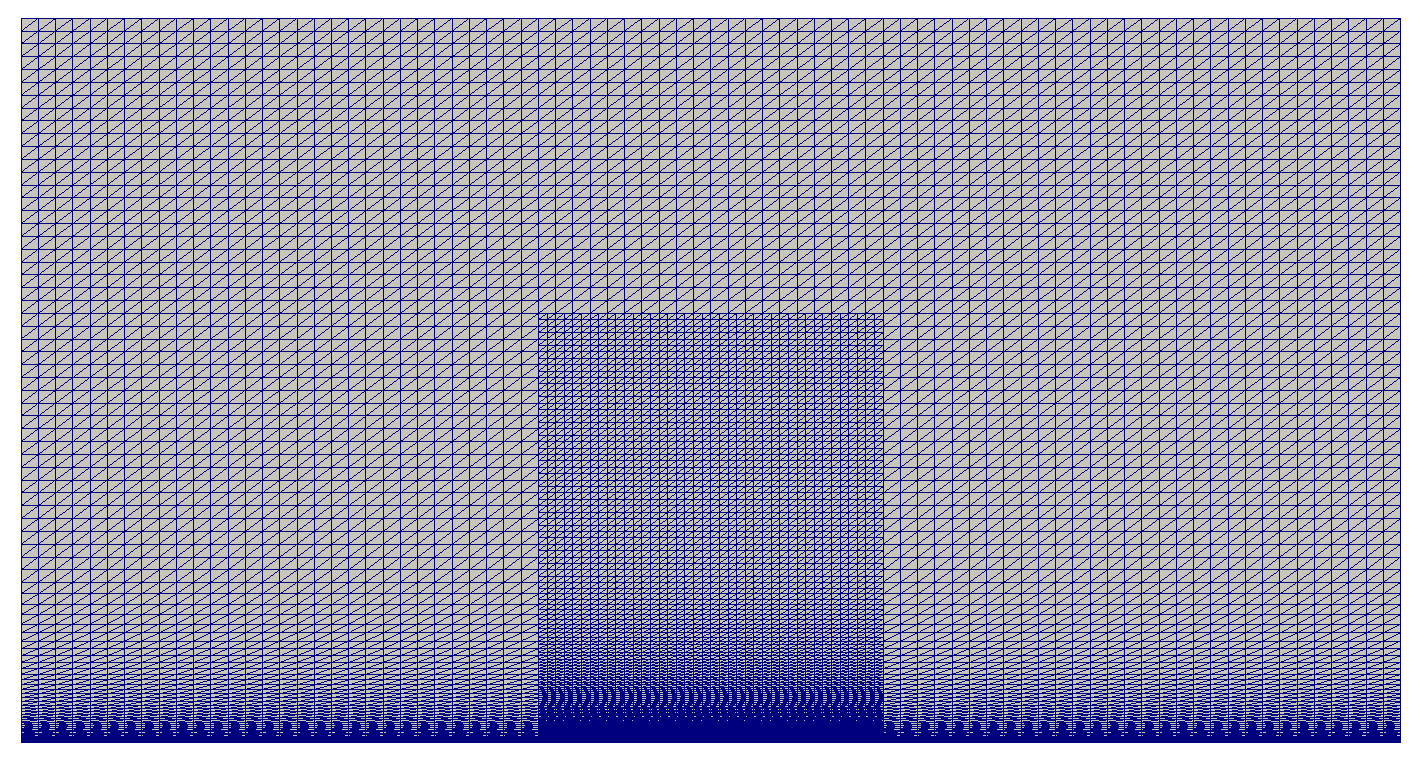
\includegraphics[width = 10 cm]{figs/meshing}
     \caption{Horizontal slide through the domain, to show a
     representative meshing. The single refinement region around the
     vanes is visible, along with the finer boundary layer mesh near the
     ground.}
     \label{fig:meshing}
    \end{center}
  \end{figure}

Finally, the diffusivities are proportionally
scaled with grid size to ensure that the cell Reynolds number, 
\begin{equation}
 \text{Re}_\text{cell} = \frac{\text{max}(\Delta x,\Delta y) u}{\nu_T}
\end{equation}
 is maintained for every simulation, to ensure stability.


%% hmin = 0.001  
%% hmax = 0.4  
%% zb = 2.0
%% hrat = ${/ ${mesh-options/hmax} ${mesh-options/hmin}}
%% zmax = ${mesh-options/domain_x3_max}
%% loghrat = ${= log ${mesh-options/hrat}}
%% c2 = ${/ ${mesh-options/zb} ${- ${mesh-options/hrat} 1}} 
%% zetab = ${/ ${mesh-options/zmax} ${+ 1 ${/ ${- ${mesh-options/zmax} ${mesh-options/zb}} ${* ${mesh-options/c2} ${mesh-options/hrat} ${mesh-options/loghrat}}}}}
%% c3 = ${/ ${mesh-options/loghrat} ${mesh-options/zetab}}
%% mesh_nx3 = ${= ceil ${/ ${* ${mesh-options/zmax} ${mesh-options/c2} ${mesh-options/c3}} ${mesh-options/hmin}}}
%% c1 = ${* ${mesh-options/c2} ${mesh-options/c3} ${= exp ${* ${mesh-options/c3} ${mesh-options/zetab}}}}
%% redistribute = '{x}{y}{if(z>${mesh-options/zetab},${mesh-options/c1}*(z-${mesh-options/zmax})+${mesh-options/zmax},${mesh-options/c2}*(exp(${mesh-options/c3}*z)-1))}' 

%After operation, solutions are evaluated to ensure that 
%the qualitative character of the solution does not change.

\section{Software Stack}

The numerical formulations described in Section~\ref{sec:discretization}
had been implemented using the GRINS library\cite{GRINSpaper} by Bauman
and Stogner using the Libmesh\cite{libMeshPaper} FEM infrastructure. It
was designed to support multiphysics FEM applications, the reusability
and extensibility of mathematical modeling kernels, supporting
interfaces to existing solver and discretization libraries to enable
modern solution strategies, while, at the same time, retaining
flexibility to effectively address a wide range of science and
engineering problems.   

GRINS provides a platform that enables powerful numerical algorithms
such as adjoint-based AMR, adaptive modeling, sensitivity analysis,
and, eventually, enabling uncertainty quantification. While few of these
capabilities are in use for the present work, they could be useful in
future investigations. 

GRINS stands for, ``General Reacting Incompressible Navier-Stokes'',
which roughly encapsulates the physical regimes it was originally
designed to simulate. GRINS is open-source, and available on
\hyperref[www.github.com/grinsfem/grins]{GitHub}. It is released 
under LGPL2.1.  GRINS is heavily unit tested, with over 60 tests
available to ensure the reliability of results regardless of install
platform. 

%The remainder of this section is devoted to
%discussing the underlying libraries used and the description of the
%GRINS framework.  

GRINS uses the fparser\cite{fparser}
library to support both parsing and compilation of mathematical
functions into high performance kernels. This capability allows for
easy specification of boundary conditions, initial conditions, or
constitutive equations from an input file. Some of these inputs are
detailed in Appendix~\ref{sec:archiving}. 

GRINS/Libmesh are built on the PETSC\cite{petsc} solver package, which
provides the numerical linear algebra packages used for constructing and
using sparse matrices, finding the iterative solution of linear systems,
and for preconditioning.  

While a variety of solver options have been tested in PETSC, all the
results shown in this document use GMRES with block Jacobi for
preconditioning\cite{Saad:2003} for the linear solve. This uses the
inverse of the diagonal block for that processor for preconditioning of
the entire linear system. In addition, a preconditioner is used for the
solution of the diagonal block. This is approximated with incomplete LU
factorization\cite{?}. Here, the ``incomplete'' refers
to the level of fill you use, with greater levels of fill approaching
the ``complete'' LU factorization. 

In principle, alternative software libraries/frameworks such as
FEniCS\cite{fenics}, OpenFOAM\cite{openfoam}, etc. would likely be
capable of simulating this regime. While these and other libraries have
various strengths and weaknesses, the pre-eminent concern is the parallel
performance at the intended processor count, due to the rapid
design iterations necessary for this research campaign. Given these concerns,
the GRINS library is a satisfactory tool. 

%% (11:41:54 AM) nick: ``-ksp_view -ksp_type gmres -pc_type bjacobi
%% -sub_pc_type ilu -sub_pc_factor_levels 0'' 
%% (11:42:00 AM) Paul Bauman: OK
%% (11:42:17 AM) Paul Bauman: -pc_type is the preconditioner for the entire linear system
%% (11:42:25 AM) Paul Bauman: You're doing bjacobi = block Jacobi
%% (11:42:28 AM) nick: right
%% (11:42:36 AM) nick: and does anyone have a good reference I can learn
%% this better? i feel as if I cant look this up, for some reason 
%% (11:42:39 AM) Paul Bauman: That is just using the inverse of the
%% diagonal block for that processor 
%% (11:42:46 AM) Paul Bauman: Now
%% (11:42:55 AM) Paul Bauman: that is a linear solve
%% (11:43:17 AM) Paul Bauman: So you can use all the linear solver
%% technology to solve or approximately that block 
%% (11:43:24 AM) Paul Bauman: Hence, -sub_pc_type
%% (11:43:32 AM) hil left the room.
%% (11:43:46 AM) Paul Bauman: That's the preconditioner it's going to
%% use to precondition the linear system for the solution of the
%% diagonal block 
%% (11:43:53 AM) Paul Bauman: You're telling it to use incomplete lu
%% (11:44:26 AM) Paul Bauman: Now the -sub_pc_factor_levels options
%% applies to ilu 
%% (11:44:28 AM) hil entered the room.
%% (11:44:44 AM) Paul Bauman: The incomplete part of imcomplete LU is
%% about the level of fill you use 
%% (11:45:05 AM) Paul Bauman: The more levels of fill you have, the more
%% ``complete'' the incomplete LU will be 
%% (11:45:08 AM) Paul Bauman: Does that make sense?
%% (11:45:23 AM) nick: no, that is where you lost me
%% (11:45:39 AM) nick: i dont think i know this level of fill
%% (11:46:17 AM) Paul Bauman: Check out Youssef Saad's book if more
%% curious about the subject 
%% (11:46:37 AM) nick: cool thanks
%% (11:46:38 AM) Paul Bauman: Suffice it to say, you heopfully shouldn't
%% ever need to go past 3 or 4 levels of fill 
%% (11:47:03 AM) Paul Bauman: Also, if you've got superlu installed with
%% the PETSc, consider using -sub_pc_factor_mat_solver_package superlu 
%% (11:47:15 AM) Paul Bauman: That's a *much* faster/better
%% implementation than PETSc's 

At the time of this writing, Grins has 94 regression tests, which
provides a reasonable degree of confidence in verification testing of
the library. Several of these tests directly test the capabilities in
GRINS used in this document. In particular, several of the tests were
contributed to GRINS directly by the Author during the course of this
work and the addition of several of the models detailed in
Chapter~\ref{sec:mathmodel}. 


\section{Tool Chain and Simulation Custodianship}

Simulations are performed on the Texas Advanced Computing Center\cite{?}
(TACC) supercomputers Lonestar Four and Stampede. Run durations for transient
cases are typically twelve hours to perform several hundred timesteps. 
The steady runs are considerably shorter, and require less
than ten minute runtimes. Typically  the wall clock times of the
steady-state runs are two or three minutes to solution. As a result, the
queue time is significantly longer than the actual production runtime. 
These runs are submitted to the production queue and are  
264-528 processing cores, or 22-44 nodes on Lonestar4 (with 12 cores per
node), and a similar number for Stampede. The runs have
several million degrees of freedom (DoF), and the local number of DoF
per core is maintained at $O(10^4)$. This was selected due to memory
constraints, after a strong scaling analysis of the performance of the
code on these resources, and after consulting with the software developers.  
At the time of this writing libMesh has been scaled to tens of thousands of
cores and has been run on over 100,000 cores on the BG/Q machine Mira at
Argonne National Lab\cite{libmesh-scaling}, and the scaling results here
are consistent with the performance expectations for this library.

In November, 2015, runs were also staged during early access into full
production period on TACC's new system, Lonestar5. This machine is
closer in terms of software stack to Stampede, using the Simple Linux
Utility for Resource Management (Slurm)\cite{?} scheduling
system.  

After a run terminates, several scripts are automatically invoked. 
These scripts archive the run (outside of the volatile /scratch 
production directories) and simultaneously, label the concluded run with
unique metadata that defines the system environment, the jobs input
files and run definitions, and information detailing the
hypothesis or physics the job was intended to investigate. Finally, once
a week a script performs \textbf{rsync} on the entire archived database to
ensure more than single redundancy for the runs. 

In other words, the workflow is designed to permit rapid queuing of a
series of runs (in parallel) to investigate a variety of conditions or
scenario parameters. This capability is necessary for the optimization
campaign detailed in Section~\ref{sec:results}, where running many
concurrent investigations are required to sample the configuration
space.  

%\section{Testing and Verification}
%grid convergence?


%The validation of the  runs is detailed in the next Chapter. 

\chapter[Characteristics of the Homogenized Boundary Layers\\ at Atmospheric Reentry-like Conditions]
        {Characteristics of the Homogenized Boundary Layers at Atmospheric Reentry-like Conditions}
\label{sec:bldata}

To reduce turbulence-driven uncertainty in aerothermodynamic heating predictions
for blunt-bodied reentry vehicles, new direct numerical simulations of
spatiotemporally homogenized boundary layers were performed to address the need
for high-quality turbulence model calibration data identified in
\autoref{sec:review}.
%
In this chapter, the characteristics of these new homogenized boundary layer
simulations are examined.
%
The chapter additionally provides enough information so that a
prediction-oriented practitioner may assess this new data's merit towards
inclusion in some calibration process.
%
The simulations will be described and analyzed, which includes
simulation details (\autoref{sec:bldata_details}), notes on the observed
integral boundary layer thicknesses (\autoref{sec:bldata_integrallengths}), turbulence
statistics (\autoref{sec:bldata_stats}), and Favre-averaged equation budgets
(\autoref{sec:bldata_budgets}).

For a more in-depth investigation of the homogenization see
\citet{Topalian2014Spatiotemporal}.
%
Also note that homogenization-related forcing terms from that reference must
be incorporated when calibrating a turbulence model using the present results.
The terms are not, however, required for subsequent use of a calibrated model.


%%%%%%%%%%%%%%%%%%%%%%%%%%%%%%%%%%%%%%%%%%%%%%%%%%%%%%%%%%%%%%%%%%%%%%%%%%%%%%
\section{Simulation Details}
\label{sec:bldata_details}

Two cold-wall boundary layers were simulated at conditions representative of
flow over the Orion MPCV thermal protection system at peak heating during
vehicle reentry from the International Space Station.
%
Additional background on the reentry conditions can be found in \autoref{sec:orionmpcv}.
%
The two scenarios of interest were constructed by taking conditions found 3.199
meters and 4.134 meters leeward of the stagnation point in
Figures~\ref{fig:cevisslam_summary1} and~\ref{fig:cevisslam_summary_fpg} and
then increasing the momentum Reynolds numbers $\Reynolds[\theta]{}$ to match
similar flow speeds in \autoref{tbl:BaumanCEVConditionsPerfect} as measured by
the edge Mach numbers $\Mach[e]{}$.
%
That is, the scenarios combined $\Reynolds[\theta]$ and $\Mach[e]{}$ from fully
turbulent conditions with fully laminar edge-to-wall temperature ratios
$T_e/T_w$, wall blowing velocities $v_w^+$, and pressure gradient strengths
$p_{e,\xi}^{\ast}$.
%
Relative to drawing from only the fully turbulent conditions in
Tables~\ref{tbl:BaumanCEVConditions} and~\ref{tbl:BaumanCEVConditionsPerfect},
these hybrid conditions produced larger $T_e/T_w$ and somewhat
milder favorable pressure gradients.
%
The choice of these conditions was motivated by the
work to be presented in \autoref{sec:relam}.
%
Though the resulting hybrid scenarios strictly speaking appear nowhere in the
fully turbulent simulations by \citet{Bauman2011Loose} or
\citet{Stogner2011Uncertainty}, the two scenarios meet
\citet{Settles1991Hypersonic}'s \emph{realistic test conditions} criterion,
discussed in \autoref{sec:datareq}, and are therefore suitable for
turbulence model calibration targeting this predictive context.

% Source data from production turbulent boundary layer summaries
%   5c9f94456104cf1772db023f246c2915  relam2.299.h5
%   805ac7be682012c0dd94c9159b5b671c  turb3.199.h5
%   7t45cad67daeb545189ac5ea3f6a4e27  turb4.134.h5

\begin{table}
\makecommand{\z}{\phantom{0}}  % Facilitates column alignment
\makecommand{\Z}{\phantom{.0}} % Ditto
\centering
\caption[Homogenized boundary layer simulations suitable for turbulence model calibration]{%
    Homogenized boundary layer simulations performed by Suzerain
    v0.1.6.34-r45407 intended for turbulence model calibration.
    %
    For all cases, $\textrm{Pr} = \mu C_p / \kappa = 0.7$, $\alpha=0$ in
    $\mu_B=\alpha\mu$, $\beta=\nicefrac{2}{3}$ in $\mu / \mu_0={\left(T /
    T_0\right)}^\beta$, and $\gamma = C_p / C_v = 1.4$.
    %
    Extents were $L_x/l_0=10$, $L_y/l_0=2.5$, $L_z/l_0=3$ employing a
    piecewise-quintic B-spline basis with $N_y$ collocation points stretched
    per the hyperbolic tangent parameter ``$\tanh$'' following~\eqref{eq:htstretch1}.
    %
    Grid spacings are normalized by $\delta_\nu = \mu_w / \rho_w / u_\tau$ where
    $u_\tau = \sqrt{\tau_w / \rho_w}$ and $\tau_w = \left(\mu \partial_y u\right)_w$.  The
    distance between the isothermal wall and the first and tenth collocation
    point is written $y_{1}^{+}$ and $y_{10}^{+}$,
    respectively.\label{tbl:table_turb_hbl}
}
{\renewcommand{\tabcolsep}{0.420em}
\begin{tabular}{cccccccccccc}
& \multicolumn{6}{c}{Code inputs} & \\ \cmidrule(lr){2-7}
Case             &
$\textrm{Re}$    &
$\textrm{Ma}$    &
$N_x$            &
$N_y$            &
$N_z$            &
$\tanh$          &
$\Delta{}x^{+}$  & % Details from post-processing
$y_{1}^{+}$      &
$y_{10}^{+}$     &
$\Delta{}z^{+}$  &
Turnovers
\\
\toprule\toprule
%Case   &  Re    &  Ma      &  Nx   &  Ny   &  Nz   &  tanh  &  x+    &  y+1   &  y+10  &  z+     &  Turnovers  \\
%q2.299 &  1100  &  0.6598  &  256  &  192  &  128  &  2.00  &  13.9  &  0.14  &  6.1   &  \z8.4  &  22.4       \\
 t3.199 &  2400  &  0.8985  &  512  &  256  &  256  &  2.25  &  13.9  &  0.14  &  6.1   &  \z8.4  &  \z6.4      \\
 t4.134 &  3250  &  1.1522  &  512  &  256  &  256  &  2.35  &  19.0  &  0.17  &  7.2   &  11.4   &  \z6.9
\end{tabular}}
\end{table}

%%%%%%%%%%%%%%%%%%%%%%%%%%%%%%%%%%%%%%%%%%%%%%%%%%%%%%%%%%%%%%%%%%%%%%%%%%%%%%
%%%%%%%%%%%%%%%%%%%%%%%%%%%%%%%%%%%%%%%%%%%%%%%%%%%%%%%%%%%%%%%%%%%%%%%%%%%%%%

\begin{table}[p]
\centering
\caption[Scenario parameters for homogenized boundary layer simulations]{%
    Input parameters and resulting homogenized boundary layer
    conditions.  $\textrm{Re}_{99}$ and $\textrm{Ma}_{99}$
    computed from conditions at $\delta_{99}$.  To properly account
    for a nonuniform base flow, $\text{Re}_\theta$ is defined
    per~\eqref{eq:momreynolds_general}.  Wall blowing velocity $v_w^{+}
    = v_w / u_\tau$.\label{tbl:table_turb_hbl_params}
    %Case
    %q2.299 treated all directions linearly implicitly using a time step safety
    %factor of 0.20.
}
{\renewcommand{\tabcolsep}{0.388em}
\begin{tabular}{cccccccccc}
& \multicolumn{3}{c}{Code inputs} & \\ \cmidrule(lr){2-4}
Case                                           &
$\operatorname{gr}_{t_0}\!\left(\Delta\right)$ &
$T_w/T_0$                                      &
$v_w/u_0$                                      &
$\delta_{99}/l_0$                              &
$\textrm{Re}_{99}$                             &
$\textrm{Re}_{\theta}$                         &
$\textrm{Ma}_{99}$                             &
$T_{99}/T_w$                                   &
$v_w^{+}$
\\
\toprule\toprule
%Case   &  grdelta  &  Tw      &  vw             &  delta99  &  Re_delta99  &  Re_theta  &  Ma_99   &  ratio_T  &  vwallplus      \\
%q2.299 &  0.0100   &  0.2391  &  \num{2.64e-4}  &  1.146    &  1293        &  184       &  0.6598  &  4.107    &  \num{8.98e-3}  \\
 t3.199 &  0.0135   &  0.2346  &  \num{2.30e-4}  &  1.001    &  2468        &  382       &  0.9041  &  4.128    &  \num{8.52e-3}  \\
 t4.134 &  0.0200   &  0.2333  &  \num{1.90e-4}  &  1.002    &  3346        &  531       &  1.1523  &  4.201    &  \num{7.18e-3}
\end{tabular}}
\end{table}

%%%%%%%%%%%%%%%%%%%%%%%%%%%%%%%%%%%%%%%%%%%%%%%%%%%%%%%%%%%%%%%%%%%%%%%%%%%%%%
%%%%%%%%%%%%%%%%%%%%%%%%%%%%%%%%%%%%%%%%%%%%%%%%%%%%%%%%%%%%%%%%%%%%%%%%%%%%%%

\begin{table}[p]
\centering
\caption[Pressure gradients in homogenized boundary layer simulations]{%
    Pressure gradient strengths for the simulated boundary layers.
    %
    The inviscid base flow was constructed per
    Appendix~\ref{sec:radialflow} using inputs $\delta/l_0=1$, $\gamma$,
    $\textrm{Ma}_{e}=\textrm{Ma}$ from \autoref{tbl:table_turb_hbl}
    and $p_{e,\xi}^{\ast}$.
    %
    Observations of $p_{{99},\xi}^{\ast}$, Launder's acceleration
    parameter $K$~\citep{Launder1964Laminarization},
    the Pohlhausen parameter~$K_s$, and parameter
    $\Lambda_n$~\citep{Narasimha1979Relaminarization} are shown evaluated
    as defined in \autoref{fig:cevisslam_summary_fpg} taking $\delta_{99}$
    to be the boundary layer edge.\label{tbl:table_turb_hbl_fpg}
}
{%\renewcommand{\tabcolsep}{0.395em}
\begin{tabular}{ccccccc}
& \multicolumn{1}{c}{Code input} & \\ \cmidrule(lr){2-2}
Case                                      &
\raisebox{0.10ex}{$p_{e,\xi}^{\ast}$}     &
\raisebox{0.10ex}{$p_{{99},\xi}^{\ast}$}  &
$K,\mu=\mu_{99}$                          &
$K,\mu=\mu_w$                             &
$K_s$                                     &
$\Lambda_n$
\\
\toprule\toprule
%Case   &  target          &  p_ex            &  Launder_e       &  Launder_w       &  Pohlhausen  &  Lambda_n  \\
%q2.299 &  \num{-0.01269}  &  \num{-0.01452}  &  \num{1.136e-5}  &  \num{4.438e-6}  &  19.00       &  3.902     \\
 t3.199 &  \num{-0.01019}  &  \num{-0.01025}  &  \num{4.176e-6}  &  \num{1.623e-6}  &  25.44       &  3.345     \\
 t4.134 &  \num{-0.01234}  &  \num{-0.01233}  &  \num{3.734e-6}  &  \num{1.434e-6}  &  41.81       &  4.113
\end{tabular}}
\end{table}

%%%%%%%%%%%%%%%%%%%%%%%%%%%%%%%%%%%%%%%%%%%%%%%%%%%%%%%%%%%%%%%%%%%%%%%%%%%%%%
%%%%%%%%%%%%%%%%%%%%%%%%%%%%%%%%%%%%%%%%%%%%%%%%%%%%%%%%%%%%%%%%%%%%%%%%%%%%%%

\begin{table}
% Assuming "a" is a summary file, this computes Nusselt number per Redmine #2563
% which seems to jive with Schlicting equation 4.16.
% a['bl.thick'].attrs['delta99'] * a['bar_T_{y'].attrs['mu'][0] / (a['bl.edge99'].attrs['T'] - a['bl.wall'].attrs['T'])}
\centering
\makecommand{\z}{\phantom{0}}  % Facilitates column alignment
\makecommand{\Z}{\phantom{.0}} % Ditto
\makecommand{\n}{\phantom{-}}  % Ditto
\centering
\caption[Edge vs. wall conditions in homogenized boundary layer simulations]{%
    Edge versus wall conditions in the simulated boundary layers.  Friction
    quantities $\mathrm{Re}_\tau = \delta_{99} / \delta_\nu$, $\textrm{Ma}_\tau
    = u_\tau / a_w = u_\tau / \sqrt{T_w}$, and $c_f = 2 \tau_w /
    \left(\rho_{99} u_{99}^2\right)$.  Nondimensional heat flux $B_q = -
    \mu_w \left(\partial_y T\right)_w  / \left(\textrm{Pr}\,\rho_w u_\tau
    T_w\right)$~\citep{Bradshaw1977Compressible} and local Nusselt number
    $\mathrm{Nu}_{99} = \delta_{99} \left(\partial_y T\right)_w /
    \left(T_{99} - T_w\right)$.\label{tbl:table_turb_hbl_edgewall}
}
{\renewcommand{\tabcolsep}{0.425em}
\begin{tabular}{ccccccccc}
Case               &
$\rho_{99}/\rho_w$ &
$\mu_{99}/\mu_w$   &
$v_{99}/v_w$       &
$\textrm{Re}_\tau$ &
$\textrm{Ma}_\tau$ &
$c_f$              &
$-B_q$             &
$\textrm{Nu}_{99}$
\\
\toprule\toprule
%Case   &  rho99/rho_w  &  mu99/mu_w  &  v99/v_w      &  Re_tau  &  Ma_tau   &  cf              &  -Bq       &  Nusselt  \\
%q2.299 &  0.2445       &  2.560      &  $-25.75\z$   &  408     &  0.04028  &  \num{7.443e-3}  &  0.09635   &  \z8.895  \\
 t3.199 &  0.2427       &  2.573      &  $-\z3.003$   &  714     &  0.05008  &  \num{6.128e-3}  &  0.09765   &  15.59\z  \\
 t4.134 &  0.2383       &  2.603      &  $\n30.95\z$  &  976     &  0.06311  &  \num{5.994e-3}  &  0.1018\z  &  21.74\z
\end{tabular}}
\end{table}


One direct numerical simulation was performed at each scenario of interest.  The
coordinate system is depicted in \autoref{fig:geometry}.
Tables~\ref{tbl:table_turb_hbl}--\ref{tbl:table_turb_hbl_edgewall}
document the two scenarios,
for reproducibility
distinguishing between code input parameters and \emph{a posteriori} observations.
These tables will be discussed in more detail below.  The
calculations used the Navier--Stokes formulation from \autoref{sec:goveqn}
equipped with the ``slow growth'' spatiotemporal homogenization of
\autoref{sec:imposing_fpg}.  Favorable pressure gradients were obtained by
supplying an inviscid base flow, constructed as described in
Appendix~\ref{sec:radialflow}, to the spatiotemporal model.  The continuous
equations were discretized following \autoref{sec:techniques} and implemented in
Suzerain as described by \autoref{sec:software}.  Simulation data
has been archived per Appendix~\ref{sec:archiving}.

\autoref{tbl:table_turb_hbl} reports the target $\Reynolds$ and $\Mach$ based on
boundary layer edge conditions for each simulation, along with the domain sizes
and numerical resolutions used.
%
The nondimensional formulation in conjunction with the inviscid
base flow design procedure \emph{a priori} causes $\rho_{99}
/ \rho_0$, $u_{99} / u_0$, $\delta_{99} / l_0$, and $T_{99} /
T_0$ to all be approximately one so that code inputs $\textrm{Re}
\approx \rho_{99} u_{99} \delta_{99} / \mu_{99}$ and $\textrm{Ma}
\approx u_{99} / a_{99}$.  The slow growth
parameter $\operatorname{gr}_{t_0}\!\left(\Delta\right)$ was tuned to obtain
$\delta_{99}/l_0\approx{}1$ as an operational convenience.  As a result,
for either scenario and for
any length $L$ it holds that $L / l_0 \approx L / \delta_{99}$ to
within 0.2\%.  The streamwise domain extent normalized by the boundary
layer thickness was taken 25\% larger than the value of eight employed by
\citet{Guarini2000Direct} because they reported their choice was mildly
too small.  The spanwise extent approximately matches that used by
\citet{Spalart1988Direct}.  Grid resolution in the streamwise and
spanwise directions is similar to the cold-wall channel simulations by
\citet{Coleman1995Numerical} listed in \autoref{tbl:table_channel}.

% COMPARE ColemanJFM1995 Figure 1, Guarini JFM 2000 Figure 1
\begin{figure}
\centering
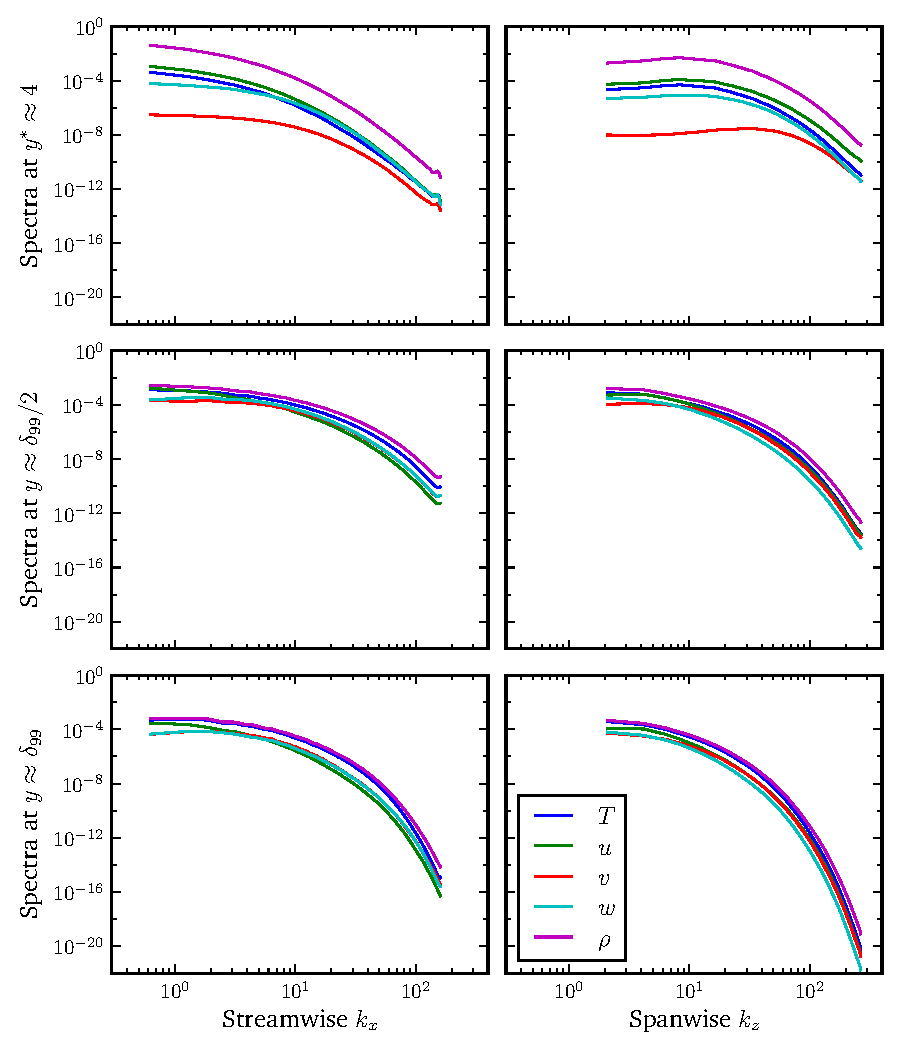
\includegraphics[width=\textwidth]{spectra-turb3199}
\caption{%
    One-dimensional, unnormalized Fourier energy spectra for case
    t3.199.\label{fig:spectra-t3199}
}
\end{figure}

% COMPARE ColemanJFM1995 Figure 1, Guarini JFM 2000 Figure 1
\begin{figure}
\centering
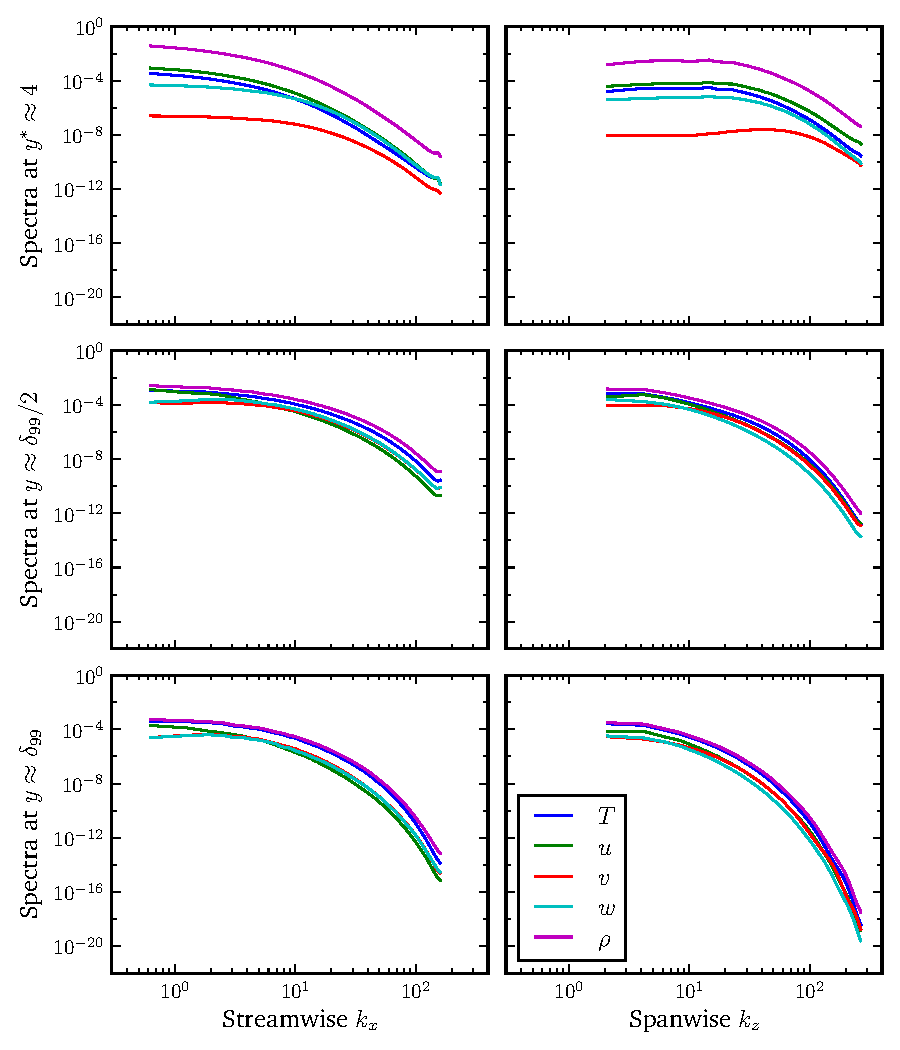
\includegraphics[width=\textwidth]{spectra-turb4134}
\caption{%
    One-dimensional, unnormalized Fourier energy spectra for case
    t4.134.\label{fig:spectra-t4134}
}
\end{figure}

% COMPARE ColemanJFM1995 Figures 3-4, Guarini JFM 2000 Figure 2
\begin{figure}
\centering
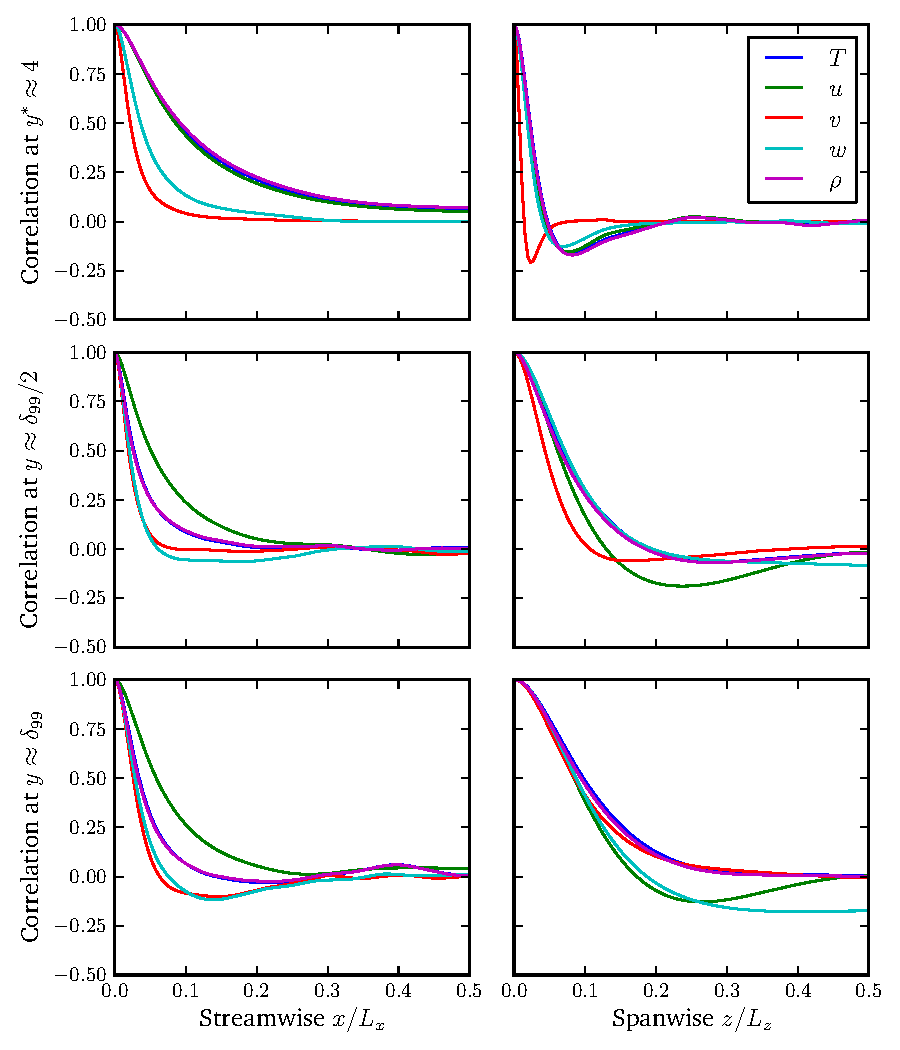
\includegraphics[width=\textwidth]{autocorr-turb3199}
\caption{%
    Two-point correlations for simulation t3.199.\label{fig:autocorr-t3199}
}
\end{figure}

% COMPARE ColemanJFM1995 Figures 3-4, Guarini JFM 2000 Figure 2
\begin{figure}
\centering
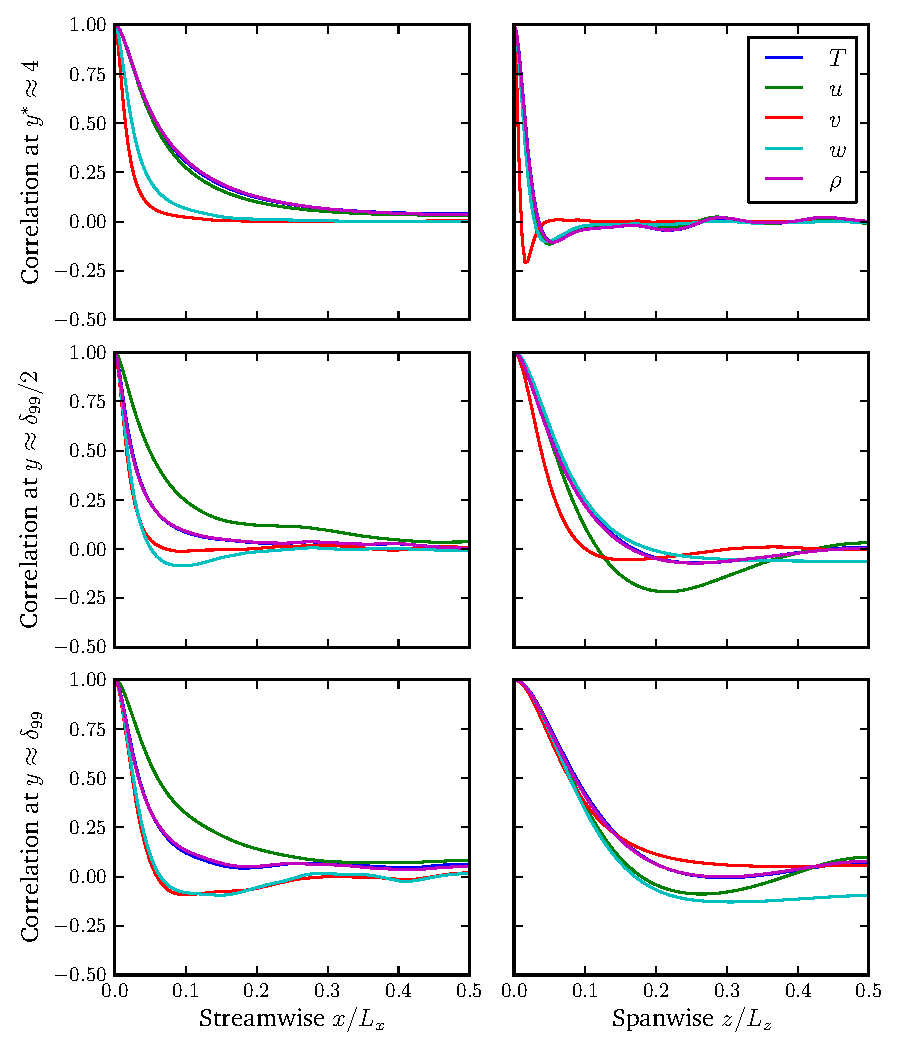
\includegraphics[width=\textwidth]{autocorr-turb4134}
\caption{%
    Two-point correlations for simulation t4.134.\label{fig:autocorr-t4134}
}
\end{figure}

The one-dimensional Fourier spectra, shown for primitive variables in
Figures~\ref{fig:spectra-t3199} and~\ref{fig:spectra-t4134}, indicate that the
present simulations are better resolved in the periodic directions than
those of \citeauthor{Coleman1995Numerical}.
%
The streamwise spectra at $y^{\ast}=y \sqrt{\tau_w / \rho} / \nu \approx{}4$ demonstrate that $L_x$ was
slightly smaller than required to eliminate artifacts from the periodic boundary
conditions.  This is corroborated by the two-point correlations in
Figures~\ref{fig:autocorr-t3199} and~\ref{fig:autocorr-t4134} which show $T$,
$u$, and $\rho$ not decorrelating fully at $x/L_x=0.5$.  However, the streamwise
correlations exhibit less coherence than those of
\citeauthor{Coleman1995Numerical} and \citeauthor{Guarini2000Direct} and, like
those authors, we anticipate finite domain effects to have little impact on the
results presented here.  Aside from the spanwise velocity~$w$, spanwise
coherence far from the wall is smaller than \citeauthor{Guarini2000Direct}
reported and is found acceptable.
%
The increase in $w$ correlation as $y$ increases, also observed by
Victor Topalian (personal communication), is thought to be a benign artifact of the
homogenization.
%
Given the quality of the spectra, evidently $L_z$ could have been larger without
incurring extra computational expense and without adversely decreasing spanwise
resolution.

In the wall-normal direction for case t3.199, collocation point
$y_{15}^{+}\approx{}10.4$, 178~points were inside $\delta_{99}$,
and $\left.\Delta{}y^{+}\right|_{y=\delta_{99}} \approx 10.7$.
For case t4.134, $y_{13}^{+}\approx{}10.1$, 180~points were inside
$\delta_{99}$, and $\left.\Delta{}y^{+}\right|_{y=\delta_{99}}
\approx 15.0$.  To account for the considerable density and
temperature gradients arising from holding wall temperatures
fixed, the wall-normal grid spacings are more appropriately
assessed when scaled by semi-local units~\citep{Huang1995Compressible,Morinishi2005Study}
%
which use either $u^\ast_\tau = \sqrt{\tau_w / \rho}$ or $\delta^\ast_\nu = \nu / u^\ast_\tau$.
%which are similar to
%$\delta_\nu$ and $u_\tau$ except that local density and viscosity are used in
%lieu of wall values.
For simulation t3.199, collocation point
$y_{27}^{*}\approx{}10.1$ and $\left.\Delta{}y^{*}\right|_{y=\delta_{99}}
\approx 1.6$.  For case t4.134, $y_{24}^{*}\approx{}10.3$ and
$\left.\Delta{}y^{*}\right|_{y=\delta_{99}} \approx 2.2$.

Both simulations used linear implicit time discretization only for
operators involving derivatives in the wall-normal direction and,
given the lessons learned in \autoref{sec:channel_runs} regarding the
aggressiveness of the eigenvalue estimates from \autoref{sec:wallnormaleigval},
time step safety factors of 0.35 were selected.  As measured by
time-to-solution, linear implicitness in three directions was equally but no
more performant than the wall-normal-only variant.  The latter was chosen as it
used smaller time steps and therefore was expected to better resolve flow
dynamics.  The column ``turnovers'' conveys the time over which the statistical
ensemble was collected divided by $\delta_{99}/u_\tau$.  The ensemble for cases
t3.199 and t4.134 includes 764 and 837 instantaneous planar averages over $x$
and $z$ which were collected \emph{in situ} from the simulations.  Uncertainties
were estimated from the temporal trace of these equispaced samples following
procedures outlined in \autoref{eq:uqaccounting}.

\autoref{tbl:table_turb_hbl_params} documents the fixed temporal slow growth
rates $\operatorname{gr}_{t_0}\!\left(\Delta\right)$, the isothermal wall
temperatures, and the wall blowing rates.  It shows that the homogenization held
$\delta_{99} \approx 1$ and that the desired $\Reynolds[99]$ and $\Mach[99]$
conditions were produced.  The remaining columns confirm that simulations t3.199
and t4.134 indeed correspond to their namesake locations in
Figures~\ref{fig:cevisslam_summary1} and~\ref{fig:cevisslam_summary_fpg} save
for possessing $\Reynolds[\theta]$ representative of those found in in
\autoref{tbl:BaumanCEVConditionsPerfect}.

\autoref{tbl:table_turb_hbl_fpg} characterizes the favorable pressure gradients
found in the two simulations in a variety of ways.  The desired
inviscid pressure gradient parameter $p_{e,\xi}^\ast$, defined in \eqref{eq:defnpexi},
is listed alongside the observed result at $\delta_{99}$ labeled
$p_{99,\xi}^{\ast}$.  The inviscid base flow design procedure from
Appendix~\ref{sec:radialflow} produced the target pressure gradient strength to
within 0.6\%.  Comparing the tabulated values against
\autoref{fig:cevisslam_summary_fpg}, the simulated values of Launder's
acceleration parameter $K$ are between the bands shown calculated from fully
laminar Orion MPCV computations.  Simulation t3.199 shows reasonable agreement
with the expected Pohlhausen parameter $K_s$ from the same figure while
simulation t4.134 is more than 50\% too large.  However, the $K_s$ values
computed from the MPCV source data are suspect as they possess appreciable numerical
artifacts.  Both simulations produced $\Lambda_n$ values roughly a factor of two
less than the MPCV data but the discrepancy is not surprising as the wall shear
$\tau_w$ entering into $\Lambda_n$ was not specified \emph{a priori}.
We consider the inviscid base design procedure to be successful because it
closely reproduced the desired condition on $p_{99,\xi}^\ast$ while yielding
pressure gradients not too dissimilar from the MPCV data when quantified using
other metrics.

\autoref{tbl:table_turb_hbl_edgewall} conveys several quantities of interest
from the simulations.  As expected, the prescribed wall temperatures $T_w/T_0$
produce larger densities and lower viscosities near the wall.
%
Despite its wall-normal velocity at the edge being positive, simulation t4.134
uses subsonic inflow boundary conditions because of how the homogenization
causes inputs $L_y$ and $\operatorname{gr}_{t_0}\!\left(\Delta\right)$ to modify
the wall-normal inviscid characteristics as discussed in
\autoref{sec:impacthomovisc}.
%
On account of wall injection, friction Reynolds
number $\Reynolds[\tau]{}$ is higher and skin friction $c_f$ is lower than
might be expected based upon $\Reynolds[\theta]{}$ and
$\Mach[99]{}$~\citep{Sumitani1995Direct, Smits2005Turbulent}.  To ease
comparing surface heating predictions against the present results, the
nondimensional heat flux $B_q$ and the Nusselt number $\textrm{Nu}_{99}$
%based on $T_{99}$ and $T_w$
are also tabulated.

%%%%%%%%%%%%%%%%%%%%%%%%%%%%%%%%%%%%%%%%%%%%%%%%%%%%%%%%%%%%%%%%%%%%%%%%%%%%%%
\section{A Note on Integral Thicknesses and the Clauser Parameter}
\label{sec:bldata_integrallengths}

The omissions of the displacement thickness $\delta^\ast$, the momentum
thickness $\theta$, and the Clauser parameter
$\beta$~\citep{Clauser1954Turbulent} from the above tables merit explanation.
That explanation requires revisiting the classical definitions of the two
thicknesses to properly account for the presence of the nonuniform inviscid
base flows which were used to enforce nonzero pressure gradients.  Along the
way, the two related integral thickness Reynolds numbers accommodating
nonuniform base flows will be derived.

As explained in, for example, \citet[\textsection{}9.2]{Dowling2012} the
displacement thickness $\delta^\ast$ is the distance by which the wall would
have to be displaced upward in a hypothetical frictionless flow to maintain the
same mass flux as that in the viscous flow.  That is, $\delta^\ast$ is the
length satisfying
\begin{align}
    \int_0^\infty {\rho u}_\text{viscid} (y) \, \mathrm{d}y
&=
    \int_{\delta^\ast}^\infty {\rho u}_\text{inviscid} (y) \, \mathrm{d}y.
\end{align}
Formally the upper limit may be replaced by any sufficiently large, finite
value because ${\rho u}_\text{viscid} \to {\rho u}_\text{inviscid}$ as
$y\to\infty$.  Assuming our domains are large enough,
\begin{align}
    \int_0^{L_y} {\rho u}_\text{viscid} (y) \, \mathrm{d}y
&=
    \int_{\delta^\ast}^{L_y} {\rho u}_\text{inviscid} (y) \, \mathrm{d}y.
    \label{eq:dispthick_general}
\end{align}
One can obtain a simplification often taken as a definition~\citep[Equation
10.95]{Schlichting2000Boundary},
\begin{align}
    \delta^\ast
&=
    \int_0^{L_y} 1 - \frac{{\rho u}_\text{viscid} (y)}{\rho_e u_e} \, \mathrm{d}y,
    \label{eq:dispthick_const}
\end{align}
for the special case of a uniform inviscid flow where ${\rho u}_\text{inviscid}
(y) = \rho_e u_e$.
%
Multiplying by $\rho_e u_e / \mu_e$, recognizing the displacement Reynolds
number $\Reynolds[\delta^\ast]{}$, and formally converting back to the
nonuniform inviscid base flow,
\begin{align}
    \Reynolds[\delta^\ast]{}
=
    \frac{\rho_e u_e \delta^\ast}{\mu_e}
&=
    \frac{\rho_e u_e}{\mu_e}
    \int_0^{L_y} 1 - \frac{{\rho u}_\text{viscid} (y)}{\rho_e u_e} \, \mathrm{d}y,
\notag\\&=
    \mu_e^{-1}
    \int_0^{L_y} \rho_e u_e - {\rho u}_\text{viscid} (y) \, \mathrm{d}y,
\notag\\&\approx
    \mu_e^{-1}
    \int_0^{L_y} {\rho u}_\text{inviscid}(y) - {\rho u}_\text{viscid} (y) \, \mathrm{d}y.
    \label{eq:dispreynolds_general}
\end{align}
A constant viscosity, here chosen to be $\mu_e$, should scale the
above integral when defining $\Reynolds[\delta^\ast]{}$.  There is no sensible
way to incorporate dimensions of inverse viscosity into its integrand's left
term thus permitting $\mu^{-1}(y)$ to multiply the right term.

\begin{figure}
\centering
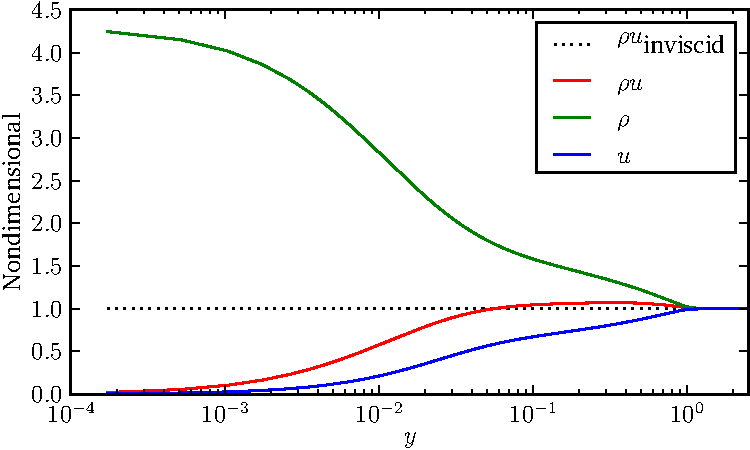
\includegraphics[]{delta1weird}
\caption{%
    The inviscid base flow and viscous flow profiles for simulation
    t4.134\label{fig:delta1weird}
}
\end{figure}

Mean profiles from simulation t4.134 pictured in \autoref{fig:delta1weird} are
the impetus for recalling the general displacement thickness
balance~\eqref{eq:dispthick_general} as well as its
simplification~\eqref{eq:dispthick_const}.  Progressing from the cold wall at
$y=0$ to the boundary layer edge at $y=\delta_{99}\approx{}1$, the streamwise
velocity increases, the density drops considerably, and the momentum in the
viscous flow exceeds that of the inviscid base flow.
%
Evaluating integral~\eqref{eq:dispthick_const} taking $\rho_e u_e$ from
$\delta_{99}$ produces $\delta^\ast/l_0 = -0.03923$.
%
Interpreting this negative $\delta^\ast$ through the usual displacement effect
intuition, for simulation t4.134 introducing the cold plate into the inviscid
profile increases the mass flow rate because it significantly increases the
near-wall density.
%
Negative $\delta^\ast$ are reported for exotic flows but
seem uncommon~\citep[e.g.][]{Fergason2001Simulations, Brown1952Solutions}.
%
The flow, however, need not be exotic.  The zero-pressure-gradient boundary
layer forming on a sufficiently cold, flat plate in laminar air will exhibit a
negative displacement thickness (Truman E. Ellis, personal communication).
%
Evaluating the right hand integrand for the more correct
balance~\eqref{eq:dispthick_general} behaves unusually--- the shape of the inviscid base flow when $y < 0$ does not
influence the viscous solution on $y\in\left[0,L_y\right]$ but it
impacts $\delta^\ast$.
%
%%% To elaborate, in the ``subsurface'' region where $y<0$ any
%%% ${\rho u}_\textrm{inviscid} (y)$ from a stationary solution
%%% of the inviscid Euler equations is admissible provided that
%%% the solution agrees with the chosen base flow at finitely many
%%% collocation points $y_l\in\left[0,L_y\right]$.  This ability to
%%% freely choose the subsurface inviscid profile and thereby, on a
%%% fixed computational grid, adjust $\delta^\ast$ without consequences
%%% perhaps surprisingly makes $\delta^{\ast} < 0$ somewhat ill-defined
%%% per~\eqref{eq:dispthick_general}.
%
For this reason, a generalization of~\eqref{eq:dispthick_const},
\begin{align}
    \delta^\ast
&=
    \int_0^{L_y} 1 - \frac{{\rho u}_\text{viscid} (y)}
                          {{\rho u}_\text{inviscid} (y)} \, \mathrm{d}y,
    \label{eq:dispthick_final}
\end{align}
is selected as a definition and evaluating it shows
$\delta^\ast = -0.03918$ in simulation t4.134.
%
Therefore, $\Reynolds[\delta^\ast]$ must be negative and indeed
evaluating~\eqref{eq:dispreynolds_general} finds $\Reynolds[\delta^\ast] =
-129$.
%
The Clauser parameter $\beta=\frac{\delta^\ast}{\tau_w} \frac{\partial
p}{\partial x}=0.1608$ is positive in this favorable pressure gradient flow,
contrary to expectations~\citep[e.g.][]{Bowersox1996Turbulence}, because of
negative displacement effects.
%
Simulation t3.199 also exhibits the actual momentum exceeding the inviscid
profile momentum (not shown) but possesses $\delta^\ast/l_0=0.006429$,
$\Reynolds[\delta^\ast]=15.8$, and $\beta=-0.02148$;  $\beta$
in no way communicates the strength of the pressure gradient as many
authors term 0.1 a strong magnitude~\citep{Smith1994Effects,Luker2000Influence}.

Negative displacement effects are not evident in the reacting, fully
turbulent Orion MPCV data from~\autoref{tbl:BaumanCEVConditions}
($\delta^\ast/\delta\approx 0.113$) nor do they appear in the fully
laminar results depicted in \autoref{fig:cevisslam_summary_fpg} ($\beta<0$
leeward of the stagnation point).  These effects might not occur because
of the higher edge Prandtl numbers in those reacting simulations (see
$\Prandtl[e]$ in \autoref{fig:cevisslam_summary1}) because as the Prandtl number
increases it causes the thermal boundary layer to grow more slowly relative to
the momentum boundary layer.

The momentum thickness $\theta$ quantifies the momentum defect relative to the
inviscid flow after removing displacement effects.  That is, $\theta$ is the
length satisfying
\begin{align}
    \int_0^{L_y} {\rho u^2}_\text{viscid} (y) \, \mathrm{d}y
&=
    \int_{\theta}^{L_y}  {\rho u^2}_\text{inviscid} (y) \, \mathrm{d}y
  - \int_0^{\delta^\ast} {\rho u^2}_\text{inviscid} (y) \, \mathrm{d}y
    \label{eq:momthick_general}
\end{align}
given fixed $\delta^\ast$ where again the upper limit has been truncated to
the domain extent.
%
The commonly seen degenerate form of the above balance, often taken as a
definition when ${\rho u}_\text{inviscid} (y) = \rho_e u_e$, is recovered as
follows:\footnote{%
    \citet[page 214]{Smits2005Turbulent} and \citet[page
    324]{LiepmannRoshko2002} present result~\eqref{eq:momthick_incomp}.
    \citet[Equation 10.95]{Schlichting2000Boundary} made an
    error in their definition for $\theta$.
}
\begin{align}
    \int_0^{L_y} {\rho u^2}_\text{viscid} (y) \, \mathrm{d}y
&=
    \rho_e u_e^2 \left(L_y - \theta\right)
  - \rho_e u_e^2 \delta^\ast
\notag\\
    \rho_e u_e^2 \theta
&=
    \rho_e u_e^2 L_y
  - \int_0^{L_y} {\rho u^2}_\text{viscid} (y) \, \mathrm{d}y
  - u_e \left[\rho_e u_e \delta^\ast\right]
\notag\\
&=
    \int_0^{L_y} \rho_e u_e^2 - {\rho u^2}_\text{viscid} (y) \, \mathrm{d}y
  - u_e \left[
        \int_0^{L_y} \rho_e u_e - {\rho u}_\text{viscid} (y) \, \mathrm{d}y
    \right]
\notag\\
    \theta
&=
    \int_0^{L_y}
        \left(1 - \frac{{\rho u^2}_\text{viscid} (y)}{\rho_e u_e^2}
    \right)  \, \mathrm{d}y
  - \int_0^{L_y}
        \left(1 - \frac{{\rho u}_\text{viscid} (y)}{\rho_e u_e}
    \right)  \, \mathrm{d}y
\notag\\
&=
    \int_0^{L_y} \frac{{\rho u}_\text{viscid} (y)}{\rho_e u_e} \left(
        1 - \frac{{u}_\text{viscid} (y)}{u_e}
    \right)  \, \mathrm{d}y
    \label{eq:momthick_incomp}.
\end{align}
Unlike the analogous~\eqref{eq:dispthick_const}, only nonnegative values
are possible.
%
%\citet[\textsection{}9.2]{Dowling2012} provides the interpretation that, in
%this special case, $\rho_e u_e^2 \theta$ is nothing but the momentum loss in
%the viscous flow because of the presence of the boundary layer.
%
Multiplying by $\rho_e u_e/\mu_e$ and formally converting back to the nonuniform
base flow,
\begin{align}
    \Reynolds[\theta]{}
=   \frac{\rho_e u_e \theta}{\mu_e}
&=  \frac{\rho_e u_e       }{\mu_e}
    \int_0^{L_y} \frac{{\rho u}_\text{viscid} (y)}{\rho_e u_e} \left(
        1 - \frac{{u}_\text{viscid} (y)}{u_e}
    \right)  \, \mathrm{d}y
\notag\\
&=  \mu_e^{-1}
    \int_0^{L_y} {\rho u}_\text{viscid} (y) \left(
        1 - \frac{{u}_\text{viscid} (y)}{u_e}
    \right)  \, \mathrm{d}y
\notag\\
&\approx  \mu_e^{-1}
    \int_0^{L_y} {\rho u}_\text{viscid} (y) \left(
        1 - \frac{{u}_\text{viscid} (y)}{u_\text{inviscid} (y)}
    \right)  \, \mathrm{d}y.
    \label{eq:momreynolds_general}
\end{align}
Here, $\mu(y)$ could have been incorporated into the integrand, but it
was not for consistency with~\eqref{eq:dispreynolds_general}.

Defining $\theta$ via the general balance~\eqref{eq:momthick_general} is
problematic when negative displacement effects are present because, for
consistency, that approach should use $\delta^\ast$ from~\eqref{eq:dispthick_general}.
%
For this reason, generalizing~\eqref{eq:momthick_incomp} the present work uses
\begin{align}
    \theta
&=
    \int_0^{L_y} \frac{{\rho u}_\text{viscid} (y)}
                      {{\rho u}_\text{inviscid}(y)} \left(
        1 - \frac{{u}_\text{viscid} (y)}{u_\text{inviscid}(y)}
    \right)  \, \mathrm{d}y
\end{align}
and finds $\theta=0.1557$ and $\theta=0.1611$ for simulations t3.199 and t4.134,
respectively.  The generalization makes little difference--- assuming the base
flow was constant and directly evaluating~\eqref{eq:momthick_incomp} from
inviscid values at $y=\delta_{99}$ changes only the final reported digit in each
result.
%
Computed either way, the two spatiotemporal simulations have momentum
thicknesses larger than the reacting, fully turbulent Orion MPCV data
from~\autoref{tbl:BaumanCEVConditions} ($\theta/\delta\approx 0.134$).
%
The present simulation shape factors $H=\delta^\ast/\theta$ of $0.04129$ and
$-0.2432$ are well below standard turbulent boundary layer values and contrast
strongly with the fully turbulent MPCV result of $H\approx0.847$ acquired with
the aid of a Baldwin--Lomax model.
%
Momentum Reynolds numbers computed according
to~\eqref{eq:momreynolds_general} appeared in
\autoref{tbl:table_turb_hbl_params}.


%%%%%%%%%%%%%%%%%%%%%%%%%%%%%%%%%%%%%%%%%%%%%%%%%%%%%%%%%%%%%%%%%%%%%%%%%%%%%%


% Wall injection tends to activate near-wall turbulence, shear stress, heat fluxes \citet{Sumitani1995Direct}
% Injection stimulates the occurrence of quasicoherent streamwise vorticle structures which are associated with primary turbulence mechanisms \citet{Sumitani1995Direct}

%Turbulent Mach Number

\section{Turbulence Statistics}
\label{sec:bldata_stats}

This section reviews a collection of turbulent statistics for the present
simulations.  Comparisons to other work are included but are limited
because, as evidenced by their shape factors, these two cold-wall
spatiotemporally homogenized flows differ considerably from canonical boundary
layers.


\begin{figure}
\centering
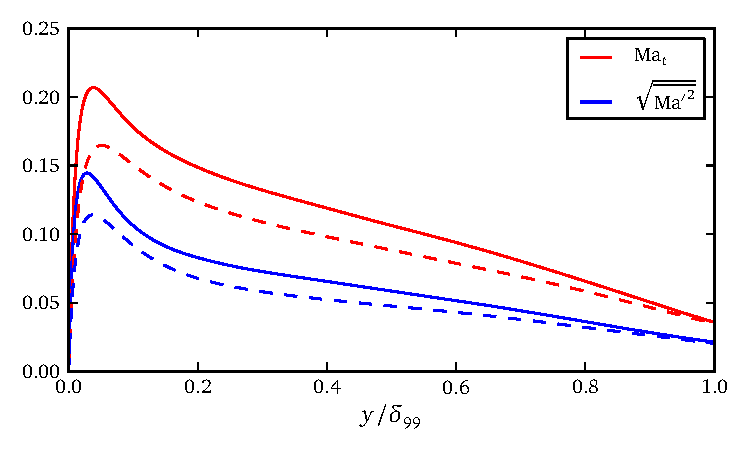
\includegraphics[]{hqd_mach}
\caption[Fluctuating Mach number profiles for simulations t3.199 and t4.134]{%
    Turbulent Mach number $\Mach[t]=\sqrt{2 k}/\bar{a}$
    and root-mean-squared local Mach number for simulations
    t3.199 (dashed) and t4.134 (solid).\label{fig:hdq_mach}
}
\end{figure}

\autoref{fig:hdq_mach} reports the turbulent Mach number $\Mach[t]{}$ and
root-mean-squared Mach number fluctuations.  Turbulence in both simulations
should only be weakly affected by compressibility effects because $\Mach[t]$ is
well below 0.3~\citep{Smits2005Turbulent}.  Local shocklets are not expected and
so the smoothness assumptions inherent to the numerical approach
from~\autoref{sec:techniques} are valid.  Consistent with
\citet{Guarini2000Direct}, the peak $\Mach[t]$ is slightly offset from the
root-mean-square profile because the former includes contributions from all
three velocity components while the latter uses only streamwise information.  On
this plot, and on the remainder of the plots in this section using abscissa
$y/\delta_{99}$, simulation t4.134 shows sharper near-wall gradients because its
$\Reynolds[\theta]$ is larger than simulation t3.199.  Peak magnitudes for
simulation t4.134 match a $\Mach[e]=1.2$ and $\Reynolds[\theta]{}=420$ simulation by
\citet{Topalian2014Temporal} employing temporal
homogenization~\eqref{eq:temporalhomogenization} and also targeting Orion MPCV
cold, blowing wall conditions.  The introduction of spatial homogenization terms
within the model seems to have no impact on these curves.

\begin{figure}[p]
\centering
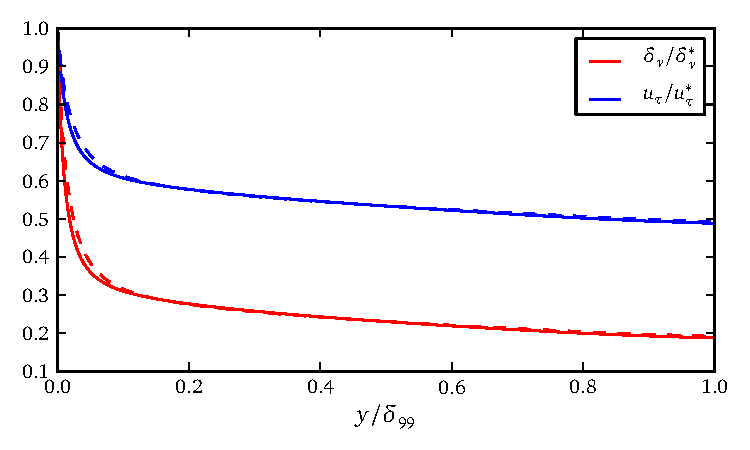
\includegraphics[]{hqd_star}
\caption[Wall versus semi-local scaling for simulations t3.199 and t4.134]{%
    Comparison of viscous length and velocity scales using wall and
    semi-local units~\citep{Huang1995Compressible} in simulations t3.199
    (dashed) and t4.134 (solid).\label{fig:hdq_star}
}
\end{figure}

\begin{figure}
\centering
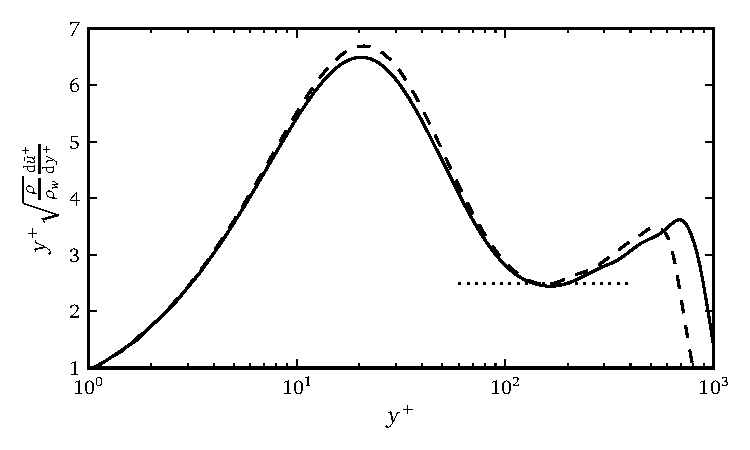
\includegraphics[]{hqd_inner}
\caption[Examination of inner scaling in simulations t3.199 and t4.134]{%
    Examination of inner scaling in simulations t3.199
    (dashed) and t4.134 (solid).
    For
    reference, the horizontal line shows $1/\kappa$ for
    $\kappa=0.40$.\label{fig:hdq_inner}
}
\end{figure}

Though compressibility is weak, \autoref{fig:hdq_star} shows that for these
large $T_{99}/T_w$ ratios variable density effects are strongest near the wall and
they continue throughout the boundary layer.  This is consistent with
$\Prandtl{}=0.7<1$ and the earlier discussion of very small or negative
displacement effects.  \autoref{fig:hdq_inner} shows an inner scaling plot
appropriate for compressible boundary layers~\citep{Chassaing2010Variable}.  In
a logarithmic inner region, one anticipates $\sqrt{\frac{\bar{\rho}}{\rho_w}}
\frac{\partial{\bar{u}^{+}}}{\partial y^{+}} = \frac{1}{\kappa y^{+}}$ which
does not appear because of the modest $\Reynolds[\theta]{}$ in these
simulations.  A von K\'arm\'an constant $\kappa$ of 0.40 predicts the tangent
where a logarithmic region would be expected at higher $\Reynolds[\theta]{}$.
In accordance with these two plots, semi-local units primarily will be used in
the remainder of the chapter.

Figures~\ref{fig:profile-t3199} and~\ref{fig:profile-t4134} show
nondimensional mean profiles and Reynolds stresses with the latter in semi-local
units.  The horizontal axes in the upper and lower images in the figures align
so that one can visually translate from $y^\ast$ to $y/\delta_{99}$.  Based on
techniques from \autoref{eq:uqaccounting}, uncertainties in the mean profiles
are presented in the upper right of each figure.  Qualitatively the uncertainty
profiles are similar between the two simulations though t3.199 shows somewhat
higher near-wall and mid-layer values and downward trends are more pronounced as
$y/\delta_{99}\to{}1$ in t4.134.  The peak uncertainties are modestly higher in
the higher $\Reynolds[\theta]$ case.  Importantly, the time step safety factor used
in these simulations did not produce the near-wall jaggedness that was visible
in~\autoref{fig:basic3k15} and so the temporal resolution is not suspect.
Turning to the lower half of the figure, the lower $\Mach[99]{}$ t3.199 shows a
slightly larger maximum $\widetilde{{u^{\prime\prime}}^2}$.  Maximum values are
higher than those found by \citet[Figure 6]{Guarini2000Direct} and
\citet[Figure 18]{Coleman1995Numerical} which is consistent with wall
blowing~\citep{Sumitani1995Direct}.  Uncertainties in the fluctuating quantities
grow as the edge of the boundary layer is approached but that is attributed to
the normalization by the small mean value found there.

Similar uncertainty estimates for over 225 Reynolds averaged scalar quantities
and their wall-normal derivatives were generated from \emph{in situ}
instantaneous averages taken over the streamwise and spanwise directions.  They
are not presented in this document but are available for calibration or modeling
purposes per Appendix~\ref{sec:archiving}.

\begin{figure}
\centering
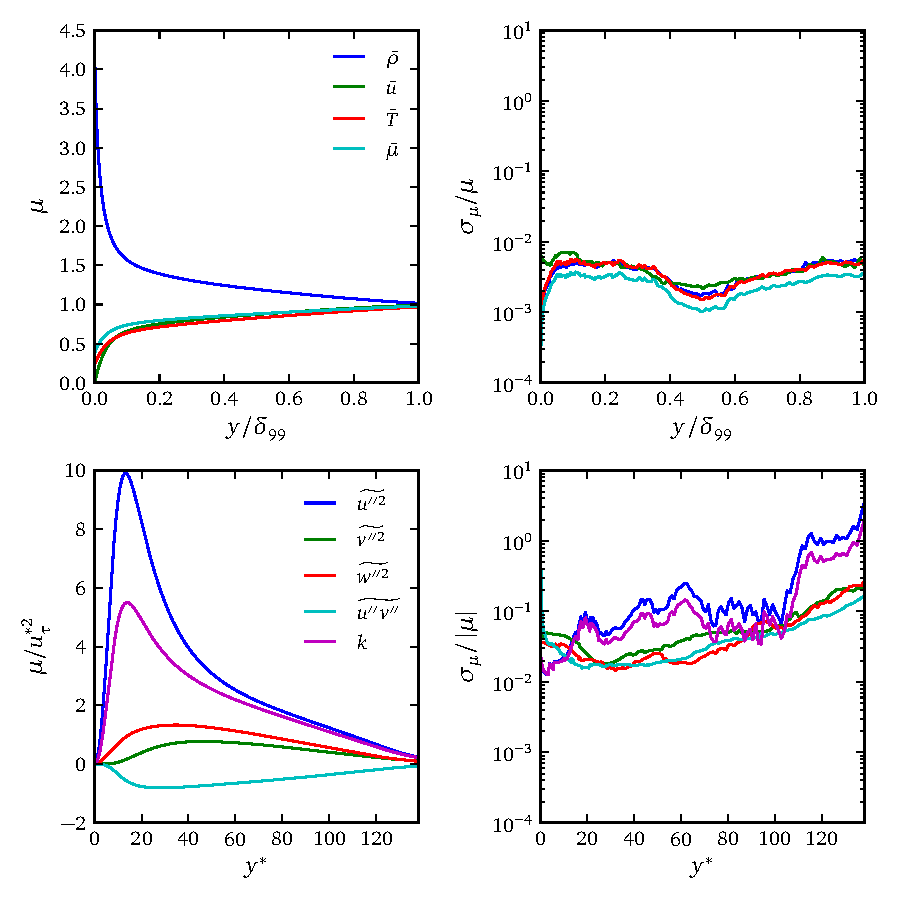
\includegraphics[width=\textwidth]{profile-t3199}
\caption[Profiles with quantified uncertainty for simulation t3.199]{%
    Reynolds-averaged primitive profiles (upper left) and Favre-averaged
    Reynolds stresses (lower left) with estimated standard errors
    as a fraction of mean (upper right, lower right) for simulation
    t3.199.\label{fig:profile-t3199}
}
\end{figure}

\begin{figure}
\centering
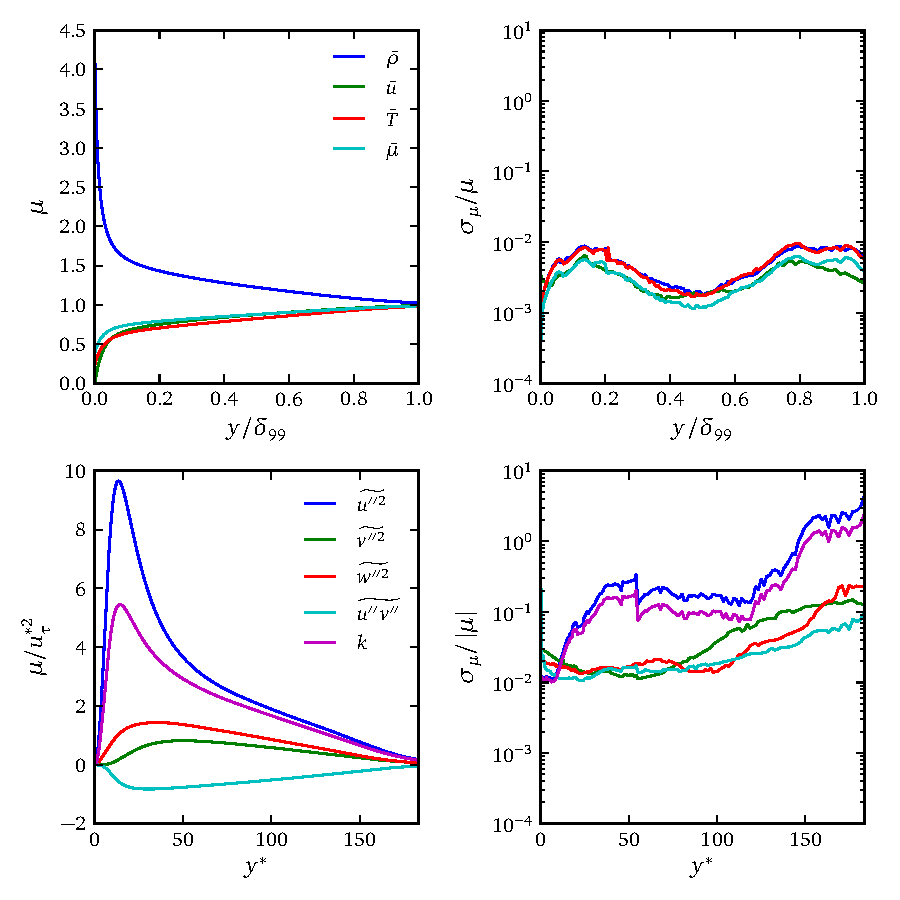
\includegraphics[width=\textwidth]{profile-t4134}
\caption[Profiles with quantified uncertainty for simulation t4.134]{%
    Reynolds-averaged primitive profiles (upper left) and Favre-averaged
    Reynolds stresses (lower left) with estimated standard errors
    as a fraction of mean (upper right, lower right) for simulation
    t4.134.\label{fig:profile-t4134}
}
\end{figure}

\begin{figure}[p]
\centering
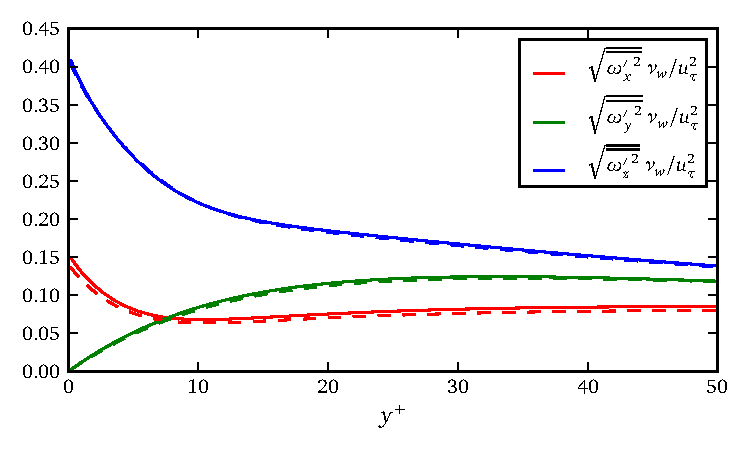
\includegraphics[]{hqd_vort}
\caption[RMS vorticity fluctuations for simulations t3.199 and t4.134]{%
    Root-mean-squared vorticity fluctuations normalized in wall units for
    simulations t3.199 (dashed) and t4.134 (solid).\label{fig:hdq_vort}
}
\bigskip\medskip
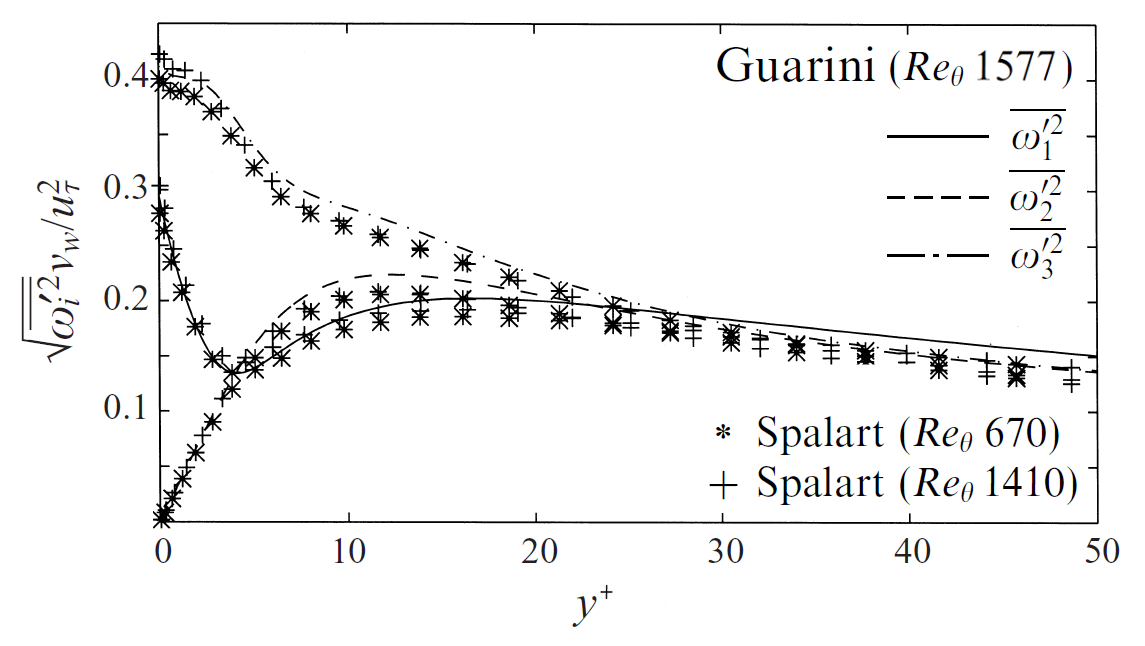
\includegraphics[width=5.2in]{GuariniJFM2000Figure8_Reworked}\hspace{1.5em}
\caption[RMS vorticity fluctuations reproduced from \citeauthor{Guarini2000Direct}]{%
    Root-mean-squared vorticity fluctuations from a $\Mach = 2.5$,
    adiabatic-wall spatially homogenized boundary layer by
    \citeauthor{Guarini2000Direct} and incompressible results by
    \citet{Spalart1988Direct}.  Reproduced from
    \citet{Guarini2000Direct}.\label{fig:hdq_vort_repo}
}
\end{figure}

\begin{figure}
\centering
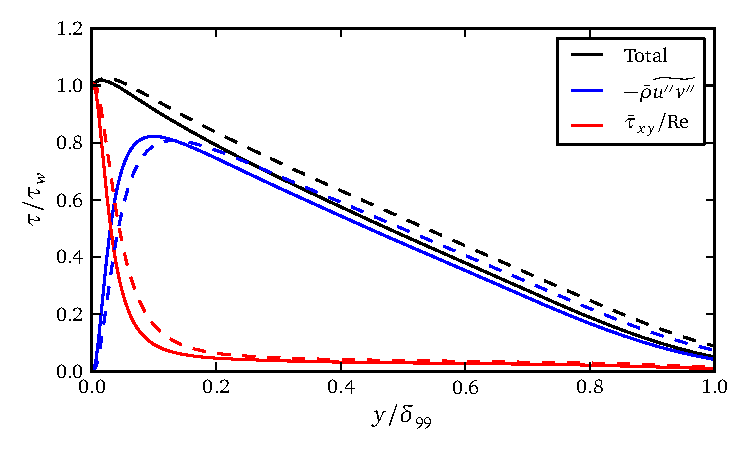
\includegraphics[]{hqd_tauxy}
\caption[Total shear stress contributions in simulations t3.199 and t4.134]{%
    Total shear stress contributions normalized in wall units for
    simulations t3.199 (dashed) and t4.134 (solid).\label{fig:hdq_tauxy}
}
\end{figure}

\autoref{fig:hdq_vort} displays root-mean-square vorticity fluctuations near the
wall normalized in wall units following \citet{Guarini2000Direct}.  Semi-local
units also caused the curves
to collapse for $y^{+}\lessapprox{}15$
in simulations t3.199 and t4.134
but they were less effective far from the wall (not shown).
Neither scaling removed the offset between the two simulations appearing in the
streamwise vorticity.  The spanwise maximum at the wall matches that shown in
\citet{Guarini2000Direct}, reproduced in \autoref{fig:hdq_vort_repo}.
The streamwise wall value is half what they
reported.  Qualitatively, the shapes have fewer curvature changes for
$y^{+}<20$, the near-wall local minimum in the streamwise data is more shallow,
and no localized peak appears in the wall-normal fluctuations.
These changes suggest the present simulations have atypical streamwise
vortex structures, perhaps as a consequence of wall blowing but the
spatiotemporal homogenization may also play a role.

\autoref{fig:hdq_tauxy} contains the total stress contributions for the streamwise
momentum equation.  The near-wall maxima are due to wall
injection~\citep{Sumitani1995Direct} with simulation t3.199 being slightly
higher because of its 18\% larger $v_w^{+}$.  \citet{Topalian2014Temporal},
using temporal homogenization~\eqref{eq:temporalhomogenization} in a
zero-pressure-gradient simulation at $\Mach[e]{}=1.2$ and
$\Reynolds[\theta]{}=420$, observed a blowing-related total stress maximum of
roughly 1.2 for a $v_w^{+}$ roughly
2.6x that used in simulation t4.134.  In contrast, t4.134 has maximum 1.0175.
The reduced maxima, relative to what might be expected if one scaled using only the blowing velocity,
are believed to be a consequence of the pressure gradient.

\begin{figure}
\centering
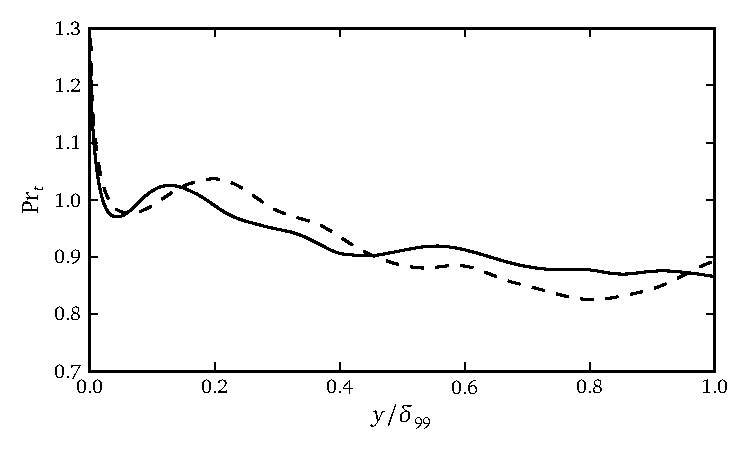
\includegraphics[]{hqd_prt}
\caption[Turbulent Prandtl number in simulations t3.199 and t4.134]{%
    Turbulent Prandtl number $\Prandtl[t]{} =
    \frac{\widetilde{u^{\prime\prime}v^{\prime\prime}}\partial_y\tilde{T}}
         {\widetilde{T^{\prime\prime}v^{\prime\prime}}\partial_y\tilde{u}}$
    for simulations t3.199 (dashed) and t4.134 (solid).\label{fig:hdq_prt}
}
\end{figure}

\autoref{fig:hdq_prt} reports the turbulent Prandtl number $\Prandtl[t]{}$ The
data shows perhaps unsettling waviness but similar fluctuations were observed
by \citet[Figure 14]{Guarini2000Direct}.  However, away from the wall the
present $\Prandtl[t]{}>0.8$ differs from their 0.7 result.

\begin{figure}[p]
\centering
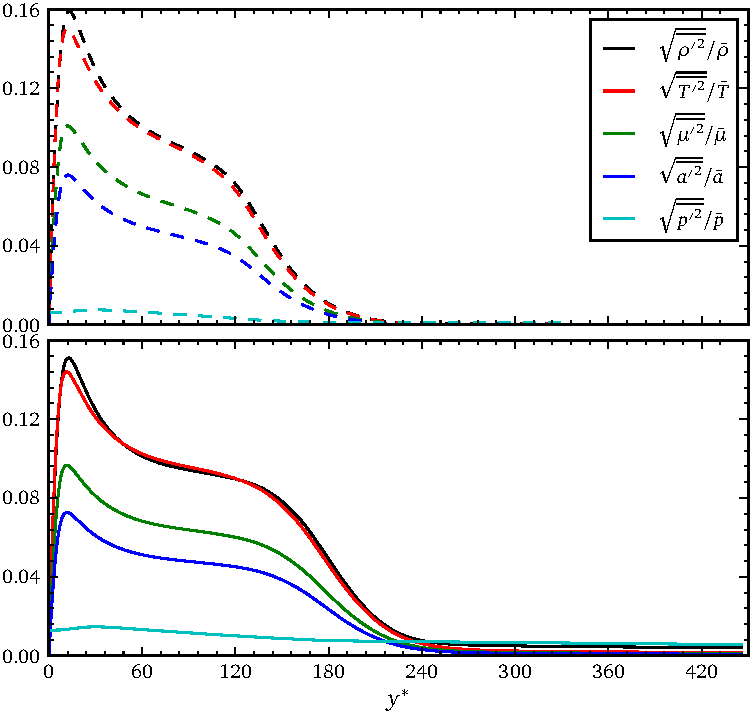
\includegraphics[]{hqd_fprop}
\caption[RMS thermodynamic fluctuations in simulations t3.199 and t4.134]{%
    Root-mean-squared thermodynamic property fluctuations normalized by local
    means for simulations t3.199 (above, dashed) and t4.134 (below,
    solid).\label{fig:hdq_fprop}
}
%\end{figure}
%\begin{figure}
%\centering
\bigskip\medskip
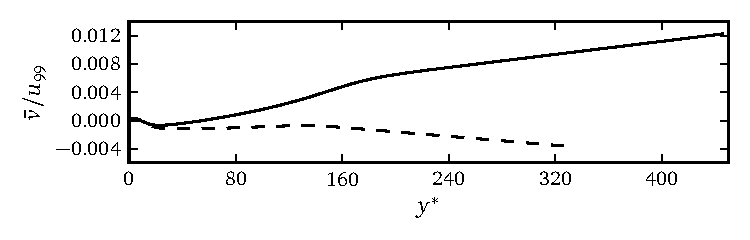
\includegraphics[]{hqd_v}
\caption[Mean wall-normal velocity for simulations t3.199 and t4.134]{%
    Mean wall-normal velocity normalized by the streamwise edge velocity
    for simulations t3.199 (dashed) and t4.134 (solid).\label{fig:hdq_v}
}
\end{figure}

\autoref{fig:hdq_fprop} contrasts root-mean-squared thermodynamic property
fluctuations between the two simulations.  Simulation t3.199 unexpectedly has
larger maxima than 4.134 for all quantities save pressure.
%
Most striking about these fluctuation magnitudes is that, unlike t3.199, in
t4.134 the pressure and density curves do not decay as fully outside
the boundary layer.
%
A fundamental difference between the inviscid base flow designs is one cause for
this behavioral change.  Simulation t3.199 is subsonic and therefore a favorable
pressure gradient is achieved, per Appendix~\ref{sec:radialflow}, with a
converging radial nozzle.  Supersonic simulation t4.134 uses a diverging radial
nozzle.

The mean wall-normal velocity $\bar{v}$ for these cases is shown in
\autoref{fig:hdq_v}.  The positive $\bar{v}$ at the wall quickly turns negative
in both simulations.  For t3.199 it stays negative thereafter causing
$\overline{\rho{}v}$ to become negative by $y/\delta_{99}\approx{}0.9$ (not
shown).  In t4.134, $\bar{v}$ changes sign before $y^\ast=80$ and proceeds to
increase throughout the upper portions of the domain with an appreciable curvature
change at the edge of the boundary layer.  At $y=L_y$ the wall-normal velocity
is more than 1\% of $u_{99}$ and $\overline{\rho v}$ is everywhere positive (not
shown).

A second potential cause for this lack of decay is the spatiotemporal
homogenization, possibly in conjunction with the numerical isothermal wall
and/or nonreflecting freestream boundary treatments.
%
It was noticed and subsequently confirmed by Topalian that, unlike
the temporal homogenization~\eqref{eq:temporalhomogenization}, the
spatiotemporal homogenization causes small point-to-point oscillations to appear
in the second derivative of pressure near both the lower and upper boundaries
(not shown).
%
This behavior can be reproduced by time-stepping a stationary one-dimensional
laminar solution even in zero-pressure-gradient cases for which the inviscid
base flow terms are inactive.
%
Transferring such a solution to progressively finer grids will cause the
pressure oscillations to eventually pollute other quantities and the numerical
solution to diverge.
%
Notably, only supersonic problems seem to be so affected.  Setting the modeled
defect growth rates (see \autoref{sec:imposing_fpg}) to be zero delays but does
not prevent the divergence.  The issue is not believed to be related to the
implicit treatment as time-stepping with fully explicit operators also shows
the same issue.
%
However, at wall-normal resolutions like that used for case t4.134 the precursor
pressure oscillations remain small and are not thought to spoil that
simulations' results.
%
Still, they suggest that, while suitable for calibration purposes and gross
behavioral investigations like those pursued in the next chapter, the
spatiotemporal homogenization and accompanying numerics in their current form
may not be appropriate for some studies of fundamental physics in supersonic
flows.

%%%%%%%%%%%%%%%%%%%%%%%%%%%%%%%%%%%%%%%%%%%%%%%%%%%%%%%%%%%%%%%%%%%%%%%%%%%%%%
\section{Favre-Averaged Equation Budgets}
\label{sec:bldata_budgets}

The spatiotemporal homogenization by \citet{Topalian2014Spatiotemporal} is
sufficiently new that term-by-term contributions to the averaged governing
equations, often called budgets, have not appeared in the literature.
%
This section presents such budgets, per the Favre-averaged Navier--Stokes
formulation documented in \autoref{sec:statevo}, to help quantify the impact of
this slow growth forcing on mean flow profiles.
%
Simulations t3.199 and t4.134 are particularly interesting for this purpose
because they fully exercise the novel inviscid base flow capabilities of the
homogenization.
%
In addition to characterizing the impact of the homogenization, this data
provides detailed information about the dynamics of complex boundary layers.

To begin, \autoref{fig:fans_rho} shows the budget for the Favre-averaged density~\eqref{eq:fans_mass}.  Though somewhat mundane, its presentation serves
three purposes.  First, it exhibits several choices made throughout the
remainder of this section.  Subsonic simulation t3.199 appears on the upper half
of the image with supersonic case t4.134 below.  Both halves use identical
ordinate ranges to communicate term-by-term budgets normalized by wall units.
Semi-local abscissa are chosen so that the two cases collapse permitting
comparisons of extrema locations between the upper and lower halves of the
figure.  The reader may find Figures~\ref{fig:profile-t3199}
and~\ref{fig:profile-t4134} helpful if converting locations from $y^\ast$ to
$y/\delta_{99}$ is desired.  A
logarithmic scale was selected so that near-wall, edge, and freestream behaviors of
the slow growth formulation can be assessed with one plot.  Second, \autoref{fig:fans_rho}
demonstrates several qualitative differences between the sub- and supersonic
behavior of the spatiotemporal formulation equipped with a favorable pressure
gradient inviscid base flow.  The subsonic case shows slow forcing, $\Ssd_\rho$,
changing sign inside the boundary layer while the supersonic forcing does not.
The boundary layer edge is quite apparent in the figure and $\Ssd_\rho$ changes
curvature dramatically in its vicinity.  Third, supporting comments in the last
section that the supersonic case is somewhat ill-behaved at the freestream
boundary, a kink appears only in the lower plot near $y=L_y$.

Figures~\ref{fig:fans_rho_u} and~\ref{fig:fans_rho_v} show budgets for
the two nontrivial scalar components of the Favre-averaged momentum~\eqref{eq:fans_mom}.  \autoref{fig:fans_rho_u}
demonstrates that $\Ssd_{\rho u}$ behaves similarly to $\Ssd_{\rho}$ with
regard to sub- versus supersonic conditions.  At $y^{\ast}\approx{}10$
simulation t4.134 shows a mildly more pronounced slow growth forcing peak and
again slight boundary condition artifacts at the freestream.  Slow growth makes
an appreciable contribution to the streamwise momentum balance
near the wall.  Turning to wall-normal momentum in
\autoref{fig:fans_rho_v}, the homogenization is not active and the subsonic and
supersonic cases are quite similar.

\autoref{fig:fans_rho_E} breaks apart the Favre-averaged total energy~\eqref{eq:fans_energy}.
Aside from anticipated Mach number-related
differences in viscous heating, the two simulations appear similar for
$y^\ast<40$.  Above that cutoff, slow growth and convection are much more active
in the supersonic case as a consequence of trends already shown in
\autoref{fig:hdq_v}.

Finally, the turbulent kinetic energy~\eqref{eq:fans_tke} appears for simulation
t3.199 in \autoref{fig:tke_t3199} and for t4.134 in \autoref{fig:tke_t4134}.
The upper half of each figure shows terms that strongly impact turbulent kinetic
energy $\rho k$.  The lower halves contain fine details that the upper plotting scale
would not permit visualizing.  The pressure dilatation and Reynolds heat
flux appear almost perfectly juxtaposed against one another because~\eqref{eq:lelecompresibility} was
used to eliminate the unclosed correlation $\overline{p'u''}$ from
formulation~\eqref{eq:fans_tke}.  The two terms are also summed in the lower
half.  As compared against a peak production of roughly 0.25 reported by
\citet{Schlatter2009Turbulent} for a spatially evolving zero-pressure-gradient
case at $\Reynolds[\theta]{}=670$, the present peak production is unexpectedly small
given that wall injection tends to energize
turbulence~\citep{Sumitani1995Direct}.
%
Importantly, Figures~\ref{fig:tke_t3199} and~\ref{fig:tke_t4134} demonstrate
that the \citet{Topalian2014Spatiotemporal} spatiotemporal homogenization
leaves the near-wall $\rho k$ budget largely unaffected.  The direct slow forcing
contribution $\overline{\Ssd_{\rho u}\cdot{}u^{\prime\prime}}$ is of the same
order of magnitude as the pressure terms for the present Mach numbers.

That last finding supports the expectation that a turbulence model calibrated to
accurately reproduce data from simulations t3.199 and t4.134 would be suitable
for use in predicting spatially evolving boundary layers with similar
characteristics.  Confirming this expectation by calibrating and validating
turbulence models is outside the scope of the current work.

\todo[inline]{%
    Fix weird figure size variability in the following figures---
    matplotlib padding is being finicky.
}

\begin{figure}
\centering
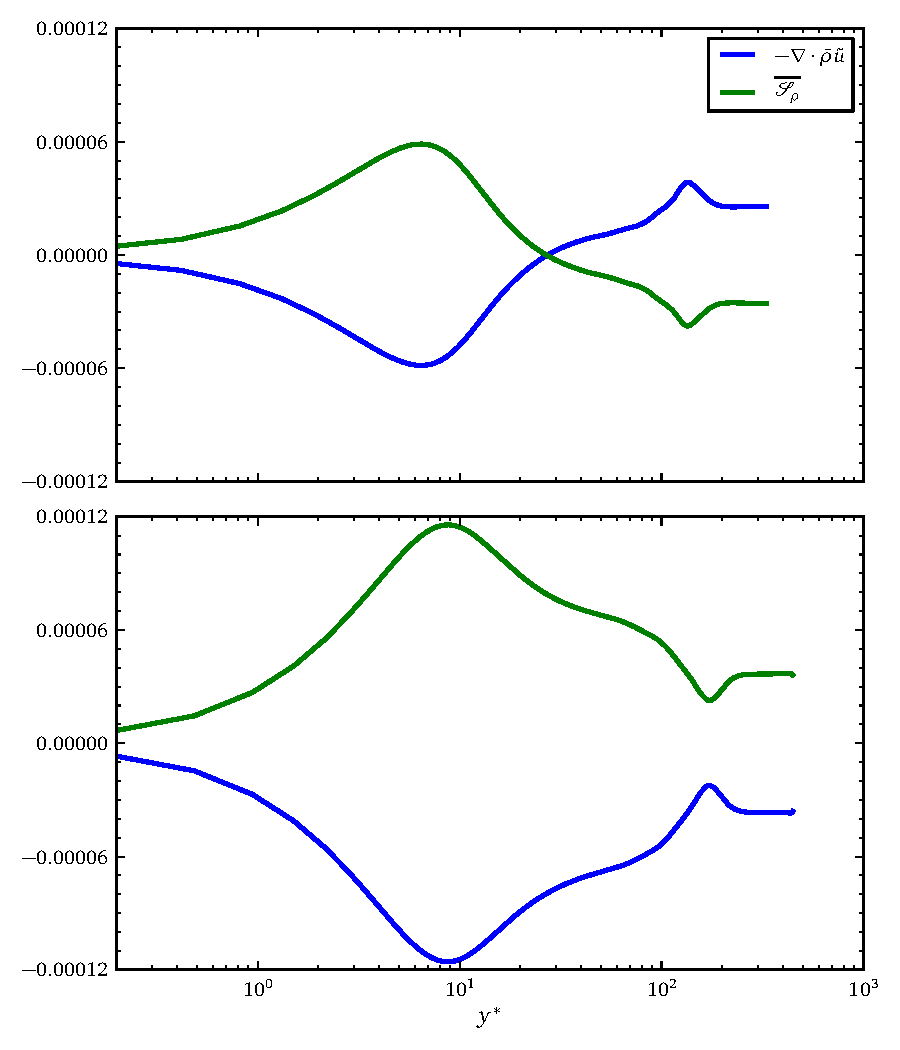
\includegraphics[width=\textwidth]{hqd_fans_rho}
\caption[Density equation budget for simulations t3.199 and t4.134]{%
    Budget for the Favre-averaged density~\eqref{eq:fans_mass}
    in simulations t3.199 (above) and t4.134 (below)
    normalized by $\rho_w u_\tau^2 / \nu_w$.\label{fig:fans_rho}
    % Normalize by \rho_w (\partial_y u)_w
}
\end{figure}

\begin{figure}
\centering
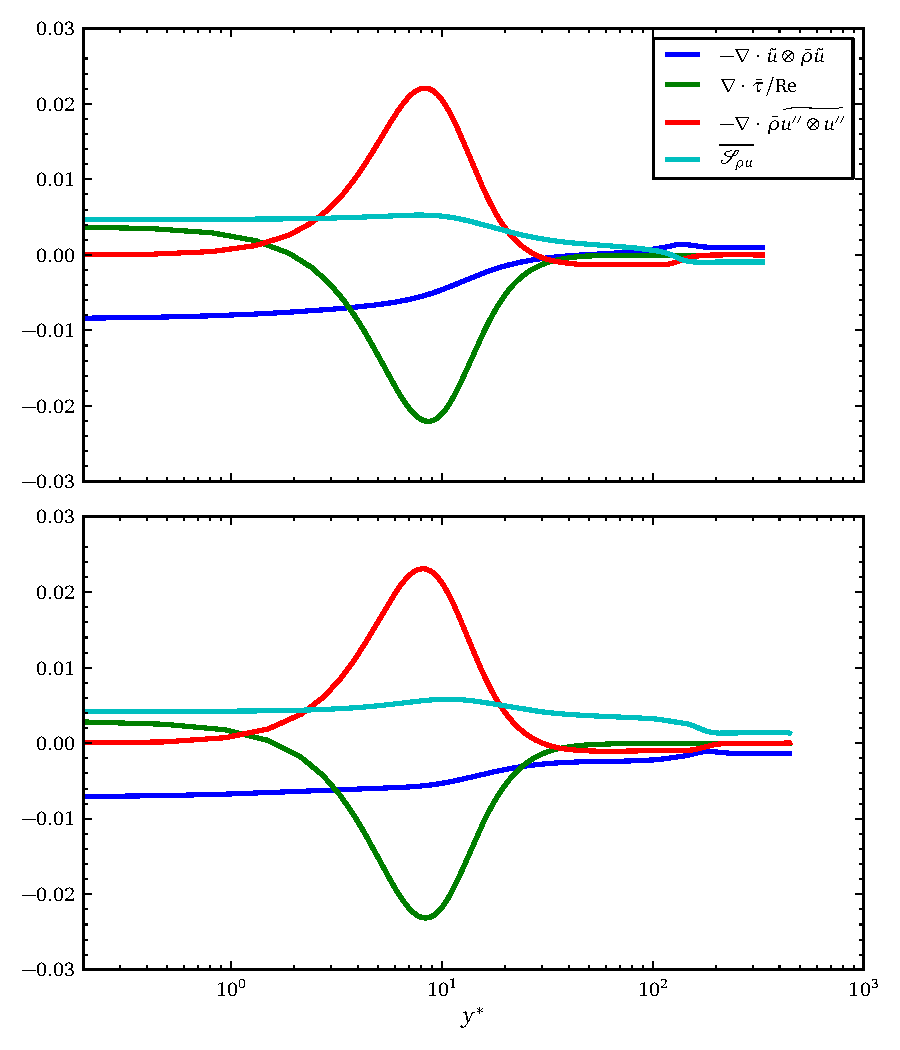
\includegraphics[width=\textwidth]{hqd_fans_rho_u}
\caption[Streamwise momentum equation budget for cases t3.199 and t4.134]{%
    Budget for the Favre-averaged streamwise momentum~\eqref{eq:fans_mom}
    in simulations t3.199 (above) and t4.134 (below)
    normalized by $\rho_w u_\tau^3 / \nu_w$.\label{fig:fans_rho_u}
    % Normalize by \rho_w (\partial_y u)_w u_\tau with u_tau having units u_0
}
\end{figure}

\begin{figure}
\centering
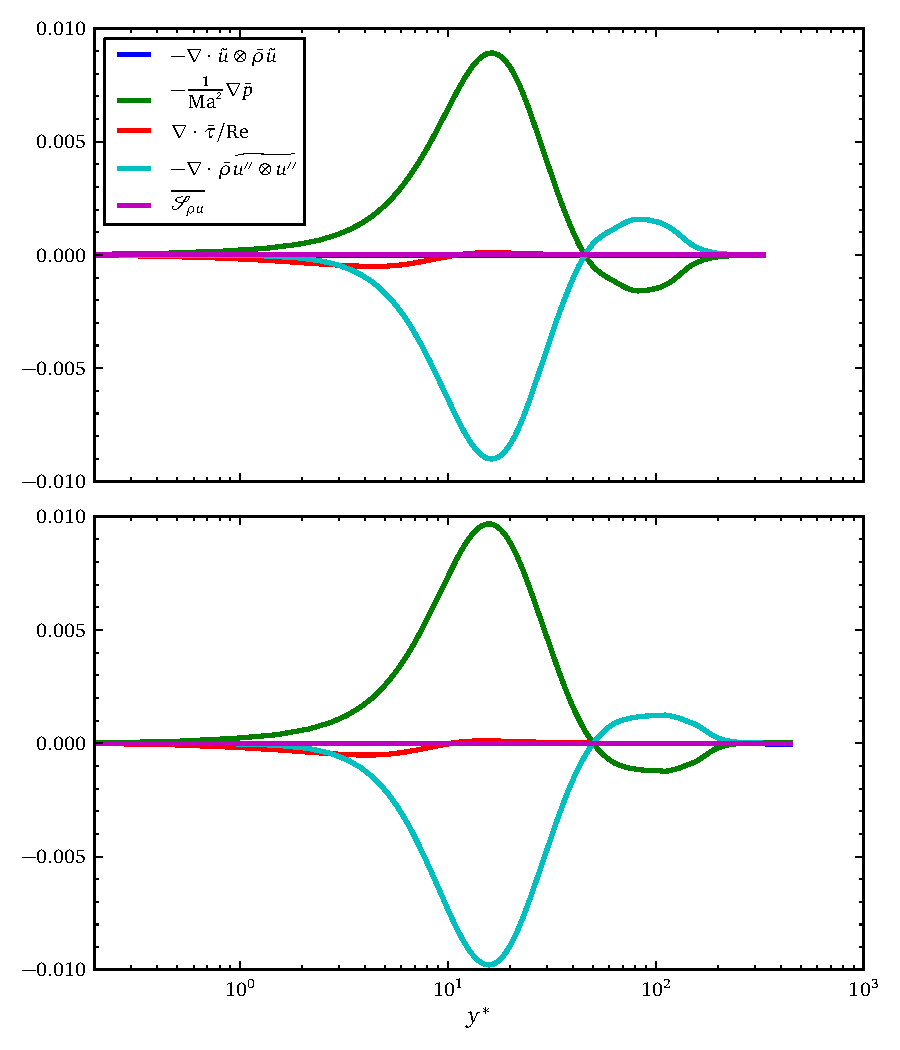
\includegraphics[width=\textwidth]{hqd_fans_rho_v}
\caption[Wall-normal momentum equation budget for cases t3.199 and t4.134]{%
    Budget for the Favre-averaged wall-normal momentum~\eqref{eq:fans_mom}
    in simulations t3.199 (above) and t4.134 (below)
    normalized by $\rho_w u_\tau^3 / \nu_w$.\label{fig:fans_rho_v}
    % Normalize by \rho_w (\partial_y u)_w u_\tau with u_tau having units u_0
}
\end{figure}

%% Spanwise momentum is zero by symmetry so this plot is just statistical noise
%\begin{figure}
%\centering
%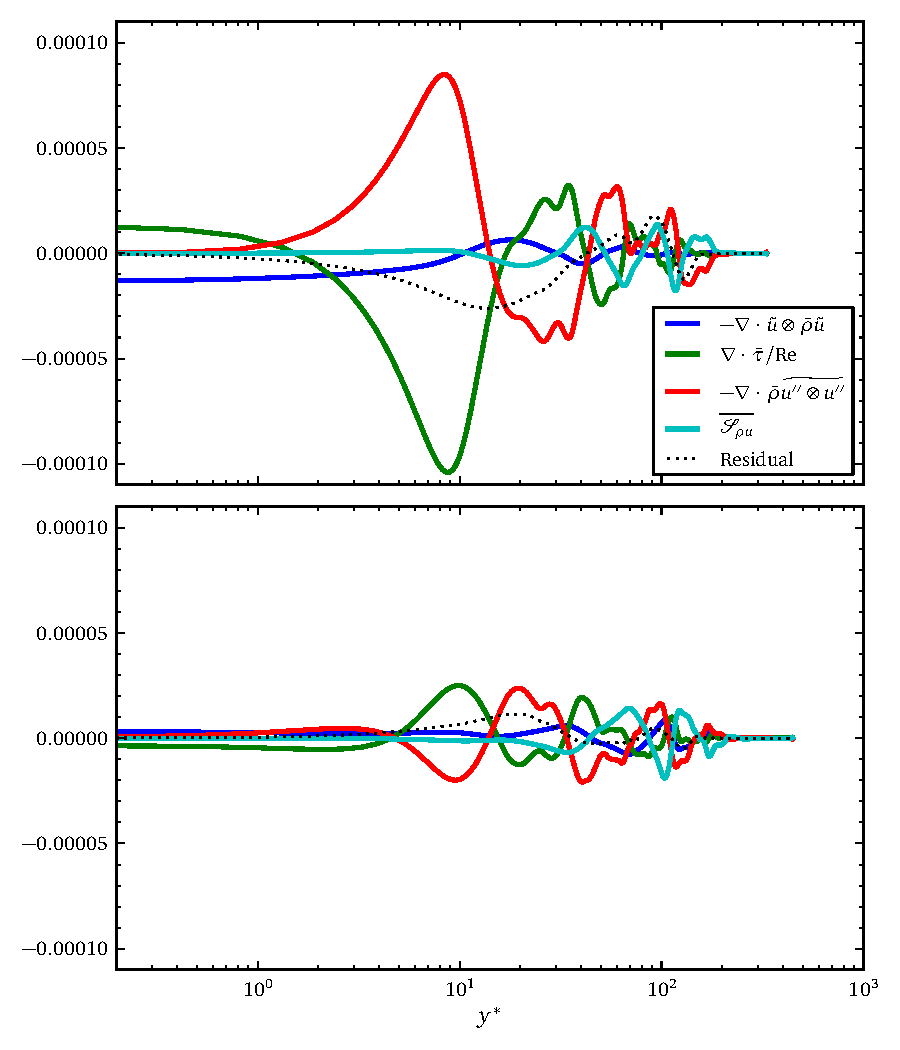
\includegraphics[width=\textwidth]{hqd_fans_rho_w}
%\caption[Spanwise momentum equation budget for cases t3.199 and t4.134]{%
%    Budget for the Favre-averaged spanwise momentum~\eqref{eq:fans_mom}
%    in simulations t3.199 (above) and t4.134 (below)
%    normalized by $\rho_w u_\tau^3 / \nu_w$.\label{fig:fans_rho_w}
%    % Normalize by \rho_w (\partial_y u)_w u_\tau with u_tau having units u_0
%}
%\end{figure}

\begin{figure}
\centering
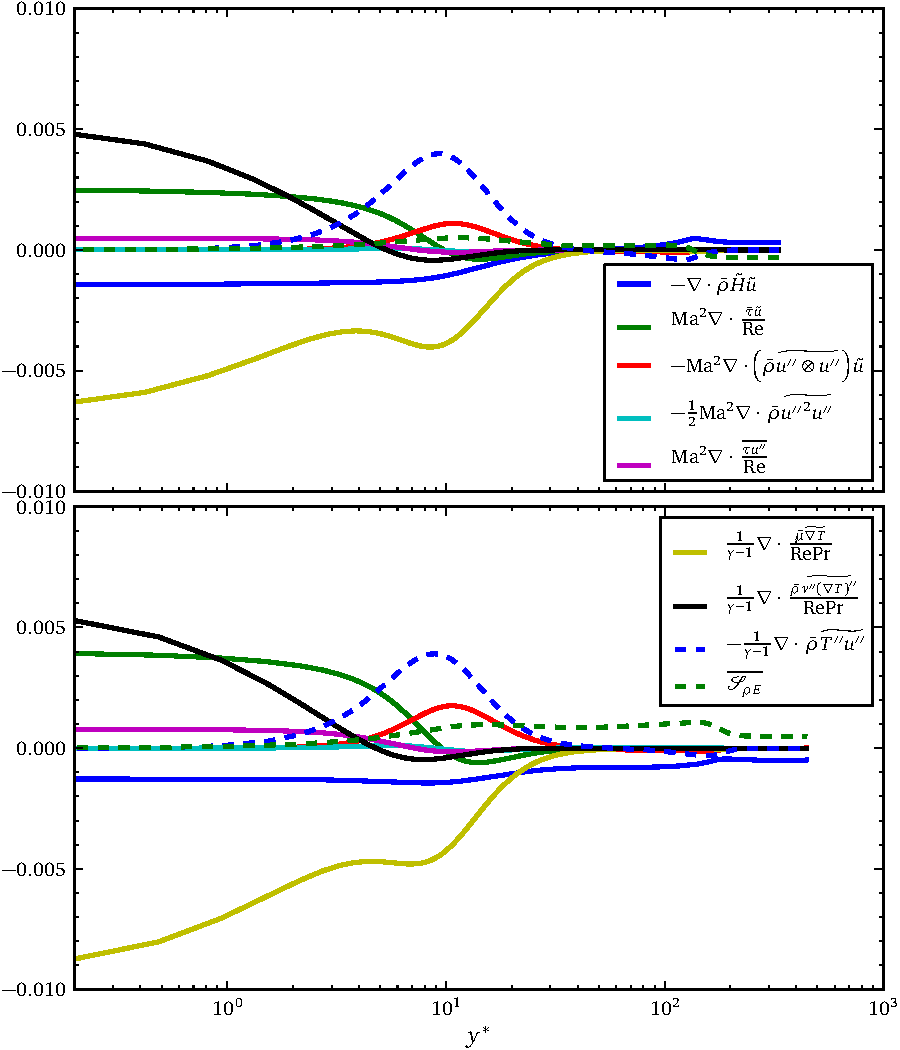
\includegraphics[width=\textwidth]{hqd_fans_rho_E}
\caption[Total energy equation budget for simulations t3.199 and t4.134]{%
    Budget for the Favre-averaged total energy~\eqref{eq:fans_energy}
    in simulations t3.199 (above) and t4.134 (below) normalized by
    $\rho_w a_w^2 u_\tau^2 / \nu_w$.\label{fig:fans_rho_E}
    % Normalize by \rho_w T_w (\partial_y u)_w
}
\end{figure}

\begin{figure}
\centering
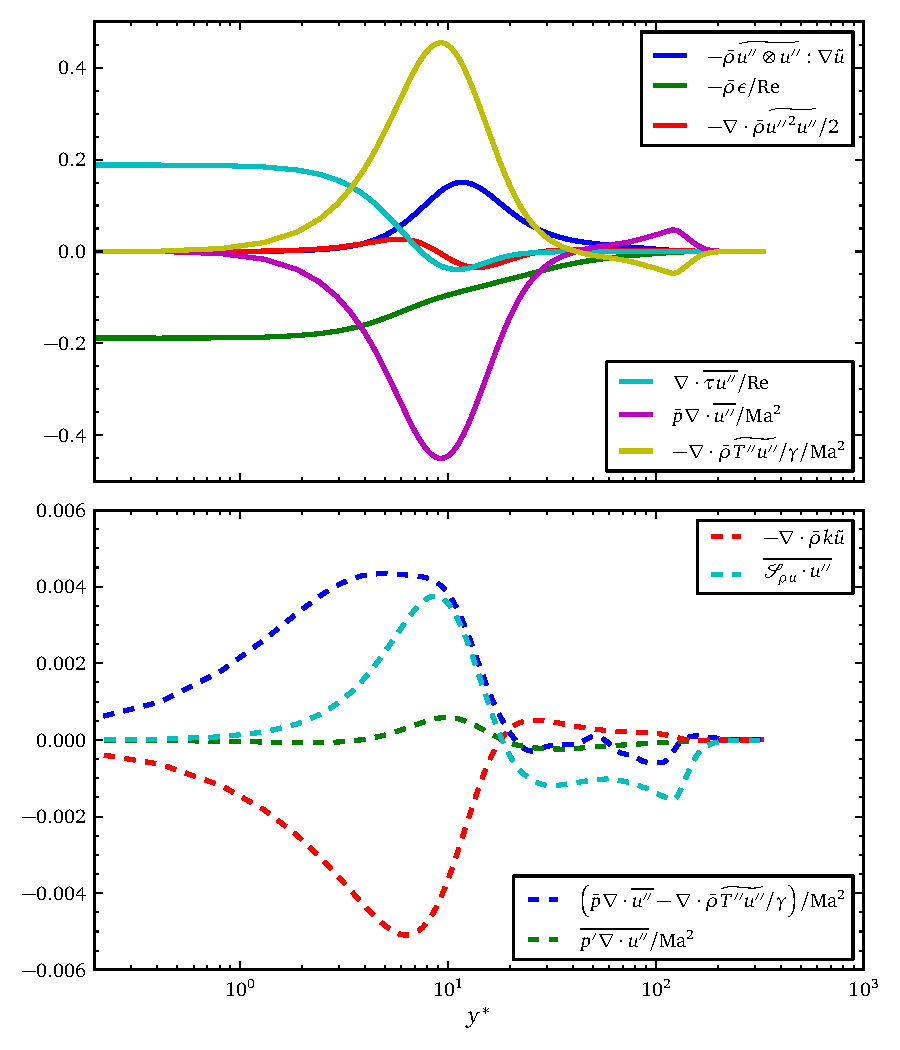
\includegraphics[width=\textwidth]{hqd_tke_t3199}
\caption[Turbulent kinetic energy equation budget for simulation t3.199]{%
    Budget for the turbulent kinetic energy~\eqref{eq:fans_tke} in simulation
    t3.199 normalized by $\rho_w u_\tau^4 / \nu_w$.  More significant terms
    appear in the upper half of the figure while less significant contributions
    appear in the lower half.  Two nearly symmetric thermodynamic terms
    above have their sum duplicated below.\label{fig:tke_t3199}
    % Normalize by \mu_w (\partial_y u)_w^{2} / Re
}
\end{figure}

\begin{figure}
\centering
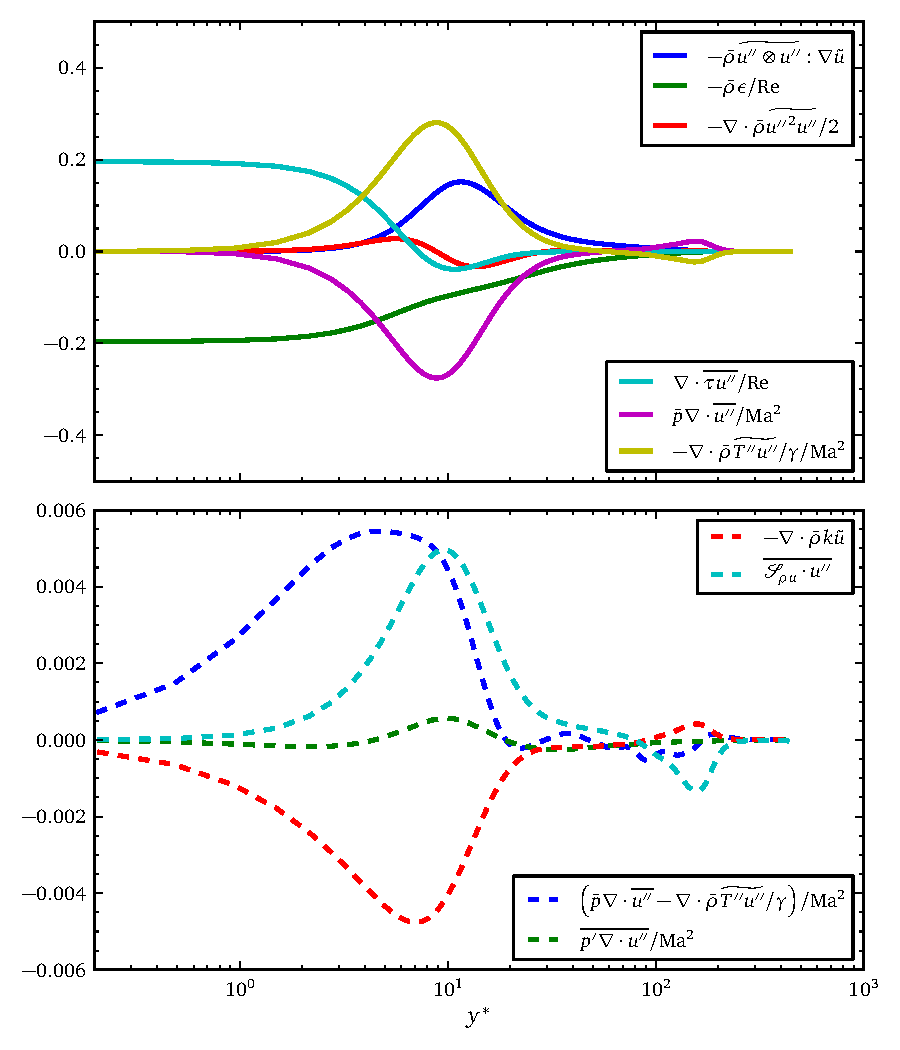
\includegraphics[width=\textwidth]{hqd_tke_t4134}
\caption[Turbulent kinetic energy equation budget for simulation t4.134]{%
    Budget for the turbulent kinetic energy~\eqref{eq:fans_tke} in simulation
    t4.134 normalized by $\rho_w u_\tau^4 / \nu_w$.  More significant terms
    appear in the upper half of the figure while less significant contributions
    appear in the lower half.  Two nearly symmetric thermodynamic terms
    above have their sum duplicated below.\label{fig:tke_t4134}
    % Normalize by \mu_w (\partial_y u)_w^{2} / Re
}
\end{figure}


\chapter[Detecting Turbulence-Sustaining Regions\\ on Blunt-Bodied Reentry Vehicles]
        {Detecting Turbulence-Sustaining Regions on Blunt-Bodied Reentry Vehicles}
\label{sec:relam}

To reduce transition-driven uncertainty in aerothermodynamic heating
predictions, spatiotemporally homogenized direct numerical simulation
(DNS) was used to bound the turbulence-sustaining region on a blunt-bodied reentry
vehicle.  This chapter applies the ideas set forth in
\autoref{sec:detectingrelaminarization} to investigate which regions on the NASA
Orion MPCV thermal protection system cannot sustain turbulence during the peak
heating phase of return from the International Space Station.
%
That particular reentry scenario, described in \autoref{sec:orionmpcv},
was selected because of the availability of simulation data by
\citeauthor{Bauman2011Loose} and because of the upcoming NASA Exploration Flight
Test-1~\citep{SpaceCom20140317}.  Though that test will more closely resemble
the Orion MPCV returning from Earth's moon rather than the International Space
Station, it is nevertheless expected to produce experimental flight data against
which our simulation-based predictions might later be compared.
%
The method is described in \autoref{sec:relam_methods}.  Results and discussion
follow in Sections~\ref{sec:relam_results} and~\ref{sec:relam_discussion}.


%%%%%%%%%%%%%%%%%%%%%%%%%%%%%%%%%%%%%%%%%%%%%%%%%%%%%%%%%%%%%%%%%%%%%%%%%%%%%%
\section{Method}
\label{sec:relam_methods}

The method is broken into three sequential phases.
%
First, local conditions on the Orion MPCV heat shield surface during a fully
laminar reentry are quantified to identify the search space over which the
turbulence-sustaining study will proceed.
%
Second, spatiotemporal DNS are prepared at local conditions representative of
the heat shield edge with the goal of sustaining at least one statistically
stationary turbulent simulation.
%
Third, starting from a stationary simulation, the parameters are
adjusted to incrementally reflect conditions found increasingly closer to the
Orion MPCV stagnation point which are less likely to sustain turbulence.
%
If at this stage the flow relaminarizes, or at least enters a demonstrably
``quasi-laminar'' state~\citep{Sreenivasan1982Laminarescent}, the
turbulence-sustaining region boundary has been detected.
%
These three phases are elaborated in the remainder of this section.

%%%%%%%%%
% PHASE 1
%%%%%%%%%

In the first phase, an assumed laminar flow field over the Orion MPCV thermal
protection system was obtained from a simulation by P. T.
Bauman~\citep{Kirk2014Modeling,Bauman2011Loose}.  The laminar solution captured
the bow shock on the vehicle, accommodated the resulting high temperature
aerothermochemistry, included the curved MPCV geometry as the flow passed over
the thermal protection system, and incorporated a chemically reacting ablator
actively maintaining a cold wall despite the incoming enthalpy flux.  This
solution was post-processed to extract local boundary layer quantities of
interest along the thermal protection system symmetry plane, pictured in
\autoref{fig:cev_symplane}, producing the results already shown in
Figures~\ref{fig:cevisslam_summary1} and~\ref{fig:cevisslam_summary_fpg}.
%
Those quantities are the Reynolds number based on momentum thickness
$\Reynolds[\theta]{}$, the edge Mach number $\Mach[e]{}$, the favorable pressure
gradient strength as measured by the parameter
$p_{e,\xi}^{\ast}$~\eqref{eq:defnpexi}, the wall blowing velocity normalized by
the friction velocity $v_w^{+} = v_w / u_\tau$, the coldness of the wall
relative to the boundary layer edge $T_e/T_w$, the Prandtl number $\Prandtl$,
and the ratio of specific heats $\gamma = C_p / C_v$.
%
Out of the many possible pressure gradient parameters
that the study could target,
$p_{e,\xi}^{\ast}$ was chosen motivated by the needs of the inviscid base flow
design process of Appendix~\ref{sec:radialflow} in conjunction with that
procedures' successful application in \autoref{sec:bldata}.

At each location on the thermal protection system surface the above quantities
collectively characterize the subset of the peak heating boundary layer physics
that can be captured by the governing equations from \autoref{sec:goveqn}.
%
Mapping Bauman's complex, multiphysics solution onto this comparatively simple
Navier--Stokes formulation crudely approximates high temperature reacting air by
a perfect gas.  Further, variations in the Prandtl number and ratio of specific
heats are neglected and replaced by constant air values $\Prandtl=0.7$ and
$\gamma=1.4$.  A power law viscosity was assumed with exponent
$\beta=\nicefrac{2}{3}$ based on fitting high temperature air data as shown in
\autoref{fig:Svehla1962}.
%
At the end of the phase, the entire reentry scenario had been reduced to a
single mapping of the distance leeward from the vehicle's stagnation point
to the five nondimensional local conditions:
$\Reynolds[\theta]{}$, $\Mach[e]{}$, $T_e/T_w$, $v_w^{+}$, and
$p_{e,\xi}^{\ast}$.

\begin{table}[p]
\makecommand{\z}{\phantom{0}}  % Facilitates column alignment
\makecommand{\Z}{\phantom{.0}} % Ditto
\centering
\caption[%
    Selected locations from the fully laminar Orion MPCV TPS simulation
]{%
    Selected reacting boundary layer conditions from the symmetry plane
    on a fully laminar Orion MPCV thermal protection system simulation
    depicted more fully in Figures~\ref{fig:cevisslam_summary1}
    and~\ref{fig:cevisslam_summary_fpg}.  Column ``Location'' indicates
    the number of meters leeward of the stagnation point where the
    conditions are found.\label{tbl:cevisslam_detail1}
}
\begin{tabular}{cccccc}
Location                              &
$\textrm{Re}_{\theta}$                & % Re_theta
$\textrm{Ma}_{e}$                     & % Ma_edge
$T_{e}/T_w$                           & % T_ratio
$v_w^{+}$                             & % v_wallplus
\raisebox{0.10ex}{$p_{e,\xi}^{\ast}$}   % p_exi
\\
\toprule\toprule
%Location  &  Re_theta  &  Ma_edge  &  T_ratio &  v_wallplus  &  p_exi           \\
4.134~m    &  223       &  1.152\z  &  4.285   &  0.007178    &  \num{-0.01235}  \\
3.199~m    &  225       &  0.8986   &  4.262   &  0.008387    &  \num{-0.01019}  \\
2.299~m    &  177       &  0.6597   &  4.182   &  0.009765    &  \num{-0.01269}  \\
1.389~m    &  114       &  0.4112   &  4.129   &  0.01225\z   &  \num{-0.01793}
\end{tabular}
\end{table}

%%%%%%%%%%%%%%%%%%%%%%%%%%%%%%%%%%%%%%%%%%%%%%%%%%%%%%%%%%%%%%%%%%%%%%%%%%%%%%
%%%%%%%%%%%%%%%%%%%%%%%%%%%%%%%%%%%%%%%%%%%%%%%%%%%%%%%%%%%%%%%%%%%%%%%%%%%%%%

\begin{table}
\makecommand{\z}{\phantom{0}}  % Facilitates column alignment
\makecommand{\Z}{\phantom{.0}} % Ditto
\centering
\caption[%
    Input parameters used in the relaminarization study to obtain Orion
    MPCV-like boundary layer conditions
]{%
    Suzerain v0.1.6.34-r45407 input parameters found to approximately
    match local boundary layer conditions at locations in
    \autoref{tbl:cevisslam_detail1}.
    %
    For all cases, $\textrm{Pr} = \mu C_p / \kappa = 0.7$, $\alpha=0$ in
    $\mu_B=\alpha\mu$, $\beta=\nicefrac{2}{3}$ in $\mu / \mu_0={\left(T /
    T_0\right)}^\beta$, and $\gamma = C_p / C_v = 1.4$.
    %
    Extents were $L_x/l_0=10$, $L_y/l_0=2.5$, $L_z/l_0=3$ employing a
    piecewise-quintic B-spline basis with $N_y=192$ collocation points.
    %
    Column ``Advance'' reports which linear implicit operator and
    time step safety factor governed time advance.
    %
    Refer to Tables~\ref{tbl:table_turb_hbl}
    through~\ref{tbl:table_turb_hbl_fpg} for other column
    definitions.\label{tbl:cevisslam_inputs}
}
{\renewcommand{\tabcolsep}{0.345em}
\begin{tabular}{cccccccccc}
Location                                        &%  Location
$\textrm{Re}$                                   &%  Re
$\textrm{Ma}$                                   &%  Ma
$\tanh$                                         &%  tanh
$\operatorname{gr}_{t_0}\!\left(\Delta\right)$  &%  grdelta
$T_w/T_0$                                       &%  Tw
$v_w/u_0$                                       &%  vw
\raisebox{0.10ex}{$p_{e,\xi}^{\ast}$}           &%  p_ex
\multicolumn{2}{c}{Advance}                      %  implicit,safetyfactor
\\
\toprule\toprule
% DATA DRAWN FROM CASES relam${CASE}/last/restart00000.h5
%Location &  Re     &  Ma       &  tanh  &  grdelta    &  Tw      &  vw             &  p_ex            &  implicit  &  safetyfactor  \\
4.134~m   &  1535   &  1.152\z  &  2.2   &  0.02175    &  0.2333  &  \num{1.99e-4}  &  \num{-0.01234}  &  Y         &  0.35\z        \\
3.199~m   &  1475   &  0.8985   &  2.2   &  0.016\z\z  &  0.2346  &  \num{2.20e-4}  &  \num{-0.01019}  &  XYZ       &  0.2\z\z       \\
2.299~m   &  1100   &  0.6598   &  2.0   &  0.01\z\z\z &  0.2391  &  \num{2.68e-4}  &  \num{-0.01269}  &  XYZ       &  0.2\z\z       \\
1.389~m   &  \z800  &  0.4113   &  2.0   &  0.0035\z   &  0.2422  &  \num{3.68e-4}  &  \num{-0.01793}  &  XYZ       &  0.175
\end{tabular}}
\end{table}


%%%%%%%%%
% PHASE 2
%%%%%%%%%

In the second phase, the direct numerical simulation code Suzerain was used to
prepare spatiotemporally homogenized flow fields at several ``locations'' from
the reentry-specific mapping described above.  Only one
location at the heat shield edge was required to proceed to the third phase.
%
However, as multiple independent locations easily could be made ready
simultaneously, four locations roughly quadrisecting the search space were
prepared.

\autoref{tbl:cevisslam_detail1} documents the four selected locations.
%
Locations 3.199~m and 4.134~m correspond to $\Reynolds[\theta]{}=223$ and
$225$ variants of the scenario conditions found in \autoref{sec:bldata}
simulations t3.199 and t4.134, respectively.
%
Both of these locations were expected to sustain turbulence based on the
\citet[\textsection{}3.2]{Spalart1988Direct} finding that his constant
viscosity, homogenized sink flow simulations quickly relaminarized below
$\Reynolds[\theta]{}=330$ because 3.199~m and 4.134~m have appreciably higher
momentum Reynolds numbers when evaluated using wall viscosity
(\autoref{fig:cevisslam_summary1}).
%
Having cases at subsonic and supersonic conditions was done to hedge against the
possibility of either the spatiotemporal homogenization or the inviscid base
flow design procedure becoming numerically problematic if the third phase of
this study dictated iteratively adjusting a simulation across
$\Mach[e]{}=1$.\footnote{%
    Concern about the spatiotemporal homogenization in supersonic circumstances
    arose based on observations reported at the end of
    \autoref{sec:bldata_stats}.  Concerns about the base flow procedure stemmed
    from the design procedure of Appendix~\ref{sec:radialflow_match} driving the
    nozzle radius $R$ to large values as $\Mach[e]$ approaches one from either
    direction.
}
%
Either location 2.299~m or 1.389~m was hypothesized to relaminarize.

At each of those four locations the MPCV-derived data in
\autoref{tbl:cevisslam_detail1} furnished fixed values for only
the Suzerain code input parameters $\Mach\approx{} u_{99} /
a_{99}$, $T_w/T_0$, and $p_{e,\xi}^{\ast}$.
%
As doing so had proved successful for \autoref{sec:bldata},
boundary layer thickness $\delta_{99}/l_0=1$ was chosen as a
target to be achieved indirectly by adjusting the slow growth rate
$\operatorname{gr}_{t_0}\!\left(\Delta\right)$.
%
When that condition is met, the nondimensional formulation in conjunction with
the inviscid base flow design procedure \emph{a priori} causes $\rho_{99} /
\rho_0$, $u_{99} / u_0$, and $T_{99} / T_0$ to all be nearly one.
%
Appropriate values for the remaining code inputs $\Reynolds\approx \rho_{99}
u_{99} \delta_{99} / \mu_{99}$, $\operatorname{gr}_{t_0}\!\left(\Delta\right)$,
and $v_w/v_0$ had to be discovered.
%
An elegant way to discover suitable settings would be to invert for the
appropriate values using a spatiotemporally equipped turbulence model
implementation properly calibrated for the current context.
%
A less elegant way would be to iteratively seek values with such a tool in lieu
of the more complicated inversion procedure.
%
The inelegant way used in this study was to perform exploratory simulations to
manually acquire the needed values by iteratively adjusting code input
parameters until the desired stationary behavior was obtained.
%
\autoref{tbl:cevisslam_inputs} reports those parameters.
%
To conserve compute resources, these computations used coarse streamwise and
spanwise resolution (for example, $\Delta{}x^{+}\approx{}30$) but production
wall-normal bases with $y^{+}_1$ and $y^{+}_{10}$ comparable or better than
those in \autoref{tbl:table_turb_hbl}.
%
Final tests to ensure the parameters appearing in \autoref{tbl:cevisslam_inputs}
were robust on near-production grids (for example, $\Delta{}x^{+}\leq{}25$ and
$\Delta{}z^{+}\leq{}15$) yielded unexpected results which will be conveyed in
\autoref{sec:relam_results_refine}.

%%%%%%%%%
% PHASE 3
%%%%%%%%%


For the third phase, the code input parameters shown in
\autoref{tbl:cevisslam_inputs} were used to adjust a fully turbulent field so
it matched the target conditions derived from MPCV data.
%
A known-good turbulence field was required to ensure that the relaminarization
study was seeded with a reasonable approximation of boundary layer physics.
Moreover, turbulent conditions are a ``large perturbation'' with respect
to a relaminarized flow per the energy method ideas discussed in
\autoref{sec:energyperturbationtheory}.
%
That adjustment process
is simpler if the initial field already resembles the target flow conditions.
Simulations t3.199 and t4.134 from \autoref{sec:bldata} were designed to serve
exactly that purpose.  They differed from \autoref{tbl:cevisslam_detail1} locations 3.199~m and 4.134~m only in
their $\Reynolds[\theta]{}$ magnitudes.
%
Results starting from these initial conditions will appear in
\autoref{sec:relam_results_turb}.

Though the collapse of turbulent fluctuations and relaminarization can be a
quick process in spatially evolving boundary layers subjected to pressure
gradients~\citep{Mukund2006Relaminarization} and spatially homogenized boundary
layers~\citep[\textsection{}3.2]{Spalart1988Direct}, it was uncertain if that
would also be true for the \citet{Topalian2014Spatiotemporal} spatiotemporal
homogenization or if this slow growth formulation would bring about an
extended ``quasi-laminar'' state~\citep{Narasimha1979Relaminarization,
Sreenivasan1982Laminarescent} that would prove difficult to identify.  An
extended relaminarization process would retard our ability to incrementally move
to locations nearer the stagnation point because it would force us to simulate
each station for a longer duration to ensure we did not accidentally pass over
the critical location.
%
For this reason, an \emph{in situ} capability to assess the strength of the
turbulence by monitoring the temporal trace of relevant quantities was added to
Suzerain.  Following findings by \citet{Cal2008Similarity}, the code was
augmented to frequently output maxima values and locations for absolute values
of Reynolds-averaged and Favre-averaged stress tensor components.  Output of the
wall-normal location and value of the peak streamwise- and spanwise-averaged
production term as well as its integrated magnitude was also added.  These
monitors permitted early identification of relaminarization precursors.

An insufficiently large computational domain and inadequate spatial resolution
tend to cause turbulent fluctuations to persist.  The former introduces
artificially long correlation lengths and the latter does not permit turbulent
kinetic energy to be dissipated properly.  Either effect would likely cause the
study to incorrectly detect the turbulence-sustaining region.  Plans were laid
to repeat the final stages of the detection process with a larger domain and
improved resolution.

%An early draft:
%\begin{enumerate}
%\item Given scenario parameters/base flows, compute stationary 1D laminar
%profiles at each location on the CEV.  These local heat flux at the wall
%magnitudes serve as canaries for when relaminarization is occurring.
%Initially, we say the flow has relaminarized if a turbulent case's heat flux at
%the wall is within 10\% of these local laminar results.
%\item Choose a location A possessing the maximal $\Reynolds[\delta^\ast]$ among
%all locations.  Initialize a small box simulation at reasonable resolution (per
%Victor/Wu) for A's base flow.  Run until stationary.  If not stationary, freak
%out.
%\item Choose a location B a small distance from the stagnation point where
%turbulence is not expected.  Take stationary field from A and instantaneously
%adjust scenario parameters to match location B.  Run B until it relaminarizes
%noting the amount of simulation time necessary to achieve that decay as
%measured relative to wall heat flux to laminar wall heat flux ratio.  If B does
%not relaminarize or takes too long, freak out.
%\item Partition A to B into O(10) segments [A0, A1), [A1, A2), ..., [A8, A9)
%where A0 = A, A9 = B.
%\item Set i = 0.
%\item Take stationary field from A(i-1) and instantaneously adjust to match
%conditions at A(i).  Run simulation.
%\begin{enumerate}
%    \item If A9 = B reached and flow hasn't relaminarized, freak out.
%    \item If run becomes stationary, i+=1 and repeat 6.
%    \item If run relaminarizes, [A(i-1), A(i)) likely contains the
%    relaminarizing cusp.  Continue.
%\end{enumerate}
%\item Partition A(i-1) to A(i) into O(10) segments and repeat steps 6 and 7 on
%this finer gradation.
%\item Presumably now, for the chosen box and grid, we know exactly where the
%behavioral cusp is.
%\item Initialize a new small box run at A on a finer resolution.  Quickly move
%to confirm behavioral cusp with finer resolution.
%\item Initialize a new big box run at modest resolution.  Quickly move to
%confirm behavioral cusp with larger box size.
%\item If no cause for freaking out, declare success.
%\end{enumerate}
%
%What actually happened:
%\begin{enumerate}
%\item Took turbulent fields from prior chapter, coarsened, and aimed for
%    conditions 1.389, 2.299, 3.199, and 4.134 meters leeward of the stagnation
%    point.
%\begin{enumerate}
%    \item Location 1.389 promptly relaminarized
%    \item Location 2.299 relaminarized
%    \item Location 3.199 relaminarized with a small dwell
%    \item Location 4.134 relaminarized over a timeframe of nearly 9 turnovers
%    \item STARTHERE
%\end{enumerate}
%
%\end{enumerate}

%%%%%%%%%%%%%%%%%%%%%%%%%%%%%%%%%%%%%%%%%%%%%%%%%%%%%%%%%%%%%%%%%%%%%%%%%%%%%%
\section{Results}
\label{sec:relam_results}

Two distinct sets of results are presented.
%
The first set of results, found in \autoref{sec:relam_results_refine}, conveys
the unexpected behavior observed when coarse, fluctuation-sustaining exploratory
simulations were refined to production resolutions.
%
The second set of results, appearing in \autoref{sec:relam_results_turb},
investigates relaminarization using fully turbulent fields from
\autoref{sec:bldata} so that the initial conditions represent boundary layers
like those found on the Orion MPCV.


%%%%%%%%%%%%%%%%%%%%%%%%%%%%%%%%%%%%%%%%%%%%%%%%%%%%%%%%%%%%%%%%%%%%%%%%%%%%%%
\subsection{Results from Refining Coarse Exploratory Simulations}
\label{sec:relam_results_refine}

All four coarse simulations performed to discover inputs for
\autoref{tbl:cevisslam_inputs} relaminarized when refined to
$\Delta{}x^{+}\leq{}25$ and $\Delta{}z^{+}\leq{}15$.  The relaminarization
events were not cleanly captured--- initially they were thought to be merely
undesirable drift relative to target conditions which prompted us to adjust code
inputs partway through each event.  After appreciating what had occurred, the
process was repeated but, unlike before, without any adjustments to code inputs
once the simulations were underway.

Figure~\vref{fig:relam4134} shows the temporal evolution of the supersonic coarse
location 4.134~m simulation immediately after refinement.  The earliest time
shown is when the field was refined to $\Delta{}x^{+}\approx{}18.7$ and
$\Delta{}z^{+}\approx{}11.2$ ($N_x = 256$ and $N_z=128$) while holding the
wall-normal basis constant.  As the projection onto a larger Fourier basis is an
exact operation, the refinement does not perturb the flow but it does permit the
solution to populate higher wavenumbers and thereby gain additional dissipative
capability.  The upper six subplots in \autoref{fig:relam4134} show the desired
location-specific conditions as a horizontal dashed line and the actual
simulation evolution in blue curves.
%
The mean flow in the freestream approximately traverses the streamwise extent of
the domain once every 10 time units because because $u_{99}/u_0\approx{}1$ and
$L_x/l_0=10$.
%
For example, $\Reynolds[\theta]$ starts
out slightly too high, grows slowly until just before nondimensional time index 120,
and then gradually drops.  Proceeding down the subplots, the edge Mach number
is seen to be very close to target while the temperature ratio is low.  Wall
blowing $v_w^{+}$, the pressure gradient parameter $p_{e,\xi}^\ast$, and the
boundary layer thickness all match the desired values.

The lower three
subplots in \autoref{fig:relam4134} show turbulence diagnostics.
%
The uppermost of the three is the instantaneous mean turbulent production $-
\bar{\rho} \widetilde{u''\otimes{}u''} : \nabla\tilde{u}$ averaged across all
spatial directions.  It is nondimensionalized by edge state similarly to
$\Reynolds$ and $\Mach$ defined earlier.  Production begins to drop
around time 100.  The next subplot down is the pointwise maximum absolute values
of each component of the Favre-averaged stress tensor.
%
To permit visualizing both early- and late-time behavior, the logarithm of the
absolute values are plotted.   The data is clipped below $10^{-8}$ which only
obscures low magnitude information at late times ($t>240$).
%
After $t>120$ the fluctuation magnitudes slowly drop because of the
extra dissipation available due to the increased spatial
resolution.  As \citet{Cal2008Similarity} reported, the $vv$ and $uv$ curves
decay sharply after the integrated production tails off at $t=180$.  The final
curve is the skin friction factor which decays to a nearly constant value by
$t>300$.
%
Basing $\delta_{99}$ and $u_\tau$ determinations on the initial boundary layer
character, it took roughly 4.2 eddy turnovers\footnote{Computed from $(t_f - t_i) u_\tau / \delta_{99}$.}
from the start of the study until relaminarization precursors appear
and another 1.8 turnovers to reach $t=180$ where the flow
clearly is relaminarizing.

\autoref{fig:relam3199} shows the temporal evolution of the
coarse location 3.199~m simulation immediately after refinement to
$\Delta{}x^{+}\approx{}18.0$ and $\Delta{}z^{+}\approx{}10.8$ ($N_x = 256$
and $N_z=128$).  The $\Reynolds[\theta]$ dips below target, the
$T_e/T_w$ is again low, but the other indirectly controlled parameters
in the upper six subplots
oscillate about the desired values.  Turning to the lower turbulence diagnostics, the
integrated production is quite variable and shows intermittent periods
of decreased production.  The maximum density-weighted stress tensor
components show several relaminarization precursor signatures with the
most pronounced at $t=400$, $t=800$, and $t=1100$.  These are also
seen in the integrated production and skin friction traces.  At each of
those times, however, the fluctuations again kick up and the flow briefly
appears turbulent from these plots.  The dwell time between them is
10.2 and 8.7 eddy turnovers which is longer than the O(6.5) turnover
statistical ensembles gathered in \autoref{sec:bldata}.
%
These three diagnostic subplots show evidence of a characteristic frequency
which may be related to the time scale of the structural interactions
responsible for reinvigorating the fluctuations after each window of decay.
%
From initialization until relaminarization,
36.3 eddy turnovers passed.

\autoref{fig:relam2299} shows the evolution of the coarse location 2.299~m
simulation after refinement to $\Delta{}x^{+}\approx{}14.1$ and
$\Delta{}z^{+}\approx{}8.5$ ($N_x = 256$ and $N_z=128$).  The flow does not
relaminarize over the 23.2 turnovers shown though short lulls appear in the
production during which the stress tensor component magnitudes smooth out due
to dissipation and the skin friction decreases.  Glancing at the top portion of
the figure, however, reveals that wall blowing is too weak and the favorable
pressure gradient too strong on account of the growth rate parameter not
achieving $\delta_{99}\approx{}1$.

\autoref{fig:redux2299} rectifies the target condition mismatch by proceeding
with the new input parameters documented in the figure caption.
Those new parameters took three attempts to discover.
The $T_e/T_w$
target is still too low and the wall blowing just slightly too high, but
overall the disagreement with all target conditions, in particular
the pressure gradient, was remedied.  The production, stress tensor components,
and skin friction continue to show intermittency but location 2.299~m sustained
turbulence for another 23.4 turnovers.  It was unclear whether or not
the intermittency would continue indefinitely or if, eventually,
2.299~m would abruptly collapse as did 3.199~m in \autoref{fig:relam3199}.

Either way, the behavior at 2.199~m appears stationary enough to merit
characterizing the flow.  Based on an ensemble over the data appearing in
\autoref{fig:redux2299}, one-dimensional Fourier spectra were computed and are
presented in \autoref{fig:autocorr-redux2299}.  Comparing against
\autoref{fig:spectra-t3199}, the spectra appear reasonable demonstrating that
the resolution is adequate.  Turning to the two-point correlations, shown in
\autoref{fig:spectra-redux2299},
the appearance of appreciable autocorrelation at length scales on the order of the
approximately $10\delta_{99}\times2.5\delta_{99}\times3\delta_{99}$
domain extent
indicates the finite domain size chosen strongly influences this simulation.
%
Long correlations of this sort are not characteristic of fully developed
turbulence, see \autoref{fig:autocorr-t3199}, suggesting the flow structures are
transitional or marginally turbulent in nature.
%
Due to these
considerable numerical artifacts, the refinement-generated flow targeting
2.299~m conditions that is shown in Figures~\ref{fig:relam2299}
and~\ref{fig:redux2299} does not merit further study as an approximation of a turbulent boundary layer.  However,
this boundary-layer-like flow is interesting as an example of a
self-sustaining, pathologically large perturbation per ideas discussed in
\autoref{sec:energyperturbationtheory}.

Continuing onward with \autoref{fig:relam1389}, location 1.389~m evolution is
pictured after refinement to $\Delta{}x^{+}\approx{}11.7$ and
$\Delta{}z^{+}\approx{}7.0$ ($N_x = 256$ and $N_z=128$).  The simulation
relaminarizes in under 3.6 turnovers.  The lack of a longer ``turbulent dwell''
before relaminarization is thought due to the 1.389~m conditions being unable to sustain
turbulence, rather than an artifact of the initial
field because the long dwell times at 3.199~m and 2.299~m were initialized
in a similar manner.

\begin{figure}
\centering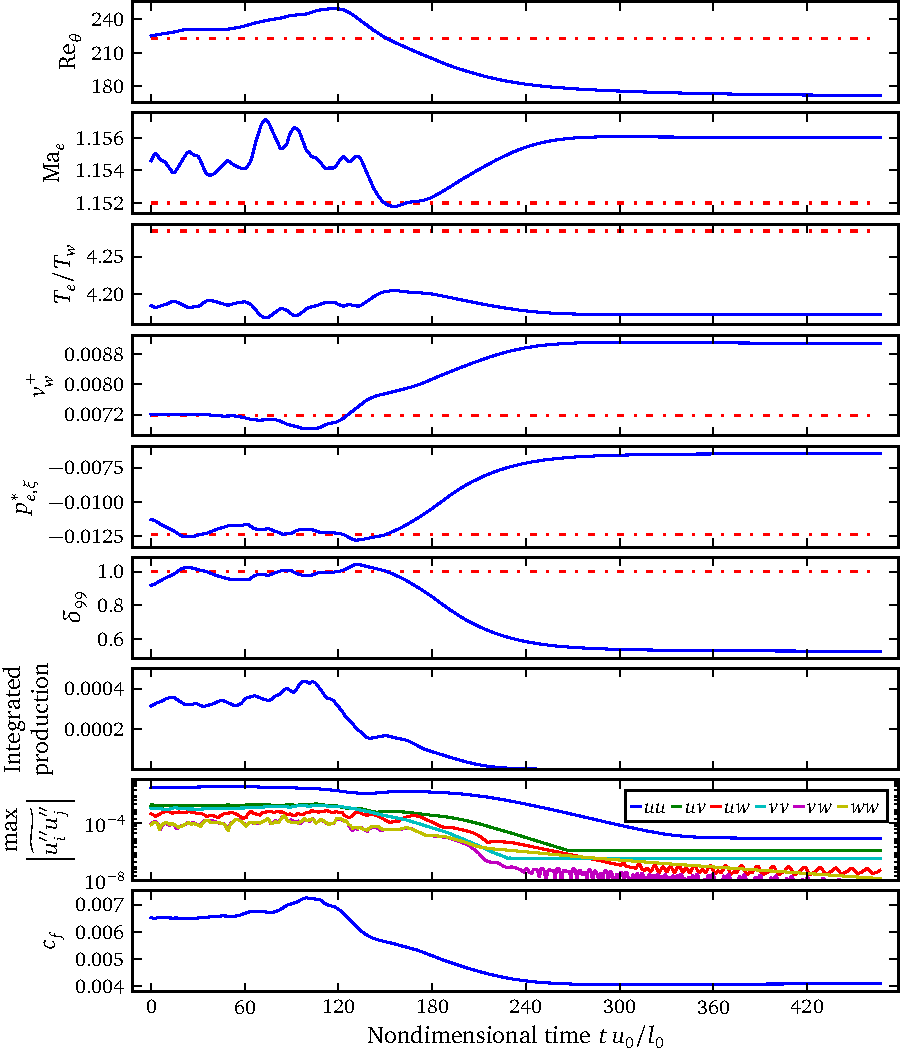
\includegraphics[width=\textwidth]{relam4134}
\caption[Refinement of coarse exploratory simulation for location 4.134~m]{%
    Refinement of exploratory simulation at location 4.134~m.\label{fig:relam4134}
    Dashes mark target conditions.
}
\end{figure}

\begin{figure}
\centering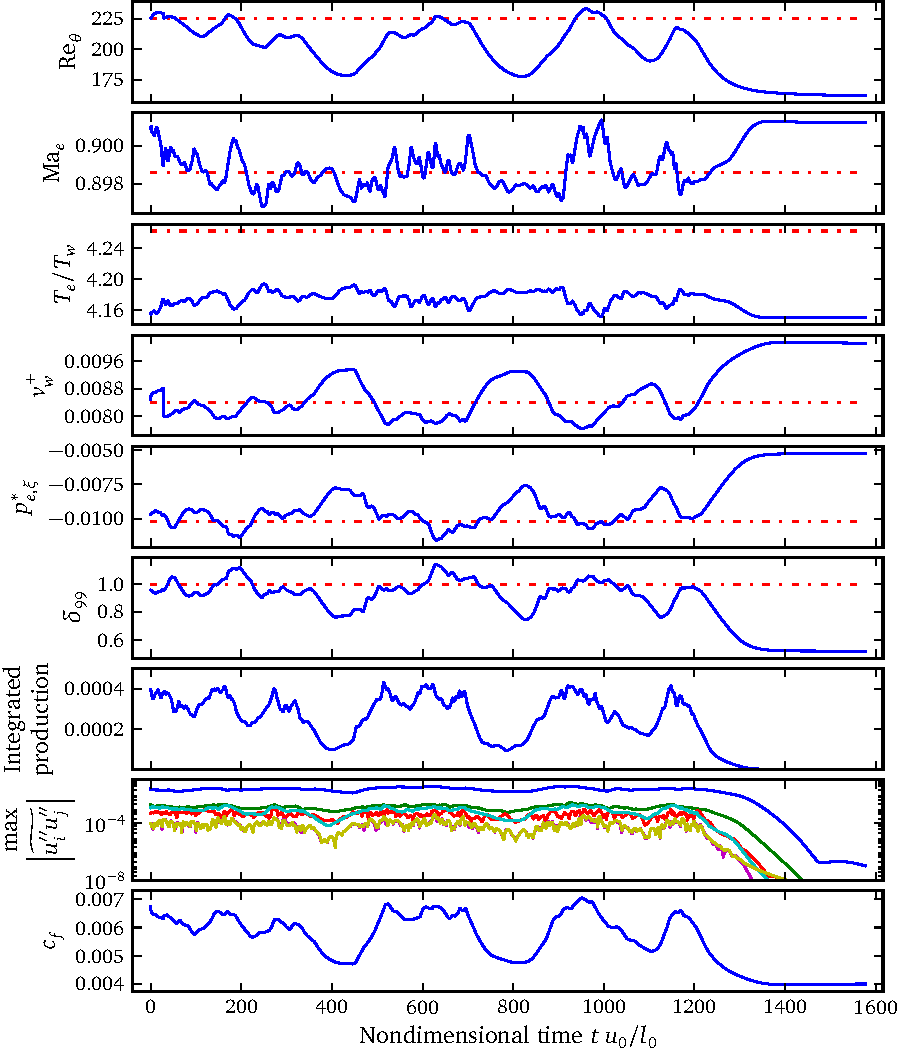
\includegraphics[width=\textwidth]{relam3199}
\caption{Refinement of exploratory simulation for location 3.199~m.\label{fig:relam3199}}
\end{figure}

\begin{figure}
\centering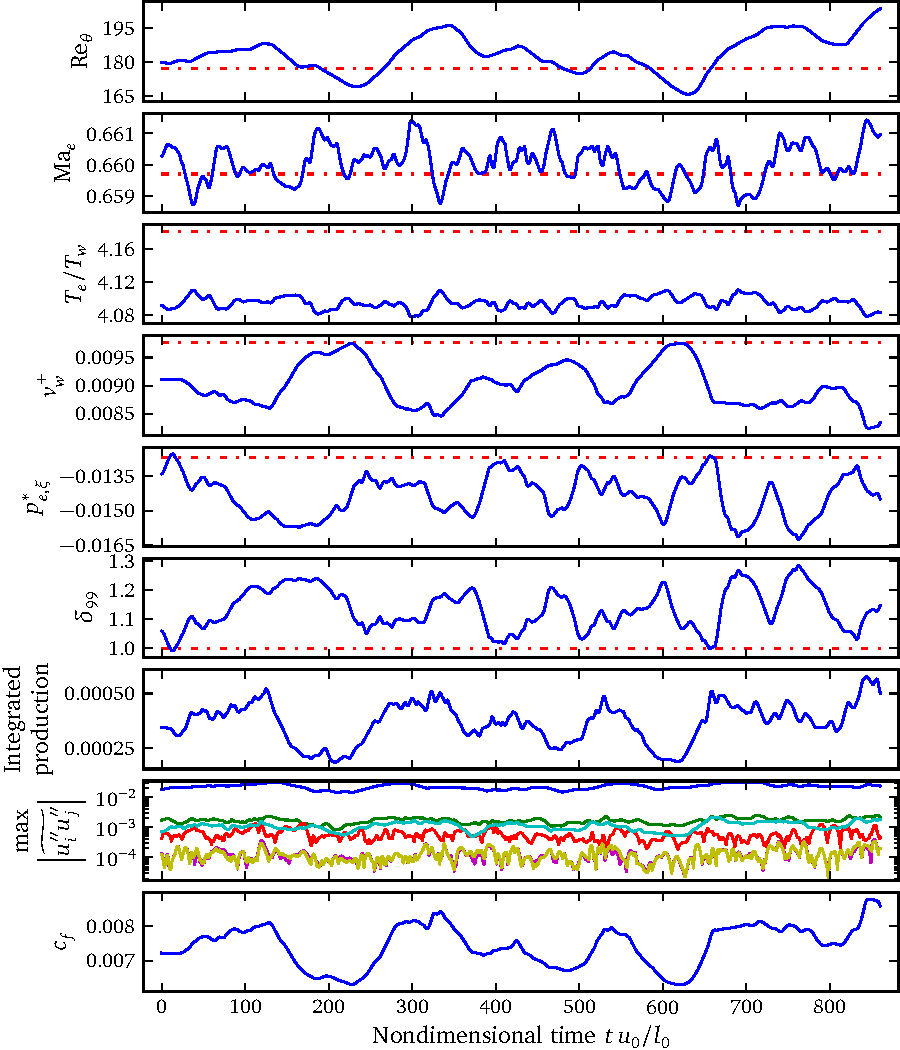
\includegraphics[width=\textwidth]{relam2299}
\caption{Refinement of exploratory simulation for location 2.299~m.\label{fig:relam2299}}
\end{figure}

\begin{figure}
\centering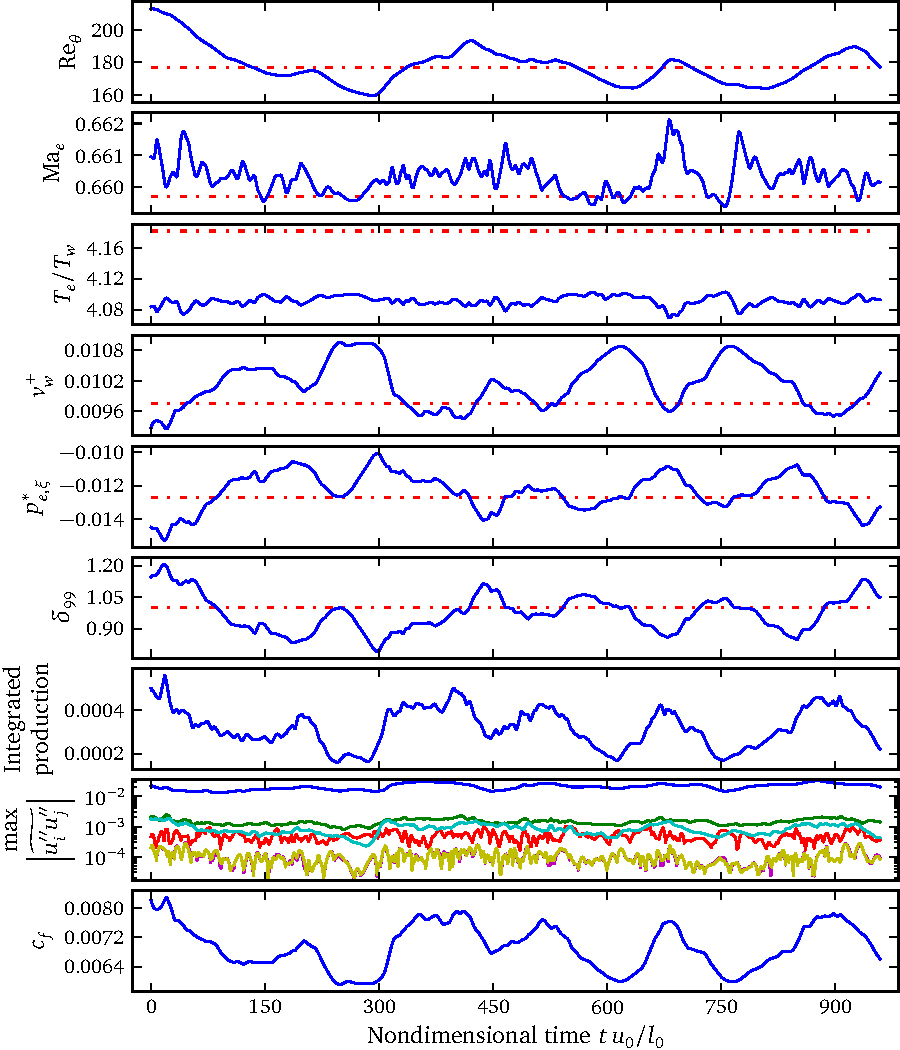
\includegraphics[width=\textwidth]{redux2299}
\caption[Continuation of refinement study for location 2.299~m.]
        {Continuation of refinement study for location 2.299~m.
         Input parameters adjusted to $\Reynolds=1150$,
         $\operatorname{gr}_{t_0}\!\left(\Delta\right)=0.01125$,
         and $v_w/v_0=\num{2.915e-4}$ to better achieve target
         conditions.\label{fig:redux2299}}
\end{figure}


\begin{figure}
\centering
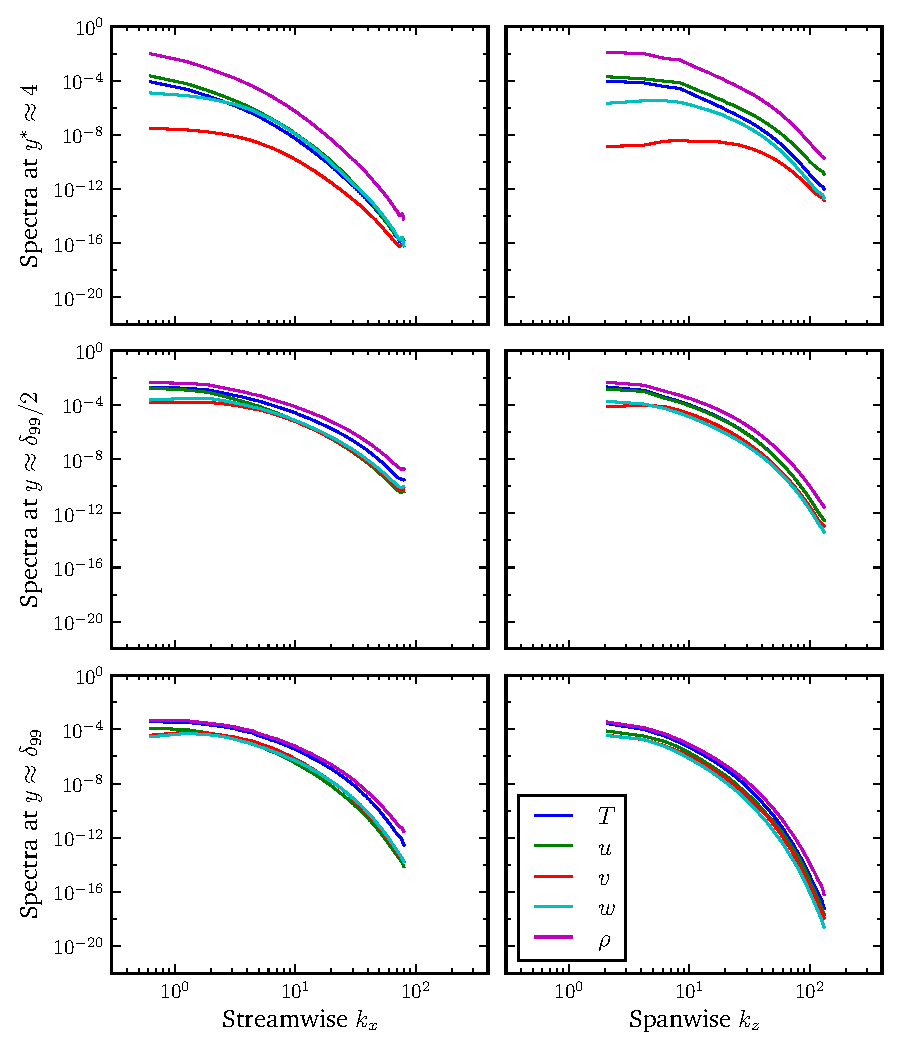
\includegraphics[width=\textwidth]{spectra-redux2299}
\caption{%
    One-dimensional, unnormalized Fourier energy spectra from an ensemble
    over the location 2.299~m data appearing in
    \autoref{fig:redux2299}.\label{fig:spectra-redux2299}
}
\end{figure}

\begin{figure}
\centering
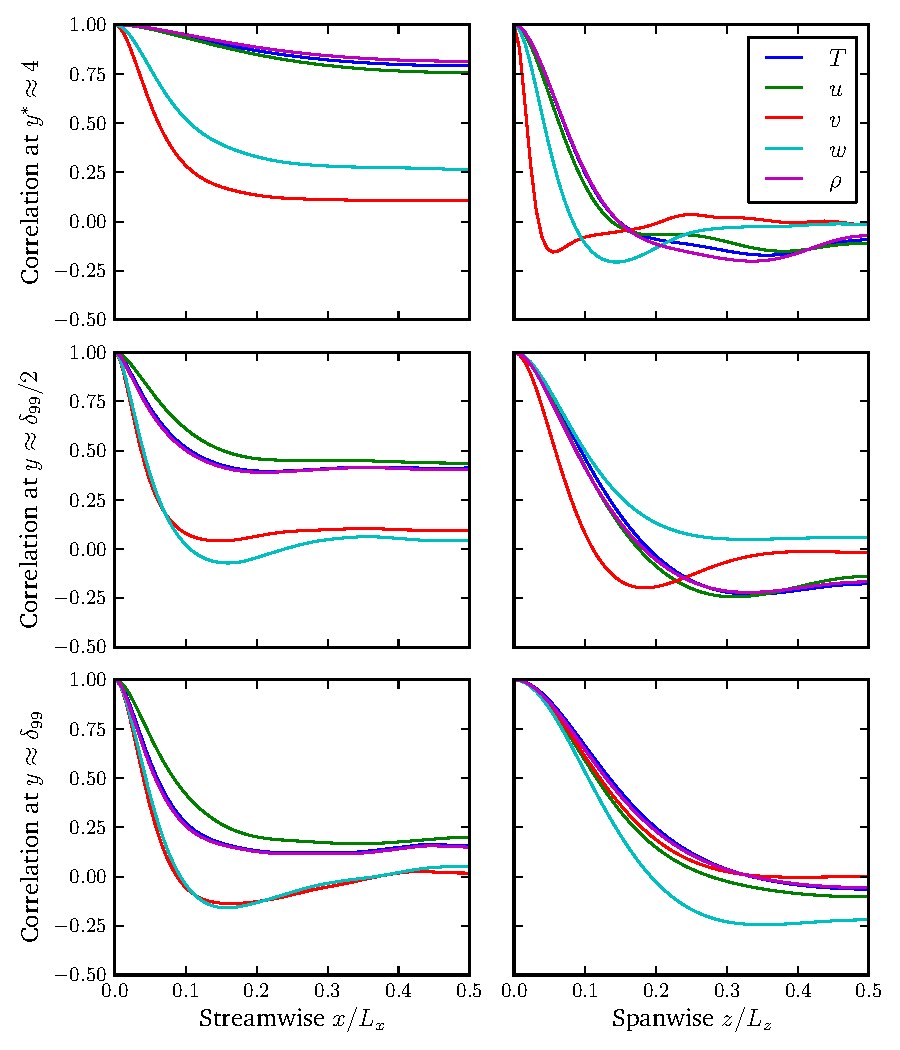
\includegraphics[width=\textwidth]{autocorr-redux2299}
\caption{%
    Two-point correlations from an ensemble over the location 2.299~m data
    appearing in \autoref{fig:redux2299}.\label{fig:autocorr-redux2299}
}
\end{figure}

\begin{figure}
\centering\includegraphics[width=\textwidth]{relam1389}
\caption{Refinement of exploratory simulation for location 1.389~m.\label{fig:relam1389}}
\end{figure}


%%%%%%%%%%%%%%%%%%%%%%%%%%%%%%%%%%%%%%%%%%%%%%%%%%%%%%%%%%%%%%%%%%%%%%%%%%%%%%
\clearpage
\subsection{Results from Fully Turbulent Initial Conditions}
\label{sec:relam_results_turb}

Not one of the post-refinement cases from the prior section used an
initial field known to demonstrate salient turbulent boundary layer
features.  They are, nonetheless, informative.  In particular,
Figures~\ref{fig:relam4134} and~\ref{fig:relam3199} suggest that conditions
4.134~m and 3.199~m both will relaminarize starting from a proper initial field.

Figures~\ref{fig:redux4134} and~\ref{fig:redux3199} on
pages~\pageref{fig:redux4134} and~\pageref{fig:redux3199} investigate those
two locations using stationary turbulent fields from simulations t4.134 and
t3.199, documented in \autoref{sec:bldata}, as initial conditions.
%
Local conditions from \autoref{tbl:cevisslam_inputs} were achieved by setting
the necessary code inputs for initial fully turbulent fields with resolution
$512\times{}256\times{}256$.
%
Because the initial grids, designed for $\Reynolds[\theta]{}=380$ and
531 flows, are excessive for $\Reynolds[\theta]{}\approx225$ they were
coarsened as the simulations proceeded.
%
The 4.134~m case resolution was gradually brought down past
$384\times{}256\times{}192$, past $384\times{}192\times{}192$, and
finally to $256\times{}192\times{}128$ at $t\approx{}34$ where
$\Delta{}x^{+}\approx{}17.2$ and $\Delta{}z^{+}\approx{}10.3$.
%
This case relaminarized after 10.4 turnovers in contrast to 6 observed in
\autoref{fig:relam4134}.
%
The 3.199~m case was handled similarly but was reduced only as
far as $384\times{}192\times{}192$ at $t\approx{}20$ where
$\Delta{}x^{+}\approx{}13.2$ and $\Delta{}z^{+}\approx{}7.9$.
%
This case relaminarized after 13.2 turnovers in contrast to the 36.3 observed in
\autoref{fig:relam3199}.
%
Both simulations used resolutions similar to those in
\autoref{tbl:table_turb_hbl}, which were found adequate.
%
Qualitatively both cases show the same features as the earlier refinement study
did at these locations.  Namely, the supersonic case at 4.134~m smoothly
dissipated away while the subsonic case at 3.199~m had a longer dwell time
before a relatively quick collapse.

For the studied parametrization of Bauman's fully laminar Orion MPCV solution,
locations 4.134~m and 3.199~m represent the boundary layer conditions on the
thermal protection system \emph{a priori} expected most likely to sustain
turbulence.  They possess $\Reynolds[\theta]{}$ within 4.6\% of peak 236 (found
at 3.762~m), among the highest $\Mach$, $T_e/T_w$ within 0.8\% of peak 4.321
(found at 3.983~m), and among the lowest $v_w^{+}$.
%
Given that expectation, having observed 4.134~m and 3.199~m relaminarize from
fully turbulent initial conditions, and having discovered a field
able to sustain nontrivial fluctuations at 2.299~m, the study was halted.

Despite comments made at the end of \autoref{sec:relam_methods}, a subsequent
confirmation of the relaminarizations seen in Figures~\ref{fig:redux4134}
and~\ref{fig:redux3199} at higher resolutions and for larger box sizes was
not performed.  Those comments pertained to the need to assess the sensitivity
of the hypothetical edge of the turbulence sustaining region to changes in
discretization.  Having observed no such edge, that particular sensitivity
became irrelevant.

%Two other sensitivities instead became of interest.
%%
%The first sensitivity question, and the more important one to address, is if
%modifying the domain size changes whether or not some
%given local conditions can sustain turbulence.
%%
%Only examining the impact of choosing a larger domain is of physical interest
%because employing a smaller domain is well-known to encourage aphysical
%simulation artifacts to appear.\footnote{%
%    As is true of many DNS studies, the present work
%    already examined nearly the smallest suitable periodic box.
%}
%%
%Intuitively, a larger domain better approximates the ability of a turbulent spot
%or some other turbulence-inducing disturbance to ``exit'' the simulation by decreasing
%the fraction of the overall periodic domain with which that spot interacts.
%Accordingly, we believe enlarging the domain necessarily increases the tendency
%to relaminarize.
%%
%The second sensitivity question is whether enlarging the domain impacts the time
%to relaminarize.  We suspect, per the same intuition, that larger domains take
%less time to relaminarize.  However, the matter was not pursued as it
%does not impact the following discussion.

\begin{figure}
\centering\includegraphics[width=\textwidth]{redux4134}
\caption{Fully turbulent initial condition study for location 4.314~m.\label{fig:redux4134}}
\end{figure}

\begin{figure}
\centering\includegraphics[width=\textwidth]{redux3199}
\caption{Fully turbulent initial condition study for location 3.199~m.\label{fig:redux3199}}
\end{figure}

%%%%%%%%%%%%%%%%%%%%%%%%%%%%%%%%%%%%%%%%%%%%%%%%%%%%%%%%%%%%%%%%%%%%%%%%%%%%%%
\clearpage
\section{Discussion}
\label{sec:relam_discussion}

Given the Orion MPCV boundary layer characterization in
Figures~\ref{fig:cevisslam_summary1} and~\ref{fig:cevisslam_summary_fpg}, that
local conditions at 4.134~m and 3.199~m relaminarized from fully turbulent
initial conditions, as shown in Figures~\ref{fig:redux4134}
and~\ref{fig:redux3199}, suggests no turbulence sustaining region exists on this
particular thermal protection system surface in this particular reentry scenario
according to the present modeling applied per the chosen methodology.  Those two
locations possess among the highest $\Reynolds[\theta]$ found in the Orion MPCV
International Space Station return scenario combined with weak $v_w^{+}$ and
$p_{e,\xi}^\ast$ and were \emph{a priori} anticipated to sustain turbulence if
any portion of the boundary layer could.

How robust is accepting the possible conclusion that the Orion
MPCV is fully laminar in this scenario with respect to using that information to predict aerothermodynamic
heating?  By using turbulent initial conditions in a periodic domain as a
surrogate for a fluctuation-rich flight environment, our methodology attempted
to capture that the reentry vehicle is awash in perturbations from the
freestream, from aerothermochemistry, from ablator outgassing, and from surface
roughness.  Setting aside concerns regarding the verisimilitude of the
homogenized governing equations, the robustness of a fully laminar conclusion
depends to a large extent on whether or not the turbulent initial condition
surrogate was adequate.

Drawing on the nonlinear stability theory discussed in
\autoref{sec:energyperturbationtheory}, turbulent initial conditions were
adopted for the relaminarization study because they are physically relevant but
moreso because they represent large, potentially self-sustaining disturbances
relative to laminar flows.
%
The discovery of the field able to sustain nontrivial
fluctuations at 2.299~m, pictured in \autoref{fig:redux2299}, demonstrates that
turbulent initial conditions were not the most conservative possible way to
emulate a fluctuation-rich flight environment for the purposes of determining
where local conditions can sustain turbulence.  Heightened conservatism is appropriate
because in-flight perturbations cannot be characterized well-enough to apply
transition models as discussed in \autoref{sec:transition}.
%Therefore, though the 2.299~m field was clearly not physical, we believe
%its discovery is germane

Consequently, despite relaminarization from turbulent initial
conditions at 4.134~m and 3.199~m, the existence of a long-lived,
fluctuating field at 2.299~m forces us to conservatively conclude that
the turbulence-sustaining region on the Orion MPCV extends from the
edge of the thermal protection system to at least 2.299~m leeward of
the stagnation point.  Having observed location 1.389~m relaminarize
from initial conditions like those that generated the fluctuation-sustaining
2.299~m field,
we conclude that the turbulence
sustaining region does not extend to within 1.389~m leeward of the
stagnation point.  That conclusion is predicated on the
homogenized governing equations providing accurate predictions regarding
the turbulence-sustaining behavior of spatially evolving boundary layers
which has not been validated in the present work.

Where between locations 1.389~m and 2.299~m is the edge of the turbulence
sustaining region?  We suspect it lies closer to 2.299~m but we do not know
conclusively.
%
Investigating that interval will require a more sophisticated way than
crude auxiliary simulations to determine the code inputs necessary to
incrementally bring the
fluctuation-sustaining 2.299~m field inward towards the stagnation point.
%
Two suggestions were already made in \autoref{sec:relam_methods}.
%
%Indeed, though not shown in the results section, it took three separate attempts
%from \autoref{fig:relam2299} to better achieve its target conditions in
%\autoref{fig:redux2299}.
%
Calibrating a turbulence model equipped with spatiotemporal homogenization terms
to reproduce statistics from the fluctuation-sustaining 2.299~m field appears to be a
necessary first step towards either suggestion.

One factor contributing to the difficulty of obtaining code parameters to
match such local conditions was the implicit dependence of $v_w^{+}$ on
all code inputs.  The present study targeted a constant $v_w^{+}$ based
on conditions found in Bauman's fully laminar Orion MPCV simulation.
The metric was selected because it approximated outgassing from a
steady ablative heat shield.  As can be seen from the results,
the normalized wall blowing became stronger as simulations relaminarized.
A better approach for future work may be to control $v_w/u_0$ to match the
local nondimensional heat flux $B_q$~\citep{Bradshaw1977Compressible}
from MPCV data.
Matching the heat flux approximates an ablator able to react to flow
conditions.  Care is required, however, to not have the controller
mechanism introduce undesirable time scales into the simulation.
%\footnote{%
%    The idea of using a controller to hold $\delta_{99}/l_0\approx{}1$
%    was entertained long enough to prepare an implementation
%    (\url{https://github.com/RhysU/helm}) along with much of the
%    required infrastructure within Suzerain.  The idea was abandoned
%    after coming to believe turning the controller for this study
%    would require time commensurate with simply adjusting the
%    $\operatorname{gr}_{t_0}\left(\Delta\right)$ and, done hurriedly,
%    could destabilize the simulations.
%}

It would be interesting to repeat the \citet{Bauman2011Loose} heat shield
simulations with turbulence tripped at 1.389~m and to compare the result with
both \autoref{fig:normalized_difference} and \autoref{tbl:BaumanCEVConditions}.
That prediction could be contrasted with heating data gathered during the
upcoming NASA Exploration Flight Test-1~\citep{SpaceCom20140317} in the hope
that the simulation matches evidence of where on the heat shield
turbulence-enhanced energy transport is present.
%
However, a comparison may not be straightforward as that flight test will use a
different reentry trajectory than the peak heating regime studied here.

Finally, if one wanted to limit a relaminarization study to only fully turbulent
initial conditions and possibly find a turbulence-sustaining edge, the higher
speed Exploration Flight Test-1 trajectory may be ideal.  Studying a faster
trajectory with the suggested methodology improvements may allow interrogating
the physics at the cusp where turbulence can only barely be sustained.


\chapter{Conclusions}
\label{sec:conclusions}

The objective of this research project is to provide a definitive
assessment of the technological feasibility of the entire synthetic
columnar vortex concept as a means of generating usable energy. In the 
previous sections outlined the present state of the
simulation capability. In doing so, we have discussed the physics that
influence dust devils formation, our particular mathematical
models for the ambient conditions, as well as the SoV vanes, cone and
turbine. We summarized the numerical discretizations used, the software
stack and the calibration, verification and validation of these
components. The purpose of these sections was to communicate
two major points. The first is that an accurate, verified and
validated simulation capability has been developed that can quickly
investigate a wide variety of system and scenario settings at a modest
computational cost. The second point is that we have developed
heuristics that permit optimization of any baseline SoV configuration to
a local maximum of energy production, as measured by kinetic energy flux
through the top of the SoV vanes.  

These two points justify the proposed course of work, which is to
explore a large space of possible system configurations
and geometries to discover the globally optimal structure
of the SoV apparatus. Coupled with the scaling analysis presented in
Section \ref{sec:physics}, we will then be able to predict the
conditions (if any) under which the SoV apparatus will be
technologically feasible. This will lead to investigating the physics of the
apparatus, to assess how closely the synthetic dust devils mimic the
natural variety. The proposed research is designed to
assess feasibility, and it is not expected that actual experimental
validation will accompany the computational results. Furthermore, it
must also be emphasized that feasibility is focused on
technical viability, namely energy produced by the apparatus,
and will not include an economic assessment. In other words, it is
possible that the SoV will produce energy, but the design required to do
is prohibitively expensive, and therefore not economically competitive
with existing technologies. The following is a proposed program of simulations 
designed to explore a wide configuration space. This focuses on
optimization for the cone, turbine and vanes. 

%
% vane optimization
%
%% \large
%% \begin{center}
%% \begin{table}[h]
%%  \centering
%%   \begin{tabular}{| l | c | l |}
%%     \hline
%%     Parameter & Description & Range \\
%%     \hline
%%     $\theta^{\text{t}}_{\text{min}}$ & Starting, minimum angle of the
%%        top tier & ( 0 - $\theta^{\text{t}}_{\text{max}}$ ) \\
%%     $\theta^{\text{t}}_{\text{max}}$ & Ending, maximum angle of the top
%%        tier & ( 0 - 90 ) \\
%%     $\theta^{\text{b}}_{\text{min}}$ & Starting, minimum angle of the
%%        bottom tier & ( 0 - $\theta^{\text{b}}_{\text{max}}$ ) \\
%%     $\theta^{\text{b}}_{\text{max}}$ & Ending, maximum angle of the
%%        bottom tier & ( 0 - 90 ) \\
%%    $\gamma^t$ & Rate of curving, vane top tier & ( 0 - 3 ) \\
%%    $\gamma^b$ & Rate of curving, vane bottom tier & ( 0 - 3 ) \\
%%    $1 - (r_{\text{min}} / r_{\text{max}})^{\text{t}}$ & Length of the top
%%        tier vane & ( 0 - 1 ) \\
%%    $1 - (r_{\text{min}} / r_{\text{max}})^{\text{b}}$ & Length of the
%%        bottom 
%%        tier vane & ( 0 - 1 ) \\
%%    $H^b/H^t$ & Ratio of heights between bottom and top tiers & ( 0 -
%% 	   0.5 ) \\ 
%%    $D/H$ & Ratio of apparatus diameter and total vane height & ( 0.5 -
%% 	   5.0 ) \\ 
%%     \hline
%%   \end{tabular}
%%   \caption{Vane Optimization Parameters.}
%%   \label{tab:vane}
%% \end{table}
%% \end{center}
%% \normalsize\todo{keep table?}

The three cone parameters we propose to optimize are shown in Table
\ref{tab:cone}. We expect to optimize the cone after the bottom and top
tiers are adjusted. For the cone, we expect the height, maximum diameter
and inner exit diameter to all impact the flow. While it is not known
what form the ideal cone geometry will take, our expectation is that the
cone plays at least two important roles. The first is acting as a
converging nozzle for the flow, increasing the vertical and azimuthal
velocity as it exits out the top of the device. In the wind, the cone
also acts as a shield, preventing the high velocity freestream flow from
disrupting the vortex before it has run through the turbine. 

%
% cone optimization
%
\large
\begin{center}
\begin{table}[h]
 \centering
  \begin{tabular}{| l | c | l |}
    \hline
    Parameter & Description & Range \\
    \hline
    $H_C/D_C$ & Ratio of the height of the cone versus the cone diameter & ( 0 - 2.0 ) \\
    $D_{\text{C}}/D$ & Ratio of the cone diameter versus the system
       diameter & ( 0.5 - 1.5 ) \\
    $D_{\text{out}}/D_C$ & Ratio of the cone exit diameter versus the
       cone diameter & ( 0.25 - 1.0 ) \\ 
    \hline
  \end{tabular}
  \caption{Cone Optimization Parameters.}
  \label{tab:cone}
\end{table}
\end{center}
\normalsize

The turbine parameters to be optimized are shown in Table
\ref{tab:turbine}. In addition to these configuration parameters, the
location of the turbine will likely need to be optimized to be centered
on the vortex, which may not be centered inside the vanes due to
asymmetric effects of wind, vane geometry, etc. 

%
% turbine optimization
%
\large
\begin{center}
\begin{table}[h]
 \centering
  \begin{tabular}{| l | c | l |}
    \hline
    Parameter & Description & Range \\
    \hline
    $N_B$ & Number of blades & ( 1 - 12 ) \\
    $I$ & Moment of inertia & ( 1 - 12 ) \\
    $r_B/r_{\text{min}}^t$ & Radius of blade versus the inner radius of
       the top tier vanes & ( 0 - 1 ) \\
   $H_B/H$ & Height of the turbine blades versus system height & ( 0 - 1.2 ) \\
    \hline
  \end{tabular}
  \caption{Proposed Turbine Optimization Parameters.}
  \label{tab:turbine}
\end{table}
\end{center}
\normalsize

The possible configuration space for the vanes is much larger. 
Presently, the workflow consists of weekly calls with the experimental
team to discuss possible system designs, which typically consist of vane
sketches or drawings. One such proposed design is shown in Figure
\ref{fig:sketch}.  These vanes are highly asymmetric with variation in
the length and curvature as a function of spatial location. Furthermore,
in this design the down wind side of the apparatus is enclosed by a
solid cylindrical wall.  While the vane representation outlined in
Section \ref{subsec:vane} is expected to be sufficiently general to support a
wide variety of vane configurations, it is not at this time clear what
form of parameterization for vane angle is sufficiently general to
support this exploration, and so a table like that for the cone and
turbine is not yet available. At present the expectation is to proceed
with this conceptual phase to generate a wide  range of possible
configurations. The designs that have initially promising results will
then be optimized similar to the examples outlined in Section
\ref{sec:results}, where new parameter values are 
introduced, a run is performed, and then the output is postprocessed and
evaluated before the process begins again. In this way it is not
infeasible to expect that several hundred optimization runs can be
performed. 
%The next subsection also briefly outlines a proposal to
%investigate algorithmic optimization on these designs.  

\begin{figure}[htb]
 \centering
 \includegraphics[width=.75\linewidth]{figs/top}
 \caption{This is an example image of a proposed vane design. The lines
 indicate the vane curvature and solid surfaces. Sketches and diagrams
 such as this  are typically generated by various members of the
 team. The vane surface is then instantiated as a region of forcing as
 detailed in Section \ref{subsec:vane} and then simulated. If the
 initial results are promising, then further exploration of that
 configuration may be pursued.} 
 \label{fig:sketch}
\end{figure}



% Table \ref{tab:vane} lists the proposed optimization parameters for the
% vanes. We propose nine parameters to optimize for the
% vanes. $\theta^{\text{t}}_{\text{min}}$ and
% $\theta^{\text{b}}_{\text{min}}$ are the top and bottom tier minimum
% angles. This is essentially the starting (and minimum) angle for the curved
% vanes. Preliminary investigations have given no indication that the
% bottom tier is receptive to anything but a fully radial angle
% (e.g. $0^{\circ}$). For the top tier, however, a non-zero
% $\theta_{\text{min}}$ has been found to increase the kinetic energy
% flux. For both of the maximum angles we have reasonable starting
% points. Previously, we have found that a larger angle at the bottom tier
% is ideal, as it serves to ``spin-up'' a small core region.

% We have less strongly informed prior expectations of reasonable values
% for the rate of curvature, $\gamma$, the ratio of heights between the
% top and bottom tiers ($H^b/H^t$) as well as the lengths of the
% vanes. The generated flux is certainly sensitive to $\gamma$, but
% optimal value is certainly not known. Likewise, while we have operated
% with shorter vanes lengths on the top than the bottom, as well as a
% shorter height, we are not certain that these configurations are
% remotely optimal. Finally, for $D/H$, the ratio between the apparatus
% diameter and total vane height, we have only operated near a ratio of
% 1.0. However, as noted in \cite{ROG:ROG1635}, ``Most dust devils are at 
% least 5 times higher than they are wide''. While increasing the height
% of the apparatus would greatly increase the cost and inaccessibility of
% the device for maintainance, this indicates that it is necessary to
% examine the dependence of energy produce by the vortex at greater system
% heights. We expect to increase beyond this aspect ratio of $\approx 1$
% towards the naturally occuring ratio of 5. If this is found to greatly
% enhance energy output, we will then consider even larger
% ratios.\todo{add image}
%
% need to expand this to discuss huge space of vanes
% add image too?
%



%\subsection{Risks and Challenges to the Optimization Efforts}

%% A challenge inherent to this optimization effort is that while the
%% principle quantity of interest is the kinetic energy flux, we also seek
%% to use these runs to shed light on the mechanisms by which the apparatus
%% configuration dictates the flow. In other words, we are trying learn
%% more than \textbf{which} configurations optimize the flow, but also 
%% \textbf{why} they do so. 

% This presents an programmatic challenge, as
% optimization will involve additional analysis and postprocessing at each
% iteration.  

%
% how many runs are we capable of performing, realistically
% largely obsolete!

% An additional challenge is the computational expense of each run. 
% Each parameter exploration requires approximately 12 wall-clock hours to run
% the simulation for a sufficient time to pass any initial transient in
% the solution and then permit adequate statistical averaging at steady
% state. Runs generally require approximately 264 processors on Lonestar
% (for example) and therefore the cost of a forward run is $\approx 3,200$
% core hours. Our overall compute budget will likely be between one hundred
% thousand to one million core hours. In other words, our present
% computational budge will support running between roughly 30 to 300
% instances for our parameter sweeps. While this is not insubstantial, this
% is not a sufficient number of evaluations to support formal
% optimization algorithms. While we admittedly do not, \textit{a priori},
% know the number of iterations necessary to solve the system, as it is
% non-linear, our expectation is that thousands of forward solves would be
% necessary. Using higher order methods could reduce the number of
% iterations, but gradient and derivative information is difficult to
% access, as solving the adjoint problem is expensive for unsteady systems. 
% Thus, while any individual run is relative inexpensive, we do not expect
% to be able to mount an exhaustive campaign to formally optimize the
% configuration given the dimension of the parameter space and the
% structure of the problem. 

%
% introduce concept of subdomains
%

% Furthermore, the time requires to perform this simulation campaign could
% be greatly reduced if several problems were to be undertaken in
% parallel. This ``divide and conquer'' approach requires subdividing the
% optimization effort into several ``subdomains''. 
% The problem is nonlinear, and so some of the parameters are coupled and
% cannot be easily optimized independent of each another, as adjustments
% to one impact the desired value of the other. 
% We propose to subdivide the vanes into upper and lower tiers, optimize
% them individually, and then perform rudimentary sensitivity checks to
% ensure that the coupled product does in fact represent a near optimal
% flux output. We further expect that the remaining parameters in the
% vanes, namely $H^b/H^t$, $D/H$ are amenable to optimization independent
% of the particular parametric configuration of the vane tiers. 

% The subdomains for the vanes are are summarized in Table
% \ref{tab:opt}. This neatly divides the vane optimization effort into
% three independent problems with 4 or fewer parameters each.

% \begin{center}
% \begin{table}[h]
%  \centering
%   \begin{tabular}{|l | l | l |}
%    \multicolumn{3}{c}{Subdomains} \\
%     \hline
%    Top Tier & Bottom Tier & Misc. \\
%    \hline
%    $\theta^{\text{t}}_{\text{min}}$ & $\theta^{\text{b}}_{\text{min}}$ &
%        $H^b/H^t$ \\
%    $\theta^{\text{t}}_{\text{max}}$ & $\theta^{\text{b}}_{\text{max}}$&
% 	   $D/H$ \\ 
%    $\gamma^t$ & $\gamma^b$ & \\
%    $1 - (r_{\text{min}} / r_{\text{max}})^{\text{t}}$ & $1 -
%        (r_{\text{min}} / r_{\text{max}})^{\text{b}}$ & \\
%    \hline
%   \end{tabular}
%   \caption{Vane optimization parameters, divided into parallelizable
%  subdomains.} 
%   \label{tab:opt}
% \end{table}
% \end{center}

\subsection{Proposed Timeline}

%
% timeline
%
A timeline for the proposed work is presented in Table
\ref{tab:prop}. The date of each bullet is the planned completion of the
deliverable. Bullets items in black are required, while those in blue
are optional, and do not need to be completed to ensure the
success of this project. 

% 
% can we optimize? DAKOTA
% 
% We propose to investigate algorithmic optimization as a tool to discover
% locally optimal system configurations. 
% This will take the form of using either the DAKOTA\cite{adams2013dakota}
% or TAO\cite{tao-user-ref} libraries. These libraries have suites of
% algorithms for non-linear optimization problems without gradient
% information (derivative-free optimization, such as Nelder-Mead or downhill simplex methods). 
% Evaluating the results of the most
% appropriate ``out of the box'' available optimization algorithm on a
% small test problem will provide an opportunity to ensure that our
% expectations on the number of iterations necessary for formal
% optimization of our problem are reasonably correct. 
% We propose these two libraries because DAKOTA is well-known as a library
% with extensive ``black-box'' optimization support, and TAO is already
% made available through pre-existing libMesh dependencies. Should the
% test problem discover that algorithmic optimization is a viable option,
% we will consider using this approach for optimization of the
% configuration. 

%
% short summary of tasks
%

The first bullet in Table \ref{tab:prop} provide
estimated ending dates for the exploration of the configuration space. 
We have rapidly iterated 
through these optimization efforts over the course of several
months, and are nearly converged on a final design. 
The second bullet relates to the the final verification of the turbine, to ensure
this functions properly. 
At this time we will proceed with ``coupling tests'' to 
ensure that the parameters are indeed still appropriate. For example,
after having optimized the turbine parameters, it may be necessary to
perturb the lower tier vane parameters to ensure that the selected set
is nearly optimal even with the addition of a turbine. 

%
% probably ok below:
%
The third bullet is the expected deadline to provide the results of our
computational simulation efforts to the experimental group in late
Spring/early Summer of 2016 so that they can use this information in the
design of the system to be used for the Arizona field tests in Summer,
2016. The date of the actual field test has not yet been set and may change. 

As mentioned in the fourth item, it is possible that this
project will permit some glimpses  
at the fundamental processes underlying the naturally dust devil
phenomena. To accomplish this, the synthetic dust devils must be
compared to data from the naturally occuring variety,  with some
appropriate scaling. While it is not a significant component of the
proposal, this and several simple investigations into related phenomena
such as tornados and hurricanes will also  be investigated. A literature
review of the physics of general cyclonic structures and any observed
intensification mechanisms may provide hints of the geometries 
by which the flow is intensified, and why. 

Given our previous experiences, we do not anticipate a rich validation data set 
to be available after the field test. Nevertheless, we will postprocess any and all
available data from this event in order to assess the reliability of the computational
modeling efforts. 

Finally, we anticipate a detailed accounting of the entire project as
the final deliverable. We expect that all of the investigations detailed 
above will result in several publications, as well. 

%
% itemize tasks
%
% In summary, in addition to the preliminary results, several tasks will be
% accomplished  to fulfill the goals of this project:

% \begin{itemize}
%  \item validate turbine
%  \item numerous optimization runs
%  \item best guess of ideal run (possible field run)
%  \item feasibility study?
% \end{itemize}

\begin{center}
\begin{table}
\caption{Timeline of proposed work. Bullets are dates of planned
 completion of deliverables. Black items are requisite, blue optional.}
\centering
\begin{minipage}[t]{.7\linewidth}
\color{black}
\rule{\linewidth}{1pt}
\ytl{April 2016}{Conclude parameter sweeps and optimization of apparatus}
\ytl{April 2016}{Turbine actuator-disk verification, validation and prediction}
\ytl{May 2016}{Proposed configuration and predictions for experimental
 team}
\ytb{July 2016}{Comparisons between synthetic and natural dust devil physics}
\ytl{Aug 2016}{Validation against 2016 field data}
%\ytl{Aug 2016}{SoV feasibility assessment}
\ytl{Fall 2016}{Doctoral dissertation writing}
\bigskip
\rule{\linewidth}{1pt}%
\end{minipage}%
\end{table}
\label{tab:prop}
\end{center}

% \subsection{Additional Investigations}

% % 
% % control for inter unit spacing
% % 
% In addition to the system configuration, it would be interest to consider the
% effect of local conditions on SoV performance. Characterizing the impact
% of variations in ambient conditions on the SoV will guide the
% commercialization strategy of the product, by determining optimal
% install locations across the country. It is therefore desirable to have
% models that are capable of accounting for variation in field conditions,
% such as solar input, cross-winds and topography. Furthermore, it is
% expected that large ``farms'' of SoVs (akin to the wind and solar farms
% for wind turbines and photovoltaics, respectively) may be used by
% commercial or utility-scale energy generation. For this to be
% effective,  the inter-unit spacing must also be optimized, as a single
% SoV collects from a large area. These computations will guide
% commercialization planning, where decision-makers will need to assess
% optimum unit size, spacing, and geographic location for utility-scale
% deployment.   


%%%%%%%%%%%%%%%%%%%%%%%%%%%%%%%%%%%%%%%%%%%%%%%%%%%%%%%%%%%%%%%%%%%%%%
% Appendix/Appendices                                                %
%%%%%%%%%%%%%%%%%%%%%%%%%%%%%%%%%%%%%%%%%%%%%%%%%%%%%%%%%%%%%%%%%%%%%%
%
% If you have only one appendix, use the command \appendix instead
% of \appendices.

\appendices
%%\appendix

\chapter{Derivation of the Mathematical Models}
\label{sec:derivation}

Here the mathematical models summarized in \autoref{sec:model} are derived.
While the first two sections containing the Navier--Stokes and Favre-averaged
Navier--Stokes equations are classical and straightforward, the derivations are
provided to document the few peculiar constitutive choices as well as to
unambiguously fix nomenclature.  The third section documents a new
spatiotemporal homogenization approximation by \citet{Topalian2014Spatiotemporal}.
%
Dimensional equations are employed throughout this appendix.  The final
dimensional summary in each of the following subsections is nondimensionalized
to arrive at the formulations used in the main body of the dissertation.

\section{The Governing Equations}

\subsection{Conservation Laws}

%\subsubsection{Reynolds transport theorem}
Consider a time-varying control volume $\Omega$ with surface
$\partial\!\Omega$ and unit outward normal $\hat{n}$.  For any
scalar, vector, or tensor field quantity
$T$, Leibniz' theorem states
\begin{align}
  \label{eq:rtt}
  \frac{d}{dt}\int_{\Omega(t)}T(x,t)\,dV
  &=
  \int_{\Omega}\frac{\partial\!}{\partial\!t}T\,dV
  +
  \int_{\partial\!\Omega} \hat{n}\cdot{}w T\,dA
  =
  \int_{\Omega}\frac{\partial\!}{\partial\!t}T+\nabla\cdot{}wT\,dV
\end{align}
where $w$ is the velocity of $\partial\!\Omega$.  When $\Omega$ follows
a fixed set of fluid particles, $w$ becomes the fluid velocity $u$.

%\subsubsection{Conservation of Mass}
Since mass $M=\int_{\Omega} \rho\,dV$
and mass conservation requires $\frac{d}{dt}M=0$,
\begin{align}
  0 = \frac{d}{dt}M
  = \frac{d}{dt}\int_{\Omega} \rho\,dV
  =
  \int_{\Omega}\frac{\partial\!}{\partial\!t}\rho+\nabla\cdot{}u\rho{}\,dV.
\end{align}
Because the result holds for any control volume, locally it must be true
that
\begin{align}
  \label{eq:cons_mass}
  \frac{\partial\!}{\partial\!t}\rho+\nabla\cdot\rho{}u &= 0.
\end{align}

%\subsubsection{Conservation of Momentum}
Separating total force into surface forces and body forces,
\begin{align}
  \sum{}F
  &=
     \int_{\partial\!\Omega} f_s \, dA
   + \int_{\Omega} f \, dV
  =
     \int_{\partial\!\Omega} \sigma \hat{n} \, dA
  +  \int_{\Omega} f \, dV
  =  \int_{\Omega} \nabla\cdot\sigma + f \, dV
\end{align}
where $\sigma$ is the Cauchy stress tensor.  From linear momentum
$I=\int_{\Omega} \rho{}u\,dV$ and its conservation $\frac{d}{dt}I=\sum{}F$,
\begin{align}
    \int_{\Omega}\frac{\partial\!}{\partial\!t}\rho{}u
  + \nabla\cdot(u\otimes{}\rho{}u)\,dV
&= \int_{\Omega} \nabla\cdot\sigma + f \, dV
.
\end{align}
As the control volume may be arbitrary,
\begin{align}
  \frac{\partial\!}{\partial\!t}\rho{}u + \nabla\cdot(u\otimes{}\rho{}u)
&= \nabla\cdot\sigma + f
.
\end{align}
Lastly, separating the pressure $p$ and viscous contributions $\tau$ to
the Cauchy stress tensor so that $\sigma = -p I + \tau$,
\begin{align}
\label{eq:cons_momentum}
\frac{\partial\!}{\partial\!t}\rho{}u + \nabla\cdot(u\otimes{}\rho{}u)
&= -\nabla{}p + \nabla\cdot{}\tau + f
.
\end{align}
The conservation of angular momentum implies $\sigma=\trans{\sigma}$ and
therefore $\tau=\trans{\tau}$ too.

%\subsubsection{Conservation of Energy}
Combining internal and kinetic energy into an intrinsic density $E$,
energy $\mathscr{E}$ is
\begin{align}
  \mathscr{E} &= \int_{\Omega} \rho{}E \, dV
  .
\end{align}
Treating heat input $Q$ as both a surface phenomenon described by an outward
heat flux $q_{s}$ and as a volumetric phenomenon governed by a
body heating $q_{b}$,
\begin{align}
  Q
  &=
   \int_{\Omega}\rho{}q_{b}\,dV
  -\int_{\partial\!\Omega}\hat{n}\cdot{}q_{s}\,dA
  =
    \int_{\Omega}q_{b} - \nabla\cdot{}q_{s}\,dV
  .
\end{align}
Power input $P=F\cdot{}v$ accounts for surface stress work and body
force work to give
\begin{align}
  P
  &=
    \int_{\partial\!\Omega} \sigma{}\hat{n} \cdot{} u \, dA
  + \int_{\Omega} f \cdot{} u \, dV
  = \int_{\Omega} \nabla\cdot{}\sigma{}u + f \cdot{} u \, dV
  .
\end{align}
Demanding energy conservation $\frac{d}{dt}\mathscr{E}=Q+P$,
\begin{align}
  \int_{\Omega}\frac{\partial\!}{\partial\!t} \rho{}E
  +
  \nabla\cdot{}u\rho{}E
  \,dV
&=
    \int_{\Omega} q_{b} - \nabla\cdot{}q_{s}\,dV
  + \int_{\Omega} \nabla\cdot\sigma{}u + f \cdot{} u \, dV
  .
\end{align}
Again, since the control volume was arbitrary,
\begin{align}
  \frac{\partial\!}{\partial\!t} \rho{}E
  +
  \nabla\cdot{}\rho{}Eu
&=
  - \nabla\cdot{}q_{s}
  + \nabla\cdot\sigma{}u
  + f \cdot{} u
  + q_{b}
  .
\end{align}
Splitting $\sigma$'s pressure and viscous stress contributions into separate
terms,
\begin{align}
  \label{eq:cons_energy}
  \frac{\partial\!}{\partial\!t} \rho{}E
  +
  \nabla\cdot{}\rho{}Eu
&=
  - \nabla\cdot{}q_{s}
  - \nabla\cdot{}pu
  + \nabla\cdot{}\tau{}u
  + f \cdot{} u
  + q_{b}
  .
\end{align}

\subsection{Constitutive Assumptions}
\label{sec:constitutive}

%\subsubsection{Perfect gas}

Assume the fluid is a thermally and calorically perfect gas governed by
\begin{align}
  \label{eq:perfectgaseos}
  p &= \rho{} R T
\end{align}
where $R$ is the gas constant. The constant volume $C_{v}$ specific heat,
constant pressure specific heat $C_{p}$, and acoustic velocity $a$
relationships follow:
\begin{align}
  \label{eq:perfectgasrelations}
  \gamma &= \frac{C_{p}}{C_{v}}
  &
  C_{v} &= \frac{R}{\gamma - 1}
  &
  C_{p} &= \frac{\gamma{}R}{\gamma-1}
  &
  R &= C_{p} - C_{v}
  &
  a^{2} = \gamma{}RT.
\end{align}
Also assume $C_{v}$ and $C_{p}$ and, therefore, $\gamma$ are constant.
The total (internal and kinetic) energy density is
\begin{align}
  \label{eq:perfectgastotalenergy}
  E &= C_{v} T + \frac{1}{2}u^{2}
     = \frac{RT}{\gamma-1} + \frac{1}{2}u^{2}
\end{align}
where the notation $u^2 = u\cdot{}u$ is employed.
The total enthalpy density $H$ and (internal) enthalpy density $h$ are
\begin{align}
  \label{eq:perfectgasenthalpy}
  H &= E + \frac{p}{\rho}
     = C_{p} T + \frac{1}{2}u^{2}
     = \frac{\gamma{}RT}{\gamma-1} + \frac{1}{2}u^{2},
\\
  h &= H - \frac{1}{2}u^{2}
     = C_{p} T
     = \frac{\gamma{}RT}{\gamma-1}
  .
\end{align}
See a gas dynamics reference, for example \citet{LiepmannRoshko2002}, for more
details.

%\subsubsection{Newtonian fluid}
\label{sec:newtonianfluid}

If one seeks a constitutive law for the viscous stress tensor $\tau$
using only velocity information, the principle of material frame
indifference implies that uniform translation (given by velocity $u$)
and solid-body rotation (given by the skew-symmetric rotation tensor
$\omega=\frac{1}{2}\left( \nabla{}u-\trans{\nabla{}u} \right)$)
may not influence $\tau$.  Considering contributions only up to the
gradient of velocity, extensional strain (dilatation) and shear strain
effects may depend on only the symmetric strain rate tensor
$\varepsilon=\frac{1}{2}\left( \nabla{}u+\trans{\nabla{}u}\right)$
and its principal invariants.

Assuming $\tau$ is isotropic and depends linearly upon only $\varepsilon$,
express it as
\begin{align}
\tau_{ij}
&= c_{ijmn} \varepsilon_{mn}
\notag \\
&= \left( A \delta_{ij} \delta_{mn}
        + B \delta_{im} \delta_{jn}
        + C \delta_{in} \delta_{jm}
    \right) \varepsilon_{mn}
&
&\text{for some }A, B, C\in\mathbb{R}
\notag \\
&= A \delta_{ij} \varepsilon_{mm} + B\varepsilon_{ij} + C\varepsilon_{ji}
\notag \\
&= A \delta_{ij} \varepsilon_{mm} + \left( B+C \right)\varepsilon_{ji}
\notag \\
&= 2 \mu \varepsilon_{ij} + \lambda\delta_{ij}\nabla\cdot{}u
\end{align}
where $\mu=\frac{1}{2}\left( B + C \right)$ is the dynamic coefficient of
viscosity (shear) and $\lambda=A$ is the second coefficient of viscosity
(dilatational).  Reverting to direct notation,
\begin{align}
\tau
&= 2 \mu \varepsilon + \lambda \left( \nabla\cdot{}u \right) I
\label{eq:taunewt}
 =   \mu \left( \nabla{}u + \trans{\nabla{}u} \right)
   + \lambda \left( \nabla\cdot{}u \right) I
.
\end{align}

The bulk viscosity $\mu_{B}=\lambda + \frac{2}{3}\mu$ and the deviatoric
part of the strain rate tensor,
\begin{align}
  S &= \varepsilon - \frac{1}{3} \trace\left(\varepsilon\right) I
     = \frac{1}{2}\left(\nabla{}u + \trans{\nabla{}u}\right)
     - \frac{1}{3}\left(\nabla\cdot{}u\right)I,
\end{align}
may be used to write
\begin{align}
\label{eq:tauSmub}
  \tau &= 2 \mu S + \mu_B  \left( \nabla\cdot{}u \right) I
.
\end{align}
The kinematic viscosity and bulk kinematic viscosity
\begin{align}
 \nu &= \frac{\mu}{\rho} & \nu_{B} &= \frac{\mu_{B}}{\rho}
\end{align}
are often used to simplify notation.

%\subsubsection{Stokes' hypothesis}
\label{sec:stokeshypothesis}

Set the bulk viscosity $\mu_{B}$ to be a fixed multiple of the dynamic
viscosity $\mu$.  This relationship may be written as either
\begin{align}
\label{eq:secondviscosityclaw}
\mu_{B} &= \alpha \mu
&
&\text{or}
&
\lambda &= \left( \alpha - \frac{2}{3} \right) \mu
\end{align}
where a dimensionless proportionality constant $\alpha$ has been introduced.
Stokes' hypothesis that bulk viscosity is negligible may be recovered by
selecting $\alpha = 0$.  Though Stokes' hypothesis is valid for most
circumstances~\citep{GadelHak1995}, we choose to separately track $\mu$ and
$\lambda$ terms in the model.

%\subsubsection{Power Law Viscosity}

Assume that viscosity varies only with temperature according to
\begin{align}
\label{eq:powerlawviscosity}
\frac{\mu}{\mu_{0}}=\left(\frac{T}{T_{0}}\right)^{\beta}
\end{align}
where $\mu_{0}$ and $T_{0}$ are suitable reference values.  This relationship
models air well for temperatures up to several thousand degrees
Kelvin~\citep{NASA-TR-R-132} as shown in \autoref{fig:Svehla1962}.
Sutherland's law~\citep{Sutherland1893Viscosity}, often recommended for its
greater accuracy~\citep[p. 46]{Smits2005Turbulent}, was avoided
because of the greater complexity its use would entail in expressions like
\eqref{eq:Tmonstrosity}.

\begin{figure}[tb]
\centering
\includegraphics[height=0.6\textwidth]{AirViscosityVsTemperature}
\caption[Viscosity of air versus temperature from 100 to 5000K]{%
    Power law fit for air viscosity versus temperature over 100 to 5000 K using
    data from \citet{NASA-TR-R-132}.  The least squares fit over this wide range
    is relatively insensitive to the chosen references $\mu_0$ and $T_0$.  For
    example, selecting $T_0 = 300K$ or $4000K$ causes exponents $0.6639$ or
    $0.6673$ to be optimal, respectively.  Truncating the data to eliminate
    larger $T$ generally produces larger exponents.
\label{fig:Svehla1962}
}
\end{figure}

%\subsubsection{Fourier's Equation}

Neglecting the transport of energy by molecular diffusion and radiative heat
transfer, a linear relation is sought between the surface heat flux $q_{s}$ and
the temperature $T$.  The principle of frame indifference implies only the
temperature gradient is relevant so that
\begin{align}
  \label{eq:fouriertensorlaw}
  q_{s} &= \underline{\kappa} \cdot \nabla{} T
\end{align}
where $\underline{\kappa}$ is a thermal conductivity tensor.
Consistent with the assumption that $\tau$ is isotropic, assume
$\underline{\kappa}$ is isotropic to obtain
\begin{align}
  \label{eq:fourierlaw}
  q_{s} &= - \kappa \nabla{} T
\end{align}
where $\kappa$ is the scalar thermal conductivity.  The negative sign has been
introduced so that heat flows from hot to cold when $\kappa>0$.

%\subsubsection{Constant Prandtl Number}

Assume the Prandtl number $\Prandtl = \mu{}C_{p}/\kappa$ is constant.
Because $C_{p}$ is constant the ratio $\mu/\kappa$ must be
constant.  The viscosity and thermal conductivity must either grow at
identical rates or they must grow according to an inverse relationship.
The latter is not observed in practice for this class of fluids, and
so further assume
\begin{align}
  \frac{\mu}{\mu_{0}} = \frac{\kappa}{\kappa_{0}}
  .
  \label{eq:mukappa}
\end{align}

\subsection{Dimensional Summary}

Combining the conservation laws with the above constitutive relations
and assumptions, one arrives at the dimensional equations
\begin{subequations}\label{eq:dimensionalmodel}
\begin{align}
  \label{eq:dim_continuity}
  \frac{\partial\!}{\partial\!t}\rho
&=
  - \nabla\cdot\rho{}u
  + \Ssd_\rho
  \\
  \label{eq:dim_momentum}
  \frac{\partial\!}{\partial\!t}\rho{}u
&=
  - \nabla\cdot(u\otimes{}\rho{}u)
  -\nabla{} p
  + \nabla\cdot{} \tau
  + f
  + \Ssd_{\rho{} u}
  \\
  \label{eq:dim_energy}
  \frac{\partial\!}{\partial\!t} \rho{}E
&=
  - \nabla\cdot{}\rho{}Eu
  + \nabla\cdot{} \frac{\kappa_{0}}{\mu_{0}} \mu \nabla{} T
  - \nabla\cdot{} p u
  + \nabla\cdot{}\tau{} u
  + f \cdot{} u
  + q_{b}
  + \Ssd_{\rho{} E}
\intertext{
  where the right hand sides make use of
}
  \label{eq:dim_pressure}
  p &=   \left(\gamma-1\right)\left(\rho{}E
       - \frac{1}{2}\rho{}u^{2} \right)
  \\
  \label{eq:dim_temperature}
  T &= \frac{p}{\rho{}R}
  \\
  \label{eq:dim_viscosity}
  \mu &= \mu_{0} \left( \frac{T}{T_{0}} \right)^{\beta}
  \\
  \label{eq:dim_secondviscosity}
  \lambda &= \left(\alpha- \frac{2}{3}\right) \mu
  \\
  \label{eq:dim_viscousstress}
  \tau &=   \mu \left( \nabla{}u + \trans{\nabla{}u} \right)
          + \lambda \left( \nabla\cdot{}u \right) I
  .
\end{align}
\end{subequations}
Additional, equation-specific terms $\Ssd_\rho$, $\Ssd_{\rho u}$, and
$\Ssd_{\rho E}$ have been added to permit applying forcing arising from
homogenization.  Appropriately nondimensionalized, these equations are nothing
but the model given in \autoref{sec:goveqn}.

\section{The Favre-Averaged Navier--Stokes Equations}

The material in this section borrows from
\citet{OliverFANSModels2011}.  It departs from that particular document in that
it employs the preceding constitutive relationships, avoids introducing
customary assumptions about the relative importance of unclosed terms, and
accounts for arbitrary slow growth forcing.

\subsection{Reynolds- and Favre-Averaging Techniques}
\label{sec:averagingtechniques}

The Reynolds average is the usual mean of a random variable.  Consider a
generic flow variable $q$.  The value, $q(x, y, z, t)$, of this variable at a
particular point in space, $(x, y, z)$, and time, $t$, is a random variable.
Assuming that the probability density function for $q(x, y, z, t)$ is given by
$\pi_q(V; x, y, z, t)$, the Reynolds average is defined by
%
\begin{equation}
\label{eqn:reynoldsAvg}
\bar{q}(x, y, z, t) \equiv \int V \pi_q(V; x, y, z, t) \,\mathrm{d} V.
\end{equation}
%
The Favre average is defined as the density-weighted average.  Thus,
denoting the fluid density by $\rho(x,y,z, t)$, the Favre average of
$q(x,y,z, t)$ is
%
\begin{equation}
\tilde{q}(x,y,z, t) \equiv \frac{ \overline{\rho q}(x,y,z, t) }{ \bar{\rho}(x,y,z, t) }.
\end{equation}
%
It is
assumed that both the Reynolds and Favre averages are well-defined for
any required flow variable, $q$.  That is, the integral on the
right-hand side of~\eqref{eqn:reynoldsAvg} exists whenever required,
and the Reynolds-averaged density, $\bar{\rho}$, is positive
everywhere.

In the following, the flow variables will be decomposed into mean and
fluctuating parts.  Specifically, the fluctuations about the
mean---denoted by $(\cdot)'$ and $(\cdot)''$ for the Reynolds and
Favre averages, respectively---are defined by the following
relationships:
%
\begin{align}
q' &\equiv q - \bar{q}, \\
q'' &\equiv q - \tilde{q}.
\end{align}
%
Using the linearity of the Reynolds average and the fact that
$\bar{q}$ and $\tilde{q}$ are deterministic,
%
\begin{gather}
\overline{q'} = \overline{q - \bar{q}} = \bar{q} - \bar{q} =  0, \\
\widetilde{q''} = \widetilde{q - \tilde{q}} = \tilde{q} - \tilde{q} = 0.
\end{gather}
%
Furthermore,
%
\begin{equation}
\overline{\rho q''} = \bar{\rho} \widetilde{q''} = 0.
\end{equation}
%
However, in general,
%
\begin{equation}
\overline{q''} = \overline{q - \tilde{q}} = \bar{q} - \tilde{q} \neq 0
\end{equation}
which proves that
the Reynolds and Favre averages differ by exactly $\overline{q''}$.

Wherever necessary, realizations of random fields of flow quantities
are assumed to be differentiable in both time and space so that Reynolds
averaging and differentiation commute.  For example,
%
\begin{equation}
\overline{ \nabla{}u } = \nabla\bar{u}.
\end{equation}
%
This commutativity is used to develop the FANS equations.  In contrast, Favre
averaging and differentiation do not, in general, commute:
\begin{align*}
  \rho \nabla q &= \rho \nabla q
\\
   \rho \widetilde{\nabla{}q} + \rho \left(\nabla{}q\right)''
&=
   \rho \nabla \tilde{q} + \rho \nabla{}q''
\\
     \bar{\rho} \widetilde{\nabla{}q}
&=
     \bar{\rho} \nabla{\tilde{q}}
   + \overline{\rho \nabla{}q''}
\\
&=
     \bar{\rho} \nabla{\tilde{q}}
   - \overline{q''\nabla\rho}.
\end{align*}
Here the common convention that taking Favre fluctuations,
$\left(\cdot\right)''$, has higher precedence than differentiation,
$\nabla\left(\cdot\right)$, has been adopted.  Rearranging to better examine
the difference between $\widetilde{\nabla{}q}$ and $\nabla\tilde{q}$ in terms
of mean quantities,
\begin{align}
  \label{eq:favremeancommute}
  \widetilde{\nabla{}q}
  -
  \nabla{\tilde{q}}
&=
  \widetilde{\nabla{}q''}
= - \frac{{\overline{q''\nabla\rho}}}{\bar{\rho}}
= \frac{\tilde{q}\nabla\bar{\rho}}{\bar{\rho}}
  - \frac{\overline{q\nabla\rho}}{\bar{\rho}}
.
\end{align}
This lack of commutativity is not problematic as it is not required to derive the
FANS equations.  It does, however, slightly complicate the mean constitutive
relationships.  The fluctuating gradient and the gradient of the fluctuations
differ according to
\begin{align}
  \label{eq:favrefluctcommute}
  \left(\nabla{}q\right)'' - \nabla{}q'' &= - \widetilde{\nabla{}q''}
.
\end{align}
In some circumstances, the difference between quantities written using a
fluctuating gradient and the gradient of the fluctuations can vanish.
One useful example is
\begin{align}
  \label{eq:favrefluctexample}
\widetilde{f''\left(\nabla{}g\right)''}
&=
\frac{\overline{\rho{}f''\left(\nabla{}g\right)''}}
     {\bar{\rho}}
=
\frac{  \overline{\rho{}f''\left(\nabla{}g''
      - \widetilde{\nabla{}g''}\right)}}
     {\bar{\rho}}
=
\frac{  \overline{\rho{}f''\nabla{}g''}
      - \overline{\rho{}f''}\widetilde{\nabla{}g''}}
     {\bar{\rho}}
=
\widetilde{f''\nabla{}g''}
.
\end{align}

\subsection{Derivation of the Favre-Averaged Equations}
\label{sec:derivation_FANS}

From~\eqref{eq:dimensionalmodel} a lengthy algebraic procedure
\citep[\textsection{}2]{OliverFANSModels2011} produces exact equations governing
the evolution of mean conserved quantities
$\bar{\rho}$, $\overline{\rho{}u}= \bar{\rho}\tilde{u}$, and
$\overline{\rho{}E} = \bar{\rho}\tilde{E}$:
\begin{subequations}\label{eq:unclosedfansequations}
\begin{align}
    \frac{\partial\!}{\partial\!t}\bar{\rho}
 =
 &- \nabla\cdot\bar{\rho}\tilde{u}
  + \overline{\Ssd_{\rho{}}}
\\
    \frac{\partial\!}{\partial\!t}\bar{\rho}\tilde{u}
 =
 &- \nabla\cdot(\tilde{u}\otimes\bar{\rho}\tilde{u})
  - \nabla{}\bar{p}
  + \nabla\cdot\left(
        \bar{\tau}
      - \bar{\rho}\widetilde{u''\otimes{}u''}
    \right)
  + \bar{f}
  + \overline{\Ssd_{\rho{} u}}
\\
  \frac{\partial\!}{\partial\!t} \bar{\rho}\tilde{E}
 =
 &- \nabla\cdot{}\bar{\rho}\tilde{H}\tilde{u}
  + \nabla\cdot\left(
        \left(
            \bar{\tau}
          - \bar{\rho} \widetilde{u''\otimes{}u''}
        \right) \tilde{u}
      - \frac{1}{2}\bar{\rho}\widetilde{{u''}^{2}u''}
      + \overline{\tau{}u''}
    \right)
\notag\\
 &- \nabla\cdot\left(
        \bar{q}_s
      + \bar{\rho} \widetilde{h''u''}
    \right)
  + \bar{f}\cdot\tilde{u}
  + \overline{f\cdot{}u''}
  + \bar{q}_{b}
  + \overline{\Ssd_{\rho{} E}}.
\end{align}
\end{subequations}
Several correlations impact the evolution of mean quantities: the Reynolds
stress $-\bar{\rho}\widetilde{u''\otimes{}u''}$, the Reynolds heat flux
$\bar{\rho} \widetilde{h''u''}$, turbulent transport
$-\frac{1}{2}\bar{\rho}\widetilde{{u''}^{2}u''}$, turbulent work
$\overline{\tau{}u''}$, and the forcing-velocity correlation
$\overline{f\cdot{}u''}$.  The Reynolds stress and heat flux augment the
viscous stress and heat flux, respectively.  The turbulent transport and work
terms represent transport of the turbulent kinetic energy density~$k$, defined
below, and viscous stress work due to turbulent velocity fluctuations,
respectively.

We now turn to perfect gas relations from \autoref{sec:constitutive}.
The Reynolds average of~\eqref{eq:perfectgaseos} gives
\begin{align}
  \bar{p} &= R\overline{\rho{}T} = \bar{\rho}R\tilde{T}
\end{align}
while the Favre average of~\eqref{eq:perfectgasenthalpy} finds both
\begin{align}
 \tilde{H} &= \tilde{E} + R \tilde{T},
&
 \tilde{h} &= \frac{\gamma{}R\tilde{T}}{\gamma-1}.
\end{align}
The turbulent kinetic energy density,
\begin{align}
  k &= \frac{1}{2}\widetilde{{u''}^2},
 \end{align}
arises from averaging the total energy given by
\eqref{eq:perfectgastotalenergy}:
\begin{align}
  \rho{} E
&=
  \frac{R}{\gamma-1} \rho{}T + \frac{1}{2}\rho{} u^{2}
\notag\\
&=
  \frac{R}{\gamma-1} \rho{}\left( \tilde{T} + T'' \right)
+ \frac{1}{2}\rho{} \left( \tilde{u} + u'' \right)^2
\\
  \overline{\rho{}E}
&=
  \frac{R}{\gamma-1} \bar{\rho} \tilde{T}
+ \frac{1}{2}\bar{\rho} \tilde{u}^2
+ \frac{1}{2}\overline{\rho{}{u''}^2}
\\
  \tilde{E}
&=
  \frac{R}{\gamma-1} \tilde{T}
+ \frac{1}{2} \tilde{u}^2
+ k.
\end{align}

An exact equation may be derived for the evolution of $k$
\citep[\textsection{}5]{OliverFANSModels2011}
\begin{align}
\label{eq:fanstke1}
    \frac{\partial\!}{\partial\!t}\bar{\rho}k
 =
 &- \nabla\cdot\bar{\rho}k\tilde{u}
  - \bar{\rho} \widetilde{u''\otimes{}u''} : \nabla\tilde{u}
  - \bar{\rho} \epsilon
  + \nabla\cdot\left(
        -\frac{1}{2}\bar{\rho}\widetilde{{u''}^{2}u''}
      + \overline{\tau{}u''}
    \right)
\notag\\
 &- \overline{u''}\cdot\nabla\bar{p}
  - \nabla\cdot\overline{p' u''}
  + \overline{p' \nabla\cdot{}u''}
  + \overline{f\cdot{}u''}
  + \overline{\Ssd_{\rho{} u}\cdot{}u''}
\end{align}
where $A:B$ denotes $\trace \left(\trans{A} B\right)$, and the contribution of
the slow growth terms has been tallied.  The dissipation rate
density $\epsilon$, which governs the conversion rate from $k$ to mean internal
energy, is defined by
\begin{align}
  \bar{\rho} \epsilon &= \overline{\tau : \nabla{}u''}.
\end{align}

Many authors, for example \citet{Guarini2000Direct}, work
with~\eqref{eq:fanstke1}.  However, a different form the turbulent kinetic
energy equation is preferred here.  As \citet[page 216]{Lele1994Compressibility}
suggests, expanding $\rho H u$ using $\rho{}H = \rho{}E + p$, decomposing the
non-density contributions into their mean and fluctuating contributions,
averaging, and then subtracting $\left(\bar{\rho}\tilde{H} = \bar{\rho}\tilde{E}
+ \bar{p}\right)\tilde{u}$ proves the general identity
\begin{align}
    \bar{\rho}\widetilde{H''u''}
    &=
    \bar{\rho}\widetilde{E''u''}
    + \bar{p}\overline{u''}
    + \overline{p'u''}.
\end{align}
Collecting $\left(H-E\right)''$, introducing perfect gas constitutive relations,
and simplifying,
\begin{align}
  \overline{u''}
&=
  \frac{\widetilde{T''u''}}{\tilde{T}} - \frac{\overline{p'u''}}{\bar{p}}.
\end{align}
Substituting $h''$ everywhere for $T''$, noting $\bar{p}/\tilde{h} =
\frac{\gamma-1}{\gamma}\bar{\rho}$, and differentiating,
\begin{align}
  \overline{p'u''}
&=
  \frac{\gamma-1}{\gamma} \bar{\rho} \widetilde{h''u''}
- \bar{p} \overline{u''}
\\
  \nabla\cdot \overline{p'u''}
&=
  \frac{\gamma-1}{\gamma} \nabla\cdot \bar{\rho} \widetilde{h''u''}
- \bar{p}\nabla\cdot\overline{u''}
- \overline{u''}\cdot\nabla{}\bar{p}
.
\end{align}
Rearranging the above result to mimic terms within~\eqref{eq:fanstke1}
\begin{align}
  - \overline{u''}\cdot\nabla\bar{p}
  - \nabla\cdot\overline{p'u''}
&=
  \bar{p}\nabla\cdot\overline{u''}
- \frac{\gamma-1}{\gamma} \nabla\cdot \bar{\rho} \widetilde{h''u''}
\end{align}
allows trading an occurrence of $\overline{p'u''}$ for the Reynolds heat
flux in the $k$~equation:
\begin{align}
\label{eq:fanstke}
    \frac{\partial\!}{\partial\!t}\bar{\rho}k
 =
 &- \nabla\cdot\bar{\rho}k\tilde{u}
  - \bar{\rho} \widetilde{u''\otimes{}u''} : \nabla\tilde{u}
  - \bar{\rho} \epsilon
  + \nabla\cdot\left(
        -\frac{1}{2}\bar{\rho}\widetilde{{u''}^{2}u''}
      + \overline{\tau{}u''}
    \right)
\notag\\
 &+ \bar{p}\nabla\cdot\overline{u''}
  - \frac{\gamma-1}{\gamma} \nabla\cdot\bar{\rho} \widetilde{h''u''}
  + \overline{p' \nabla\cdot{}u''}
  + \overline{f\cdot{}u''}
  + \overline{\Ssd_{\rho{} u}\cdot{}u''}.
\end{align}
The trade reduces by one the number of correlations appearing in the $k$~equation
which do not appear in the mean continuity, momentum, or energy
equations.  It also encourages thermodynamic consistency
when working with pressure correlation information.
%
%The terms on the right hand side of~\eqref{eq:fanstke} are the convection,
%production, dissipation, transport, diffusion,
%\textcolor{BrickRed}{FOOBAR}\todo{%
%Name of $\bar{p}\nabla\cdot\overline{u''}$?}, rescaled Reynolds heat flux,
%pressure dilatation, forcing, and slow growth contributions, respectively.

Returning to the constitutive relations, combining~\eqref{eq:tauSmub}
and~\eqref{eq:secondviscosityclaw},
\begin{align}
  \tau
&= 2 \mu{} S + \alpha \mu \left( \nabla\cdot{}u \right) I.
\end{align}
Using the kinematic viscosity and averaging,
\begin{align}
   \tilde{S}
&=
     \frac{1}{2}\left(
       \widetilde{\nabla{}u} + \trans{\widetilde{\nabla{}u}}
     \right)
   - \frac{1}{3}\left(\widetilde{\nabla\cdot{}u}\right) I
\\
  \bar{\tau}
&=
    2 \bar{\mu}\tilde{S}
  + 2 \bar{\rho} \widetilde{\nu''S''}
  + \alpha \bar{\mu} \widetilde{\nabla\cdot{}u} I
  + \alpha \bar{\rho} \widetilde{\nu''\left(\nabla\cdot{}u\right)''} I
.
\end{align}
By~\eqref{eq:favrefluctexample},
$\widetilde{\nu''\left(\nabla\cdot{}u\right)''}$ may also be written
$\widetilde{\nu''\nabla\cdot{}u''}$ while $\widetilde{\nu''S''}$ is equivalent
to a version using the deviatoric part of the strain rate of the fluctuating
velocity field.  Many FANS closure approximations neglect correlations between
the kinematic viscosity and velocity derivatives.  Many assume $\alpha=0$.
Accepting those approximations would eliminate the second through fourth terms
in $\bar{\tau}$.  Making the ubiquitous closure approximations
$\widetilde{\nabla{}u} + \trans{\widetilde{\nabla{}u}} \approx \nabla\tilde{u}
+ \trans{\nabla\tilde{u}}$ and
$\widetilde{\nabla{}\cdot{}u}\approx\nabla\cdot\tilde{u}$ are equivalent to
neglecting $\widetilde{\nabla{}u''} + \trans{\widetilde{\nabla{}u''}}$ and
$\widetilde{\nabla{}\cdot{}u''}$ per~\eqref{eq:favremeancommute}.

To find $\bar{q}_s$, combine~\eqref{eq:fourierlaw} and the assumption of a
constant Prandtl number
\begin{align}
  q_{s} &= - \kappa \nabla{} T
     = - \frac{\kappa}{C_p} \nabla{}h
     = - \frac{\mu}{\Prandtl} \nabla{}h
\end{align}
and again employ the kinematic viscosity when averaging to obtain
\begin{align}
  \bar{q}_s
&= - \frac{1}{\Prandtl}\left(
                \bar{\mu}\widetilde{\nabla{}h}
              + \bar{\rho} \widetilde{\nu''\left(\nabla{}h\right)''}
            \right)
.
\end{align}
Again, by~\eqref{eq:favrefluctexample},
$\widetilde{\nu''\left(\nabla{}h\right)''}$ may also be written
$\widetilde{\nu''\nabla{}h''}$.  Again, making the ubiquitous closure
assumption $\widetilde{\nabla{}h}\approx\nabla\tilde{h}$ is equivalent to
neglecting $\widetilde{\nabla{}h''}$ per~\eqref{eq:favremeancommute}.
Straightforward averaging applied to~\eqref{eq:powerlawviscosity} produces
\begin{align}
   \bar{\rho}\tilde{\nu}
 = \bar{\mu}
&= \mu_0 \overline{\left(\frac{T}{T_0}\right)^\beta}
\end{align}
which is not computable given only Favre-averaged state.  One commonly accepted
simplification, not employed in the present work, is taking
$\overline{\mu\left(T\right)} \approx \mu\left(\tilde{T}\right)$.

\subsection{Dimensional Summary}

The dimensional Favre-averaged Navier--Stokes equations of interest are:
\begin{subequations}
\begin{align}
    \frac{\partial\!}{\partial\!t}\bar{\rho}
=
 &- \nabla\cdot\bar{\rho}\tilde{u}
  + \overline{\Ssd_{\rho{}}}
\\
    \frac{\partial\!}{\partial\!t}\bar{\rho}\tilde{u}
 =
 &- \nabla\cdot(\tilde{u}\otimes\bar{\rho}\tilde{u})
  - \nabla{}\bar{p}
  + \nabla\cdot\left(
        \bar{\tau}
      - \bar{\rho} \widetilde{u''\otimes{}u''}
    \right)
  + \bar{f}
  + \overline{\Ssd_{\rho{} u}}
\\
    \frac{\partial\!}{\partial\!t} \bar{\rho}\tilde{E}
 =
 &- \nabla\cdot{}\bar{\rho}\tilde{H}\tilde{u}
  + \nabla\cdot\left(
        \left(
            \bar{\tau}
          - \bar{\rho} \widetilde{u''\otimes{}u''}
        \right) \tilde{u}
      - \frac{1}{2}\bar{\rho}\widetilde{{u''}^{2}u''}
      + \overline{\tau{}u''}
    \right)
\notag\\
 &- \nabla\cdot\left(
        \bar{q}_s
      + \bar{\rho} \widetilde{h''u''}
    \right)
  + \bar{f}\cdot\tilde{u}
  + \overline{f\cdot{}u''}
  + \bar{q}_b
  + \overline{\Ssd_{\rho{} E}}
\\
    \frac{\partial\!}{\partial\!t}\bar{\rho}k
=
 &- \nabla\cdot\bar{\rho}k\tilde{u}
  - \bar{\rho} \widetilde{u''\otimes{}u''} : \nabla\tilde{u}
  - \bar{\rho} \epsilon
  + \nabla\cdot\left(
        -\frac{1}{2}\bar{\rho} \widetilde{{u''}^{2}u''}
      + \overline{\tau{}u''}
    \right)
\notag\\
 &+ \bar{p}\nabla\cdot\overline{u''}
  - \frac{\gamma-1}{\gamma} \nabla\cdot\bar{\rho} \widetilde{h''u''}
  + \overline{p' \nabla\cdot{}u''}
  + \overline{f\cdot{}u''}
  + \overline{\Ssd_{\rho{} u}\cdot{}u''}.
\end{align}
The equations are augmented by the following relationships:
\begin{align}
  \bar{p} &= \bar{\rho}R\tilde{T}
&
   \bar{\rho}\tilde{\nu} =
   \bar{\mu}
&= \mu_0 \overline{\left(\frac{T}{T_0}\right)^\beta}
&
  k &= \frac{1}{2}\widetilde{{u''}^2}
&
  \bar{\rho} \epsilon &= \overline{\tau : \nabla{}u''}
\end{align}
\begin{align}
  \tilde{E}
&=
  \frac{R}{\gamma-1} \tilde{T}
+ \frac{1}{2} \tilde{u}^2
+ k
&
  \tilde{H}
&=
  \tilde{E}
+ R \tilde{T}
&
  \tilde{h} &= \frac{\gamma{}R\tilde{T}}{\gamma-1}
\end{align}
\begin{align}
  \bar{q}_s
&= - \frac{1}{\Prandtl}\left(
                \bar{\mu}\widetilde{\nabla{}h}
              + \bar{\rho} \widetilde{\nu''\left(\nabla{}h\right)''}
            \right)
\\
   \tilde{S}
&=
     \frac{1}{2}\left(
       \widetilde{\nabla{}u} + \trans{\widetilde{\nabla{}u}}
     \right)
   - \frac{1}{3}\left(\widetilde{\nabla\cdot{}u}\right) I
\\
   \bar{\tau}
&=  2 \bar{\mu}\tilde{S}
  + 2 \bar{\rho} \widetilde{\nu''S''}
  + \alpha \bar{\mu} \widetilde{\nabla\cdot{}u} I
  + \alpha \bar{\rho} \widetilde{\nu''\left(\nabla\cdot{}u\right)''} I.
\end{align}
\end{subequations}
Appropriately nondimensionalized, this system of equations produces the
formulation shown in \autoref{sec:statevo}.

\section{The Spatiotemporal Homogenization Approximation}
\label{sec:slowgrowthmodels}

For completeness, this section documents the as yet unpublished spatiotemporal
homogenization approximation for the compressible Navier--Stokes equations
created by \citet{Topalian2014Spatiotemporal}.  It appears here to preserve the
state of the slow growth formulation as used by this dissertation.  
The homogenization approach communicated below may differ from the
form ultimately published.

%%%%%%%%%%%%%%%%%%%%%%%%%%%%%%%%%%%%%%%%%%%%%%%%%%%%%%%%%%%%%%%%%%%%%%%%%%%%%%%
%%% NOTICE TEMPORARY COMMANDS IN EFFECT NOTICE TEMPORARY COMMANDS IN EFFECT %%%
%%%%%%%%%%%%%%%%%%%%%%%%%%%%%%%%%%%%%%%%%%%%%%%%%%%%%%%%%%%%%%%%%%%%%%%%%%%%%%%
{%
\makecommand{\mbb}  [1] {\mathbb{#1}}
\makecommand{\mbf}  [1] {\mathbf{#1}}
\makecommand{\sbf}  [1] {\boldsymbol{#1}}
\makecommand{\mcal} [1] {\mathcal{#1}}
\makecommand{\mfk}  [1] {\mathfrak{#1}}
\makecommand{\pp}   [2] {\frac{\partial\!{#1}}{\partial\!{#2}}}
\makecommand{\rarrow}   {\rightarrow}
\makecommand{\Rarrow}   {\Rightarrow}
\makecommand{\LRarrow}  {\Leftrightarrow}
\makecommand{\jump} [1] {\llbracket #1 \rrbracket}
\makecommand{\avg}  [1] {\{ #1 \}}
\makecommand{\etal}{\it et al.~}
\makecommand{\vvvert}   {|\kern-1pt|\kern-1pt|}
\makecommand{\enorm}[1] {\vvvert #1 \vvvert}
\makecommand{\diff} [1] {\operatorname{d}\!#1}
\makecommand{\dd}   [2] {\frac{\diff #1}{\diff #2}}
\makecommand{\sa}       {\nu_{\mathrm{sa}}}

\makecommand{\myred}[1] {\color{red} #1}         % custom red color
\makecommand{\note} [1] {{\em \myred{#1}}}

\makecommand{\Ssd}      {\mathcal{S}}            % source term due to slow derivative
\makecommand{\Ssdt} [1] {\mathcal{S}_{#1,t }}    % source term due to slow derivative, temporal
\makecommand{\Ssdx} [1] {\mathcal{S}_{#1,x }}    % source term due to slow derivative, spatial
\makecommand{\Ssdxt}[1] {\mathcal{S}_{#1,xt}}    % source term due to slow derivative, spatiotemporal

\makecommand{\mean} [1] {\ensuremath{\overline{#1}}}     % mean
\makecommand{\fav}  [1] {\ensuremath{\widetilde{#1}}}    % Favre average
\makecommand{\fluc} [1] {\ensuremath{#1'}}               % Reynolds fluctuations
\makecommand{\ffluc}[1] {\ensuremath{#1''}}              % Favre fluctuations
%\makecommand{\ffluc}[1] {\ensuremath{\left(#1\right)''}} % Favre fluctuations
\makecommand{\sdot} [1] {\ensuremath{\dot{\left(#1\right)}}}     % Volumetric source
\makecommand{\tz}       {\ensuremath{t_0}}               % reference slow time
\makecommand{\xz}       {\ensuremath{x_0}}               % reference slow spatial location
% \makecommand{\tz}       {\ensuremath{\textrm{t}_0}}      % reference slow time
% \makecommand{\xz}       {\ensuremath{\textrm{x}_0}}      % reference slow spatial location
\makecommand{\Ts}   [1] {\ensuremath{\left(#1\right)_{\tz}}}     % Short for -\epsilon \pp{}{t_s}
\makecommand{\Xs}   [1] {\ensuremath{\left(#1\right)_{\xz}}}     % Short for -\epsilon \pp{}{x_s}
\makecommand{\rms}  [1] {\ensuremath{\left(#1\right)^\textrm{rms}}}      % root mean square
\makecommand{\grt}  [1] {\ensuremath{\: \textrm{gr}_{\tz} \! \left(#1\right)}}      % growth rate function in time
\makecommand{\grx}  [1] {\ensuremath{\: \textrm{gr}_{\xz} \! \left(#1\right)}}      % growth rate (function) in x
\makecommand{\mat}  [1] {\bm{#1}}
\makecommand{\vect} [1] {\mathbb{#1}}
\makecommand{\func} [2] {\ensuremath{#1 \! \left(#2\right)}}        % Function and independent variables

\makecommand{\lowM}     {L}                         % low mach case
\makecommand{\cev}      {C}                         % CEV case
\makecommand{\wall}     {\ensuremath{\mathrm{w}}}   % wall subindex
\makecommand{\awall}    {\ensuremath{\mathrm{aw}}}  % adiabatic wall subindex
\makecommand{\rhs}      {rhs}                       % right-hand side

%%%%%%%%%%%%%%%%%%%%%%%%%%%%%%%%%%%%%%%%%%%%%%%%%%%%%%%%%%%%%%%%%%%%%%%%%%%%%%%
\subsection{Requirements for a Tensor-Consistent Formulation}

We derive the form that the slow growth sources can take that
allows exact computation of the sources within the slow growth Reynolds-averaged Navier--Stokes (RANS)
mean flow and mean turbulent kinetic energy equations,
and that preserves the tensor-consistent
property of the velocity field and, by extension, of the Reynolds stresses.
The first two requirements ensure that uncertainty quantification studies from the data will not be
hampered by modeling the slow growth sources to close the RANS
equations, and the last one maintains an important property of the turbulent
velocity field.
%
% For multispecies flow, we would like as well
% that the sum of the sources of species add up to the source for the continuity
% equation.

We start by recognizing that for any conserved flow variable $\rho q$ the
slow growth equations that describe its time evolution may take the form
%
\begin{gather}
\pp{}{t_f}\rho q + \mathcal{N}_{\rho q} = \Ssd_{\rho q}
\end{gather}
%
where $\pp{}{t_f}\rho q$ is the ``fast'' time derivative,
$\mathcal{N}_{\rho q}$ is the spatial operator from Navier--Stokes, and
$\Ssd_{\rho q}$ is the slow growth source.
%, and $\dot{(\rho q)}$ is the volumetric
%source, all for the conserved variable $\rho q$.

Assume that the slow growth evolution for any primitive variable has a
similar form. In particular, for density and for any variable $q$
%
\begin{gather}
\pp{\rho}{t_f} + \mathcal{N}_{\rho} = \Ssd_{\rho}, \\
\pp{q}{t_f}    + \mathcal{N}_{q}    = \Ssd_{q}.
\end{gather}
%

From the equations above we can obtain an evolution equation for conserved
variables $\rho q$ as
%
\begin{gather}
  \underbrace{q \pp{\rho}{t_f}     + \rho  \pp{q}{t_f}     }_{\pp{}{t_f}\rho q}
+ \underbrace{q \mathcal{N}_{\rho} + \rho  \mathcal{N}_{q} }_{\mathcal{N}_{\rho q} }
= \underbrace{q \Ssd_{\rho}        + \rho  \Ssd_{q}        }_{\Ssd_{\rho q}}
.
\end{gather}
%
%\paragraph{Closure for sources of conserved flow variables:}
The flow variables on the RANS equations are closed exactly if we obtain closed expression for the
mean of the slow growth sources.  As is shown
below, this condition is satisfied by having sources of the form
%
\begin{gather}
\label{eq:Srho_consistent_form}
\Ssd_{\rho} = \rho f_{\rho}, \\
\label{eq:Sq_consistent_form}
\Ssd_{q}  = g_{q} + \ffluc{q} h_{q}
%
% \label{eq:Srho_consistent_form}
% \Ssd_{\rho} = \rho f_{\rho}, \\
% \label{eq:Su_consistent_form}
% \Ssd_{u_j}  = g_{u_j} + \ffluc{u_j} h_{u_j} \\
% \label{eq:SE_consistent_form}
% \Ssd_{E}  = g_{E} + \ffluc{E} h_{E}
% \\
% \label{eq:Scs_consistent_form}
% \Ssd_{c_s}  = g_{c_s} + \ffluc{c_s} h_{c_s}
\end{gather}
%
where $f, g,$ and $h$ are functions of the Favre averages of conserved
variables, and hence are computable during solution of the RANS slow
growth. By taking the mean of the slow growth sources for the conserved
flow variables we obtain
%
\begin{align}
\mean{\Ssd_{\rho}}
&= \mean{\rho}  f_\rho, \notag \\
\mean{\Ssd_{\rho q}}
&= \mean{q \Ssd_{\rho}}    + \mean{\rho  \Ssd_{q}} \notag
%\\&
 = \mean{\rho q}  f_{\rho} + \mean{\rho} g_{q}
   + \underbrace{\mean{\rho \ffluc{q}}}_{0}  h_{q}, \notag
\end{align}
%
which are computable during the solution of the RANS problem.

Note that the source form of $\Ssd_{q}$ suggests a decomposition in terms on
Favre mean and fluctuations of the primitive variables.
%

The requirement of tensor consistency of the velocity field is met if the velocity sources
are the components of a vector. For (\ref{eq:Sq_consistent_form}), this
condition is satisfied if the two terms on the \rhs~are vectors as well, which
implies that $g_{u_i}$ has to be a vector, and that $h_{u_i}$ has to be a
scalar since it is multiplied by the Favre fluctuation of the velocity
component that corresponds to $\Ssd_{u_i}$. Therefore, we consider from now on
$h_{u_i}$=$h_u$. We will ensure during the modeling of these quantities that
indeed these conditions are satisfied.

%Note also that the volumetric sources must have a similar source form.

%\paragraph{Closure for Reynolds stress components and tensor consistency:}
To analyze the requirement of closure of the $k$
equations for RANS, we begin by deriving the slow growth equation of any
Reynolds stress components. Any such component can be computed symbolically
as
%
\begin{equation}
\begin{split}
  \underbrace{\ffluc{u_i} \ffluc{u_j} \pp{}{t_f}\rho     + \rho \ffluc{u_i} \pp{}{t_f}\ffluc{u_j} + \rho \ffluc{u_j} \pp{}{t_f}\ffluc{u_i} }_{\pp{}{t_f}\rho \ffluc{u_i} \ffluc{u_j}}
+ \underbrace{\ffluc{u_i} \ffluc{u_j} \mathcal{N}_{\rho} + \rho \ffluc{u_i} \mathcal{N}_{u_j}     + \rho \ffluc{u_j} \mathcal{N}_{u_i}    }_{\mathcal{N}_{\rho \ffluc{u_i} \ffluc{u_j}} } \\
= \underbrace{\ffluc{u_i} \ffluc{u_j} \Ssd_{\rho}        + \rho \ffluc{u_i} \Ssd_{u_j}            + \rho \ffluc{u_j} \Ssd_{u_i}           }_{\Ssd_{\rho \ffluc{u_i} \ffluc{u_j}}}
%+ \underbrace{\ffluc{u_i} \ffluc{u_j} \dot{(\rho)}       + \rho \ffluc{u_i} \dot{(u_j)}           + \rho \ffluc{u_j} \dot{(u_i)}          }_{\dot{(\rho \ffluc{u_i} \ffluc{u_j})}}
.
\end{split}
\end{equation}
%
where it was considered that the fast time derivative of the Favre mean of the
velocity components is zero, and hence, $\pp{u_j}{t_f}$=$\pp{\ffluc{u_j}}{t_f}$.
The Reynolds average of the slow growth sources is given in this case by
%
\begin{align}
\mean{\Ssd_{\rho \ffluc{u_i} \ffluc{u_j}}}
&= \mean{\ffluc{u_i} \ffluc{u_j} \Ssd_{\rho}}
 + \mean{\rho \ffluc{u_i} \Ssd_{\ffluc{u_j}}}
 + \mean{\rho \ffluc{u_j} \Ssd_{\ffluc{u_i}}} \notag \\
&= \mean{\ffluc{u_i} \ffluc{u_j} \rho  f_{\rho}}
 + \mean{\rho \ffluc{u_i} g_{u_j}} + \mean{\rho \ffluc{u_i} \ffluc{u_j} h_{u_j}}
 + \mean{\rho \ffluc{u_j} g_{u_i}} + \mean{\rho \ffluc{u_i} \ffluc{u_j} h_{u_i}} \notag \\
&= \mean{\rho \ffluc{u_i} \ffluc{u_j}} f_{\rho}
 + \mean{\rho \ffluc{u_i} \ffluc{u_j}} h_{u_j}
 + \mean{\rho \ffluc{u_i} \ffluc{u_j}} h_{u_i}
%  + 0 + \mean{\rho \ffluc{u_i} \ffluc{u_j}} h_{u_j}
%  + 0 + \mean{\rho \ffluc{u_i} \ffluc{u_j}} h_{u_i}
\end{align}
%
% Note that for this expression to be tensor consistent, it is required that
% $h_{u_i}=h_{u_j}=h_u$.

The slow growth turbulent kinetic energy equation can be
computed from the Reynolds stress equations, by considering that
$\rho k$=$\frac{1}{2} \rho \ffluc{u_k} \ffluc{u_k}$. Then,
%
\begin{equation}
\begin{split}
  \underbrace{\frac{1}{2} \pp{}{t}\rho \ffluc{u_i} \ffluc{u_i}    }_{\pp{}{t}\rho k}
+ \underbrace{\frac{1}{2} \mathcal{N}_{\rho \ffluc{u_i}\ffluc{u_i}} }_{\mathcal{N}_{\rho k}}
= \underbrace{\frac{1}{2} \Ssd_{\rho \ffluc{u_i} \ffluc{u_i}}       }_{\Ssd_{\rho k}}
%+ \underbrace{\frac{1}{2} \dot{(\rho \ffluc{u_i} \ffluc{u_i})}      }_{\dot{(\mean{\rho}k)}}
.
\end{split}
\end{equation}
%
%
Hence, the slow growth RANS source results in
%
\begin{align}
\label{eqn:source_tke}
\mean{\Ssd_{\rho k}}
&= \frac{1}{2} \mean{\rho \ffluc{u_i} \ffluc{u_i}} f_{\rho}
+  \frac{1}{2} 2 \mean{\rho \ffluc{u_i} \ffluc{u_i}} h_{u}, \notag \\
&= \mean{\rho} k f_{\rho} + 2 \mean{\rho} k h_{u},
\end{align}
%
which is computable during a RANS solution if an equation for $k$ is available
in the RANS model.
% %
% Therefore, the decomposition of variables from (\ref{eq:Srho_consistent_form})
% and (\ref{eq:Sq_consistent_form}) satisfies the requirements we outlined to be
% suitable for use for RANS models calibration and UQ studies.
%
% It can be shown that a decomposition in terms of Reynolds mean and fluctuation
% of the conserved variables, satisfies as well the requirement of closing exactly
% the sources of the conserved variables.
% %
% However, it will not satisfy the closure requirement for the source of the $k$
% equation.

% \paragraph{Consistency for species sources:}
% The slow growth source for each species equation in conservative form is given
% by
% %
% \begin{align}
% \Ssd_{\rho c_s}
% &= c_s \Ssd_{\rho} + \rho  \Ssd_{c_s} \notag \\
% &= c_s \Ssd_{\rho} + \rho g_{c_s} + \rho \ffluc{c_s} h_{c_s}
% \end{align}
% %
% Adding the source of for all species we get
% %
% \begin{align}
% \sum_s \Ssd_{\rho c_s}
% &= \sum_s (c_s \Ssd_{\rho}) + \sum_s (\rho  \Ssd_{c_s}) \notag \\
% &= \Ssd_{\rho} \underbrace{\sum_s c_s}_{=1} + \rho \sum_s g_{c_s} + \rho \sum_s (\ffluc{c_s} h_{c_s}).
% \end{align}
% %
% Hence, to have consitency in the species sources, it is required for the sums
% in the last two terms of the rhs to be equal to zero. As it will be show, the
% model for $g_{c_s}$ satisfies the required condition if the defect amplitude
% growth rates are chosen to be equal for all species. For $h_{c_s}$,
% it suffices to choose all the $h_{c_s}$ model terms to be equal, independent of
% the species $s$, since
% %
% \begin{align}
% \sum_s \ffluc{c_s}
% &= \sum_s c_s - \sum_s \fav{c_s} \notag \\
% &= 1 - \frac{1}{\mean{\rho}} \underbrace{\sum_s \mean{\rho c_s}}_{=\mean{\rho}} = 0.
% \end{align}
% %

%%%%%%%%%%%%%%%%%%%%%%%%%%%%%%%%%%%%%%%%%%%%%%%%%%%%%%%%%%%%%%%%%%%%%%%%%%%%%%%
\subsection{Multiscale Expansion}

For the homogenization of the time variable, consider the
decomposition of any flow variable $q\in\left\{u_i,E\right\}$ into Favre mean and
fluctuation components
%
\begin{equation}
\label{eqn:flow_decomposition}
\func{q}{x, y, z, t} =
  \func{\fav{q}}{y, t_s} +
  \underbrace{%
   \func{A_{q}}{y,t_s} \func{\ffluc{q}_p}{x,y,z,t_f}
  }_{\func{\ffluc{q}}{x,y,z,t_f,t_s}},
\end{equation}
%
where $\fav{q}$ is the Favre mean, $\ffluc{q}$ is the Favre fluctuation, $A_{q}$
is a normalization function and $\ffluc{q}_p$ are normalized Favre turbulent
fluctuations.  We assume that the mean and normalization functions depend on
the slow time variable $t_s=\epsilon t$, where $\epsilon$ is a small parameter
($\epsilon\ll{}1$), while the normalized turbulent fluctuations are a function of
the fast time variable $t_f=t$.
%
For density, we consider an analogous decomposition into Reynolds mean and
fluctuations as
%
\begin{equation}
\label{eqn:rho_decomposition}
\func{\rho}{x, y, z, t} =
  \func{\mean{\rho}}{y, t_s} +
  \underbrace{%
   \func{A_{\rho}}{y,t_s} \func{\fluc{\rho}_p}{x,y,z,t_f}
  }_{\func{\fluc{\rho}}{x,y,z,t_f,t_s}}.
\end{equation}
%

%%%
Using the chain rule to decompose the time derivative into slow and fast terms,
and considering the decomposition into mean and fluctuations components
(\ref{eqn:flow_decomposition}), the time derivative of any $q$ can be expressed as
%
\begin{equation}
\begin{split}
\pp{q}{t}
       &= \pp{q}{t_f} + \epsilon \left(\pp{\fav{q}}{t_s}
          + \pp{\ffluc{q}}{t_s}\right), \\
       &= \pp{q}{t_f} + \epsilon \left(\pp{\fav{q}}{t_s}
          + \frac{\ffluc{q}}{A_q} \pp{A_q}{t_s} \right).
\end{split}
\end{equation}
%

If we specialize the terms in slow time derivative for a specific value of slow
time, the equations describe the evolution of the flow in the fast time
scale only, that is, the normalized turbulent fluctuations.
%
This also implies that the mean and the RMS profiles remain unchanged (since
they are only dependent on the slow time scale and the wall-normal direction).
%
Therefore, this set of equations can be used to characterize the turbulent flow
at a specific stage in its slow time evolution, and this can be done with the
aid of direct numerical simulations (DNS).
%
The challenge now is to model the slow derivatives of the flow variables at the
chosen slow time.

%%%%%%%%%%%%%%%%%%%%%%%%%%%%%%%%%%%%%%%%%%%%%%%%%%%%%%%%%%%%%%%%%%%%%%%%%%%%%%%
\subsection{Modeling the Slow Time Derivatives}

For modeling the slow derivatives, we initially express the mean field of any
flow variable $q$ as the sum of an inviscid (I) and a defect (D) field
components,
%
\begin{align}
\label{eqn:similarDecomposition}
\func{\fav{q}}{t_s, y} &=
     \func{q_I}{t_s, y}
%     \func{\fav{q}_I}{t_s, y}
   + \func{\fav{q}_D}{t_s, y}
   ,
\end{align}
%
with slow derivative
\begin{align}
\label{eqn:similarDecompositionSlow}
\pp{\fav{q}}{t_s} &=
     \pp{q_I}{t_s}
%     \pp{\fav{q}_I}{t_s}
   + \pp{\fav{q}_D}{t_s}
   ,
\end{align}
We assume that the inviscid part is known, it satisfies the Euler equations, and
it corresponds to the inviscid flow field found above the boundary layer.
%

%%%
We consider the transformation $(t_s,y)$ to $(t_{s'}, \eta)$ with
$t_{s'}$=$t_s$, and $\eta$=$\frac{y}{\Delta(t_s)}$,
where $\Delta$ is a characteristic length in the boundary layer.
The Jacobian of this transformation is
%
\begin{equation}
% \pp{t_1}{t_s} &= 1, & \pp{\eta}{t_s} &= \left(-\frac{y}{\Delta^2} \pp{\Delta}{t_s}\right), \\
% \pp{t_1}{y}   &= 0, & \pp{\eta}{y}   &= \frac{1}{\Delta}.
\begin{pmatrix}
\left(\pp{}{t_s}\right)_y\\
\left(\pp{}{y}\right)_{t_s}\\
\end{pmatrix}
=
\begin{pmatrix}
1 & -\frac{y}{\Delta^2} \pp{\Delta}{t_s}\\
0 & \frac{1}{\Delta}\\
\end{pmatrix}
\begin{pmatrix}
\left(\pp{}{t_{s'}}\right)_\eta\\
\left(\pp{}{\eta}\right)_{t_{s'}}\\
\end{pmatrix}
\end{equation}
%

To model the slow time derivatives, we assume that the mean defect profile and
the normalization function evolve self-similarly in time so
that any flow variable $q$ can be written as
%
\begin{align}
\label{eqn:similarMean}
\func{\fav{q}_D}{t_s, y} &=
       \func{\fav{q}_D^A}{t_{s'}} \func{F_q}{\eta}, \\
\label{eqn:similarRms}
\func{A_q}{t_s, y} &=
       \func{A_q^A}{t_{s'}}   \func{G_q}{\eta},
\end{align}
%
where the superindex $A$ refers to the function amplitude.
%
The function amplitudes $\fav{q}_D^A$ and $A_q^A$ are dependent on slow
time.
%
We considered the self-similar variable $\eta$ to be given by,
%
\begin{equation}
\eta = \frac{y}{\func{\Delta}{t_s}},
\end{equation}
%
with $\Delta$ a characteristic length related with the boundary layer.
%
Using the chain rule the derivatives with respect to $t_s$ and $y$
can now be computed as
%
\begin{align}
\label{eqn:similarTsDerivative}
\pp{}{t_s}
     &=
      \pp{}{t_{s'}} \pp{t_{s'}}{t_s} + \pp{}{\eta} \pp{\eta}{t_s}
      =
      \pp{}{t_{s'}} - \left(\frac{y}{\Delta^2} \pp{\Delta}{t_s}\right) \pp{}{\eta}, \\
\label{eqn:similarYDerivative}
\pp{}{y}
     &=
      \pp{}{t_{s'}} \pp{t_{s'}}{y} + \pp{}{\eta} \pp{\eta}{y}
      =
      \left(\frac{1}{\Delta}\right) \pp{}{\eta}.
\end{align}
%

Applying the expression for the slow time derivative
(\ref{eqn:similarTsDerivative}) to the self similar mean (\ref{eqn:similarMean}) we
get
%
\begin{equation}
\label{eqn:similarTsDerivativeMean}
\pp{\fav{q}_D}{t_s}
      = \pp{\fav{q}_D^A}{t_{s'}} F_q
        - \left(\frac{y}{\Delta^2} \pp{\Delta}{t_s}\right) \pp{\fav{q}_D}{\eta}.
\end{equation}
%
%
Substituting (\ref{eqn:similarMean}) and (\ref{eqn:similarYDerivative})
in the first and second term of the right hand side respectively, we get
an expression of the slow growth derivative in terms of $(t_s,y)$,
%
\begin{equation}
\label{eqn:tsDerivativeMean0}
\pp{\fav{q}_D}{t_s}
      = \frac{\fav{q}_D}{\fav{q}_D^A}
        \pp{\fav{q}_D^A}{t_s}
        - \left(\frac{y}{\Delta} \pp{\Delta}{t_s}\right)
          \pp{\fav{q}_D}{y}.
\end{equation}
%
Therefore,
%
\begin{align} \label{eqn:rhoUDsourceDt}
% \Ssd_{\rho u}
%\Ts{\fav{q}_D} =
- \epsilon \pp{\fav{q}_D}{t_s}
   & = -\fav{q}_D
           \left(\frac{\epsilon}{\fav{q}_D^A}
           \pp{\fav{q}_D^A}{t_s}
       \right)
      + y
         \left(\frac{\epsilon}{\Delta} \pp{\Delta}{t_s}\right)  \left(
             \pp{\fav{q}_D}{y}
         \right)
% \\
%    & = -\left(\fav{q}-\fav{q}_I\right)
%            \left(\frac{\epsilon}{\fav{q}_D^A}
%            \pp{\fav{q}_D^A}{t_s}
%        \right)
%       + y
%          \left(\frac{\epsilon}{\Delta} \pp{\Delta}{t_s}\right)  \left(
%              \pp{\left(\fav{q}-\fav{q}_I\right)}{y}
%          \right)
\end{align}
%where $\Ts{}\equiv- \epsilon \pp{}{t_s}$, and
where now the defect mean is expressed in terms of the boundary layer mean
and the inviscid mean.

Finally, the slow derivative of $\fav{q}$ becomes
%
\begin{align} \label{eqn:rhoUsourceDt}
% \Ts{\fav{q}}
%    & =
- \epsilon \pp{\fav{q}}{t_s} &=
- \epsilon \pp{q_I}{t_s} - \epsilon \pp{\fav{q}_D}{t_s}  \notag \\
   & = - \pp{q_I}{t}
% - \epsilon \pp{\fav{q}_I}{t_s} - \epsilon \pp{\fav{q}_D}{t_s}  \notag \\
%   & = - \pp{\fav{q}_I}{t}
       - \fav{q}_D
           \left(\frac{\epsilon}{\fav{q}_D^A}
           \pp{\fav{q}_D^A}{t_s}
       \right)
      + y
         \left(\frac{\epsilon}{\Delta} \pp{\Delta}{t_s}\right)  \left(
             \pp{\fav{q}_D}{y}
         \right)
%        -\left(\fav{q}-\fav{q}_I\right)
%            \left(\frac{\epsilon}{\fav{q}_D^A}
%            \pp{\fav{q}_D^A}{t_s}
%        \right)
%       + y
%          \left(\frac{\epsilon}{\Delta} \pp{\Delta}{t_s}\right)  \left(
%              \pp{\left(\fav{q}-\fav{q}_I\right)}{y}
%          \right)
\end{align}
%

%%%
Similarly, for the Favre fluctuations, the slow derivative term becomes
%
\begin{align}
% \Ssd_{q}
% \Ts{\ffluc{q}}
%    &  =
- \epsilon \pp{\ffluc{q}}{t_s}
     = - \ffluc{q}
           \left(\frac{\epsilon}{A_q^A} \pp{A_q^A}{t_s} \right)
      +\ffluc{q}  y \left(\frac{\epsilon}{\Delta} \pp{\Delta}{t_s}\right)
              \frac{1}{A_{q}} \pp{A_{q}}{y}
\end{align}
%
% Applying the expression for the slow time
% derivative~\eqref{eqn:similarTsDerivative} to the self similar defect
% mean~\eqref{eqn:similarMean}, and considering~\eqref{eqn:similarYDerivative}, we
% can obtain an expression for the slow time derivative in terms of $(t_s,y)$.
% %
% Hence, the slow time derivative term due to the slow variation of the Favre mean
% of $q$ becomes
% %
% \begin{equation} \label{eqn:qsourceDt}
% \begin{aligned}
% \Ts{q} &= \Ts{\fav{q}} + \Ts{\ffluc{q}} \\
%    & = - \pp{\fav{q}_I}{t}
%        -\left(\fav{q}-\fav{q}_I\right)
%           \grt{\fav{q}_{D,A}}
%       + y \grt{\Delta}
%            \left[
%              \pp{\left(\fav{q}-\fav{q}_I\right)}{y}
%          \right] \notag.
% \end{aligned}
% \end{equation}
% %
%
% Similarly, for the Favre fluctuations, the slow derivative term becomes
%
% %
% \begin{equation} \label{eqn:qsourceDt}
% \begin{aligned}
% \Ts{q} &=  -\ffluc{q}
% 	  \grt{A_{q,A}}
%       + \ffluc{q} y \grt{\Delta} \left[
%              \frac{1}{A_{q}} \pp{A_{q}}{y}
%          \right]
% .
% \end{aligned}
% \end{equation}
% %

%%%
We obtain the slow growth source for $q$ by specializing the slow time
derivative terms at a specific instant in slow time, $t_s$=$\tz$.
%
In particular, the factor in parenthesis in these equations represents the
logarithmic growth rate in slow time of any quantity~$f$,
% the characteristic length scale $\Delta$ at time $T_s$,
%
\begin{equation}
\grt{f} =
\left( \frac{\epsilon}{f} \pp{f}{t_s} \right)_{t_s=\tz}.
\end{equation}
%
Furthermore, the derivatives with respect to the slow time scale can be
expressed with respect to the original time variable considering that
$\pp{}{t_s}$=$\frac{1}{\epsilon} \pp{}{t}$ for functions that depend only on
slow time.
%%%
Therefore, the equation for slow growth source for $q$ takes the form
%
% \begin{align}
% \Ssd_{q}
%     &= \underbrace{y \grt{\Delta} \pp{\fav{q}}{y}}_{g_q}
%      + \ffluc{q} \underbrace{y \grt{\Delta} \frac{1}{A_q} \pp{A_q}{y}}_{h_q},
% % \Ssd_{\rho u_i}
% %     &= y \left(\frac{\epsilon}{\Delta} \pp{\Delta}{t_s}\right)
% %           \left(
% %              \pp{\mean{\rho u_i}}{y}
% %              + \frac{\fluc{\rho u_i}}{\rms{\rho u_i}} \pp{\rms{\rho u_i}}{y}
% %           \right), \\
% % \Ssd_{\rho E}
% %     &= y \left(\frac{\epsilon}{\Delta} \pp{\Delta}{t_s}\right)
% %           \left(
% %              \pp{\mean{\rho E}}{y}
% %              + \frac{\fluc{\rho E}}{\rms{\rho E}} \pp{\rms{\rho E}}{y}
% %           \right).
% \end{align}
% %
%
\begin{align}
\label{eqn:slowGrowth_q}
\Ssd_{q} = \Ts{q} &=
\underbrace{%
       - \pp{q_I}{t}
%       - \pp{\fav{q}_I}{t}
       -\fav{q}_D
          \grt{\fav{q}_D^A}
      + y \grt{\Delta}
             \pp{\fav{q}_D}{y}
}_{g_q}
\\\notag
     &+ \ffluc{q}
\underbrace{%
       \left(
	 - \grt{A_q^A}
      + y \grt{\Delta}
             \frac{1}{A_{q}} \pp{A_{q}}{y}
         \right)
}_{h_q}.
\end{align}
%
where we introduced the notation
$\Ts{}$=$\left(-\epsilon \pp{}{t_s}\right)_{t_s=t_0}$, and
where it is seen that the source complies with the form outlined in
(\ref{eq:Sq_consistent_form}).
%
This source expression applies to the velocity components $u_i$, and to the
specific total energy $E$.
%
We model next the normalization function $A_q$ for each of these variables.
%
For velocity, on one hand, the $A_{u_i}$ is related to the RMS of the
fluctuations of $u_i$.
%
On the other hand, for the consistent formulation, it is required that the
bracket $h_u$ to be computable during a RANS simulation, since it may need to be
used for slow growth source of the turbulent kinetic energy
(\ref{eqn:source_tke}).
%
Furthermore, it has to be such that the slow growth formulation retains the
tensor consistency property of the Reynold stresses.
%
These requirements can be met if we model
$A_u$=$\sqrt{2k}$=$\sqrt{\fav{\ffluc{u_k} \ffluc{u_k}}}$.
%
The normalization function for specific total energy can be modeled analogously
as $A_E$=$\sqrt{\fav{\ffluc{E} \ffluc{E}}}$.

% %%%
% For density, starting from (\ref{eqn:rho_decomposition}), we can follow similar
% steps to reach
% %
% \begin{align}
% \Ssd_{\rho}
%     &= y \grt{\Delta} \pp{\mean{\rho}}{y}
%      + \fluc{\rho} y \grt{\Delta} \frac{1}{A_\rho} \pp{A_\rho}{y}.
% \label{eq:rho_source_general}
% \end{align}
% %
% At this step, if we model $A_\rho$=$\mean{\rho}$, the source for density reduces to
% %
% \begin{align}
% \Ssd_{\rho}
%     &= \rho
%     \underbrace{y \grt{\Delta} \frac{1}{\mean{\rho}} \pp{\mean{\rho}}{y}}_{f_\rho}.
% \end{align}
% %
% and hence it reduces to the source form proposed in
% (\ref{eq:Srho_consistent_form}).

For density, starting from (\ref{eqn:rho_decomposition}), we can follow similar
steps to reach
%
\begin{equation}
\begin{aligned}
\Ts{\rho} &= \Ts{\mean{\rho}} + \Ts{\fluc{\rho}} \\
   & = - \pp{\rho_I}{t}
       -\left(\mean{\rho}-\rho_I\right)
%    & = - \pp{\mean{\rho}_I}{t}
%        -\left(\mean{\rho}-\mean{\rho}_I\right)
          \grt{\mean{\rho}_D^A}
      + y \grt{\Delta}
           \left[
             \pp{\left(\mean{\rho}-\rho_I\right)}{y}
%             \pp{\left(\mean{\rho}-\mean{\rho}_I\right)}{y}
         \right] \notag \\
   & \qquad   -\fluc{\rho}
           \grt{A_\rho^A}
      + \fluc{\rho} y \grt{\Delta} \left[
             \frac{1}{A_{\rho}} \pp{A_{\rho}}{y}
         \right] \\
   & = - \pp{\rho_I}{t}
       + \rho_I \grt{\mean{\rho}_D^A}
       - y \grt{\Delta} \pp{\rho_I}{y} \\
%    & = - \pp{\mean{\rho}_I}{t}
%        + \mean{\rho}_I \grt{\mean{\rho}_D^A}
%        - y \grt{\Delta} \pp{\mean{\rho}_I}{y} \\
   & \qquad  -\mean{\rho} \grt{\mean{\rho}_D^A} -\fluc{\rho} \grt{A_\rho^A}
       + y \grt{\Delta} \left[
                \pp{\mean{\rho}}{y} + \frac{\fluc{\rho}}{A_{\rho}} \pp{A_{\rho}}{y}
             \right].
\end{aligned}
\end{equation}
%
It is seen that this model for the slow growth source of density does not have
the form required by (\ref{eq:Srho_consistent_form}). To satisfy this
requirement, we modify this expression and make some parameter choices as
follows. First we scale the first three terms, that involve quantities of the
base flow field, by $\frac{\rho}{\mean{\rho}}$. This is equivalent to including
additional source terms that scale with the density fluctuations, $\fluc{\rho}$.
Second, we require the amplitude growth rate parameters to be equal, this
is, $\grt{\mean{\rho}_D^A}$=$\grt{A_\rho^A}$. And third, we choose
$A_\rho$=$\mean{\rho}$. With these modifications, the slow growth source becomes
%
\begin{equation}
\begin{aligned}
\Ssd_\rho = \Ts{\rho}
   & = \frac{\rho}{\mean{\rho}} \left(- \pp{\rho_I}{t}
       + \rho_I \grt{\mean{\rho}_D^A}
       - y \grt{\Delta} \pp{\rho_I}{y} \right) \\
%    & = \frac{\rho}{\mean{\rho}} \left(- \pp{\mean{\rho}_I}{t}
%        + \mean{\rho}_I \grt{\mean{\rho}_D^A}
%        - y \grt{\Delta} \pp{\mean{\rho}_I}{y} \right) \\
   & \qquad  -\rho \grt{\mean{\rho}_D^A}
             + y \grt{\Delta} \frac{\rho}{\mean{\rho}} \pp{\mean{\rho}}{y} \\
   & = \rho \;
       \underbrace{\frac{1}{\mean{\rho}} \left(- \pp{\rho_I}{t}
%       \underbrace{\frac{1}{\mean{\rho}} \left(- \pp{\mean{\rho}_I}{t}
       - \mean{\rho}_D \grt{\mean{\rho}_D^A}
       + y \grt{\Delta} \pp{\mean{\rho}_D}{y} \right)}_{f_\rho}
%    & = \rho \;
%        \underbrace{\frac{1}{\mean{\rho}} \left(- \pp{\mean{\rho}_I}{t}
%        - (\mean{\rho}-\mean{\rho}_I) \grt{\mean{\rho}_D^A}
%        + y \grt{\Delta} \pp{(\mean{\rho}-\mean{\rho}_I)}{y} \right)}_{f_\rho}
,
\end{aligned}
\end{equation}
%
and hence it reduces to the source form in
(\ref{eq:Srho_consistent_form}).

%%%%%%%%%%%%%%%%%%%%%%%%%%%%%%%%%%%%%%%%%%%%%%%%%%%%%%%%%%%%%%%%%%%%%%%%%%%%%%%
\subsection{A Spatiotemporal Model}

In favorable pressure gradient scenarios, the temporal model produces boundary
layer profiles that differ qualitatively from those of the spatial slow growth
formulation, even for laminar flows.
The main challenge is to construct a temporal model with volumetric sources,
where the final solution resembles the one obtained from a spatially
evolving flow.
A way to overcome this shortcoming, while still maintaining a temporal
formulation for the slow growth fluctuations, is to choose volumetric source
terms that not only balance the inviscid temporal equation, maintaining the
flow profiles at the chosen station, but also makes the mean profiles resemble
the ones obtained from spatial slow growth. This is accomplished by setting:
%
\begin{align}
\sdot{\rho} &= \Ssdx{\mean{\rho}} - \Ssdt{\mean{\rho}}, \\
\sdot{\rho u_i} &= \Ssdx{\mean{\rho u_i}} - \Ssdt{\mean{\rho u_i}}, \\
\sdot{\rho E} &= \Ssdx{\mean{\rho E}} - \Ssdt{\mean{\rho E}},
\end{align}
%
where $\sdot{f}$ is a volumetric source field added to the flow equation for
$f$, and $\Ssdt{}$ and $\Ssdx{}$ are the slow growth sources for the temporal
and spatial formulations, respectively.

To construct the spatiotemporal formulation, we include volumetric
sources in the temporal formulation, such that the mean flow behaves as a
homogenized spatially evolving flow. This property makes the formulation
very convenient to characterize scenarios with various pressure gradients.
To maintain the properties of tensor consistency and closure for RANS,
we need for the volumetric sources to comply as well with the requirements
of equations
(\ref{eq:Srho_consistent_form}--\ref{eq:Sq_consistent_form}).

The volumetric sources are modeled for the Navier--Stokes
equations in terms of primitive variables. The time and streamwise varying
Favre averaged terms are
%
\begin{gather}
   \pp{\mean{\rho} }{t}+ \fav{u}_i \pp{\mean{\rho}}{x_i} + \mean{\rho} \pp{\fav{u}_i}{x_i} = 0,
\\ \pp{\fav{u}_i   }{t}+ \fav{u}_j \pp{\fav{u}_i  }{x_j} + \frac{1}{\mean{\rho}}
   \pp{\mean{p} }{x_i} =  \text{Visc}_{u_i} + \text{Turb}_{u_i},
\\   \pp{\fav{E}     }{t}+ \fav{u}_j \pp{\fav{E    }}{x_j}
                  + \frac{\mean{p} }{\mean{\rho}} \pp{\fav{u}_j}{x_j}
                  + \frac{\fav{u}_j}{\mean{\rho}} \pp{\mean{p} }{x_j}
= \text{Visc}_{E} + \text{Turb}_{E}.
% \pp{\fav{c}_s   }{t}+ \fav{u}_j \pp{\fav{c}_s  }{x_j} =  \text{Visc}_{c_s},
\end{gather}
%
For a statistically steady, spatially evolving boundary layer, the time
derivative terms are zero. A slow growth homogenization of the equations above
would produce, for the mean part of the solution, sources of the form
%
\begin{gather}
\begin{align}
% \Ssd_{\mean{\rho},x}= \Ts{\mean{\rho}} + \sdot{(\rho)} &=  \fav{u} \Xs{\mean{\rho}} + \mean{\rho} \Xs{\fav{u}},  \\
% \Ssd_{\fav{u}_i,x}  = \Ts{\fav{u_i}}   + \sdot{(u_i)}  &=  \fav{u} \Xs{\fav{u}_i} + \frac{1}{\mean{\rho}} \Xs{\mean{p}} \delta_{ix}, \\
% \Ssd_{\fav{E},x}    = \Ts{\fav{E}  }   + \sdot{(E)}    &=  \fav{u} \Xs{\fav{E}}
%                   + \frac{\mean{p}}{\mean{\rho}} \Xs{\fav{u} }
%                   + \frac{\fav{u} }{\mean{\rho}} \Xs{\mean{p}}, \\
% \Ssd_{\fav{c}_s,x}  = \Ts{\fav{c_s}} + \dot{(c_s)}  &=  \fav{u} \Xs{\fav{c}_s}.
\Ssdx{\mean{\rho}}&=  \fav{u} \Xs{\mean{\rho}} + \mean{\rho} \Xs{\fav{u}},  \\
\Ssdx{\fav{u}_i}  &=  \fav{u} \Xs{\fav{u}_i} + \frac{1}{\mean{\rho}} \Xs{\mean{p}} \delta_{ix}, \\
\Ssdx{\fav{E}}    &=  \fav{u} \Xs{\fav{E}}
                  + \frac{\mean{p}}{\mean{\rho}} \Xs{\fav{u} }
                  + \frac{\fav{u} }{\mean{\rho}} \Xs{\mean{p}}
\end{align}
\end{gather}
%
where we introduced the notation
$\Xs{}$=$\left(-\epsilon \pp{}{x_s}\right)_{x_s=x_0}$,
analogous to $\Ts{}$=$\left(-\epsilon \pp{}{t_s}\right)_{t_s=t_0}$ defined
earlier.

We propose that the slow growth sources of primitive variables for the
spatiotemporal formulation be defined by
%
\begin{gather}
\begin{align}
% \Ssd_{\mean{\rho},x}= \Ts{\mean{\rho}} + \sdot{(\rho)} &=  \fav{u} \Xs{\mean{\rho}} + \mean{\rho} \Xs{\fav{u}},  \\
% \Ssd_{\fav{u}_i,x}  = \Ts{\fav{u_i}}   + \sdot{(u_i)}  &=  \fav{u} \Xs{\fav{u}_i} + \frac{1}{\mean{\rho}} \Xs{\mean{p}} \delta_{ix}, \\
% \Ssd_{\fav{E},x}    = \Ts{\fav{E}  }   + \sdot{(E)}    &=  \fav{u} \Xs{\fav{E}}
%                   + \frac{\mean{p}}{\mean{\rho}} \Xs{\fav{u} }
%                   + \frac{\fav{u} }{\mean{\rho}} \Xs{\mean{p}}, \\
% \Ssd_{\fav{c}_s,x}  = \Ts{\fav{c_s}} + \dot{(c_s)}  &=  \fav{u} \Xs{\fav{c}_s}.
\Ssdxt{\rho}&=    \underbrace{\sdot{\rho}}_{\Ssdx{\mean{\rho}} - \Ssdt{\mean{\rho}}}
               + \underbrace{\Ssdt{\rho}  }_{\Ssdt{\mean{\rho}} + \Ssdt{\fluc{\rho}}}
            =  \Ssdx{\mean{\rho}} + \Ssdt{\fluc{\rho}}, \\
\Ssdxt{q}   &=    \underbrace{\sdot{q}}_{\Ssdx{\fav{q}} - \Ssdt{\fav{q}}}
               + \underbrace{\Ssdt{q}  }_{\Ssdt{\fav{q}} + \Ssdt{\ffluc{q}}}
            =  \Ssdx{\fav{q}}     + \Ssdt{\ffluc{q}}
\end{align}
\end{gather}
%
with $\Ssdxt{}$ the sources for the spatiotemporal model.

\paragraph{Density:}
The slow spatial derivative of mean density is given by
%
\begin{equation}
\begin{aligned}
\Xs{\mean{\rho}}
   & = %\rho \;
       %\underbrace{\frac{1}{\mean{\rho}}
       \left(- \pp{\rho_I}{x}
%        \left(- \pp{\mean{\rho}_I}{x}
       - \mean{\rho}_D \grx{\mean{\rho}_D^A}
       + y \grx{\Delta} \pp{\mean{\rho}_D}{y}
%         - (\mean{\rho}-\mean{\rho}_I) \grx{\mean{\rho}_D^A}
%        + y \grx{\Delta} \pp{(\mean{\rho}-\mean{\rho}_I)}{y}
       \right)
       %}_{f_\rho}
,
\end{aligned}
\end{equation}
%
whereas the time derivative of the fluctuations part of the temporal model was
given by
%
\begin{equation}
\begin{aligned}
\Ts{\fluc{\rho}}
   & = \frac{\fluc{\rho}}{\mean{\rho}} \left(- \pp{\rho_I}{t}
%   & = \frac{\fluc{\rho}}{\mean{\rho}} \left(- \pp{\mean{\rho}_I}{t}
       - \mean{\rho}_D \grt{\mean{\rho}_D^A}
       + y \grt{\Delta} \pp{\mean{\rho}_D}{y}
%        - (\mean{\rho}-\mean{\rho}_I) \grt{\mean{\rho}_D^A}
%        + y \grt{\Delta} \pp{(\mean{\rho}-\mean{\rho}_I)}{y}
\right).
\end{aligned}
\end{equation}
%
Note that the addition of these two equations does not reduce to a source for
$\rho$ of the form $\Ssdxt{\rho}$=$\rho f_\rho$, as proposed in
(\ref{eq:Srho_consistent_form}). To overcome this issue, we note that
the desired source form can be obtained if we adopt a slow growth source of
the form
%
\begin{equation}
\begin{aligned}
%\Ssd_{\rho,x}= \Ts{\rho     } + \dot{(\rho)} &=  \fav{u} \Xs{\rho} + \rho \Xs{\fav{u}},
\Ssdxt{\rho} \equiv \Ssdx{\rho} = \Ssdt{\rho     } + \dot{(\rho)} &=  \fav{u} \Xs{\rho} + \rho \Xs{\fav{u}},
\end{aligned}
\end{equation}
%
with $\Xs{\rho}$ given by
%
\begin{equation}
\begin{aligned}
\Xs{\rho}
   & = \rho \;
       \underbrace{\frac{1}{\mean{\rho}} \left(- \pp{\rho_I}{x}
%       \underbrace{\frac{1}{\mean{\rho}} \left(- \pp{\mean{\rho}_I}{x}
       - \mean{\rho}_D \grx{\mean{\rho}_D^A}
       + y \grx{\Delta} \pp{\mean{\rho}_D}{y} \right)}_{f_{\rho,x}}
%        - (\mean{\rho}-\mean{\rho}_I) \grx{\mean{\rho}_D^A}
%        + y \grx{\Delta} \pp{(\mean{\rho}-\mean{\rho}_I)}{y} \right)}_{f_{\rho,x}}
,
\end{aligned}
\end{equation}
%
with the spatial growth rate of $\Delta$ defined as
$\grx{\Delta}$=$\frac{\grt{\Delta}}{u_{I,\wall}}$, and with the $\wall$ subindex
indicating a wall quantity.
The slow growth plus volumetric source of the spatiotemporal formulation for
density can be written as
%
\begin{equation}
\begin{aligned}
\Ssdxt{\rho}
     &= \fav{u} \Xs{\rho} + \rho \Xs{\fav{u}},  \\
     &= \rho
        \underbrace{%
        \left(\fav{u} f_{\rho,x} + \Xs{\fav{u}}\right)
        }_{f_{\rho,xt}}
\end{aligned}
\end{equation}
%

\paragraph{Velocity:}
The spatial slow derivative of the Favre averaged velocity is modeled as
%
\begin{equation}
\Xs{\fav{u}_i} =
%\underbrace{
       - \pp{u_{i,I}}{x}
%       - \pp{\fav{u}_I}{x}
       -\fav{u}_{i,D}
          \grx{\fav{u}_{i,D}^A}
      + y \grx{\Delta}
             \pp{\fav{u}_{i,D}}{y}
%}_{g_u}
,
\end{equation}
and for mean pressure,
\begin{equation}
\Xs{\mean{p}} =
%\underbrace{
       - \pp{p_I}{x}
%       - \pp{\mean{p}_I}{x}
       -\mean{p}_D
          \grx{\mean{p}_D^A}
      + y \grx{\Delta}
             \pp{\mean{p}_D}{y}
%}_{g_u}
.
\end{equation}
The slow growth plus volumetric source for velocity then becomes,
%
\begin{gather}
\begin{align}
\Ssdxt{u_i}
 &= \Ssdx{\fav{u}_i} + \Ssdt{\ffluc{u}_i}  \\
 &=
\underbrace{%
   \fav{u} \Xs{\fav{u}_i} + \frac{1}{\mean{\rho}} \Xs{\mean{p}} \delta_{ix}
}_{g_{u_i,xt}}
    + \ffluc{u_i}
\underbrace{%
       \left(
        - \grt{A_u^A}
      + y \grt{\Delta}
             \frac{1}{A_{u}} \pp{A_{u}}{y}
         \right)
}_{h_{u_i,xt}}.
\end{align}
\end{gather}
%

\paragraph{Energy:}
The spatial slow derivative of the Favre averaged velocity is modeled as
%
\begin{equation}
\Xs{\fav{E}} =
%\underbrace{
       - \pp{E_I}{x}
%       - \pp{\fav{E}_I}{x}
       -\fav{E}_D
          \grx{\fav{E}_D^A}
      + y \grx{\Delta}
             \pp{\fav{E}_D}{y}
%}_{g_u}
.
\end{equation}
%
The slow growth plus volumetric source for energy then becomes,
%
\begin{gather}
\begin{align}
\Ssdxt{E}
 &= \Ssdx{\fav{E}} + \Ssdt{\ffluc{E}}  \\
 &=
\underbrace{%
     \fav{u} \Xs{\fav{E}}
   + \frac{\mean{p}}{\mean{\rho}} \Xs{\fav{u} }
   + \frac{\fav{u} }{\mean{\rho}} \Xs{\mean{p}}
}_{g_{E,xt}}
    + \ffluc{E}
\underbrace{%
       \left(
	 - \grt{A_E^A}
      + y \grt{\Delta}
             \frac{1}{A_{E}} \pp{A_{E}}{y}
         \right)
}_{h_{E,xt}}.
\end{align}
\end{gather}
%

%%%\subsubsection{Modeling of amplitude growth rate parameters}
%%%
%%%\paragraph{Density:}
%%%For isothermal cold or hot wall conditions, we consider the amplitude of the
%%%defect part of density to be governed by the wall conditions. The wall mean
%%%value of density is determined during the simulation and not known a priori.
%%%Furthermore, the spatial derivative cannot be known from the slow growth
%%%simulations.
%%%However, an estimate of these quantities can be obtained if we consider that the
%%%wall temperature remains constant for downstream stations, and that pressure and
%%%its spatial derivative are those of the inviscid field.
%%%Therefore,
%%%%
%%%\begin{equation} \label{eqn:growthRateRho}
%%%\begin{aligned}
%%%\grx{\mean{\rho}_D^A} &= \frac{1}{\mean{\rho}_D^A} \pp{\mean{\rho}_D^A}{x} \\
%%%    &= \frac{1}{\mean{\rho}_\wall - \rho_{I,\wall}} \pp{(\mean{\rho}_\wall - \rho_{I,\wall})}{x}
%%%\end{aligned}
%%%\end{equation}
%%%%
%%%with $\mean{\rho}_\wall$ modeled as $\mean{\rho}_\wall$=$\frac{p_{I,\wall}}{R T_\wall}$ and
%%%$\pp{\mean{\rho}_\wall}{x}$=$\frac{1}{R T_\wall}\pp{p_{I,\wall}}{x}$.
%%%
%%%\paragraph{Streamwise velocity:}
%%%We assume that the amplitude is dictated by the wall values. Considering no-slip
%%%boundary condition, we get
%%%%
%%%\begin{equation} \label{eqn:growthRateU}
%%%\begin{aligned}
%%%\grx{\fav{u}_D^A} &= \frac{1}{\fav{u}_D^A} \pp{\fav{u}_D^A}{x} \\
%%%    &= \frac{1}{\fav{u}_\wall - u_{I,\wall}} \pp{(\fav{u}_\wall - u_{I,\wall})}{x}  \\
%%%    &= \frac{1}{u_{I,\wall}} \pp{u_{I,\wall}}{x}              \\
%%%    &= \frac{1}{\rho u_{I,\wall}} \pp{\rho u_{I,\wall}}{x} -
%%%       \frac{1}{\rho_{I,\wall}}   \pp{\rho_{I,\wall}}{x}
%%%\end{aligned}
%%%\end{equation}
%%%%
%%%
%%%\paragraph{Specific total energy:}
%%%We assume that the amplitude is dictated by the wall values. Considering no-slip
%%%and isothermal wall conditions, we get
%%%%
%%%\begin{equation} \label{eqn:growthRateU}
%%%\begin{aligned}
%%%\grx{\fav{E}_D^A} &= \frac{1}{\fav{E}_D^A} \pp{\fav{E}_D^A}{x} \\
%%%    &= \frac{1}{\fav{E}_\wall - E_{I,\wall}} \pp{(\fav{E}_\wall - E_{I,\wall})}{x}  \\
%%%    &= \frac{-E_{I,\wall}}{\fav{E}_\wall - E_{I,\wall}}
%%%       \left(\frac{1}{\rho E_{I,\wall}} \pp{\rho E_{I,\wall}}{x}
%%%              - \frac{1}{\rho_{I,\wall}} \pp{\rho_{I,\wall}}{x}\right)
%%%\end{aligned}
%%%\end{equation}
%%%%
%%%with $\fav{E}_\wall$=$C_v T_\wall$ and $\pp{\fav{E}_\wall}{x}$=$0$.

%%%%%%%%%%%%%%%%%%%%%%%%%%%%%%%%%%%%%%%%%%%%%%%%%%%%%%%%%%%%%%%%%%%%%%%%%%%%%%%
\subsection{Dimensional Summary}

%%%In summary, the complete set of Navier--Stokes slow growth equations solved in
%%%this work are given by,
%%%%
%%%\begin{align}
%%%\label{eqn:ns_homogenized_rho}
%%%\pp{\rho}{t_f} + \pp{}{x_i} (\rho u_i)
%%%   &= \Ssdxt{\rho}, \\
%%%\label{eqn:ns_homogenized_rui}
%%%\pp{}{t_f}(\rho u_i) + \pp{}{x_j}(\rho u_j u_i)
%%%   &= - \pp{p}{x_i} + \pp{\tau_{ji}}{x_j}
%%%      + \rho \Ssdxt{u_i} + u_i \Ssdxt{\rho} , \\
%%%\label{eqn:ns_homogenized_rE}
%%%\pp{}{t_f}(\rho E) + \pp{}{x_j}(\rho u_j H)
%%%   &= \pp{}{x_j}(\tau_{ji} u_i) - \pp{q_j}{x_j}
%%%      + \rho \Ssdxt{E} + E \Ssdxt{\rho} ,
%%%\end{align}
%%%%
%%%where $\rho$ is the fluid density, $u_i$ is the velocity vector, $p$ is the
%%%pressure, $\tau_{ij}$ is the viscous stress tensor, $q_j$ is the heat flux
%%%vector, $E = e + u_k u_k / 2$ is the total energy per unit mass, and $H = h +
%%%u_k u_k / 2$ is the total enthalpy per unit mass.
%%%%
%%%Here, $e$ and $h = e + p/\rho$ are the internal energy per unit mass and the
%%%enthalpy per unit mass, respectively.
%%%%
%%%
%%%%%%
%%%The fluid is considered to be a calorically perfect gas.
%%%%
%%%Therefore pressure, density, and temperature are related by the ideal-gas law as
%%%$p$=$\rho R T$, with $R$=$c_p \! - \! c_v$ the perfect gas constant, and with $c_p$ and
%%%$c_v$ the heat capacity at constant pressure and volume respectively.
%%%%
%%%The internal energy per unit mass relates to temperature by $e$=$c_v T$.
%%%%
%%%
%%%%%%
%%%The viscous stress tensor and the heat flux vector are given by
%%%%
%%%\begin{gather}
%%%\label{eqn:StokesNewtonStressStrain}
%%%\tau_{ij} = \mu \left( \pp{u_i}{x_j} + \pp{u_j}{x_i} \right) - \frac{2}{3}
%%%\mu \pp{u_k}{x_k} \delta_{ij}, \\
%%%%
%%%\label{eqn:fouriersLaw}
%%%q_j = - \kappa \pp{T}{x_j},
%%%\end{gather}
%%%%
%%%where $\mu$ is the dynamic viscosity, $\delta_{ij}$ is Kronecker's delta, $T$ is
%%%temperature, and $\kappa$ is the thermal conductivity.
%%%%
%%%The dependence of viscosity on temperature is accounted for by Sutherland's law,
%%%%
%%%\begin{equation}
%%%\label{eqn:Sutherland}
%%%\mu = \mu_0 \left( \frac{T}{T_0} \right)^{3/2} \frac{T_0 + S}{T + S},
%%%\end{equation}
%%%%
%%%where $\mu_0$, $T_0$, and $S$ are constants.
%%%%
%%%Thermal conductivity relates to viscosity by $\kappa$=$\mu c_p / Pr$, with $Pr$
%%%the Prandtl number.
%%%%


%%%
% \todo[inline]{$\Ssd_{\rho,xt}$ first line below should look like that from page
%               6 to match $\Ssd_{u_i,xt}$ followed by maintaining the
%               first line below.  The second line below is not useful in
%               the summary.}
In summary, the slow growth sources are modeled as
%
\begin{subequations}
\begin{align}
\label{eqn:slowGrowthFinal}
% \Ssd_{\rho}
%     &= \rho y \grt{\Delta}
%        \frac{1}{\mean{\rho}} \pp{\mean{\rho}}{y}, \\
% \Ssd_{u_i}
%     &= y \grt{\Delta}
%           \left(
%              \pp{\fav{u_i}}{y}
%              + \frac{\ffluc{u_i}}{\sqrt{\fav{\ffluc{u_k} \ffluc{u_k}}}} \pp{\sqrt{\fav{\ffluc{u_k} \ffluc{u_k}}}}{y}
%           \right), \\
% \Ssd_{E}
%     &= y \grt{\Delta}
%           \left(
%              \pp{\fav{E}}{y}
%              + \frac{\ffluc{E}}{\sqrt{\fav{\ffluc{E} \ffluc{E}}}} \pp{\sqrt{\fav{\ffluc{E} \ffluc{E}}}}{y}
%           \right).
\Ssdxt{\rho}
     &= \fav{u} \Xs{\rho} + \rho \Xs{\fav{u}}
% , \\ &= \rho
%         \left(\fav{u} f_{\rho,x} + \Xs{\fav{u}}\right)
, \\
\Ssdxt{u_i}
%  &= \Ssdx{\fav{u}_i} + \Ssdt{\ffluc{u}_i}  \\
 &=
   \fav{u} \Xs{\fav{u}_i} + \frac{1}{\mean{\rho}} \Xs{\mean{p}} \delta_{ix}
   + \Ts{\ffluc{u}_i}
%     + \ffluc{u_i}
%        \left(
% 	 - \grt{A_{u,A}}
%       + y \grt{\Delta}
%              \frac{1}{A_{u}} \pp{A_{u}}{y}
%          \right)
, \\
\Ssdxt{E}
%  &= \Ssdx{\fav{E}_i} + \Ssdt{\ffluc{E}_i}  \\
 &=
     \fav{u} \Xs{\fav{E}}
   + \frac{\mean{p}}{\mean{\rho}} \Xs{\fav{u} }
   + \frac{\fav{u} }{\mean{\rho}} \Xs{\mean{p}}
   + \Ts{\ffluc{E}}
%        \left(
%         - \grt{A_{E,A}}
%       + y \grt{\Delta}
%              \frac{1}{A_{E}} \pp{A_{E}}{y}
%          \right)
.
\end{align}
\end{subequations}
%
with the slow spatial and temporal evolution factors modeled by
%
\begin{subequations}
\begin{align}
\Xs{\rho} &=
    \frac{\rho}{\mean{\rho}} \left(
        - \pp{\rho_I}{x}
%        - \pp{\mean{\rho}_I}{x}
        - \mean{\rho}_D \grx{\mean{\rho}_D^A}
        + y \grx{\Delta} \pp{\mean{\rho}_D}{y}
    \right)
\\
\Xs{\fav{u}_i} &=
    - \pp{u_{i,I}}{x}
%    - \pp{\fav{u}_{i,I}}{x}
    - \fav{u}_{i,D} \grx{\fav{u}_{i,D}^A}
    + y \grx{\Delta} \pp{\fav{u}_{i,D}}{y}
\\
\Xs{\mean{p}} &=
    - \pp{p_I}{x}
%    - \pp{\mean{p}_I}{x}
    - \mean{p}_D \grx{\mean{p}_D^A}
    + y \grx{\Delta} \pp{\mean{p}_D}{y}
\\
\Xs{\fav{E}} &=
    - \pp{E_I}{x}
%    - \pp{\fav{E}_I}{x}
    -\fav{E}_D \grx{\fav{E}_D^A}
    + y \grx{\Delta} \pp{\fav{E}_D}{y}
\\
\Ts{\ffluc{u}_i} &=
    \ffluc{u}_i
       \left(
	 - \grt{A_u^A}
      + y \grt{\Delta}
             \frac{1}{A_{u}} \pp{A_{u}}{y}
         \right)
\\
\Ts{\ffluc{E}} &=
     \ffluc{E}
       \left(
        - \grt{A_E^A}
      + y \grt{\Delta}
             \frac{1}{A_{E}} \pp{A_{E}}{y}
         \right)
\end{align}
\end{subequations}
%
based on a steady base flow solution to the Euler equations.  That is,
primitive data
\begin{align*}
    &\rho_{I} & &u_{i,I} & &E_{I} & &p_{I}
\end{align*}
%
defines instantaneous viscous flow defects
%
\begin{align}
    \mean{\rho}_D &= \mean{\rho} - \rho_I
&   \fav{u}_{i,D} &= \fav{u}_i - u_{i,I}
&   \fav{E}_D &= \fav{E} - E_I
&   \mean{p}_D &= \mean{p} - p_I
\end{align}
%
as well as the spatial growth rate $\grx{\Delta}=\frac{\grt{\Delta}}{u_{I,\wall}}$.
Here, $u_{I,\wall}$ is the inviscid base flow streamwise velocity at the wall.
%
The normalization functions are modeled as
%
\begin{align}
  A_u&=\sqrt{\fav{\ffluc{u_k} \ffluc{u_k}}}
& A_E&=\sqrt{\fav{\ffluc{E} \ffluc{E}}}
\end{align}

%%Prescribed viscous wall temperature $T_\wall$ and isobaric assumptions inform the
%%mean growth rate parameters:
%%%
%%\begin{align}
%%    \grx{\mean{\rho}_D^A}
%%    &= \frac{1}{\mean{\rho}_\wall - \rho_{I,\wall}} \pp{(\mean{\rho}_\wall - \rho_{I,\wall})}{x}
%%    &
%%    \mean{\rho}_\wall&=\frac{p_{I,\wall}}{R T_\wall}
%%    &
%%    \pp{\mean{\rho}_\wall}{x}&=\frac{1}{RT_\wall}\pp{p_{I,\wall}}{x}
%%\end{align}
%%\begin{align}
%%    \grx{\fav{u}_D^A} &=
%%    \frac{1}{\rho u_{I,\wall}}
%%    \pp{\rho u_{I,\wall}}{x} - \frac{1}{\rho_{I,\wall}} \pp{\rho_{I,\wall}}{x}
%%    &
%%    \grx{\fav{v}_D^A} &= 0
%%    &
%%    \grx{\fav{w}_D^A} &= 0
%%\end{align}
%%\begin{align}
%%    \grx{\fav{E}_D^A}
%%        &= \frac{-E_{I,\wall}}{\fav{E}_\wall - E_{I,\wall}}
%%        \left(\frac{1}{\rho E_{I,\wall}} \pp{\rho E_{I,\wall}}{x}
%%                - \frac{1}{\rho_{I,\wall}} \pp{\rho_{I,\wall}}{x}\right)
%%    &
%%   \fav{E}_\wall&=C_v T_\wall
%%\end{align}
%%%
%%Finally, the fluctuating growth rates are taken as zero:
%%%
%%\begin{align}
%%    \grt{A_{u_i}^A} &= 0
%%&
%%    \grt{A_E^A} &= 0
%%\end{align}

%%%

Appropriately nondimensionalized, these equations produce the form summarized in
\autoref{sec:imposing_fpg}.  With appropriate modeling of the amplitude growth
rate parameters, also discussed there, these expressions constitute a closed
system of equations that allows us to perform DNS using the spatiotemporal slow
growth formulation.

}
%%%%%%%%%%%%%%%%%%%%%%%%%%%%%%%%%%%%%%%%%%%%%%%%%%%%%%%%%%%%%%%%%%%%%%%%%%%%%%%
%%%% NOTICE TEMPORARY COMMANDS ALL GONE NOTICE TEMPORARY COMMANDS ALL GONE %%%%
%%%%%%%%%%%%%%%%%%%%%%%%%%%%%%%%%%%%%%%%%%%%%%%%%%%%%%%%%%%%%%%%%%%%%%%%%%%%%%%


\chapter{A Manufactured Solution for the Governing Equations}
\label{sec:mms}

A time-varying manufactured solution is presented for the nondimensional
governing equations summarized in \autoref{sec:goveqn}.  That is, forcing terms
$Q_{\rho}$, $\vec{Q}_{\rho{}u}$, and $Q_{\rho{}E}$ are added to the mass,
momentum, total energy equations so that their solution matches a prescribed
form.  This particular manufactured solution is the nondimensional analogue of
that presented in \citet{Ulerich2012MMS}.  The solution was used to verify the
software described in \autoref{sec:software}.  Additional background on
manufactured solutions can be found in \citet{MASA}.

%\section{Manufactured Solution}
%\label{sec:solution}

For $\phi\in\left\{\rho, u, v, w, T\right\}$ analytical solutions are selected
with the form
\begin{alignat}{20}%\label{eq:solution}
  \phi\!\left(x, y, z, t\right)
  &= &&a_{\phi{}0}  &&          &&             &&               &&  &&            &&       &&          &&             &&                &&  &&            &&        &&\cos\Bigl(&&f_{\phi{}0 } &&t &&+ &&g_{\phi{}0 }&&\Bigr) \notag\\
  &+ &&a_{\phi{}x } &&\cos\Bigl(&&b_{\phi{}x } &&2\pi x L_x^{-1}&&+ &&c_{\phi{}x }&&\Bigr) &&          &&             &&                &&  &&            &&        &&\cos\Bigl(&&f_{\phi{}x } &&t &&+ &&g_{\phi{}x }&&\Bigr) \notag\\
  &+ &&a_{\phi{}xy} &&\cos\Bigl(&&b_{\phi{}xy} &&2\pi x L_x^{-1}&&+ &&c_{\phi{}xy}&&\Bigr) &&\cos\Bigl(&&d_{\phi{}xy} &&2\pi y L_y^{-1} &&+ &&e_{\phi{}xy}&&\Bigr)  &&\cos\Bigl(&&f_{\phi{}xy} &&t &&+ &&g_{\phi{}xy}&&\Bigr) \notag\\
  &+ &&a_{\phi{}xz} &&\cos\Bigl(&&b_{\phi{}xz} &&2\pi x L_x^{-1}&&+ &&c_{\phi{}xz}&&\Bigr) &&\cos\Bigl(&&d_{\phi{}xz} &&2\pi z L_z^{-1} &&+ &&e_{\phi{}xz}&&\Bigr)  &&\cos\Bigl(&&f_{\phi{}xz} &&t &&+ &&g_{\phi{}xz}&&\Bigr) \notag\\
  &+ &&a_{\phi{}y } &&\cos\Bigl(&&b_{\phi{}y } &&2\pi y L_y^{-1}&&+ &&c_{\phi{}y }&&\Bigr) &&          &&             &&                &&  &&            &&        &&\cos\Bigl(&&f_{\phi{}y } &&t &&+ &&g_{\phi{}y }&&\Bigr) \notag\\
  &+ &&a_{\phi{}yz} &&\cos\Bigl(&&b_{\phi{}yz} &&2\pi y L_y^{-1}&&+ &&c_{\phi{}yz}&&\Bigr) &&\cos\Bigl(&&d_{\phi{}yz} &&2\pi z L_z^{-1} &&+ &&e_{\phi{}yz}&&\Bigr)  &&\cos\Bigl(&&f_{\phi{}yz} &&t &&+ &&g_{\phi{}yz}&&\Bigr) \notag\\
  &+ &&a_{\phi{}z } &&\cos\Bigl(&&b_{\phi{}z } &&2\pi z L_z^{-1}&&+ &&c_{\phi{}z }&&\Bigr) &&          &&             &&                &&  &&            &&        &&\cos\Bigl(&&f_{\phi{}z } &&t &&+ &&g_{\phi{}z }&&\Bigr) \notag
\end{alignat}
where $a$, $b$, $c$, $d$, $e$, $f$, and $g$ are constant coefficient
collections indexed by $\phi$ and one or more directions.  To aid in providing
reusable, physically realizable coefficients for Cartesian domains of arbitrary
size, domain extents $L_x$, $L_y$, $L_z$ have been introduced.
%
Partial derivatives $\phi_{t }$, $\phi_{x }$, $\phi_{y }$, $\phi_{z }$,
$\phi_{xx}$, $\phi_{xy}$, $\phi_{xz}$, $\phi_{yy}$, $\phi_{yz}$, and $\phi_{zz}$
may be computed directly from the chosen solutions.

%Computer algebra systems
%like SymPy~\citep{SymPy} can both compute these derivatives and output C code
%for computing these values at some $x$, $y$, $z$, and $t$.

%\section{Semi-Discrete Manufactured Forcing}

The above solutions are plugged into the model from
\autoref{sec:goveqn} and solved for the forcing terms $Q_{\rho}$,
$\vec{Q}_{\rho{}u}$, and $Q_{\rho{}E}$.  However, solving for these complete
terms entirely within the context of a computer algebra system causes an
explosion of terms.  As the fully expanded forcing terms are too large
to be usable in any meaningful way, they are not shown.
%
Instead, starting from the solution and its the analytic derivatives, basic
calculus followed by algebraic operations performed in floating point are used
to obtain the necessary forcing \emph{at runtime}.
%
Computing the forcing terms looks as follows:
\lstinputlisting[language=python]{mms/forcing.py}
%
The errors arising in this
process behave like standard floating point truncation issues.  Refer to
\citet{Ulerich2012MMS} for a more extended discussion of this approach.

%Many of the
%computations are independent of the constitutive relations used and could be
%employed for other manufactured solutions.


%\section{Suggested Coefficients for Isothermal Channels and Flat Plates}

Employing the manufactured solution requires fixing the more than two hundred
coefficients appearing in the model and chosen solution forms.  Selecting usable
values is not difficult but it is time consuming.
Reasonable coefficient choices for testing channel and flat plate codes
are therefore presented.

In both geometries the streamwise, wall-normal, and spanwise directions are
labeled $x$, $y$, and $z$ respectively.  Both $x$ and $z$ are periodic while
$y\in\left\{0,L_y\right\}$ is not.  Transient tests should likely take place
within the duration $0\leq{}t\leq{}1/10$ nondimensional time units as the time
phase offsets (for example, $g_{Tyz}$) have been chosen for appreciable transients to
occur throughout this time window.

For isothermal channel flow code verification we recommend testing using
\begin{equation*}
  b_{\rho{}y} =
  b_{u{}y}    =
  b_{v{}y}    =
  b_{w{}y}    =
  b_{T{}y}    = \frac{1}{2}
\end{equation*}
and the coefficients given in \autoref{tbl:mmscoeff}.  With these choices
the manufactured solution satisfies isothermal, no-slip conditions at $y = 0,
L_y$.  For isothermal flat plate code verification we recommend testing using
\begin{equation*}
  b_{\rho{}y} =
  b_{u{}y}    =
  b_{v{}y}    =
  b_{w{}y}    =
  b_{T{}y}    = \frac{1}{4}
\end{equation*}
and the coefficients given in \autoref{tbl:mmscoeff}.  With these choices the
manufactured solution satisfies an isothermal, no-slip condition at $y = 0$.

\begin{table}[p]
\caption[Manufactured solution coefficient recommendations]
        {Manufactured solution coefficient recommendations.
         Unlisted coefficients should be set to zero.\label{tbl:mmscoeff}}
\allowdisplaybreaks
\begin{multicols}{4}
\begin{small}
\begin{align*}
\alpha    &= 0          \\
\beta     &= 2/3        \\
\gamma    &= {1.4}  \\
\Mach     &= {1.15} \\
\Prandtl  &= {0.7}  \\
\Reynolds &= 100 \\
L_x       &= 4 \pi \\
L_y       &= 2 \\
L_z       &= 4 \pi / 3 \\
\intertext{}
a_{\rho{}0}  &= 1 \\
a_{\rho{}xy} &= 1 / 11 \\
b_{\rho{}xy} &= 3 \\
d_{\rho{}xy} &= 3 \\
f_{\rho{}xy} &= 3 \\
g_{\rho{}xy} &= \pi / 4 \\
a_{\rho{}y} &= 1 / 7 \\
b_{\rho{}y} &= \text{\emph{See \textsection\ref{sec:mms}}} \\
f_{\rho{}y} &= 1 \\
g_{\rho{}y} &= \pi / 4 - 1 / 20 \\
a_{\rho{}yz} &= 1 / 31 \\
b_{\rho{}yz} &= 2 \\
d_{\rho{}yz} &= 2 \\
f_{\rho{}yz} &= 2 \\
g_{\rho{}yz} &= \pi / 4 + 1 / 20 \\
\intertext{}
a_{uxy} &= 37 / 251 \\
b_{uxy} &= 3 \\
c_{uxy} &= - \pi / 2 \\
d_{uxy} &= 3 \\
e_{uxy} &= - \pi / 2 \\
f_{uxy} &= 3 \\
g_{uxy} &= \pi / 4 \\
a_{uy} &= 1 \\
b_{uy} &= \text{\emph{See \textsection\ref{sec:mms}}} \\
c_{uy} &= -\pi / 2 \\
f_{uy} &= 1 \\
g_{uy} &= \pi / 4 - 1 / 20 \\
a_{uyz} &= 41 / 257 \\
b_{uyz} &= 2 \\
c_{uyz} &= - \pi / 2 \\
d_{uyz} &= 2 \\
e_{uyz} &= - \pi / 2 \\
f_{uyz} &= 2 \\
g_{uyz} &= \pi / 4 + 1 / 20 \\
\intertext{}
a_{vxy} &= 3 / 337 \\
b_{vxy} &= 3 \\
c_{vxy} & = - \pi / 2 \\
d_{vxy} & = 3         \\
e_{vxy} & = - \pi / 2 \\
f_{vxy} &= 3 \\
g_{vxy} &= \pi / 4 \\
a_{vy} &= 2 / 127 \\
b_{vy} &= \text{\emph{See \textsection\ref{sec:mms}}} \\
c_{vy} &= - \pi / 2 \\
f_{vy} &= 1 \\
g_{vy} &= \pi / 4 - 1 / 20 \\
a_{vyz} &= 5 / 347 \\
b_{vyz} &= 2 \\
c_{vyz} &= -\pi / 2 \\
d_{vyz} &= 2 \\
e_{vyz} &= -\pi / 2 \\
f_{vyz} &= 2 \\
g_{vyz} &= \pi / 4 + 1 / 20 \\
\intertext{}
a_{wxy} &= 11 / 409 \\
b_{wxy} &= 3 \\
c_{wxy} &= -\pi / 2 \\
d_{wxy} &= 3 \\
e_{wxy} &= -\pi / 2 \\
f_{wxy} &= 3 \\
g_{wxy} &= \pi / 4 \\
a_{wy} &= 7 / 373 \\
b_{wy} &= \text{\emph{See \textsection\ref{sec:mms}}} \\
c_{wy} &= - \pi / 2 \\
f_{wy} &= 1 \\
g_{wy} &= \pi / 4 - 1 / 20 \\
a_{wyz} &= 13 / 389 \\
b_{wyz} &= 2 \\
c_{wyz} &= - \pi / 2 \\
d_{wyz} &= 2 \\
e_{wyz} &= - \pi / 2 \\
f_{wyz} &= 2 \\
g_{wyz} &= \pi / 4 + 1 / 20 \\
\intertext{}
a_{T0} &= 1 \\
a_{Txy} &= 1 / 17 \\
b_{Txy} &= 3 \\
c_{Txy} &= - \pi / 2 \\
d_{Txy} &= 3 \\
e_{Txy} &= - \pi / 2 \\
f_{Txy} &= 3 \\
g_{Txy} &= \pi / 4 \\
a_{Ty} &= 1 / 13 \\
b_{Ty} &= \text{\emph{See \textsection\ref{sec:mms}}} \\
c_{Ty} &= - \pi / 2 \\
f_{Ty} &= 1 \\
g_{Ty} &= \pi / 4 - 1 / 20 \\
a_{Tyz} &= 1 / 37 \\
b_{Tyz} &= 2 \\
c_{Tyz} &= - \pi / 2 \\
d_{Tyz} &= 2 \\
e_{Tyz} &= - \pi / 2 \\
f_{Tyz} &= 2 \\
g_{Tyz} &= \pi / 4 + 1 / 20 \\
\end{align*}
\end{small}
\end{multicols}
\end{table}



\chapter[Designing Inviscid Base Flows with Prescribed\\ Pressure Gradients and Edge Mach Conditions]
        {Designing Inviscid Base Flows with Prescribed Pressure Gradients and Edge Mach Conditions}
\label{sec:radialflow}
A procedure is derived for obtaining inviscid, perfect gas flow fields with
either favorable or adverse pressure gradients and varying Mach numbers for use
in homogenized boundary layer simulations. First, a compressible potential
flow problem is formulated for an isenthalpic, radially symmetric source or sink
flow.  The resulting one-dimensional problem is cast into a form ordinary
differential equation (ODE)
integrators can solve to obtain primitive state as a function of radius.  The
solution is then mapped from $\left(r,\theta\right)$ into $\left(x,y\right)$
coordinates and a base flow profile extracted from some constant $x$ line
segment.  Finally, the segment chosen, as well as the radial problem boundary
conditions used, are taken to match some edge state of interest based on simple
algebraic relationships.  A reference implementation is
developed during the discussion to aid reproducibility.

%%%%%%%%%%%%%%%%%%%%%%%%%%%%%%%%%%%%%%%%%%%%%%%%%%%%%%%%%%%%%%%%%%%%%%%%%%%%%%%
\section{The Isenthalpic Potential Flow Equations}
%%%%%%%%%%%%%%%%%%%%%%%%%%%%%%%%%%%%%%%%%%%%%%%%%%%%%%%%%%%%%%%%%%%%%%%%%%%%%%%

A succinct, coordinate-independent derivation of the velocity-potential
formulation of the compressible potential flow equations appears
in \citet[\textsection{}II.A]{Saad2011Coordinate}.  Their presentation is
recounted here but velocity potential notation is suppressed.  Wherever
necessary, sufficient smoothness is assumed.

Consider a perfect gas in which pressure $p$, density $\rho$, and sound speed
$a$ are related by a constant ratio of specific heats $\gamma$ according to
\begin{align}
    \gamma p &= \rho a^2.
    \label{eq:perfecteos}
\end{align}
The relative changes in these three quantities clearly obey
\begin{align}
    \rho \nabla a^2 &= \gamma \nabla p - a^2 \nabla \rho.
\end{align}
In such a fluid, the total specific enthalpy $H$ additionally relates
the kinetic energy % $\frac{1}{2}\vec{u}^2$,
\begin{align}
    H &= \frac{a^2}{\gamma-1} + \frac{1}{2} \vec{u}^2.
\end{align}
By assuming an isenthalpic flow with $H$ everywhere constant,
\begin{align}
    \nabla a^2 &= - \frac{\gamma-1}{2} \nabla \vec{u}^2
\intertext{implying}
    \gamma \nabla p - a^2 \nabla \rho
    &= - \frac{\gamma-1}{2} \rho \nabla \vec{u}^2.
    \label{eq:isenthalpic}
\end{align}
If the flow is steady, inviscid, and irrotational, the unforced momentum
equation yields
\begin{align}
    \vec{\nabla}p
    &= -\rho \vec{u}\cdot\vec{\nabla}\vec{u}
     = -\rho \left(   \frac{1}{2}\vec{\nabla}\left(\vec{u}\cdot\vec{u}\right)
                    - \vec{u}\times\vec{\nabla}\times\vec{u}
        \right)
     = - \frac{1}{2} \rho \vec{\nabla}\vec{u}^2
\label{eq:momentum}
.
\end{align}
The irrotational velocity may be replaced by the gradient of a scalar
potential, \emph{viz.}
\begin{align}
  \vec{u} = \vec{\nabla}\phi + \vec{\nabla}\times\vec{A} = \vec{\nabla}\phi
  .
\end{align}
Though commonly employed, $\vec{\nabla}\phi$ plays little role here.
Substituting~\eqref{eq:momentum} into~\eqref{eq:isenthalpic} and simplifying,
\begin{align}
    a^2 \nabla \rho &= \nabla p,
    \label{eq:isentropy}
\end{align}
shows isentropy holds since, by definition, $\left(\frac{\partial\!
p}{\partial\! \rho}\right)_{s} = a^2$. Rearranging~\eqref{eq:isentropy} and
invoking~\eqref{eq:momentum},
\begin{align}
    \vec{\nabla}\rho &= \frac{1}{a^2} \vec{\nabla} p
                     = - \frac{\rho}{2a^2} \vec{\nabla}\vec{u}^2
\label{eq:gradrho_gradp_relationship}
.
\end{align}
Examining the steady continuity equation and
applying~\eqref{eq:gradrho_gradp_relationship},
\begin{align}
  0 &= \vec{\nabla}\cdot\rho\vec{u}
     = \rho\vec{\nabla}\cdot\vec{u} + \vec{u}\cdot\vec{\nabla}\rho
     = \rho\vec{\nabla}\cdot\vec{u}
     - \frac{\rho\vec{u}}{2a^2} \cdot \vec{\nabla}\vec{u}^2
\label{eq:continuity}
.
\end{align}
Because $\rho>0$ and $a>0$, the above
equation may only be nontrivially satisfied when
\begin{align}
       \frac{1}{2} \vec{u}\cdot \vec{\nabla}\vec{u}^2
    &= a^2 \vec{\nabla}\cdot\vec{u}
.
\label{eq:momentum_and_continuity}
\end{align}
As suggested by \citeauthor{Saad2011Coordinate}, the constant specific total
enthalpy assumption, $H = H_0$, is used to connect $a$ and $u$ with a reference
specific enthalpy $h_0 = \frac{a_0^2}{\gamma-1}$ and a reference velocity $u_0$,
\begin{align}
       \frac{a^2  }{\gamma-1} + \frac{1}{2} \vec{u}^2
    &= \frac{a_0^2}{\gamma-1} + \frac{1}{2} u_0^2
\label{eq:constant_specific_stagnation_enthalpy}
\end{align}
everywhere.  As specific total energy $E$ must be strictly positive, from
$H = E + p / \rho$ it follows
\begin{align}
    \frac{p}{\rho} &< \frac{a_0^2}{\gamma-1} + \frac{1}{2}u_0^2
\label{eq:constant_specific_stagnation_enthalpy_realizablity}
\end{align}
is necessary for realizability. After rearranging, the constant stagnation
enthalpy condition~\eqref{eq:constant_specific_stagnation_enthalpy},
\begin{align}
    a^2 &= a_0^2 + \frac{\gamma-1}{2} \left(u_0^2 - \vec{u}^2\right)
\label{eq:stagnation_sound}
,
\end{align}
may be used within~\eqref{eq:momentum_and_continuity} to find the
useful dimensional result,
\begin{align}
       \vec{u}\cdot \vec{\nabla}\vec{u}^2
    &= \left[
          2 a_0^2
        + \left(\gamma-1\right) \left(u_0^2 - \vec{u}^2\right)
       \right]\vec{\nabla}\cdot\vec{u}
\label{eq:cpfgibbs_dim}
.
\end{align}

%%%%%%%%%%%%%%%%%%%%%%%%%%%%%%%%%%%%%%%%%%%%%%%%%%%%%%%%%%%%%%%%%%%%%%%%%%%%%%%
\section{Nondimensionalization of the Equations}
%%%%%%%%%%%%%%%%%%%%%%%%%%%%%%%%%%%%%%%%%%%%%%%%%%%%%%%%%%%%%%%%%%%%%%%%%%%%%%%

To nondimensionalize, choose some reference length $l_0$ and declare
\begin{align}
    x     &= x^\ast l_0
&   a     &= a^\ast a_0
&   u     &= u^\ast u_0 = u^\ast \Mach[0] a_0
&   \rho  &= \rho^\ast \rho_0
&   p     &= p^\ast \rho_0 a_0^2
\label{eq:nondimensionalization}
\end{align}
where the starred quantities are dimensionless.  Inserting the definitions
into~\eqref{eq:cpfgibbs_dim},
\begin{align}
       \frac{\Mach[0]{}^3 a_0^3}{l_0}
       \,
       \vec{u}^\ast \cdot \vec{\nabla}^\ast{\vec{u}^\ast}^2
    &=
       \left[
          2 a_0^2
        + \Mach[0]{}^2 a_0^2
          \left(\gamma-1\right)
          \left(1 - {\vec{u}^\ast}^2\right)
       \right]
       \,
       \frac{\Mach[0]{} a_0}{l_0}
       \,
       \vec{\nabla}^\ast\cdot\vec{u}^\ast
\notag\\
    &=
       \frac{\Mach[0]{}^3 a_0^3}{l_0}
       \,
       \left[
          \frac{2}{\Mach[0]{}^2}
        + \left(\gamma-1\right) \left(1 - {\vec{u}^\ast}^2\right)
       \right]
       \vec{\nabla}^\ast\cdot\vec{u}^\ast
.
\end{align}
Rescaling and dropping the star notation, one arrives at
\begin{align}
       \vec{u} \cdot \vec{\nabla}\vec{u}^2
    &=
       \left[
          2 \Mach[0]{}^{-2}
        + \left(\gamma-1\right) \left(1 - \vec{u}^2\right)
       \right]
       \vec{\nabla}\cdot\vec{u}
\label{eq:cpfgibbs_nondim}
.
\end{align}

With some $\vec{u}=\vec{\nabla}\phi$ satisfying~\eqref{eq:cpfgibbs_nondim} in
hand, computing local $\rho$ and $p$ is of interest.
Nondimensionalizing~\eqref{eq:stagnation_sound} permits direct computation of
$a$ from
\begin{align}
  a^2 &= 1 + \Mach[0]^2\frac{\gamma-1}{2}\left(1-\vec{u}^2\right)
\label{eq:stagnation_sound_nondim}
\end{align}
where clearly a realizable $a^2>0$ requires
\begin{align}
  u^2_\text{valid} &< \frac{2}{\Mach[0]^2\left(\gamma-1\right)} + 1
.
\label{eq:stagnation_sound_realizability_nondim}
\end{align}
By squaring the sonic condition $\frac{u u_0}{a a_0}=1$ and solving, one
obtains
\begin{align}
    u^2_\text{sonic}
    &=
    \left(\gamma+1\right)^{-1}
    \left(2\Mach[0]^{-2} + \gamma - 1\right)
    <
    u^2_\text{valid}
\label{eq:u_sonic}
.
\end{align}
Condition~\eqref{eq:constant_specific_stagnation_enthalpy_realizablity}
restricts the relative magnitudes of nondimensional $p$ and $\rho$,
\begin{align}
    \frac{p}{\rho} &< \frac{1}{\gamma-1} + \frac{1}{2}\Mach[0]^2
\label{eq:constant_specific_stagnation_enthalpy_realizablity_nondim}
,
\end{align}
as well as, using~\eqref{eq:perfecteos}, the maximum attainable
nondimensional sound speed,
\begin{align}
    a^2 = \frac{\gamma p}{\rho}
    &< \frac{\gamma}{\gamma-1} + \frac{\gamma}{2}\Mach[0]^2
    \label{eq:nondima2}
.
\end{align}
Employing~\eqref{eq:gradrho_gradp_relationship},
nondimensionalizing, multiplying by $l_0$, and simplifying,
\begin{align}
  \frac{\vec{\nabla}\rho}{\rho}
  =
  \vec{\nabla}\log\rho
  &=
  -\frac{\Mach[0]^2}{2}\frac{\vec{\nabla}\vec{u}^2}{a^2}
.
\end{align}
Nondimensionalizing~\eqref{eq:momentum} and scaling by $\frac{l_0}{\rho_0
a_0^2}$,
\begin{align}
  \vec{\nabla} p &= - \frac{1}{2}\Mach[0]^2 \rho \vec{\nabla}\vec{u}^2
.
\end{align}
Both of the previous two local statements can be made global by integrating
over some domain $\Omega$ and applying a corollary of Gauss' theorem:
\begin{align}
  \int_{\partial\!\Omega} \log\rho \, \mathrm{d}S
  &=
  - \frac{\Mach[0]^2}{2}\int_{\Omega}
    \frac{\vec{\nabla}\vec{u}^2}{a^2} \, \mathrm{d}x
\label{eq:logrho_nondim}
\\
  \int_{\partial\!\Omega} p \, \mathrm{d}S
  &=
  - \frac{\Mach[0]^2}{2}\int_{\Omega} \rho \vec{\nabla}\vec{u}^2 \, \mathrm{d}x.
\label{eq:p_nondim}
\end{align}

%%%%%%%%%%%%%%%%%%%%%%%%%%%%%%%%%%%%%%%%%%%%%%%%%%%%%%%%%%%%%%%%%%%%%%%%%%%%%%%%
\section{Reduction to the Radially Symmetric Geometry}
%%%%%%%%%%%%%%%%%%%%%%%%%%%%%%%%%%%%%%%%%%%%%%%%%%%%%%%%%%%%%%%%%%%%%%%%%%%%%%%%

Suppose a two-dimensional domain possessing radial symmetry for which
${\vec{u}={u}\!\left(r\right)\hat{r}}$.  Then the velocity potential
$\vec{\nabla}\phi$ is superfluous because~\eqref{eq:cpfgibbs_nondim} is nothing
but the scalar equation
\begin{align}
       2 u^2\!\left(r\right) u^\prime\!\left(r\right)
    &=
       \left[
          2 \Mach[0]{}^{-2}
        + \left(\gamma-1\right) \left(1 - u^2\!\left(r\right)\right)
       \right]
       \left(
          r^{-1} u\!\left(r\right) + u^\prime\!\left(r\right)
       \right)
.
\end{align}
Suppressing the dependence of $u$ on $r$ and collecting $u^\prime$ terms,
\begin{align}
       \left(
           2 u^2
         - \left[
              2 \Mach[0]{}^{-2} + \left(\gamma-1\right) \left(1 - u^2\right)
           \right]
       \right)
       u^\prime
    &=
       \left[
          2 \Mach[0]{}^{-2} + \left(\gamma-1\right) \left(1 - u^2\right)
       \right]
       r^{-1} u
.
\end{align}
Solving for $u^\prime$,
\begin{align}
       u^\prime
    &=
       \frac{u}{r}
       \,
       \frac{
         \left[
            2 \Mach[0]{}^{-2} + \left(\gamma-1\right) \left(1 - u^2\right)
         \right]
       }{
           2 u^2
         - \left[
              2 \Mach[0]{}^{-2} + \left(\gamma-1\right) \left(1 - u^2\right)
           \right]
       }
\label{eq:cpfradial_nondim_ode}
,
\end{align}
permits integrating $u$ across $R\in\left[R_1, R_2\right]$ given a boundary
condition at either radius $R_1$ or $R_2$.

Given some $u$, we now turn to computing local thermodynamic state.
Equation~\eqref{eq:stagnation_sound_nondim} fixes~$a$.  The
$u=u\!\left(r\right)$ assumption reduces~\eqref{eq:logrho_nondim} to
\begin{align}
  \rho\!\left(R_2\right)
  &=
  \exp\left[
    - \frac{\Mach[0]^2}{2} \int_{R_1}^{R_2}
        \frac{\left(u^2\right)'}{a^2}
      \, r \, \mathrm{d}r
    + \log\rho\!\left(R_1\right)
  \right]
\notag
\\
  &=
  \rho\!\left(R_1\right) \exp\left[
    - \Mach[0]^2 \int_{R_1}^{R_2}
        \frac{u u'}{a^2}
      \, r \, \mathrm{d}r
  \right].
\label{eq:cpfradial_nondim_rho}
\end{align}
%where the $2\pi$ factors arising from integrating cancel each other.
Likewise~\eqref{eq:p_nondim} becomes
\begin{align}
  p\!\left(R_2\right)
  &=
    - \frac{\Mach[0]^2}{2} \int_{R_1}^{R_2}
        \rho \left(u'\right)^2
      \, r \, \mathrm{d}r
    + p\!\left(R_1\right)
\notag\\
  &=
    -\Mach[0]^2 \int_{R_1}^{R_2} \rho u u' \, r \, \mathrm{d}r
      + p\!\left(R_1\right)
\label{eq:cpfradial_nondim_p}
.
\end{align}
Notice~\eqref{eq:cpfradial_nondim_ode} easily supplies pointwise $u'$ for the
computation of both $\rho$ and $p$.

%%%%%%%%%%%%%%%%%%%%%%%%%%%%%%%%%%%%%%%%%%%%%%%%%%%%%%%%%%%%%%%%%%%%%%%%%%%%%%%%
\section{The Sub- and Supersonic Radial Nozzle Problems}
%%%%%%%%%%%%%%%%%%%%%%%%%%%%%%%%%%%%%%%%%%%%%%%%%%%%%%%%%%%%%%%%%%%%%%%%%%%%%%%%

Equations~\eqref{eq:stagnation_sound_nondim}, \eqref{eq:cpfradial_nondim_ode},
\eqref{eq:cpfradial_nondim_rho} and~\eqref{eq:cpfradial_nondim_p} may be used to
find nondimensional solutions to idealized sub- and supersonic radial nozzle and
diffuser problems. Many texts, for example \citet[\textsection{}9.4]{White1999Fluid}
and \citet[\textsection{}97]{Landau2004Fluid}, discuss the situation when the
nozzle area changes slowly.  In contrast, the preceding treatment permits
geometries violating that assumption.

A subsonic nozzle may be posed on $\left[R_{1}, R_{2}\right]$ by
employing~\eqref{eq:u_sonic} to set either
\begin{align}
    -\left|u_\text{sonic}\right| < &u\!\left(R_2\right) < 0,
    &
    &\text{(subsonic nozzle inflow)}
\\
    -\left|u_\text{sonic}\right| < &u\!\left(R_1\right) < 0.
    &
    &\text{(subsonic nozzle outflow)}
\end{align}
These conditions cause $-u$ to increase and $p$ to decrease when traversing the
domain from~$R_{2}$ to~$R_{1}$. However, the problem
becomes stiff as the flow accelerates towards the sonic condition. Caveat
numerical errors, specifying the outflow problem with a carefully chosen $R_1$
produces an equivalent nozzle as the physics are frictionless.

A supersonic nozzle may be posed on $\left[R_{1}, R_{2}\right]$ by additionally
making use of~\eqref{eq:stagnation_sound_realizability_nondim} to set either
\begin{align}
    \left|u_\text{sonic}\right| < &u\!\left(R_1\right) < u_\text{valid},
    &
    &\text{(supersonic nozzle inflow)}
\\
    \left|u_\text{sonic}\right| < &u\!\left(R_2\right) < u_\text{valid}.
    &
    &\text{(supersonic nozzle outflow)}
\end{align}
These conditions cause $u$ to increase and $p$ to decrease when traversing the
domain from~$R_{1}$ to~$R_{2}$.

Working with these conditions in conjunction
with~\eqref{eq:cpfradial_nondim_ode} presents initial value problems amenable
to solution by ordinary differential equation (ODE) integrators.  For example,
Octave~\citep{Eaton2008GNU} with the \texttt{odepkg} package can
solve such problems.  One possible implementation appears in
Listing~\ref{lst:octave_nozzle} along with verification tests.  Its demo logic
produces the solutions depicted in \autoref{fig:sample_solns}.  Though only
scalar $u^\prime\!\left(r\right)$ needs to be integrated, this implementation
integrates the state vector $\left[u, \rho, p\right]^\mathrm{T}$ so that
\texttt{odepkg}'s automated solution tolerance controls apply equally to all
three scalar quantities.

\vspace{2em}
\lstinputlisting[language=Octave,label=lst:octave_nozzle,
                 caption={\texttt{radialflow.m}: A nondimensional
                 radial flow solver implementation}]
                {notebooks/radialflow.m}

\begin{figure}[p]
  \centering
  \includegraphics[width=0.75\textwidth]{nozzle_subsonic}
  \\\vspace{1em}
  \includegraphics[width=0.75\textwidth]{nozzle_supersonic}
  \caption[
      Sample sub- and supersonic nozzle flow solutions
  ]{%
      \label{fig:sample_solns}
      Sample solutions saved by the \texttt{radialflow.m} demo logic in
      \autoref{lst:octave_nozzle}.  The subsonic case (above) flows from
      right-to-left while the supersonic case (below) flows from left-to-right.
  }
\end{figure}

\clearpage

%%%%%%%%%%%%%%%%%%%%%%%%%%%%%%%%%%%%%%%%%%%%%%%%%%%%%%%%%%%%%%%%%%%%%%%%%%%%%%%%
\section{Quantities of Interest for a Cartesian Base Flow}
%%%%%%%%%%%%%%%%%%%%%%%%%%%%%%%%%%%%%%%%%%%%%%%%%%%%%%%%%%%%%%%%%%%%%%%%%%%%%%%%

\begin{figure}[h]
  \centering
  \includegraphics[width=0.30\textwidth]{nozzle_schematic}
  \caption{
      \label{fig:mapping_geometry}
      A Cartesian setting overlaid on the radially symmetric domain
  }
\end{figure}
%
Suppose a Cartesian flow profile of height $L_y$ is desired from a constant $x$
line segment within a radially varying solution.
Referring to \autoref{fig:mapping_geometry}, assume a solution
$u\!\left(R\right)$ with accompanying $\rho\!\left(R\right)$,
$p\!\left(R\right)$, and $a\!\left(R\right)$ is valid for any
$R\in\left[R_1,R_2\right]$.  Then for some $\left(x,y\right)$ and corresponding
$R=\sqrt{x^2+y^2}$ one may compute:
%
\par\begin{footnotesize}
\begin{align*}
              \rho \!\left(x, y\right)        &= \rho\!\left(R\right)
 & \partial_x \rho                            &= \frac{x}{R} \rho^\prime\!\left(R\right)
 & \partial_y \rho                            &= \frac{y}{R} \rho^\prime\!\left(R\right)
\\            u_x  \!\left(x, y\right)        &= u   \!\left(R\right) \frac{x}{R}
 & \partial_x u_x                             &= \frac{1}{R^2}\left[x^2 u^\prime\!\left(R\right) + \frac{y^2}{R} u\!\left(R\right)\right]
 & \partial_y u_x                             &= \frac{xy}{R^2}\left[u^\prime\!\left(R\right) - \frac{1}{R}u\!\left(R\right)\right]
\\            u_y  \!\left(x, y\right)        &= u   \!\left(R\right) \frac{y}{R}
 & \partial_x u_y                             &= \frac{xy}{R^2}\left[u^\prime\!\left(R\right) - \frac{1}{R}u\!\left(R\right)\right]
 & \partial_y u_y                             &= \frac{1}{R^2}\left[y^2 u^\prime\!\left(R\right) + \frac{x^2}{R} u\!\left(R\right)\right]
\\            p    \!\left(x, y; \Mach\right) &= \frac{\Mach^2}{\Mach[0]{}^2} p   \!\left(R\right)
 & \partial_x p                               &= \frac{\Mach^2}{\Mach[0]{}^2}\frac{x}{R} p^\prime\!\left(R\right)
 & \partial_y p                               &= \frac{\Mach^2}{\Mach[0]{}^2}\frac{y}{R} p^\prime\!\left(R\right)
\\            a    \!\left(x, y; \Mach\right) &= \frac{\Mach  }{\Mach[0]{}  } a   \!\left(R\right)
 & \partial_x a                               &= \frac{1-\gamma}{2}\frac{x}{R}\frac{\Mach{}\Mach[0]{}\,u\!\left(R\right)}{a\!\left(R\right)} u^\prime\!\left(R\right)
 & \partial_y a                               &= \frac{1-\gamma}{2}\frac{y}{R}\frac{\Mach{}\Mach[0]{}\,u\!\left(R\right)}{a\!\left(R\right)} u^\prime\!\left(R\right).
\end{align*}
\end{footnotesize}\par
%
The $\Mach$ and $\Mach[0]{}$ factors on $p$ and $a$ rescale them for use in
a nondimensionalization possessing a potentially different Mach number, $\Mach$,
assuming $p_0 = \rho_0 a_0^2$, $\rho_0$, and $u_0$ still hold in the target
setting.  This is exactly the nondimensional setting of \autoref{sec:model}.
Such a translation permits using radial solutions for the steady,
nondimensional, primitive Euler equations written in Cartesian coordinates:
%
\begin{align}
  \begin{bmatrix} 0 \\ 0 \\ 0 \\ 0 \end{bmatrix}
&=
  \begin{bmatrix}
     u_x  &  \rho      &  0    &  0                    \\
     0    &  u_x       &  0    &  \rho^{-1}\Mach^{-2}  \\
     0    &  0         &  u_x  &  0                    \\
     0    &  \rho{}a^2 &  0    &  u_x
  \end{bmatrix}
  \partial_x
  \begin{bmatrix} \rho \\ u_x \\ u_y \\ p \end{bmatrix}
\notag\\
&+
  \begin{bmatrix}
     u_y  &  0    &  \rho       &  0                    \\
     0    &  u_y  &  0          &  0                    \\
     0    &  0    &  u_y        &  \rho^{-1}\Mach^{-2}  \\
     0    &  0    &  \rho{}a^2  &  u_y
  \end{bmatrix}
  \partial_y
  \begin{bmatrix} \rho \\ u_x \\ u_y \\ p \end{bmatrix}.\label{eq:cartEuler}
\end{align}

More concretely, take the profile from the line segment $\left(R_0,0\right)$ to
$\left(R_0,L_y\right)$.  Clearly, selecting
\begin{align}
  R_1 &= R_0
&
  R_2 &= \sqrt{R_0^2 + L_y^2}
\end{align}
produces the smallest radial domain possessing a solution along this segment.
When working with both sub- and supersonic profiles, it is convenient to
abstract away the change in sign of $u_x$.  Let $\xi$ denote the $x$ direction
possibly reflected so that streamwise velocity is always positive.  That is,
\begin{align}
  \xi &= \begin{cases}  x &\mbox{if } u\!\left(R_1\right) \geq 0 \\
                       -x &\mbox{otherwise}
  \end{cases}
\end{align}
so that
\begin{align}
    \frac{\partial\!}{\partial\!\xi}
 &= \operatorname{sgn}(u) \frac{\partial\!}{\partial\!x}
  = \frac{x \operatorname{sgn}(u)}{R} \frac{\partial\!}{\partial\!R}
  .
\label{eq:xicoorddef}
\end{align}
Practically, whenever $u\left(R_1\right) < 0$ instead of evaluating $u_x$,
$\partial_x u_x$, etc\@. at $\left(x,y\right)$ one evaluates $u_x$, $\partial_x
u_x$, etc. at $\left(-x,y\right)$ to take advantage of the solution's symmetry
about the $y$ axis.

At some location of interest with such a profile, say an edge distance
$\delta$ from the $x$-axis, one may also compute the edge Mach number
and a nondimensional pressure gradient parameter
\begin{align}
  \Mach[e]{}
  &\equiv
  \left. \frac{u_0 u_\xi}{a_0 a} \right|_{\left(R_0,\delta\right)}
&
  p_{e,\xi}
  &\equiv
  \left.
  \frac{l_0 \delta}{\rho_0 \rho \, u_0^2 u^2}
    \frac{\partial\!\left(p_0 p\right)}{\partial\!\left(l_0 \xi\right)}
  \right|_{\left(R_0,\delta\right)}
\notag\\&=
  \left.
    \frac{\Mach[0]{} R_0}{R}
    \frac{\left|u\!\left(R\right)\right|}
         {      a\!\left(R\right)       }
  \right|_{R = \sqrt{R_0^2 + \delta^2}}
&
  &=
  \left.
    \frac{\operatorname{sgn}(u) \, \delta}{\Mach[0]^2 \rho u^2}
      \frac{\partial\!p}{\partial\!x}
  \right|_{\left(R_0,\delta\right)}
\notag\\
&&
  &=
  \left.
    \frac{\operatorname{sgn}(u) R \, \delta \, p'\!\left(R\right)}
         {\Mach[0]^2 R_0 \, \rho\!\left(R\right) u^2\!\left(R\right)}
  \right|_{R=\sqrt{R_0^2 + \delta^2}}
\notag\\
&&
  &=
  - \left.
      \frac{R \, \delta \, u'\!\left(R\right)}
           {R_0 \, \left|u\!\left(R\right)\right|}
  \right|_{R=\sqrt{R_0^2 + \delta^2}}
\label{eq:qoidef}
\end{align}
to interrogate the solution's nature at $\left(R_0, \delta\right)$.

\lstinputlisting[language=Octave,label=lst:octave_nozzle_qoi,float,
                 caption={\texttt{radialflow\_qoi.m}: A kernel computing
                 Cartesian base flow quantities}]
                {notebooks/radialflow_qoi.m}

A kernel building atop Listing~\ref{lst:octave_nozzle} that computes these
quantities appears in Listing~\ref{lst:octave_nozzle_qoi}. By solving to
boundary $R_2 = \sqrt{R_0^2 + \delta^2}$, the kernel solves the smallest
possible problem.  More importantly, it causes the ODE integrator to
automatically produce full-order accurate results at $\left(R_0,\delta\right)$
without requiring the integrator to possess dense output capabilities.

%%%%%%%%%%%%%%%%%%%%%%%%%%%%%%%%%%%%%%%%%%%%%%%%%%%%%%%%%%%%%%%%%%%%%%%%%%%%%%%%
\section{Producing a Flow Matching Given Edge Conditions}
\label{sec:radialflow_match}
%%%%%%%%%%%%%%%%%%%%%%%%%%%%%%%%%%%%%%%%%%%%%%%%%%%%%%%%%%%%%%%%%%%%%%%%%%%%%%%%

We wish to produce Cartesian base flows satisfying~\eqref{eq:cartEuler}
possessing some prescribed edge Mach number $\Mach[e]{}$, some prescribed edge
pressure gradient $p_{e,\xi}$, a unit magnitude edge streamwise velocity
$u_\xi$, and a unit edge density $\rho$.  The final two conditions are mandated
for operational convenience in Chapters~\ref{sec:bldata} and~\ref{sec:relam}
rather than from some physical concern.

Considering first the edge velocity magnitude, by~\eqref{eq:xicoorddef}
\begin{equation}
    1
    = u_\xi\!\left(R_0, \delta\right)
    = \left|u_x\!\left(R_0,\delta\right) \right|
    = \left|u  \!\left(R\equiv\sqrt{R_0^2+\delta^2}\right) \frac{R_0}{R} \right|
\implies
    \left|u\!\left(R\right)\right| = \frac{R}{R_0}
    \label{eq:matching_u}
.
\end{equation}
%
Folding that implication into the edge Mach number
definition~\eqref{eq:qoidef},
\begin{equation}
    \Mach[e]{}
    =
    \frac{\Mach[0]{} R_0}{R}
    \frac{\left|u\!\left(R\right)\right|}
         {      a\!\left(R\right)       }
    =
    \frac{\Mach[0]{} R_0}{R}
    \frac{R}{R_0 a\!\left(R\right)}
\implies
    a\!\left( R \right) = \frac{\Mach[0]}{\Mach[e]}
.
\end{equation}
%
Linking these two conditions through the equation of
state~\eqref{eq:stagnation_sound_nondim},
\begin{align}
    a^2\!\left(R\right)
    = \frac{\Mach[0]^2}{\Mach[e]^2}
   &= 1 + \Mach[0]^2\frac{\gamma-1}{2}\left(1-u^2\!\left(R\right)\right) \notag
\\ &= 1 + \Mach[0]^2\frac{\gamma-1}{2}\left(1-\frac{R^2}{R_0^2}\right)   \notag
\\ &= 1 - \Mach[0]^2\frac{\gamma-1}{2}\frac{\delta^2}{R_0^2}
\end{align}
forces
\begin{align}
    \Mach[0] &= \left(
            \frac{1}{\Mach[e]^2} + \frac{\gamma-1}{2}\frac{\delta^2}{R_0^2}
    \right)^{-1/2}
    \label{eq:matching_Ma0}
.
\end{align}
Satisfying~\eqref{eq:nondima2} in conjunction with the required behavior of
$a\!\left(R\right)$ shows
\begin{align}
    1 = \rho\!\left(R\right)
    \implies
    p\!\left(R\right) = \frac{\Mach[0]^2}{\gamma \Mach[e]^2}.
    \label{eq:matching_p}
\end{align}
Turning now to the pressure gradient definition~\eqref{eq:qoidef},
\begin{align}
  p_{e,\xi}
  &=
  - \frac{R \, \delta \, u'\!\left(R\right)}{R_0 \, \left|u\!\left(R\right)\right|}
\notag\\&=
  - \delta \, u'\!\left(R\right)
\notag\\&=
  - \delta
  \frac{u\!\left(R\right)}{R}
       \,
       \frac{
         \left[
               2 \Mach[0]{}^{-2}
             + \left(\gamma-1\right) \left(1 - u^2\!\left(R\right)\right)
         \right]
       }{
           2 u^2\!\left(R\right)
         - \left[
               2 \Mach[0]{}^{-2}
             + \left(\gamma-1\right) \left(1 - u^2\!\left(R\right)\right)
           \right]
       }
\notag\\&=
  - \delta
  \frac{\left|u\!\left(R\right)\right|}{R \, \operatorname{sgn} u\!\left(R\right)}
       \,
       \frac{
           \Mach[e]{}^{-2}
       }{
           \frac{R^2}{R_0^2}
         - \Mach[e]{}^{-2}
       }
\notag\\&=
  -
  \frac{\delta}{R_0 \, \operatorname{sgn} u\!\left(R\right)}
       \,
       \frac{ R_0^2 }{ \Mach[e]^2 R^2 - R_0^2 }
\notag\\&=
  -
  \frac{\delta}{\operatorname{sgn} u\!\left(R\right)}
       \,
       \frac{ R_0 }{ R_0^2 \left(\Mach[e]^2 - 1\right) + \Mach[e]^2 \delta^2 }
\end{align}
implies one should solve
\begin{align}
  0
  &=
    R_0^2
    \left(\Mach[e]^2 - 1\right) p_{e,\xi} \operatorname{sgn} u\!\left(R\right)
  + R_0
    \delta
  + \Mach[e]^2 \delta^2 p_{e,\xi} \operatorname{sgn} u\!\left(R\right)
\end{align}
for a strictly positive root to obtain a suitable $R_0$.  If two such roots
exist,
% the larger should be taken as the isenthalpic assumption improves as
% $R_0$ increases.
the larger is taken as it will produce solutions with desirably smaller
derivatives in the $y$ direction.

The term $\operatorname{sgn} u\!\left(R\right)$ appearing above may be set
per $\operatorname{sgn} p_{e,\xi}$ and $\operatorname{sgn} \left(
\Mach[e]^2-1 \right)$ to achieve the requested pressure gradient regardless of
sub- versus supersonic conditions. Thus $R_0$ is ultimately an implicit
function of only $\Mach[e]$, $p_{e,\xi}$, and $\delta$. To obtain a favorable
pressure gradient, select
\begin{align}
  &\operatorname{sgn} u\!\left(R\right)
=
  \operatorname{sgn} \left(\Mach[e]^2 - 1 \right)
  , & p_{e,\xi}&<0
\end{align}
thus modeling a sub- or supersonic nozzle.  In this case $R_0$ is found from
solving
\begin{align}
  0
  &=
    R_0^2
    \left(\Mach[e]^2 - 1\right) p_{e,\xi} \operatorname{sgn} \left(\Mach[e]^2 - 1\right)
  + R_0
    \delta
  + \Mach[e]^2 \delta^2 p_{e,\xi} \operatorname{sgn} \left(\Mach[e]^2 - 1\right)
\notag\\
  &=
    R_0^2
    \left|\Mach[e]^2 - 1\right| p_{e,\xi}
  + R_0
    \delta
  + \Mach[e]^2 \delta^2 p_{e,\xi} \operatorname{sgn} \left(\Mach[e]^2 - 1\right)
  , & p_{e,\xi}&<0
.
\end{align}
To obtain an adverse pressure gradient, select
\begin{align}
  &\operatorname{sgn} u\!\left(R\right)
=
  - \operatorname{sgn} \left(\Mach[e]^2 - 1\right)
  , & p_{e,\xi}&>0
\end{align}
thus modeling a sub- or supersonic diffuser.  In this case $R_0$ is obtained
from solving
\begin{align}
  0
  &=
    -
    R_0^2
    \left(\Mach[e]^2 - 1\right) p_{e,\xi} \operatorname{sgn} \left(\Mach[e]^2 - 1\right)
  + R_0
    \delta
  - \Mach[e]^2 \delta^2 p_{e,\xi} \operatorname{sgn} \left(\Mach[e]^2 - 1\right)
\notag\\&=
    -
    R_0^2
    \left|\Mach[e]^2 - 1\right| p_{e,\xi}
  + R_0
    \delta
  - \Mach[e]^2 \delta^2 p_{e,\xi} \operatorname{sgn} \left(\Mach[e]^2 - 1\right)
  , & p_{e,\xi}&>0
.
\end{align}
%
Evidently the preceding two cases may be merged to yield the general result
\begin{equation}
  0
  =
    -
    R_0^2
    \left|\Mach[e]^2 - 1\right|
    \left|p_{e,\xi}\right|
  + R_0
    \delta
  - \Mach[e]^2 \delta^2 \left|p_{e,\xi}\right|
    \operatorname{sgn} \left(\Mach[e]^2 - 1\right)
    \label{eq:matching_R0}
\end{equation}
with the edge velocity sign always taken according to
\begin{equation}
    \operatorname{sgn} u\!\left(R\right)
= - \operatorname{sgn} \left[ p_{e,\xi} \left(\Mach[e]^2 - 1\right) \right]
    \label{eq:matching_usign}
  .
\end{equation}

In summary, given some $\delta$, $\gamma$, $\Mach[e]$, and $p_{e,\xi}$ a
matching base flow may be produced as follows:
\begin{enumerate}
    \item Solve the quadratic equation~\eqref{eq:matching_R0} for
          for all real, strictly positive roots $R_0$.
    \item Compute $\Mach[0]{}$ from~\eqref{eq:matching_Ma0}.
    \item Compute $R = \sqrt{R_0^2 + \delta^2}$.
    \item Set $u\!\left(R\right)=\pm R / R_0$ per~\eqref{eq:matching_u}
          with the sign governed by~\eqref{eq:matching_usign}.
    \item Set $\rho\!\left(R\right) = 1$ and compute $p\!\left(R\right)$
          from~\eqref{eq:matching_p}.
    \item Choose the largest $R_0$ satisfying realizability
          condition~\eqref{eq:constant_specific_stagnation_enthalpy_realizablity_nondim}.
\end{enumerate}
Logic performing these steps appears in Listing~\ref{lst:octave_nozzle_match}.
The resulting parameters and initial conditions may be integrated from $R$ to
$R_0$ (or any other radius) using Listing~\ref{lst:octave_nozzle}. That the flow
profile on segment $\left( R_0, 0 \right)$ to $\left( R_0, \delta \right)$ has
the desired properties may be verified with Listings~\ref{lst:octave_nozzle}
and~\ref{lst:octave_nozzle_qoi} as shown in the unit tests.

\vspace{0.5em}
\lstinputlisting[language=Octave,label=lst:octave_nozzle_match,
                 caption={\texttt{radialflow\_match.m}: Match specified boundary
                 layer edge quantities}]
                {notebooks/radialflow_match.m}


\chapter{Archived Simulations}
\label{sec:archiving}
\todo{fix me}

Two general types of data have been captured from each completed
simulation and archived on the Corral\footnote{%
    \texttt{lonestar:/corral-tacc/utexas/pecos/turbulence/thesis-rhys-chapter\{5,6,7\}/}
}
and Ranch\footnote{%
    \texttt{rhys@ranch:\{cevisslam,channels\}/}
}
resources at the Texas Advanced Computing Center\footnote{%
    \url{http://www.tacc.utexas.edu/}
}
(TACC).  These complete archives will be made available on request.  Reduced
data, as described towards the end of this appendix, will be made available
online\footnote{\url{http://turbulence.ices.utexas.edu/}} for general
consumption.

The first type of data archived describes the software environment used for the
simulations.  From each production batch job the information shown in
\autoref{tbl:executiondetails} was preserved.
%
In addition to providing an execution record and raw data for performance
variability investigations, these details permit determining what, if any,
portions of the software stack may have changed between any two given batch
jobs.

\begin{table}
\centering
\caption[Execution details captured from each production batch job]{%
  Software and hardware execution details captured from every production batch
  job as human-readable text files.  Files named like \texttt{*.dat} provide time
  measured relative to a wall clock, the simulation physics, and time step
  number.\label{tbl:executiondetails}
}
\begin{small}
\begin{tabular}{p{0.20\textwidth}|p{0.70\textwidth}}
Filename & Contents \\ \hline \hline
\texttt{bc.dat}       & Trace of conserved state behavior at boundaries \\
\texttt{binary}       & Absolute path to the compiled Suzerain binary \\
\texttt{cpuinfo}      & \texttt{/proc/cpuinfo} from MPI rank zero \\
\texttt{dependencies} & Runtime-resolved shared library dependencies \\
\texttt{environment}  & Environment variables in effect at runtime \\
\texttt{kernel}       & \texttt{/proc/kernel} from MPI rank zero \\
\texttt{log.dat}      & Complete execution log according to Suzerain \\
\texttt{meminfo}      & \texttt{/proc/meminfo} from MPI rank zero \\
\texttt{output}       & Complete execution log according to the batch system \\
\texttt{qoi.dat}      & Trace of scalar quantities of interest like $\Reynolds[\theta]{}$ \\
\texttt{state.dat}    & Trace of mean and fluctuating conserved state \\
\texttt{version}      & Suzerain version information from the compiled binary
\end{tabular}
\end{small}
\end{table}

The second type of data archived contains instantaneous physics.  This data
consists of complete instantaneous field snapshots taken periodically during each
simulation run along with a variety of scenario parameters and descriptive grid
statistics.  This data is stored in HDF5~\citep{hdf5} files via the ESIO
library~\citep{ESIOweb}.  These snapshots are Suzerain restart
files.  \autoref{tbl:restartfile} describes a subset of the data captured.  An
effort was made to preserve the discrete operator details so that others might
post-process the fields using consistent numerics but without needing access to
a B-spline package.  While fields are stored as Fourier and B-spline
expansion coefficients for efficiency and operational flexibility, Suzerain can convert this data to physical space if
necessary.

\begin{table}
\centering
\caption[Instantaneous fields and other details comprising a restart file]{%
  A small subset of the details comprising a Suzerain restart file.
  HDF5 comments in the file provide operational context.  For example,
  information on field storage ordering is provided in the comments of
  \texttt{/rho}, \texttt{/rho\_E}, etc.\label{tbl:restartfile}
}
\begin{small}
\begin{tabular}{p{0.29\textwidth}|p{0.65\textwidth}}
HDF5 Dataset & Contents \\ \hline \hline
\texttt{alpha                 } & Ratio of bulk to dynamic viscosity \\
\texttt{beta                  } & Temperature power law exponent \\
\texttt{breakpoints\_y        } & Breakpoint locations used for wall-normal B-spline basis \\
%\texttt{bulk\_rho             } & Bulk density target \\
%\texttt{bulk\_rhou            } & Bulk streamwise momentum target \\
\texttt{collocation\_points\_x} & Collocation points for the dealiased, streamwise X direction \\
\texttt{collocation\_points\_y} & Collocation points for wall-normal discrete operators \\
\texttt{collocation\_points\_z} & Collocation points for the dealiased, spanwise Z direction \\
\texttt{DAFx                  } & Dealiasing factor in streamwise X direction \\
\texttt{DAFz                  } & Dealiasing factor in spanwise Z direction \\
\texttt{Dy0T                  } & Transpose of banded, wall-normal Y collocation mass matrix \\
\texttt{Dy1T                  } & Transpose of banded, wall-normal Y first derivative \\
\texttt{Dy2T                  } & Transpose of banded, wall-normal Y second derivative \\
\texttt{evmagfactor           } & Safety factor in $\left(0,1\right]$ used to adjust time step aggressiveness \\
\texttt{gamma                 } & Ratio of specific heats \\
%\texttt{Gy0T                  } & Transpose of banded, wall-normal Y Galerkin mass matrix \\
\texttt{htdelta               } & Wall-normal breakpoint hyperbolic tangent stretching \\
%\texttt{integration\_weights  } & Integrate by dotting B-spline coefficients against weights \\
\texttt{knots                 } & Knots used to build B-spline basis \\
\texttt{k                     } & Wall-normal B-spline order (4 indicates piecewise cubic) \\
\texttt{kx                    } & Wavenumbers in streamwise X direction \\
\texttt{kz                    } & Wavenumbers in spanwise Z direction \\
\texttt{Lx                    } & Nondimensional grid length in streamwise X direction \\
\texttt{Ly                    } & Nondimensional grid length in wall normal Y direction \\
\texttt{Lz                    } & Nondimensional grid length in spanwise Z direction \\
\texttt{Ma                    } & Mach number \\
\texttt{Nx                    } & Global logical extents in streamwise X direction \\
\texttt{Ny                    } & Global logical extents in wall-normal Y direction \\
\texttt{Nz                    } & Global logical extents in spanwise Z direction \\
\texttt{Pr                    } & Prandtl number \\
\texttt{Re                    } & Reynolds number \\
\texttt{rho                   } & Nondimensional density \\
\texttt{rho\_E                } & Nondimensional total energy \\
\texttt{rho\_u                } & Nondimensional streamwise momentum \\
\texttt{rho\_v                } & Nondimensional wall-normal momentum \\
\texttt{rho\_w                } & Nondimensional spanwise momentum \\
\texttt{t                     } & Simulation physical time \\
\end{tabular}
\end{small}
\end{table}

During simulation execution, \emph{in situ} instantaneous mean samples
of various quantities as a function of wall-normal position are taken
more frequently than full restart checkpoints.  The samples are stored
in separate HDF5 files sharing much with Suzerain's restart files.
The quantities thus sampled are a superset of information necessary to
compute the instantaneous Favre-averaged Navier--Stokes residuals per
\autoref{sec:statevo}.

After a simulation completes, all such samples and associated instantaneous
residuals are aggregated into a single ``reduced data'' HDF5 file.  This reduced
data permits third parties to easily access many first and second order
turbulence statistics without requiring them to post-process many gigabytes of
raw field data on a dedicated cluster environment.  In addition, the
autoregressive uncertainty estimates described in \autoref{eq:uqaccounting} are
included for each Reynolds-averaged scalar.  This reduced data is easily
downloadable and may be imported into common software like GNU~Octave,
\textsc{Matlab}\textsuperscript{\textregistered}, \textit{Mathematica}\textsuperscript{\textregistered}, or
Python in a single command.


%%%%%%%%%%%%%%%%%%%%%%%%%%%%%%%%%%%%%%%%%%%%%%%%%%%%%%%%%%%%%%%%%%%%%%
% Generate the bibliography.                                         %
%%%%%%%%%%%%%%%%%%%%%%%%%%%%%%%%%%%%%%%%%%%%%%%%%%%%%%%%%%%%%%%%%%%%%%
%                                                                    %
% NOTE: For master's theses and reports, NOTHING is permitted to     %
%       come between the bibliography and the vita. The command      %
%       to generate the index (if used) MUST be moved to before      %
%       this section.                                                %
                                                                     %
%%%\nocite{*}      % This command causes all items in the            %
%%%                % bibliographic database to be added to           %
%%%                % the bibliography, even if they are not          %
%%%                % explicitly cited in the text.                   %
                                                                     %
% See https://code.google.com/p/latex-byu-thesis/wiki/TipsAndTricks  %
\let\oldbibsection\bibsection{}                                      %
\renewcommand{\bibsection}{%                                         %
    \oldbibsection\addcontentsline{toc}{chapter}{Bibliography}       %
}                                                                    %
\singlespacing{}              % Make the bibliography more dense     %
\bibliographystyle{plainnat}  % Here the bibliography                %
\bibliography{references}     % is inserted.                         %
\oneandonehalfspacequote{}                                           %
%\index{Bibliography@\emph{Bibliography}}%                           %
                                                                     %
%%%%%%%%%%%%%%%%%%%%%%%%%%%%%%%%%%%%%%%%%%%%%%%%%%%%%%%%%%%%%%%%%%%%%%


%%%%%%%%%%%%%%%%%%%%%%%%%%%%%%%%%%%%%%%%%%%%%%%%%%%%%%%%%%%%%%%%%%%%%%
% Generate the index.                                                %
%%%%%%%%%%%%%%%%%%%%%%%%%%%%%%%%%%%%%%%%%%%%%%%%%%%%%%%%%%%%%%%%%%%%%%
%                                                                    %
% NOTE: For master's theses and reports, NOTHING is permitted to     %
%       come between the bibliography and the vita. This section     %
%       to generate the index (if used) MUST be moved to before      %
%       the bibliography section.                                    %
%                                                                    %
%\printindex%    % Include the index here. Comment out this line     %
%               % with a percent sign if you do not want an index.   %
%%%%%%%%%%%%%%%%%%%%%%%%%%%%%%%%%%%%%%%%%%%%%%%%%%%%%%%%%%%%%%%%%%%%%%


%%%%%%%%%%%%%%%%%%%%%%%%%%%%%%%%%%%%%%%%%%%%%%%%%%%%%%%%%%%%%%%%%%%%%%
% Vita page.                                                         %
%%%%%%%%%%%%%%%%%%%%%%%%%%%%%%%%%%%%%%%%%%%%%%%%%%%%%%%%%%%%%%%%%%%%%%

\begin{vita}

Nicholas Penha Malaya was born in Westport, Connecticut. He got to Texas
as soon as he could, and attended Saint Stephen's Episcopal School in
Austin, Texas. 

He was then admitted to Georgetown University in Washington D.C., from
which he would receive a double major in Physics and Mathematics. In
2005 he was a Summer Undergraduate Research Fellow (SURF) at the
National Institute for Standards and Technology in Gaithersburg,
Maryland. His Georgetown undergraduate honors thesis, prepared under
Drs\@. David Egolf and Jeffrey Urbach was entitled, ``Spontaneous
Symmetry Breaking in a Shaken and Sheared Granular Flow''. He graduated
in 2007, receiving the Treado Medal.   

He then returned to Texas to attend the University of Texas at
Austin, where he received a Masters in Engineering in 2009 under
Dr\@. Robert D. Moser. After this he took a position as a Research
Engineering/Scientist Associate at the PECOS Center, in the Institute
for Computational Engineering and Sciences, before he returned to his
doctoral work. 


\end{vita}

% Dump the text width so that it can be used to set figure sizes:
% http://damon-is-a-geek.com/publication-ready-the-first-time-beautiful-reproducible-plots-with-matplotlib.html
\typeout{===  TEXTWIDTH: \the\textwidth ===}%

\end{document}
